\documentclass[12pt,a4paper]{report}

% --------------------- PACKAGES ---------------------
\usepackage{fontspec}             % Custom font
\usepackage{pdfpages}             % Atach PDFs
\usepackage{graphicx}             % Images
\usepackage{amsmath,amssymb}      % Math
\usepackage{caption}              % Figure/table captions
\usepackage{booktabs}
\usepackage{colortbl}
\usepackage{subcaption}           % Subfigures
\usepackage{geometry}             % Margins
\usepackage{fancyhdr}             % Headers/footers
\usepackage{tocloft}              % ToC/List formatting
\usepackage[acronym,nonumberlist]{glossaries} % Acronyms
\usepackage[hidelinks]{hyperref}  % Hyperlinks
\usepackage{titlesec}             % Section title styling
\usepackage{listings}             % Source code
\usepackage{chngcntr}             % Counter tweaks
\usepackage{tabularx}             % Tables
\usepackage{tikz}                 % Graphs
\usepackage{pgfplots}             % Plots
\pgfplotsset{compat=1.18}         % Or latest version supported by Overleaf
\usepgfplotslibrary{groupplots}   % Required for group plots
\usepackage{booktabs}             % Better tables
\usepackage{setspace}             % For line spacing
\usepackage{csquotes}             % For biblatex + babel
\usepackage[romanian]{babel}      % For translating bibliography
\usepackage[backend=biber, style=ieee, language=auto]{biblatex} % Bibliography
\addbibresource{references.bib}

% --------------------- FORMAT ---------------------
\setmainfont{UTSans-Regular.otf}[
    Path = Fonts/,
    BoldFont = UTSans-Bold.otf,
    ItalicFont = UTSans-Regular.otf,
    ItalicFeatures={FakeSlant=0.2},
]
\geometry{top=2.5cm, bottom=2cm, left=2.5cm, right=1.5cm}
\setlength{\parindent}{1.25cm}
\linespread{1.2}
\makeglossaries%

% ------- STYLES
\titleformat{\chapter}
    {\normalfont\fontsize{18}{16}\bfseries\selectfont
    \raggedleft\rightskip=0.3cm}
    {\thechapter}{16pt}{\MakeUppercase}
\titlespacing{\chapter}{0pt}{18pt}{8pt}

\titleformat{\section}
    {\normalfont\fontsize{14}{16}\bfseries\selectfont}
    {\thesection}{16pt}{\MakeUppercase}
\titlespacing{\section}{0pt}{18pt}{0pt}

\titleformat{\subsection}
    {\normalfont\fontsize{12}{16}\bfseries\selectfont}
    {\thesubsection}{16pt}{}
\titlespacing{\subsection}{1.25cm}{10pt}{0pt}

\renewcommand{\normalsize}{\fontsize{12}{16}\selectfont}

% ------- HEADER & FOOTER
\pagestyle{fancy}
    \setlength{\headheight}{18pt}
    \setlength{\footskip}{70pt}
    \fancyhf{}
    \fancyhead[L]{
    \ifodd\value{page}{\projecttitle}
    \else\makebox[0pt][l]{\parbox[b]{\headwidth}{\raggedleft{\studentname}}}
    \fi}
    \fancyfoot[C]{\raisebox{15mm}{\thepage}}

\fancypagestyle{plain}{
    \fancyhf{}
    \fancyhead[L]{
    \ifodd\value{page}{\projecttitle}
    \else\makebox[0pt][l]{\parbox[b]{\headwidth}{\raggedleft{\studentname}}}
    \fi}
    \fancyfoot[C]{\raisebox{15mm}{\thepage}}
}

\fancypagestyle{plainfooter}{
  \fancyhf{}
  \renewcommand{\headrulewidth}{0pt}\setlength{\footskip}{70pt}
  \fancyfoot[C]{\raisebox{15mm}{\thepage}}
}

% --------------------- FIGURE, TABLE & CODE STYLES -----------------

% ------- TABLE OF CONTENTS
\renewcommand{\cftchapdotsep}{\cftdotsep}
\setlength{\cftchapnumwidth}{3em}
\renewcommand{\cftchapleader}{\cftdotfill{\cftchapdotsep}}
\AtBeginDocument{\renewcommand\contentsname{}}

% ------- BIBLIOGRAPHY
\defbibheading{bibliography}[\refname]{\chapter{Bibliografie}}
\renewcommand*{\bibfont}{\small}

% ------- FIGURES
\captionsetup{
    font=small,
    labelfont=bf,
    labelsep=period
}

\AtBeginDocument{
    \renewcommand{\figurename}{Figura}
    \counterwithout{figure}{chapter}
    \renewcommand{\listfigurename}{}
    \renewcommand{\cftfigpresnum}{Figura~}
    \renewcommand{\cftfigaftersnum}{.} 
    \settowidth{\cftfignumwidth}{Figură 100.} 
}

% For removing extra space in list of figures
% \makeatletter
% \def\@chapter[#1]#2{
%   \ifnum\c@secnumdepth>\m@ne%
%     \refstepcounter{chapter}
%     \typeout{\@chapapp\space\thechapter.}
%     \addcontentsline{toc}{chapter}{\protect\numberline{\thechapter}#1}
%   \else \addcontentsline{toc}{chapter}{#1} \fi
%   \chaptermark{#1}
%   \addtocontents{lot}{\protect\addvspace{10\p@}}
%   \if@twocolumn\@topnewpage[\@makechapterhead{#2}] 
%   \else \@makechapterhead{#2} \@afterheading\fi}
% \makeatother

% ------- TABLES
\captionsetup[table]{
    justification=raggedleft,
    singlelinecheck=false
}

\AtBeginDocument{
    \counterwithout{table}{chapter}
    \renewcommand{\listtablename}{}
    \renewcommand{\cfttabpresnum}{Tabelul~}
    \renewcommand{\cfttabaftersnum}{.}
    \settowidth{\cfttabnumwidth}{Tabelul 100.}
    \renewcommand{\tablename}{Tabelul}
}

\newcolumntype{L}[1]{>{\raggedright\arraybackslash}m{#1}}
\newcolumntype{C}[1]{>{\centering\arraybackslash}m{#1}}

% For removing extra space in list of tables
% \makeatletter
% \def\@chapter[#1]#2{
%   \ifnum\c@secnumdepth>\m@ne
%     \refstepcounter{chapter}
%     \typeout{\@chapapp\space\thechapter.}
%     \addcontentsline{toc}{chapter}{\protect\numberline{\thechapter}#1}
%   \else \addcontentsline{toc}{chapter}{#1} \fi
%   \chaptermark{#1}
%   \addtocontents{lot}{\protect\addvspace{0pt}}
%   \if@twocolumn\@topnewpage[\@makechapterhead{#2}]
%   \else\@makechapterhead{#2}\@afterheading\fi}
% \makeatother

% ------- SOURCE CODE
\lstset{
  basicstyle=\fontspec{Courier New}\fontsize{12}{9.6}\selectfont,
  numbers=left,
  numberstyle=\scriptsize,
  breaklines=true,
  captionpos=b,
  frame=none,
  showstringspaces=false,
  xleftmargin=0.6cm,
}

% --------------------- ACRONYMS ---------------------
% ------- ADD ALL ACRONYMS HERE - REFERENCE THEM IN TEXT WITH \gls{name}
\newacronym{aicors}{AICoRS}{Artificial Intelligence-enabled Hardware Cosmic Radiation Sensor for Space Applications}
\newacronym{bga}{BGA}{Ball Grid Array}
\newacronym{bram}{BRAM}{Block Random-Access Memory}
\newacronym{can}{CAN}{Controller Area Network}
\newacronym{cmos}{CMOS}{Complementary Metal–Oxide–Semiconductor}
\newacronym{cram}{CRAM}{Configuration Random-Access Memory}
\newacronym{crc}{CRC}{Cyclic Redundancy Check}
\newacronym{cs}{CS}{Chip Select}
\newacronym{de}{DE}{Detector Element}
\newacronym{du}{DU}{Detector Unit}
\newacronym{ecc}{ECC}{Error Correction Code}
\newacronym{eeprom}{EEPROM}{Electrically Erasable Programmable Read-Only Memory}
\newacronym{enig}{ENIG}{Electroless Nickel Immersion Gold}
\newacronym{esa}{ESA}{Agenția Spațială Europeană}
\newacronym{ff}{FF}{Flip-Flop}
\newacronym{fifo}{FIFO}{First In, First Out}
\newacronym{fpga}{FPGA}{Field-Programmable Gate Array}
\newacronym{gcr}{GCR}{Galactic Cosmic Rays}
\newacronym{gpio}{GPIO}{General-Purpose Input/Output}
\newacronym{hdl}{HDL}{Hardware Description Language}
\newacronym{i2c}{I\textsuperscript{2}C}{Inter-Integrated Circuit}
\newacronym{ic}{IC}{Circuit Integrat}
\newacronym{io}{I/O}{Input/Output}
\newacronym{ip}{IP}{Intellectual Property}
\newacronym{iss}{ISS}{Stația spațială internațională}
\newacronym{jaxa}{JAXA}{Agenția Spațială Japoneză}
\newacronym{jtag}{JTAG}{Joint Test Action Group}
\newacronym{lansce}{LANSCE}{Los Alamos Neutron Science Center}
\newacronym{leo}{LEO}{Low Earth Orbit}
\newacronym{let}{LET}{Linear Energy Transfer}
\newacronym{lfsr}{LFSR}{Linear Feedback Shift Register}
\newacronym{lut}{LUT}{Look-Up Table}
\newacronym{lutram}{LUTRAM}{Look-Up Table Random Access Memory}
\newacronym{lvcmos33}{LVCMOS33}{Low-Voltage CMOS 3.3\,V}
\newacronym{lvds}{LVDS}{Low-Voltage Differential Signaling}
\newacronym{miso}{MISO}{Master In Slave Out}
\newacronym{mosfet}{MOSFET}{Metal-Oxide-Semiconductor Field-Effect Transistor}
\newacronym{mosi}{MOSI}{Master Out Slave In}
\newacronym{nasa}{NASA}{Administrația Națională pentru Aeronautică și Spațiu}
\newacronym{npth}{NPTH}{Non-Plated Through Hole}
\newacronym{obc}{OBC}{On-Board Computer}
\newacronym{pcb}{PCB}{Printed Circuit Board}
\newacronym{pmod}{Pmod}{Peripheral Module Interface}
\newacronym{pth}{PTH}{Plated Through Hole}
\newacronym{ram}{RAM}{Random-Access Memory}
\newacronym{rms}{RMS}{Root Mean Square}
\newacronym{sck}{SCK}{Serial Clock}
\newacronym{secded}{SECDED}{Single Error Correction, Double Error Detection}
\newacronym{see}{SEE}{Single Event Effect}
\newacronym{sel}{SEL}{Single Event Latch-up}
\newacronym{sem}{SEM}{Soft Error Mitigation}
\newacronym{set}{SET}{Single Event Transient}
\newacronym{seu}{SEU}{Single Event Upset}
\newacronym{smd}{SMD}{Surface-Mount Device}
\newacronym{spenvis}{SPENVIS}{Space Environment Information System}
\newacronym{spi}{SPI}{Serial Peripheral Interface}
\newacronym{sram}{SRAM}{Static Random-Access Memory}
\newacronym{tb}{TB}{Testbench}
\newacronym{tcl}{TCL}{Tool Command Language}
\newacronym{tht}{THT}{Through-Hole Technology}
\newacronym{tid}{TID}{Total Ionizing Dose}
\newacronym{tmr}{TMR}{Triple Modular Redundancy}
\newacronym{tvs}{TVS}{Transient Voltage Suppression}
\newacronym{uart}{UART}{Universal Asynchronous Receiver-Transmitter}
\newacronym{uram}{URAM}{Ultra Random-Access Memory}
\newacronym{usb}{USB}{Universal Serial Bus}
\newacronym{vio}{VIO}{Virtual Input/Output}
\newacronym{vlsi}{VLSI}{Very Large Scale Integration}

% --------------------- DOCUMENT ---------------------
% ------- UPDATE HERE WITH CORRESPONDING VALUES - NAME & TITLE
\newcommand{\studentname}{Bertescu Andrei}
\newcommand{\projecttitle}{Senzor inteligent de detecție a radiației cosmice, bazat pe FPGA, destinat nanosateliților}

\begin{document}

% ------- THIS DOCUMENT IS MADE SEPARATELY AND ADDED HERE
% ------- NO NEED TO MODIFY HERE
\includepdf[pages=-, pagecommand={\thispagestyle{plainfooter}}]
{Anexe/Prima pagina.pdf}

% ------- THE FOLLOWING PAGES ARE AUTOMATED - NO NEED TO MODIFY
\chapter*{Cuprins}
\vspace{-8em}
\tableofcontents
\newpage

\chapter*{Lista figurilor și tabelelor}
\addcontentsline{toc}{chapter}{Lista figurilor și tabelelor}

\section*{Figuri}
\vspace{-6em}
\listoffigures
\newpage

\section*{Tabele}
\vspace{-6em}
\listoftables
\newpage

\begingroup
\small
\setstretch{0.8}
\printglossary[type=acronym, style=list, nonumberlist, nogroupskip,title=Listă de acronime]
\endgroup
\addcontentsline{toc}{chapter}{Listă de acronime}
\newpage

% ------- THIS IS WHERE THE MAIN CONTENT GOES - EDIT HERE
\chapter{Introducere}
\section{Context și motivație}
Odată cu avansul tehnologic accelerat al umanității și evoluția domeniilor precum electronica, fizica și știința materialelor, aplicațiile aeronautice și spațiale capătă o importanță din ce în ce mai mare. Explorarea acestor medii extreme crește substanțial riscurile cauzate de radiația cosmică intensă prezentă în afara atmosferei. Din acest motiv, există un interes crescut în reducerea acestor pericole, prin studierea efectelor radiației ionizante, îmbunătățirea tehnologiilor de fabricare și protejare a componentelor, precum și detectarea și măsurarea nivelului de radiație. 

Tehnologiile actuale, însă, sunt adesea foarte specializate, folosesc materiale greu accesibile și sunt extrem de costisitoare. Lucrarea de față propune o alternativă mai accesibilă, bazată pe folosirea unui dispozitiv \gls{fpga} relativ ieftin, mai precis un Artix-7 de la Xilinx, pentru implementarea unui senzor inteligent de radiație cosmică. Dispozitivul \gls{fpga} va fi montat pe un \gls{pcb} proiectat să funcționeze la bordul unui nanosatelit de tip CubeSat.
% Acest senzor va integra un model de \gls{ai} pentru clasificarea și gruparea datelor colectate.

\section{Stadiul tehnologiei actuale}
\subsection{Senzori de radiație}
La momentul actual, există o multitudine de detectoare pentru radiație folosiți în acceleratoarele de particule, precum și în aplicații și experimente aerospațiale. Cele mai importante tipuri de senzori pentru detecția radiației cosmice sunt prezentate în~\cite{radiation_sensor_types}. În continuare, vor fi explicate modul de funcționare al fiecăruia și vor fi evidențiate avantajele și dezavantajele în contextul implementării pe un \gls{fpga}.
\begin{itemize}
    \item Detectorul cu ionizare în gaz: este alcătuit dintr-un tub metalic, umplut cu gaz, și un anod central, care măsoară impulsurile de curent cauzate de ionizarea gazului~\cite{gaseours_detectors}. Aceste tipuri de detectoare, precum tubul Geiger–Müller, camera de ionizare sau contorul proporțional, se află printre primele metode de a măsura nivelul de radiație și, deși sunt relativ simple și ușor de implementat în laborator, dimensiunile lor voluminoase le fac neadecvate pentru implementarea într-un nanosatelit.
    \item Detectoare cu scintilație: se folosesc de mai multe tipuri de materiale organice sau anorganice, care au proprietatea de a emite un puls de lumină când sunt traversate de particule ionizante. Lumina creată este amplificată de un tub fotomultiplicator și apoi măsurată. Aceste detectoare oferă un timp de răspuns foarte rapid și pot detecta o gamă largă de particule, însă tubul fotomultiplicator este voluminos, iar consumul de energie este ridicat (tensiuni de ordinul kilovolților pentru funcționare), ceea ce limitează utilizarea lor în aplicații compacte.
    \item Detectoare semiconductoare: funcționează pe baza proprietăților materialelor semiconductoare (siliciu sau germaniu) de a genera semnale electrice în urma ionizării de către o particulă suficient de energetică~\cite{silicon_detectors}. În comparație cu restul tipurilor de detectoare, aceștia par opțiunea ideală pentru aplicații compacte și foarte eficiente energetic. Energia necesară pentru a crea o pereche electron-gol este mult mai mică (3.6 eV) comparativ cu detectoarele pe bază de gaz sau scintilatoare (30 eV, respectiv 300 eV). Cu toate acestea, costurile ridicate de fabricație, necesitatea ecranării și a circuitelor de protecție împotriva zgomotului, precum și sensibilitatea la temperatură și la degradare în timp cauzată de radiație, pot reprezenta dezavantaje în contextul unor misiuni cu resurse limitate.
    \item Detectoare avansate sau dedicate, precum Radiation Assessment Detector (RAD) prezent pe \gls{iss} sau circuitele integrate Medipix~\cite{medipix} sau Radiation-sensing Field-Effect Transistor (RadFET)~\cite{radfet}, oferă performanțe excelente în detectarea radiației cosmice. Totuși, datorită complexității ridicate și costurilor mari, acestea sunt mai puțin potrivite pentru misiuni educaționale sau cu buget limitat.
\end{itemize}

\subsection{Tehnologii de protecție a cablajelor imprimate}
Cablajele imprimate destinate funcționării în mediul extrem al spațiului sunt nevoite să reziste vibrațiilor intense generate în timpul decolării, variațiilor termice extreme și radiației cosmice. Aceste \gls{pcb}-uri trebuie să adere standardelor stricte impuse de \gls{nasa} sau \gls{esa}~\cite{esa_pcb_standards} și trebuie să fie supuse unor teste extinse și costisitoare, fapt nepracticabil pentru proiecte relativ mici, provenite din mediile universitare sau de cercetare. Materialele utilizate în fabricarea \gls{pcb}-urilor aerospațiale sunt, de asemenea, costisitoare și greu accesibile, necesitând adesea colaborarea cu servicii de producție specializate. Se preferă materiale cu proprietăți termice superioare și performanță mai bună în vid, cum ar fi poliamidă sau variante modificate de FR-4. De multe ori, pentru protecția împotriva oxidării și pentru a întări rezistența structurală, marginile plăcii și zonele cu metal expus sunt acoperite cu un strat de tip \gls{enig}.

Componentele montate pe aceste \gls{pcb}-uri sunt la rândul lor selectate cu mare atenție, favorizându-se cele ce au mai fost utilizate în cadrul altor misiuni spațiale. Aceste componente trebuie să respecte toleranțe stricte și să reziste la temperaturi extreme, între -55 $^{\circ}$ C și +125 $^{\circ}$ C, depășind cerințele aplicațiilor comerciale. Totodată, toate elementele trebuie să fie întărite împotriva radiației (radiation hardened) sau să fie testate și recomandate de către agențiile spațiale~\cite{nasa_recomended_parts}. Se preferă pachetele ceramice sau metalice, în locul învelișurilor plastice. Pentru a îmbunătăți și mai mult rezistența la radiație și la zgomotul electromagnetic, componentele sensibile pot fi încapsulate într-o carcasă metalică, iar întregul \gls{pcb} poate fi acoperit cu un strat protector conform, care asigură protecție împotriva coroziunii, umidității și prafului.

\section{Obiective și constrângeri}
Pentru ca această placă să funcționeze fiabil în mediul spațial și să poată fi integrată într-un nanosatelit, trebuie să depășească mai multe provocări generate de condițiile extreme și spațiul redus. În primul rând, \gls{pcb}-ul trebuie să fie compact, având dimensiunile fixe de 86 $\times$ 90 $\times$ 11 mm, cu un spațiu și mai mic pentru plasarea componentelor. Consumul de energie nu trebuie să depășească 2 W, iar sistemul trebuie să reziste la pierderi bruște de alimentare și la vârfuri de tensiune. Toată placa interfațează cu restul satelitului printr-un singur conector cu 52 de pini, ceea ce înseamnă că toate interfețele de comunicare și liniile de alimentare pornesc din aceeași zonă a plăcii. Pentru alimentarea \gls{fpga}-ului sunt necesare patru tensiuni diferite: 3.3 V, 2.5 V, 1.8 V și 1 V, tensiuni care trebuie generate local, satelitul furnizând doar 5 V. Comunicarea \gls{fpga}-ului cu \gls{obc}-ul satelitului se realizează printr-o singură interfață \gls{lvds} \gls{spi}, alte interfețe fiind disponibile, dar considerate neprioritare. În plus, dispozitivul trebuie să fie autonom față de restul satelitului și să nu necesite configurare externă \gls{pcb}-ului. Din acest motiv, fișierele de configurare sunt stocate pe un cip de memorie non-volatilă amplasat lângă \gls{fpga}.

În calitate de componentă activă a plăcii, \gls{fpga}-ul trebuie să detecteze radiația cosmică (în special \gls{seu}, detaliați în Capitolul~\ref{cosmic_radiation_theory}), să înregistreze aceste evenimente și, la un interval precizat, să le transmită \gls{obc}-ului prin interfața \gls{lvds} \gls{spi}. Totodată, \gls{fpga}-ul monitorizează consumul de curent și nivelele de tensiune atât ale cipului, cât și ale celor patru șine de alimentare, comunicând prin interfața \gls{i2c} cu patru senzori de curent integrați pe \gls{pcb}. Fiind susceptibil radiației cosmice, acesta trebuie să utilizeze metode de protecție, precum \gls{tmr}, pentru prevenirea erorilor, să monitorizeze integritatea memoriei sale de configurare, iar în cazul apariției unor erori, să repare partea afectată sau să se reprogrameze folosind configurări stocate pe cipul de memorie non-volatilă.

Obiectivul principal al acestei lucrări este documentarea procesului de proiectare, implementare și testare a unui senzor de radiație cosmică bazat pe un \gls{fpga}, precum și a unui \gls{pcb} capabil să susțină funcționarea acestui detector. Dispozitivul realizat trebuie să depășească provocările tehnice menționate, atât la nivel software, cât și hardware, și să fie pregătit pentru integrare într-un nanosatelit. Pe partea software, va fi detaliat procesul de proiectare, simulare și testare a programului Verilog menit să detecteze radiația cosmică, să comunice cu \gls{obc}-ul și cu alte dispozitive de pe \gls{pcb}, și să mențină integritatea acestuia. Partea hardware va documenta alegerea \gls{fpga}-ului ideal, proiectarea \gls{pcb}-ului suport, testarea ansamblului și rezolvarea problemelor găsite. De asemenea, lucrarea va include o analiză a costurilor și a consumului de energie, precum și o evaluare a fezabilității implementării în mediul spațial real. În final, lucrarea urmărește să demonstreze că soluțiile propuse pot prezenta o alternativă fiabilă și eficientă la sistemele tradiționale de detecție a radiației, în special pentru misiuni științifice cu buget redus sau proiecte academice dedicate explorării spațiului.

\section{Structura lucrării}
Lucrarea este structurată în trei părți principale, organizate cronologic în funcție de desfășurarea proiectului. În completarea acestor capitole principale, lucrarea va conține și o parte teoretică introductivă, menită să ofere cititorului un context adecvat, precum și o secțiune finală de concluzii și sugestii pentru îmbunătățiri viitoare, în care sunt prezentate rezultatele obținute, direcții de dezvoltare și pașii următori. 

Prima parte va detalia toate aspectele legate de \gls{fpga}: de la alegerea dispozitivului potrivit,  până la proiectarea structurii de detecție a radiației, dezvoltarea modulelor de comunicație, precum și testarea și simularea acestora. A doua parte documentează procesul de proiectare a \gls{pcb}-ului și procesul de rezolvare a constrângerilor impuse de montarea într-un satelit. Este descrisă proiectarea primei versiuni a plăcii prototip, identificarea erorilor și îmbunătățirea acesteia, finalizată prin realizarea unei a doua versiuni, care are rolul de variantă finală, pregătită pentru lansare. Ultima parte tratează metodologia de testare a întregului ansamblu, precum și a componentelor individuale, din punct de vedere electric și funcțional. Sunt incluse teste termale, măsurători de consum și de integritate a semnalului, dar și verificări ale funcționării corecte a \gls{fpga}-ului și ale comunicației acestuia cu \gls{obc}-ul și alți senzori conectați.

\section{Mențiuni și contextul proiectului AICoRS}
Această lucrare se bazează pe activitatea desfășurată în cadrul proiectului PN-IV-P8-8.3-ROMD-2023-0068 intitulat \enquote{\gls{aicors}}, contract nr. 2ROMD/01.06.2024, desfășurat în parteneriat între Universitatea Transilvania din Brașov și Universitatea Tehnică a Moldovei (UTM). În cadrul acestui proiect au fost dezvoltate două variante de plăci electronice, realizate de fiecare dintre cele două instituții, având la bază același cod \gls{fpga} destinat detecției radiației cosmice. Una dintre aceste plăci urmează să fie integrată ca parte a payload-ului dezvoltat de UTM, care conține trei tipuri de detectoare cosmice experimentale și un \gls{obc} local, din cadrul nanosatelitului BIRDS-RPM, lansat de către \gls{jaxa}.

% ---------------------------------------------------------------

\chapter{Fundamente teoretice}
\section{Radiația cosmică}%
\label{cosmic_radiation_theory}
În afara atmosferei terestre, nivelul de radiație ionizantă este foarte ridicat, din cauza lipsei scuturilor naturale care protejează suprafața pământului, precum stratul de ozon și câmpul magnetic terestru. În acest loc lipsit de oxigen circulă o multitudine de particule provenite de la soare, din exteriorul sistemului nostru solar și chiar din alte galaxii. Aceste particule încărcate electric, ce traversează spațiul aproape cu viteza luminii, sunt de fapt electroni, protoni și, în mică măsură, nuclee de dimensiuni mai mari (numite particule alfa), care provin din cele mai energetice evenimente ale universului nostru: supernove, quasari, centre galactice și explozii de raze gamma~\cite{nasa_blog_radiation}.
Când aceste particule, care pot avea energii între \(10^6\) și \(10^{21}\) eV~\cite{cosmic_rays_energy}, trec printr-un semiconductor, își depun energia și creează o zonă activă în material, unde se formează perechi electron-gol care modifică comportamentul electric local. Dacă suficiente particule lovesc zone mai sensibile dintr-un dispozitiv, precum drena unui tranzistor, o celulă \gls{sram} sau intrarea unui \gls{ff}, pot schimba caracteristicile electrice ale acestor dispozitive și pot crea erori software sau defecțiuni electrice permanente~\cite{fpga_radiation_effects}. 

\begin{figure}[h!]
    \centering
    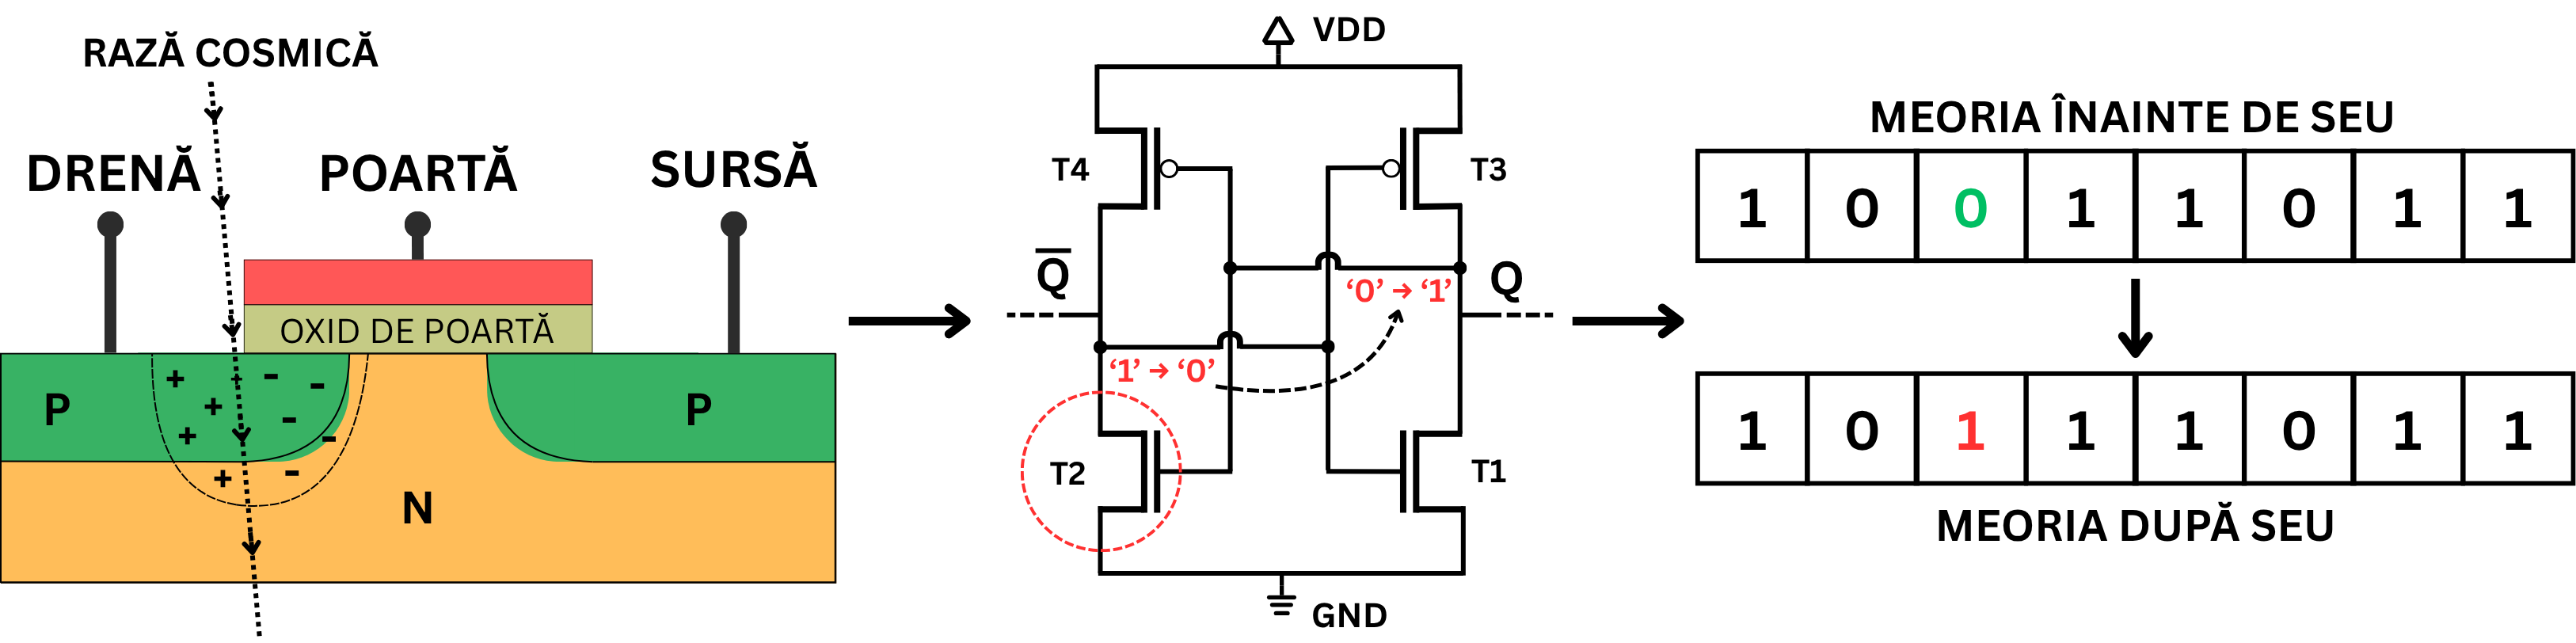
\includegraphics[width=\columnwidth]{./Images/theory_seu_illustration.png}
    \caption{Exemplificarea unui SEU care cauzează un bit-flip într-o celulă SRAM 6T.}%
\label{fig:theory_seu_illustration}
\end{figure}

Consecințele negative apărute din cauza radiației cosmice pot fi clasificate în efecte imediate și efecte de lungă durată. Cu cât un tranzistor de tip Metal–Oxide–Semiconductor (MOS) este expus mai mult timp la o sursă de radiație ionizantă, cu atât acumularea de sarcină parazită crește, schimbându-i caracteristici esențiale precum tensiunea de prag, curentul de scurgere și aspecte privind sincronizarea acestuia.\@ \gls{tid} reprezintă cantitatea de radiație la care poate rezista dispozitivul, până când acesta nu își mai îndeplinește parametrii specificați.\@ \gls{tid} se măsoară în gray (Gy) (unitate care exprimă cantitatea de energie absorbită de un material) și reprezintă o schimbare permanentă și nealterabilă a caracteristicilor electrice ale dispozitivului.

Pe lângă efectele permanente cauzate de radiația cosmică, mai există și perturbări imediate, generate de particule cu energie foarte mare, care pot afecta instantaneu logica internă a unui circuit integrat. Cele mai importante astfel de fenomene sunt descrise în continuare:
\begin{itemize}
    \item \textbf{\gls{seu}}: este un eveniment ce apare când o particulă lovește intrarea unui \gls{ff} sau un tranzistor dintr-o celulă \gls{sram}. Acest eveniment este ilustrat în Figura~\ref{fig:theory_seu_illustration} și funcționează astfel: dacă energia depusă de o particulă individuală este suficientă, se poate crea o schimbare în starea celulei \gls{sram} sau se poate capta o valoare eronată de către \gls{ff}. Un \gls{seu} se propagă ca o greșeală în datele stocate, greșeală care poate duce la erori software. Acesta nu introduce efecte sau modificări permanente la nivelul fizic al componentelor electrice.
    \item \textbf{\gls{sel}}: la dispozitivele construite dintr-un material semiconductor pot apărea anumite structuri care, dacă sunt activate, pot avea efecte neprevăzute și catastrofale. Spre exemplu, în fabricarea circuitelor integrate în tehnologia \gls{cmos} apar și perechi de tranzistori bipolari PNP și NPN care pot forma un tiristor~\cite{parasitic_transistors}. O particulă suficient de energetică poate activa această structură, astfel creându-se o cale de impedanță scăzută între Vdd și Gnd. Dacă alimentarea dispozitivului nu este îndepărtată în scurt timp, acest scurt circuit va distruge circuitul integrat.
    \item \textbf{\gls{set}}: când particula energetică lovește un circuit logic, apare un vârf de tensiune tranzitoriu care se poate propaga prin elementele combinaționale ale circuitului și poate fi captat de un element secvențial, astfel transformându-se într-un \gls{seu}. Dacă acest tranzitoriu nu are suficientă energie pentru a traversa toată logica și pentru a ajunge la un \gls{ff}, evenimentul nu va avea nici-un efect asupra funcționării dispozitivului. Un \gls{set} nu produce efecte fizice permanente, ci poate produce doar erori software.
\end{itemize}

\section{Field-Programmable Gate Array}
La începuturile erei tehnologice, majoritatea circuitelor electronice erau alcătuite din cipuri discrete, fiecare având o funcționalitate simplă și un rol propriu: cipuri pentru operații aritmetice și logice, cipuri de memorie, numărătoare, multiplexoare și decodoare~\cite{74series}. La sfârșitul anilor 1970 însă, procesul \gls{vlsi} și tehnologia \gls{cmos} au permis crearea unor circuite integrate complexe, care îndeplinesc funcții mult mai avansate decât predecesorii lor. Un astfel de Application-Specific Integrated Circuit (ASIC) poate îndeplini toate funcțiile care cu un deceniu în urmă erau îndeplinite de multiple cipuri independente~\cite{intel_4004}\cite{zilog_z80}. În același timp s-au introdus și dispozitive de tip \gls{fpga} ca un răspuns la obstacolele dezvoltării unui ASIC.\@ În principal, \gls{fpga}-urile rezolvă problema costului ridicat al unui circuit integrat și reduc riscul proiectării acestuia prin introducerea capacității de reconfigurare și reprogramare. ASIC-urile moderne au un cost de dezvoltare și fabricație cuprins între 150.000 USD, până la zeci de milioane de USD~\cite{asic_costs_1}\cite{asic_costs_2}. Această sumă se desparte în două categorii diferite: costuri de proiectare și costul per unitate al cipului de siliciu. Procesul de proiectare, sau Non-Recurring Engineering (NRE), este de departe cel mai costisitor aspect al unui ASIC, datorită necesității de a testa și a simula circuitul logic și datorită licențelor și pachetelor de \gls{ip} necesare proiectării acestuia.

\gls{fpga}-urile sunt folosite răspândit pentru prototipare și cercetare, pentru aplicații ce nu necesită un număr suficient de mare de bucăți ca să justifice producerea unui ASIC și pentru controlul proceselor industriale~\cite{basic_fpga}. Cei mai mari producători de dispozitive \gls{fpga} sunt Xilinx și Altera, recent achiziționate de AMD, respectiv Intel. Spre deosebire de ASIC-uri, care odată ce sunt proiectate nu pot fi modificate, un \gls{fpga} este alcătuit din mai multe tipuri de componente reconfigurabile: Configurable Logic Block (CLB)-uri, memorii, blocuri de \gls{io} și trasee de interconectare. CLB-urile sunt componentele de bază ale \gls{fpga}-ului și se găsesc în număr cel mai mare. Ele sunt alcătuite dintr-un \gls{lut} și un adunător, conectate la un \gls{ff}, astfel creându-se o mașină de stări finite în miniatură. Pe lângă CLB-uri, mai pot exista și blocuri Digital
Signal Processing (DSP), care sunt optimizate pentru operații aritmetice dificil de implementat din alte componente logice (multiplicare, divizie, acumulare și combinații ale acestora). La marginea cipului se găsesc blocurile \gls{io}, care conțin diferite tipuri de buffere (unidirecționale și bidirecționale) pentru adaptarea semnalelor la diferitele standarde logice și niveluri de tensiune. Cel mai limitator aspect al unui dispozitiv \gls{fpga} însă, este logica de interconectare. Limitările rețelei de interconectare dintr-un \gls{fpga} reduc drastic frecvența maximă de operare și cresc cantitatea de energie consumată, în comparație cu un ASIC echivalent~\cite{fpga_book}.

Aceste elemente sunt programate prin intermediul unei memorii interne speciale, numită memorie de configurare. Poate fi de mai multe tipuri, precum memorie flash, \gls{eeprom} sau antifuse. În schimb, cea mai des întâlnită este memoria \gls{sram}. Deși este volatilă și nu își menține datele cât timp nu este alimentată, este cel mai folosit tip de memorie datorită vitezei și densității acesteia. Pentru a programa \gls{fpga}-ul este necesară generarea unui fișier bitstream. Crearea acestuia reprezintă un proces îndelungat care este parcurs în mai multe etape:
\begin{itemize}
\item Un inginer hardware scrie o configurare într-un \gls{hdl} precum Verilog, SystemVerilog sau VHSIC Hardware Description Language (VHDL). Aceste limbaje nu sunt ca limbajele de programare software. Ele sunt folosite pentru a descrie comportamentul circuitului integrat la nivel de elemente logice ale unui circuit, precum \gls{ff}-uri, multiplexoare sau porți logice.
\item Într-un fișier \gls{hdl} se definește un modul, având intrări și ieșiri, care îndeplinește un scop precizat. În modul se găsesc fire (wire), prin care se definește logică combinațională, și regiștri (reg), definiți în blocuri always, care stochează valori. 
\item După scriere, fișierul \gls{hdl} este simulat într-un program Electronic Design Automation (EDA) precum Vivado, Quartus sau ModelSim. Se testează funcționalitatea corectă a modulului prin intermediul unui fișier test-bench, sau se generează și se verifică forme de undă pentru semnalele de interes.
\item Dacă modulul hardware a trecut faza de testare, este trecut prin procesele de lintare, sintetizare și implementare. Aceste etape transformă modulul hardware inteligibil uman într-un fișier netlist, care descrie configurarea \gls{fpga}-ului la nivel de porți logice. Nu necesită intervenția utilizatorului și sunt complet automatizate de către programele EDA și Computer-Aided Design (CAD).
\item Fișierul netlist rezultat este apoi transformat într-un fișier cu format binar, numit bitstream, care poate fi încărcat în memoria de configurare a \gls{fpga}-ului prin interfața \gls{jtag}.
\end{itemize}

\section{Printed Circuit Board}
Un \gls{pcb}, sau cablaj imprimat, este o structură alcătuită din două sau mai multe straturi de material izolator și de material conductiv care au rolul de a conecta un ansamblu de componente electronice între ele. Acestea și-au făcut apariția la începutul anilor 1950 și au înlocuit cablajele realizate direct, prin legarea unor fire individuale între bornele componentelor montate pe un șasiu.\@ \gls{pcb}-urile sunt folosite la aproape toate dispozitivele electronice din ziua de azi, iar industria de fabricare a acestora depășește 71 de miliarde USD~\cite{pcb_market_cap}.

Un \gls{pcb} modern poate avea între 2 și 8 straturi pentru aplicațiile comerciale și între 8 și 32 de straturi pentru aplicațiile militare și telecomunicații. Sunt alcătuite din fire metalice aplatizate (numite trace-uri), care fac conexiunea electrică între componente. Cel mai des folosit material este cuprul, ales datorită conductivității sale electrice foarte bune, abilității excelente de a disipa căldura, proprietăților mecanice, dar și datorită prețului acestuia, în comparație cu alte materiale bune conductoare, precum argintul sau aurul. Pentru a conecta două sau mai multe straturi metalice între ele, se folosesc vias-uri. Un via este o gaură făcută în placă, care este ulterior acoperită prin depunere galvanică de cupru~\cite{vias_explination}. Vias-urile pot fi de trei tipuri: through-hole, blind și buried. Vias-urile through-hole trec dintr-un capăt al plăcii până în celălalt, chiar dacă se vrea conectarea a doar două straturi. Blind vias-urile nu trec prin toată placa, ci sunt vizibile doar pe o parte a \gls{pcb}-ului, iar buried vias-urile se află complet în interiorul plăcii și, în consecință, conectează doar straturi interne. 

Pentru a izola electric straturile metalice și pentru a oferi o structură rigidă \gls{pcb}-ului, se introduc straturi făcute dintr-un material dielectric, confecționate din hârtie sau țesătură, impregnate cu diferite tipuri de rășină. Aceste materiale sunt alese și combinate pentru a îmbunătăți proprietățile electrice și mecanice adaptate aplicației. Cel mai întâlnit tip de dielectric este FR-4 (țesătură din fibră de sticlă impregnată cu o rășină epoxidică ignifugă), ales pentru costul redus, proprietăți electrice excelente (rezistență dielectrică ridicată și pierderi dielectrice reduse) și rezistență structurală și la foc. FR-4 este suficient în majoritatea situațiilor comerciale și industriale, însă pentru anumite aplicații ce necesită lucrul cu frecvențe foarte mari sau lucrul în spațiu, se folosesc materiale mai scumpe și mai performante precum CEM-1, CEM-3, PTFE sau materiale flexibile precum poliamidă~\cite{pcb_materials}. La finalul procesului de fabricare al unui \gls{pcb} se acoperă suprafața acestuia cu un strat de epoxy fotosensibil izolator numit solder mask. Acesta protejează straturile externe de cupru de mediul înconjurător și de evenimente accidentale de scurt-circuit și oferă culoarea caracteristică unui \gls{pcb} (verde, roșu, albastru sau alte culori).

\begin{figure}[h!]
    \centering
    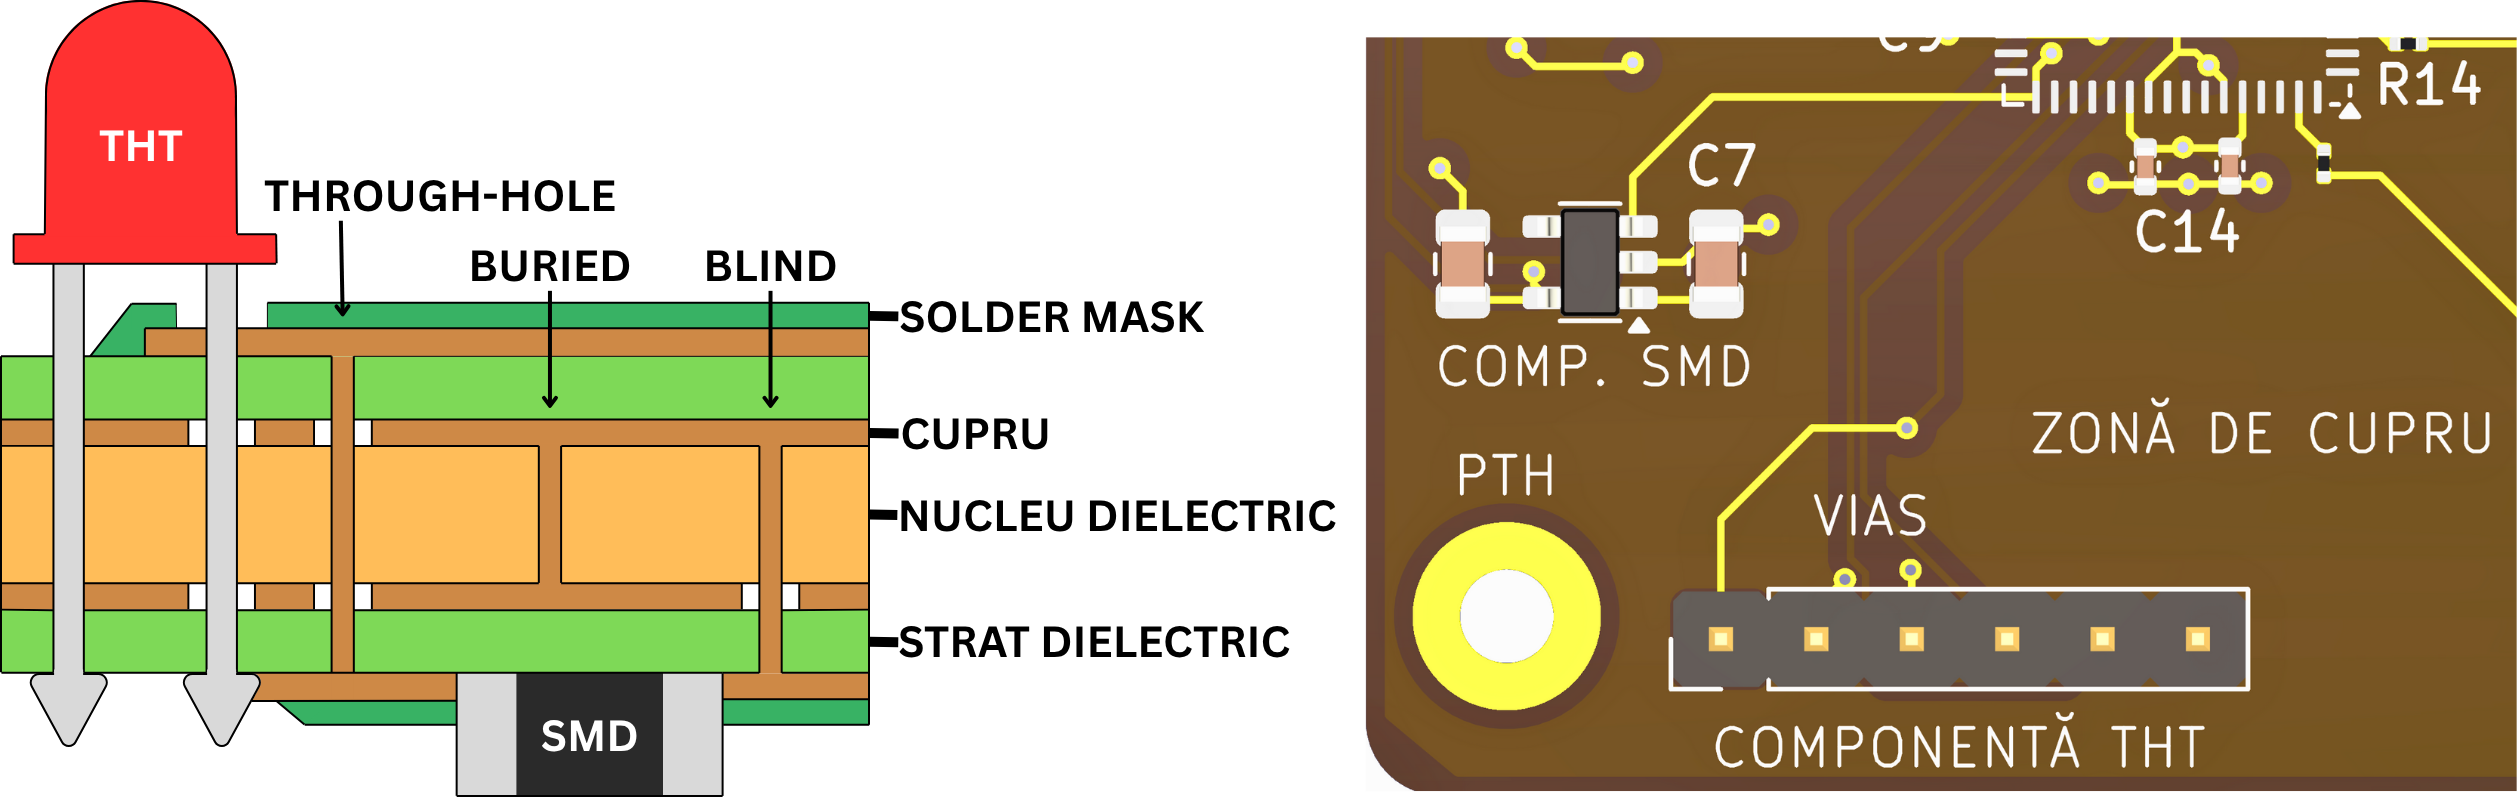
\includegraphics[width=\columnwidth]{./Images/theory_pcb_cross_section.png}
    \caption{Structura unui PCB cu patru straturi, cu componente THT și SMD.}%
\label{fig:theory_pcb_cross_section}
\end{figure}

Structura transversală și cea longitudinală a unui \gls{pcb} sunt ilustrate în Figura~\ref{fig:theory_pcb_cross_section}. Sunt exemplificate tipurile de vias-uri și de componente, precum și structura internă a unui cablaj imprimat. Mai departe vor fi definiți și explicați diverși termeni de interes pentru proiectarea și fabricarea unui \gls{pcb}, cum ar fi tipurile de găuri metalizate și nemetalizate, scrierea de text, ilustrații, trasee și componente:
\begin{itemize}
\item Firele aplatizate ce aparțin straturilor metalice se numesc \textit{trasee} (traces) și, la rândul lor, pot fi de mai multe tipuri. Toate traseele de pe straturile exterioare se numesc microstrip și sunt folosite pentru a reduce costul de fabricație și pentru a ușura accesul și procesul de depanare. Traseele de pe straturile interioare se numesc stripline. Acestea sunt folosite pentru a avea un control mult mai mare asupra impedanței și integrității semnalului. În funcție de tipul de semnal transmis printr trasee, acestea pot fi single-ended sau diferențiale. În cazul perechilor diferențiale, trebuie să se acorde o atenție deosebită dimensiunilor fiecărui traseu și distanței între ele, pentru a menține impedanța caracteristică interfeței de comunicație.
\item Exista două tipuri de găuri mecanice prezente pe un \gls{pcb}. Toate găurile care au un strat de metalizare pe lungimea acestora (ca și în cazul vias-urilor) se numesc \textit{\gls{pth}}, pe când toate cele ce nu sunt metalizate se numesc \textit{\gls{npth}}. Găurile \gls{pth} sunt folosite atunci când se dorește conectarea a mai multor straturi metalice între ele sau la lipirea pinilor componentelor electrice. Cele \gls{npth} sunt pur mecanice și se folosesc de obicei pentru montare.
\item Un \gls{pcb} poate fi proiectat pentru a conecta două tipuri diferite de componente, caracterizate de modalitatea de atașare a acestora. Componentele \textit{\gls{tht}} se folosesc de fire conectoare, care sunt inserate prin placă și lipite pe partea opusă. Componentele de tip \textit{\gls{smd}} se debarasează de aceste fire și sunt lipite direct pe partea plăcii la care sunt atașate.
\item Când o componentă este plasată pe placă, ea este reprezentată grafic de un \textit{footprint}. Majoritatea componentelor electrice au o forma și un pachet standardizat, cele mai des întâlnite tipuri fiind: i) pini de o parte și de alta a componentei dreptunghiulare (Small Outline Integrated Circuit, SOIC), ii) pini pe toate cele patru laturi unei componente pătrate (Quad Flat Package, QFP), iii) pini integrați direct în carcasa circuitului integrat (Quad Flat No-lead, QFN) și iv) mici bile de metal dispuse într-o matrice pe partea inferioară a capsulei (Ball Grid Array, BGA). Ultimul tip enumerat este folosit cel mai des pentru procesoare, \gls{fpga}-uri și circuite integrate complexe, ce necesită un număr de pini foarte mare. Cu cât crește nivelul de integrare a capsulei, cu atât crește și complexitatea procesului de lipire a componentei pe \gls{pcb}, precum și dificultatea de rutării traseelor către pini.
\item Ordinea de aranjare a straturilor metalice și dielectrice, împreună cu definirea dimensiunii acestora, tipului de material și constantele dielectrice, sunt organizate într-un tabel numit \textit{stackup}.
\item Orice text, grafică sau linii explicative care sunt imprimate pe \gls{pcb} în culoarea alb (cea mai des utilizată, datorită contrastului oferit fată de culoarea solder mask-ului. Pentru solder mask de culoarea albă, se folosește text negru)  sunt definite în stadiul de proiectare pe un strat special numit \textit{silkscreen}.
\end{itemize}

% ---------------------------------------------------------------

\chapter{Proiectarea și implementarea sistemelor pe FPGA}
\section{Alegerea FPGA-ului ideal}
Fiind componenta centrală a sistemului, alegerea dispozitivului \gls{fpga} ideal a fost realizată cu deosebită atenție, cu obiectivele de a minimiza consumul de energie electrică și de a oferi o eficacitate cât mai mare senzorului, fie prin dimensiunea elementului detector, fie prin creșterea secțiunii transversale. Rezultatele preliminare ale acestui proces de selecție sunt prezentate în~\cite{jes} și vor fi detaliate în secțiunile următoare. Au fost testate și comparate cele mai performante două dispozitive din fiecare dintre familiile Artix-7 și Artix UltraScale+, precum și cele mai puțin performante două dispozitive din seria Kintex UltraScale+ (US+)~\cite{7series_product_selection, ultrascale_product_selection}. Sunt prezente doar \gls{fpga}-uri produse de Xilinx, și nu Intel (fost Altera), deoarece experiența anterioară a echipei s-a concentrat exclusiv pe această platformă. De asemenea, laboratorul în care s-a desfășurat proiectul dispunea deja de două plăci de dezvoltare cu \gls{fpga}-uri Xilinx, ceea ce a favorizat utilizarea acestui ecosistem și a redus necesitatea de achiziții suplimentare și de formare pe alte arhitecturi. Alți producători mai mici, precum Lattice sau Microchip nu au fost luați în considerare din cauza suportului software limitat și pentru că majoritatea produselor acestora sunt orientate fie aplicațiilor comerciale simple, fie unora mult prea specializate.

\subsection{Analiză a produselor disponibile}
Paralela între \gls{fpga}-urile analizate este prezentată în Tabelul~\ref{tab:sw_fpga_comparison}. Sunt incluse informații privind denumirea și familia fiecărui dispozitiv, numărul de resurse logice disponibile, capacitatea memoriei de tip \gls{bram}, precum și cel mai mic preț găsit pentru o singură unitate. Dintre toți parametrii considerați, cei mai importanți au fost numărul de memorii \gls{bram}, fiind esențiale pentru implementarea detectorului de radiație, precum și prețul unității. Un număr mai mare de \gls{bram}-uri permite o implementare mai eficientă a senzorului, în timp ce un preț redus ajută la fabricarea și popularea unui număr mai mare de plăci, facilitând testarea extinsă și experimentarea în diverse scenarii. Deși dispozitivele din familia Kintex US+ au cele mai multe resurse logice și includ,  pe lângă memoria \gls{bram}, un tip adițional numit \gls{uram}~\cite{fpga_memory_types}, cu dimensiunea fiecărui bloc de 288 Kb, acestea sunt prea costisitoare pentru aplicația vizată. În plus, au un număr de \gls{bram}-uri similar cu celelalte opțiuni mult mai accesibile. De exemplu, modelul KU5P este de 8.3 ori mai scump decât XC7A200T, oferind doar cu 24\% mai multe memorii \gls{bram}. Din aceleași motive, au fost excluse și dispozitivele din familia Artix US+, acestea având mai puține memorii decât predecesorii lor din seria Artix-7, fără a aduce avantaje semnificative care să justifice creșterea prețului. În plus, capsulele dispozitivelor US+ sunt mai mari (23 mm sau 27 mm) decât Artix-7 (19 mm), ceea ce îngreunează integrarea acestuia într-un \gls{pcb} compact impus de aplicația spațială.

\begin{table}[ht!]
  \centering
  \renewcommand{\arraystretch}{1.6}
  \caption{Analiză comparativă a unor FPGA-uri similare.}%
  \label{tab:sw_fpga_comparison}
  \begin{tabular}{l c c c c c c c r}
    \toprule
    \textbf{Familie} & \textbf{Nume} & \textbf{FF} & \textbf{LUT} & \textbf{DSP} & \textbf{URAM} & \textbf{BRAM} & \textbf{BRAM [Kb]} & \textbf{Preț} \\
    \midrule
    Artix-7 & XC7A100T & 126.800 & 63.400 & 240 & --- & 135 & 4.860 & \$258 \\
    Artix-7 & XC7A200T & 269.200 & 134.600 & 740 & --- & 365 & 13.140 & \$370 \\
    \midrule
    Artix US+ & AU20P & 218.000 & 109.000 & 900 & --- & 200 & 7.200 & \$587 \\
    Artix US+ & AU25P & 282.000 & 141.000 & 1200 & --- & 300 & 10.800 & \$700 \\
    \midrule
    Kintex US+ & KU3P & 325.440 & 162.720 & 1368 & 48 & 360 & 12.960 & \$2252 \\
    Kintex US+ & KU5P & 433.920 & 216.960 & 1824 & 64 & 480 & 17.280 & \$3056 \\
    \bottomrule
  \end{tabular}
\end{table}

\subsection{Sensibilitatea la radiație}
În final a fost ales dispozitivul XC7A200T din familia Artix-7, datorită raportului \gls{bram}-preț cel mai bun, dar și pentru numărul de resurse logice adecvate cerințelor aplicației. Deși familia Artix-7 este considerată relativ învechită (primele produse fiind lansate din 2012) și este realizată printr-un proces de fabricație pe 28 nm, trebuie avută în vedere și sensibilitatea acestora la radiația cosmică. Valorile prezentate în Tabelul~\ref{tab:sw_fpga_cross_section} sunt preluate din~\cite{amd_reliability_report}, unde este documentată fiabilitatea dispozitivelor de la Xilinx, în special sensibilitatea și secțiunea transversală a memoriilor \gls{bram} și \gls{cram} pentru diferite familii de \gls{fpga}-uri, în urma testelor realizate la \gls{lansce}. În cadrul experimentelor a fost inclusă și memoria \gls{cram} pentru că este, la rândul său, sensibilă la radiația cosmică. Mai mult, aceasta joacă un rol esențial în buna funcționare a dispozitivului, fiind responsabilă pentru stocarea configurației interne a \gls{fpga}-ului. Comparativ cu memoria \gls{bram}, \gls{cram}-ul este mult mai extins, ajungând la o capacitate de 74 Mb în cazul dispozitivului XC7A200T, față de doar 13 Mb de memorie \gls{bram}.

\begin{table}[h!]
  \centering
  \renewcommand{\arraystretch}{1.6}
  \caption{Secțiunea transversală și rata de erori pentru diverse familii de FPGA-uri.}%
  \label{tab:sw_fpga_cross_section}
  \begin{tabular}{c c C{3.6cm} C{3.6cm} C{1.6cm} C{1.6cm}}
    \toprule
    \textbf{Tehnologie} & \textbf{Familie} & \textbf{Sec.\ transversală BRAM [cm\textsuperscript{2} / bit]} & \textbf{Sec.\ transversală CRAM [cm\textsuperscript{2} / bit]} & \textbf{FIT/Mb BRAM} & \textbf{FIT/Mb CRAM}\\
    \midrule
    28 nm & Artix-7 & \(6.32 \times 10^-15\) & \(6.99 \times 10^-15\) & 72 & 74 \\
    28 nm & Kintex-7 & \(5.57 \times 10^-15\) & \(5.69 \times 10^-15\) & 42 & 40 \\
    20 nm & UltraScale & \(4.43 \times 10^-15\) & \(2.55 \times 10^-15\) & 58 & 32 \\
    16 nm & UltraScale+ & \(9.82 \times 10^-16\) & \(2.67 \times 10^-16\) & 15 & 5 \\
    \bottomrule
  \end{tabular}
\end{table}

Secțiunea transversală este definită ca probabilitatea ca o particulă energetică să producă un \gls{see}, cum ar fi un \gls{seu} sau un latch-up, și se exprimă în \(cm^2/bit\) sau \(cm^2/dispozitiv\). De asemenea, un Failure in Time (FIT) corespunde unei defecțiuni la un miliard de ore de funcționare a dispozitivului. Cu cât secțiunea transversală este mai mare, cu atât \gls{fpga}-ul este mai sensibil la radiație, ceea ce implică creșterea numărului de erori și, implicit, numărul de FIT-uri. În contextul aplicației curente, acest aspect este însă favorabil. Se poate observa că familia Artix-7 este, în medie, de zece ori mai sensibilă la radiație decât familia US+, ceea ce permite o detecție mai eficientă a particulelor energetice.

\subsection{Analiză a consumului de energie}
Un alt aspect esențial în alegerea dispozitivului este consumul de energie. Pentru a evalua acest parametru, s-a folosit o versiune preliminară a programului dedicat detecției \gls{seu}-urilor, prezentat în~\cite{isetc} și descris în detaliu în Capitolul”\ref{seu_program_implementation}. Programul populează 100 de blocuri \gls{bram} cu un șablon cunoscut de valori, apoi le scanează secvențial pentru a detecta eventualele bit-flip-uri cauzate de radiație. Testarea s-a realizat folosind trei variante ale aceluiași proiect, rulat la frecvențele de 10 MHz, 50 MHz și 100 MHz, pentru a observa dependența între consumul dinamic de energie și frecvența de operare. Simularea consumului de energie a fost realizată folosind unealta integrată de estimare a puterii din cadrul AMD Vivado 2024.1, pentru cele mai performante \gls{fpga}-uri din fiecare dintre cele trei familii analizate: Artix-7, Artix US+ și Kintex US+. Rezultatele sunt prezentate în Figura~\ref{fig:fpga_power_estimations}, precum și în~\cite{jes}. Chiar dacă au fost folosiți aceiași parametri de intrare și aceleași constrângeri pentru toate simulările, se poate observa un consum static de 4.4 ori mai mic pentru dispozitivul XC7A200T, față de celelalte două \gls{fpga}-uri. Deși consumul său dinamic este cu aproximativ 15\% mai ridicat, \gls{fpga}-ul Artix-7 este cel mai eficient din punct de vedere energetic, ceea ce reprezintă un argument în plus pentru alegerea acestui dispozitiv.

\begin{figure}[h]
    \centering
    \begin{tikzpicture}
        \begin{groupplot}[
            ybar,
            /pgf/bar width=16pt,
            enlarge x limits=0.22,
            enlarge y limits=0.3,
            ylabel={Putere [mW]},
            symbolic x coords={100 MHz, 50 MHz, 10 MHz},
            xtick=data,
            width=8.5cm,
            height=7cm,
            grid=major,nodes near coords,
            tick label style={font=\footnotesize},
            every node near coord/.append style={font=\footnotesize},
            legend style={at={(1.1,-0.2)}, anchor=north, legend columns=3, column sep=7pt},
            group style={group size=2 by 1,horizontal sep=1cm,ylabels at=edge left,vertical sep=0pt}
        ]
        
        % First plot
        \nextgroupplot[title={Consum static}]
        \addplot+[blue, fill=blue!20] coordinates {(100 MHz,  103)(50 MHz,  103)(10 MHz, 102)};
        \addlegendentry{XC7A200T}
        \addplot+[red, fill=red!20] coordinates {(100 MHz,  457)(50 MHz,  455)(10 MHz, 453)};
        \addlegendentry{AU25P}
        \addplot+[brown, fill=brown!20] coordinates {(100 MHz,  457)(50 MHz,  455)(10 MHz, 453)};
        \addlegendentry{KU5P}
        
        % Second plot
        \nextgroupplot[title={Consum dinamic}]
        \addplot+[blue, fill=blue!20] coordinates {(100 MHz,  626)(50 MHz,  366)(10 MHz, 159)};
        \addplot+[red, fill=red!20] coordinates {(100 MHz,  473)(50 MHz,  291)(10 MHz, 140)};
        \addplot+[brown, fill=brown!20] coordinates {(100 MHz,  475)(50 MHz,  290)(10 MHz, 140)};
        
        \end{groupplot}
    \end{tikzpicture}
    \caption{Consumul de energie pentru FPGA-urile din cele trei familii.}%
\label{fig:fpga_power_estimations}
\end{figure}

\section{Structura generală a proiectului Verilog}
\label{sw_general_structure}
Întregul proiect destinat implementării detectorului de \gls{seu}-uri, precum și al sistemelor de comunicație externă și auxiliare, a fost dezvoltat în limbajul Verilog și este ilustrat în Figura~\ref{fig:sw_general_diagram}. Dezvoltarea acestor module a fost realizată folosind AMD Vivado 2024.1, iar pentru proiectele de test bazate pe procesorul MicroBlaze au fost utilizate programele AMD Vivado 2024.2 și AMD Vitis 2024.2. Verilog, la fel ca celelalte limbaje de descriere hardware, se bazează pe module individuale ce îndeplinesc o funcție specifică, conectate între ele prin semnale de diverse lățimi. Diagrama prezentată în Figură evidențiază modulul Top, care, după cum sugerează și denumirea, reprezintă modulul de nivel superior, care încapsulează restul blocurilor funcționale. În centrul diagramei se află modulul \gls{du}, responsabil cu instanțierea tuturor elementelor de detecție, stocarea erorilor identificate într-un buffer intern de tip \gls{fifo}, precum și inserarea manuală de erori prin cele patru fire INJ.\@ Această interfață are un rol esențial atât în simularea corectă a programului, cât și în lipsa unei surse de radiație ionizantă în laborator, care ar permite testarea \gls{fpga}-ului în condiții reale de iradiere. Semnalele INJ sunt generate de blocul \gls{vio}, un \gls{ip} oferit de Xilinx care permite interfațarea directă cu un calculator prin intermediul interfeței \gls{jtag}. Acest bloc suportă atât semnale de intrare, cât și de ieșire, facilitând injectarea de erori și observarea comportamentului sistemului în timpul testelor.

\begin{figure}[h!]
    \centering
    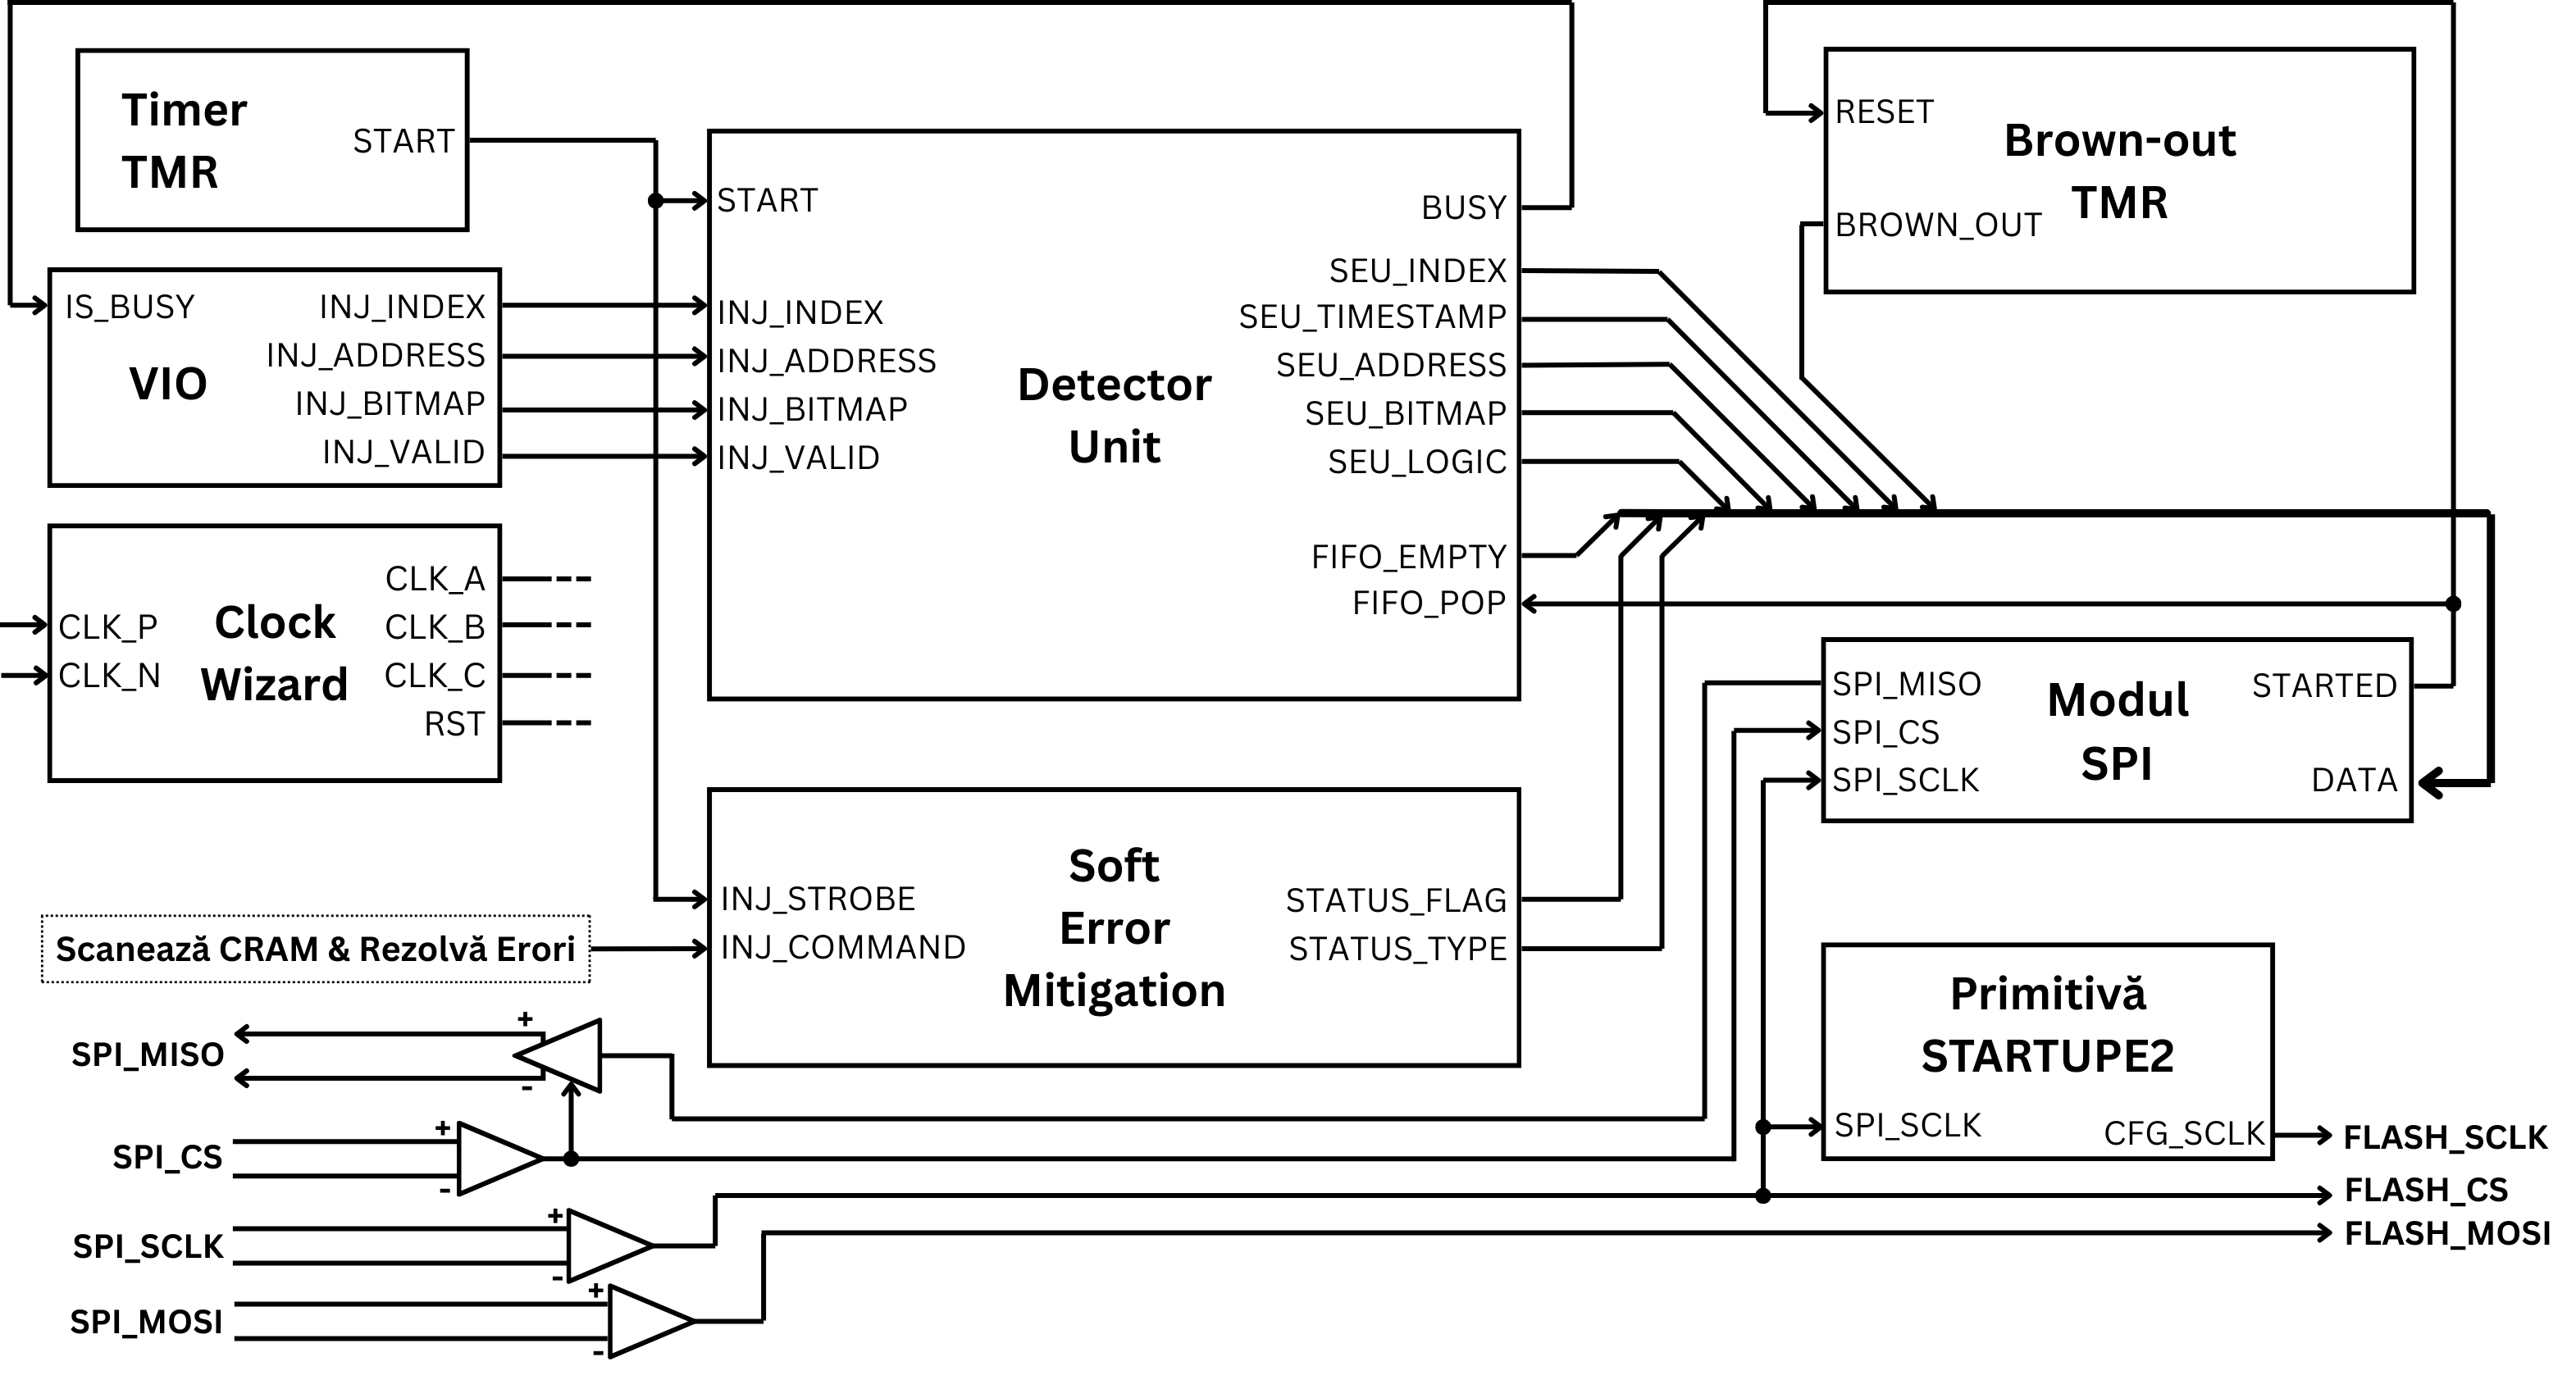
\includegraphics[width=\columnwidth]{./Images/sw_general_diagram.png}
    \caption{Schema bloc a modulului Top scris în Verilog.}%
\label{fig:sw_general_diagram}
\end{figure}

Sub blocul \gls{du} se află \gls{ip}-ul \gls{sem}, folosit pentru scanarea automată a memoriei \gls{cram}, identificarea și clasificarea severității erorilor detectate, precum și corectarea acestora acolo unde este posibil. Acest modul este esențial pentru menținerea \gls{fpga}-ului într-o stare funcțională cât mai mult timp posibil și pentru a identifica cât mai multe erori, astfel crescând eficiența întregului detector (\gls{fpga}-ul ales având de 5.7 ori mai multă memorie de configurare decât memoria \gls{bram}). Implementarea și testarea sa sunt detaliate în Capitolul~\ref{sem}

Începerea unui ciclu de scanare a memoriilor \gls{bram} și \gls{cram} se face cu ajutorul unui timer implementat cu redundanță \gls{tmr}, activat la intervale predefinite. Frecvența acestuia este presetată de utilizator și trebuie să fie suficient de mare pentru a asigura detecția rapidă a erorilor, precum și stocarea acestora într-un buffer pentru transmiterea către \gls{obc}. Sub timer se regăsește generatorul de ceas, un circuit proprietar Xilinx care preia un semnal de ceas extern și îl convertește într-un semnal stabil, cu frecvența programabilă. Se pot observa două semnale de intrare, provenite de la oscilatorul \gls{lvds} ce se folosește de o interfață diferențială, precum și trei semnale de ieșire. Acestea sunt identice din punct de vedere al frecvenței și fazei, și sunt folosite în paralel la implementarea sistemului \gls{tmr}. Folosirea a trei semnale de ceas independente scade posibilitatea apariției unor erori datorate interferențelor electrice apărute din cauza radiației.

În colțul din dreapta sus a imaginii este prezent un registru \gls{tmr} responsabil de detectarea evenimentelor de tip brown-out și transmiterea acestora către \gls{obc}. Acesta este inițializat cu valoarea \enquote{1} și este resetat la valoarea \enquote{0} după prima tranzacție 
\gls{spi}. În contextul unui nanosatelit, un brown-out apare atunci când satelitul se reorientează și alocă toată energia electrică disponibilă sistemelor de control al atitudinii, reducând semnificativ alimentarea modulelor experimentale. Astfel, se pot pierde toate erorile de tip \gls{seu} acumulate în \gls{fifo} care nu au fost transmise către \gls{obc} și stocate într-o memorie non-volatilă.

Comunicația cu \gls{obc}-ul este realizată prin modulul \gls{spi} situat în partea dreaptă a diagramei. Acesta, la inițializarea unei tranzacții (prin activarea semnalului \gls{cs}), încarcă toate datele de interes (prin firele SEU, STATUS și altele) într-un shift register și le transmite serial prin linia \gls{miso}. Deoarece comunicația este unidirecțională (de la \gls{fpga} către \gls{obc}), linia \gls{mosi} poate fi reutilizată pentru programarea cipului de memorie flash ce stochează fișierele de configurare ale \gls{fpga}-ului. Astfel se poate implementa abilitatea de a reprograma \gls{fpga}-ul în spațiu, fără necesitatea unui calculator conectat prin interfața \gls{jtag}. Acest lucru se poate face simultan și fără conflicte electrice, deoarece fiecare dintre cele două sisteme comunică doar într-o singură direcție. Pentru a putea interconecta pinii \gls{io} de la cipul flash cu cei ai interfeței \gls{lvds} \gls{spi}, este necesară conversia între protocoalele \gls{lvds} și Low-Voltage CMOS 3.3V (LVCMOS33). Aceasta este realizată automat în mare parte de \gls{fpga}, cu ajutorul bufferelor de tip OBUFDS și IBUFDS oferite de Xilinx~\cite{7series_select_io}, care transformă un semnal diferențial de ieșire sau de intrare, în semnale single-ended. Apare o problemă, însă, la conectarea pinului de ceas destinat cipului flash. Acesta este un pin de configurare special al \gls{fpga}-ului și nu poate fi controlat direct prin folosirea unei constrângeri obișnuite. Pentru a putea transmite semnale către acest pin după etapa de configurare a \gls{fpga}-ului, este necesară instanțierea primitivei STARTUPE2. Această primitivă facilitează accesul utilizatorului la semnale interne critice ale \gls{fpga}-ului, de exemplu semnalele globale de reset și ceas, precum și pinii externi de status~\cite{ug953}.

\section{Arhitectura și implementarea elementului detector}%
\label{seu_program_implementation}

Principiul de funcționare al modulului \acrfull{du} constă în scanarea simultană a unui număr de memorii \gls{bram} și \gls{lutram}, și compararea valorilor stocate cu un șablon de referință, cu scopul de a detecta bit-flip-uri cauzate de evenimentele de tip \gls{seu}. Memoriile \gls{bram} disponibile în familia Artix-7 sunt de tip dual port și au o capacitate de 36 Kb, ce poate fi configurată în diferite formate. În~\cite{isetc} au fost prezentate motivele alegerii dimensiunii de 2048 de adrese cu o lățime de 18 biți per cuvânt. 

Pentru a fundamenta această alegere, au fost testate toate configurațiile posibile de \gls{bram} într-un proiect simplificat, cu structura asemănătoare modulului \gls{du}. În cadrul testelor, s-a măsurat consumul de resurse pentru fiecare variantă, iar rezultatele au fost preluate și ilustrate în Tabelul~\ref{tab:sw_bram_aspect_ratios}. Din aceste date se poate observa faptul că numărul de \gls{lut}-uri și \gls{ff}-uri crește odată cu lățimea unui cuvânt, iar viteza de scanare a fiecărui bloc \gls{bram} scade de două ori la fiecare înjumătățire a spațiului de adrese. Configurația 2048 $\times$ 18 reprezintă un compromis optim între rata de scanare și utilizarea eficientă a resurselor logice, păstrând un spațiu de adrese suficient de mare, fără a crește drastic numărul de \gls{lut}-uri. Valorile scrise în memorie sunt alcătuite dintr-o succesiune de biți '1' și '0' pentru adresele pare, iar inversul acestora pentru adresele impare. Astfel se asigură o distribuție echilibrată de biți \enquote{1} și \enquote{0}, ceea ce contribuie la omogenizarea memoriei și permite detectarea uniformă a bit-flip-urilor produse de \gls{seu}-uri.

\begin{table}[h!]
  \centering
  \renewcommand{\arraystretch}{1.3}
  \caption{Utilizarea resurselor de către DE pentru toate dimensiunile BRAM.}%
  \label{tab:sw_bram_aspect_ratios}
  \begin{tabular}{L{2cm} C{1.65cm} C{1.65cm} C{1.65cm} C{1.65cm} C{1.65cm} C{1.65cm} C{1.65cm}}
    \toprule
    \textbf{Raport} & \textbf{512 $\times$ 72} & \textbf{1K $\times$ 36} & \textbf{2K $\times$ 18} & \textbf{4K $\times$ 9} & \textbf{8K $\times$ 4}  & \textbf{6K $\times$ 2} & \textbf{2K $\times$ 1}\\
    \midrule
        \textbf{LUT-uri} & 246 & 173 & 134 & 122 & 116 & 124 & 128 \\
        \textbf{FF-uri} & 342 & 246 & 204 & 189 & 186 & 192 & 201 \\
        \textbf{Dim. [Kb]} & 36 & 36 & 36 & 36 & 36 & 32 & 32 \\
    \bottomrule
  \end{tabular}
\end{table}

În cazul programului prezentat în~\cite{isetc}, au fost utilizate doar 100 de blocuri de memorie \gls{bram} pentru evaluarea consumului de energie și de resurse, diminuând astfel timpul necesar pentru sintetizarea și implementarea fiecărei versiuni a programului. În cadrul proiectului de față, însă, se dorește utilizarea a numărului maxim de memorii pentru maximizarea performanței senzorului de radiație. Astfel, au fost instanțiate 356 de memorii \gls{bram} dintr-un total de 365 disponibile pe \gls{fpga}. Blocurile rămase au fost alocate altor componente esențiale, precum modulul \gls{sem}, sisteme de test (Debug Hub, Integrated Logic Analyzer (ILA)\cite{ug908}), sau un procesor MicroBlaze. În plus, au fost implementate și blocuri de memorie identice cu cele \gls{bram}, folosind primitive \gls{lutram}. Acestea au dimensiunea de 128 de adrese cu o lățime a cuvântului de 1 bit, însă au fost aranjate pentru a permite o dimensiune parametrizabilă. Numărul maxim de astfel de instanțe este 40, iar detaliile privind implementarea lor sunt prezentate în Capitolul~\ref{lutram}.

\subsection{Detector Unit (DU)}
Modulul \acrfull{du} integrează toată logica necesară pentru detectarea erorilor cauzate de \gls{seu}-uri. Acesta include instanțierea memoriilor de detecție, scanarea ciclică a acestora, memorarea numărului de cicluri efectuate, identificarea erorilor de tip bit-flip, stocarea acestora într-un buffer \gls{fifo} și transmiterea lor către blocul de comunicație \gls{spi}. Schema bloc a modulului este ilustrată în Figura~\ref{fig:sw_du_general_diagram} și va fi detaliată în continuare. 

\begin{figure}[h!]
    \centering
    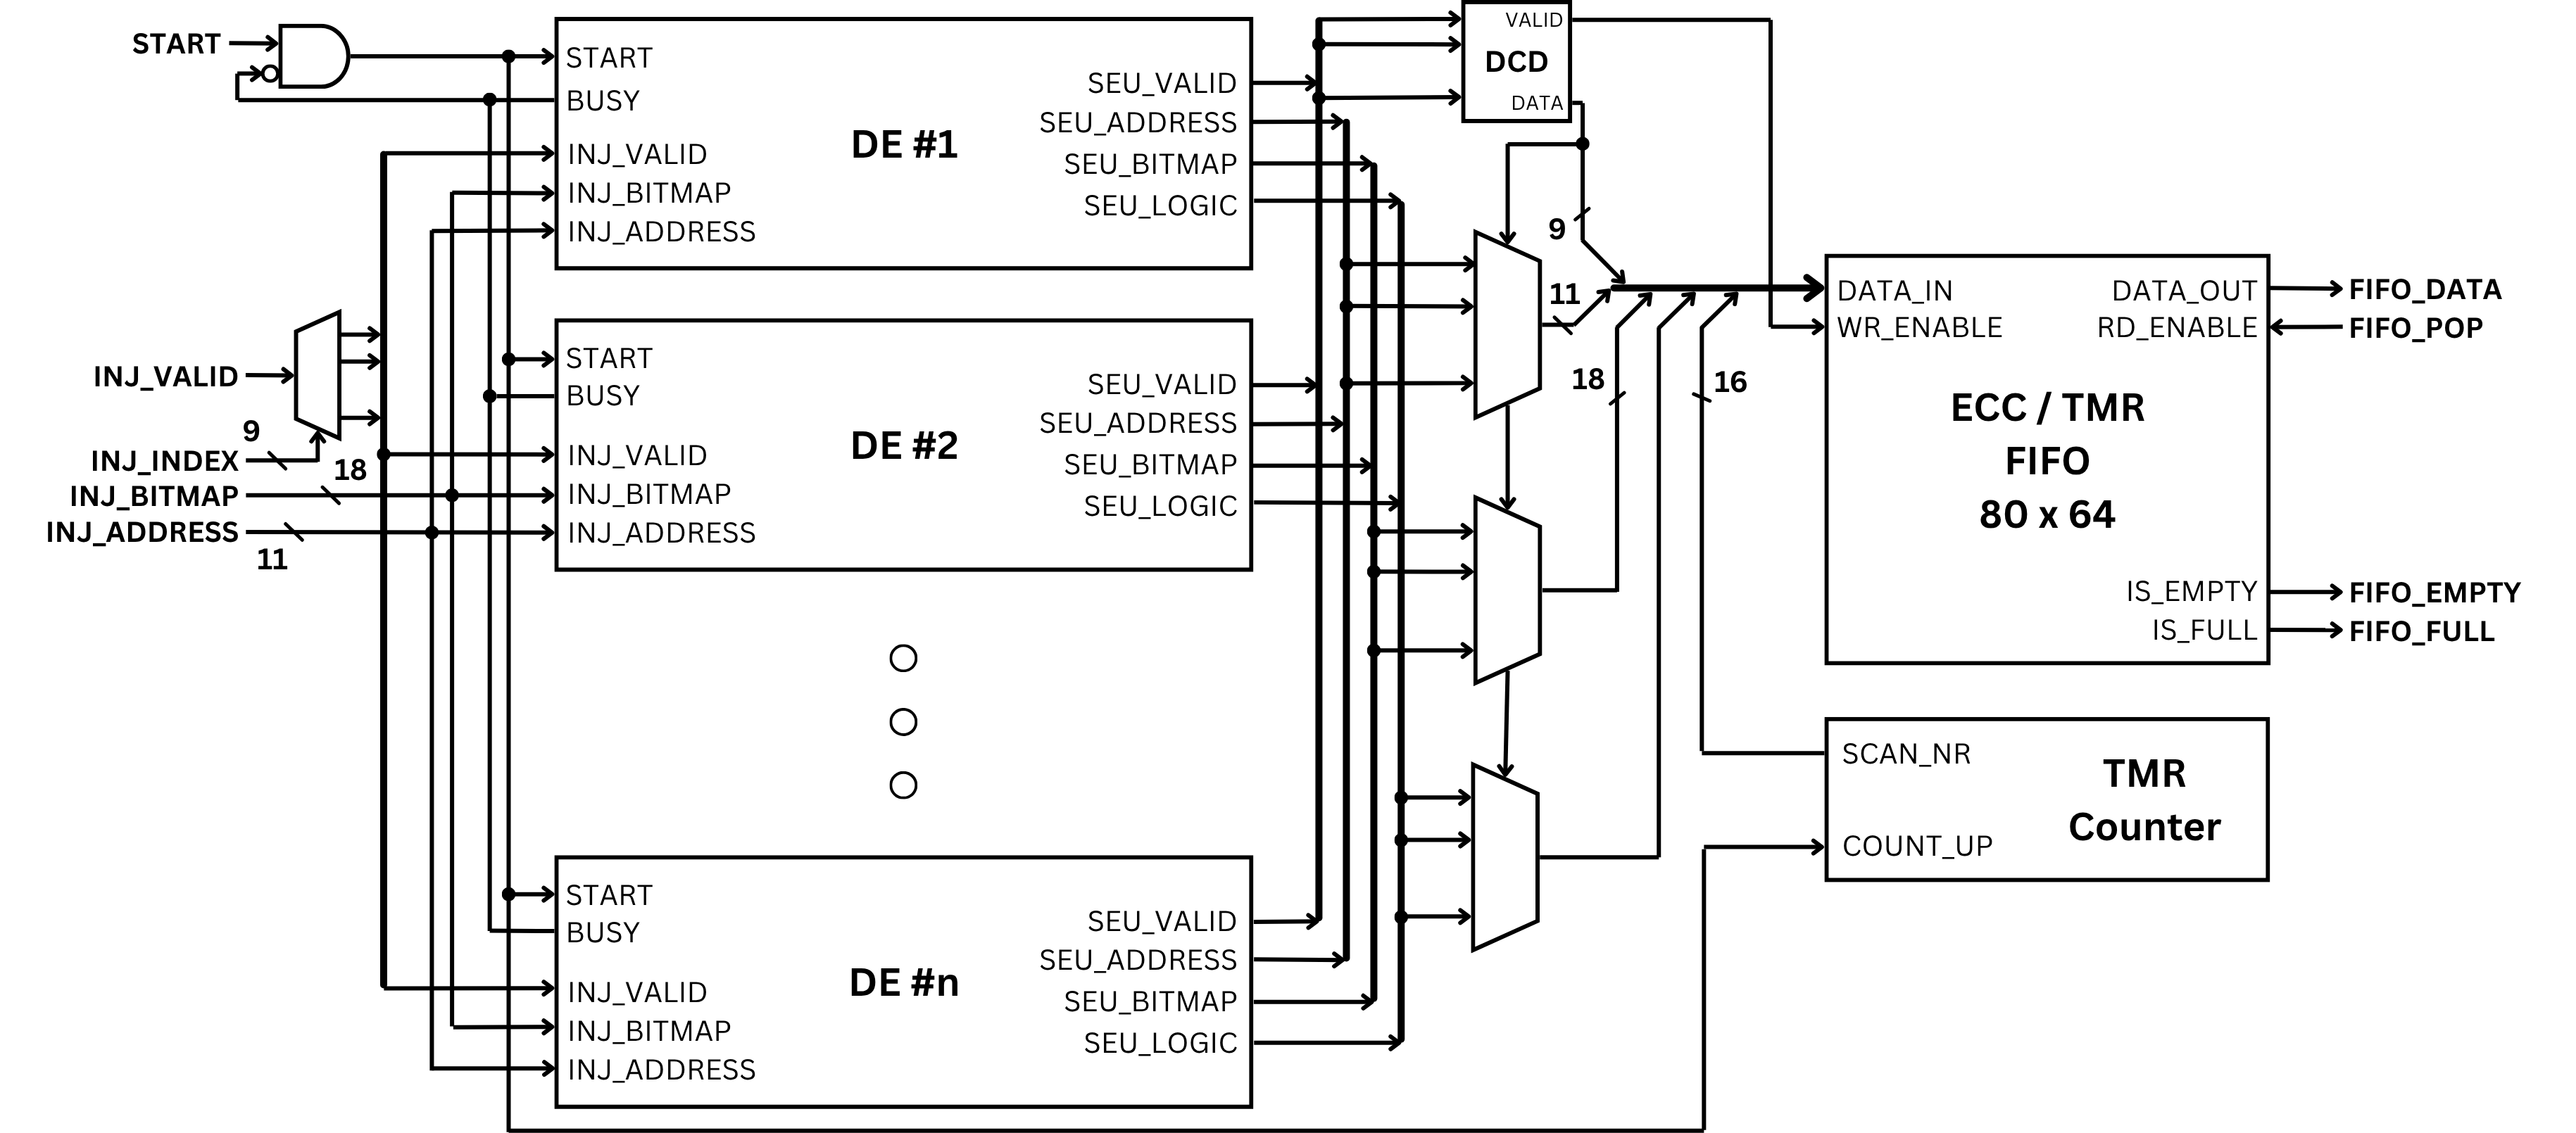
\includegraphics[width=\columnwidth]{./Images/sw_du_general_diagram.png}
    \caption{Schema bloc a modulului Detector Unit (DU).}%
\label{fig:sw_du_general_diagram}
\end{figure}

Este instanțiat un număr parametrizabil de module \gls{de}, fiecare având două semnale de control, trei intrări pentru injectarea de erori (INJ) și patru ieșiri pentru raportarea acestora (SEU). Semnalele de control sunt intrarea START și ieșirea BUSY, legate între ele pentru a preveni inițierea unei noi scanări înainte de finalizarea celei curente, protejând astfel logica de detecție. Semnalul FIFO\_POP provine din modulul \gls{spi} și este activat la inițierea fiecărei tranzacții între \gls{fpga} și \gls{obc}. Acesta are rolul de a extrage datele din \gls{fifo} și de a reseta contorul de cicluri. 

Cele trei intrări INJ reprezintă adresa de inserare a erorii, valoarea acesteia și semnalul de enable. Acestea sunt comune tuturor instanțelor \gls{de}, cu excepția semnalului de enable, care este activ doar dacă semnalul INJ\_INDEX corespunde indexului detectorului respectiv. Ieșirile fiecărui \gls{de} sunt formate din adresa erorii, valoarea citită, un semnal de activare și un semnal suplimentar SEU\_LOGIC, utilizat pentru identificarea erorilor combinaționale. Acest ultim semnal indică faptul că la unul dintre registrele protejate prin \gls{tmr} a apărut o neconcordanță în valorile stocate. Circuitul specific și modul de funcționare sunt detaliate în Capitolul~\ref{tmr}. 

Pentru a permite localizarea în timp a evenimentelor \gls{seu} (și în spațiu, dacă se cunosc date adiționale plăcii \gls{aicors}), a fost integrat un contor special de 16 biți, protejat prin redundanță \gls{tmr}, care numără ciclurile de la ultima tranzacție \gls{spi}. Contorul se incrementează la activarea semnalului START și este resetat la activarea semnalului FIFO\_POP, iar valoarea acestuia este atașată fiecărui eveniment detectat și stocată în bufferul \gls{fifo}.

Semnalele de activare de la fiecare \gls{de} sunt concatenate și inserate într-un codificator prioritar, care determină indexul detectorului care a identificat \gls{seu}-ul. Acest index este apoi utilizat ca semnal de selecție pentru o matrice de multiplexoare, menită să selecteze semnalele de adresă, valoare și \gls{seu} logic, de la detectorul care a identificat evenimentul \gls{seu}. Toate aceste informații, împreună cu numărul ciclului în care s-a detectat eroarea, sunt stocate într-un buffer \gls{fifo} cu o adâncime de 256 de poziții și o lățime de 55 de biți. Această lățime corespunde sumei lățimilor fiecărui semnal: 9 biți pentru indexul detectorului, 11 biți de adresă, 18 biți de date, un bit pentru \gls{seu} logic și 16 biți pentru timestamp.

Formele de undă asociate unui ciclu de funcționare a modulului \gls{du} sunt ilustrate în Figura~\ref{fig:sw_de_waveforms}. Se observă inserarea a trei erori prin intermediul firelor INJ, urmată de începerea secvenței de scanare prin aplicarea unui impuls pe semnalul start. Semnalul busy se activează, iar contorul de adrese din fiecare modul \gls{de} începe să incrementeze valorile, până când atinge limita superioară de 2047. La atingerea acestei limite, se resetează, marcând finalul ciclului de scanare. În timpul acestui proces, erorile injectate sunt detectate, iar coordonatele acestora, împreună cu numărul ciclului la care au fost descoperite, sunt stocate în bufferul \gls{fifo}.

\begin{figure}[h!]
    \centering
    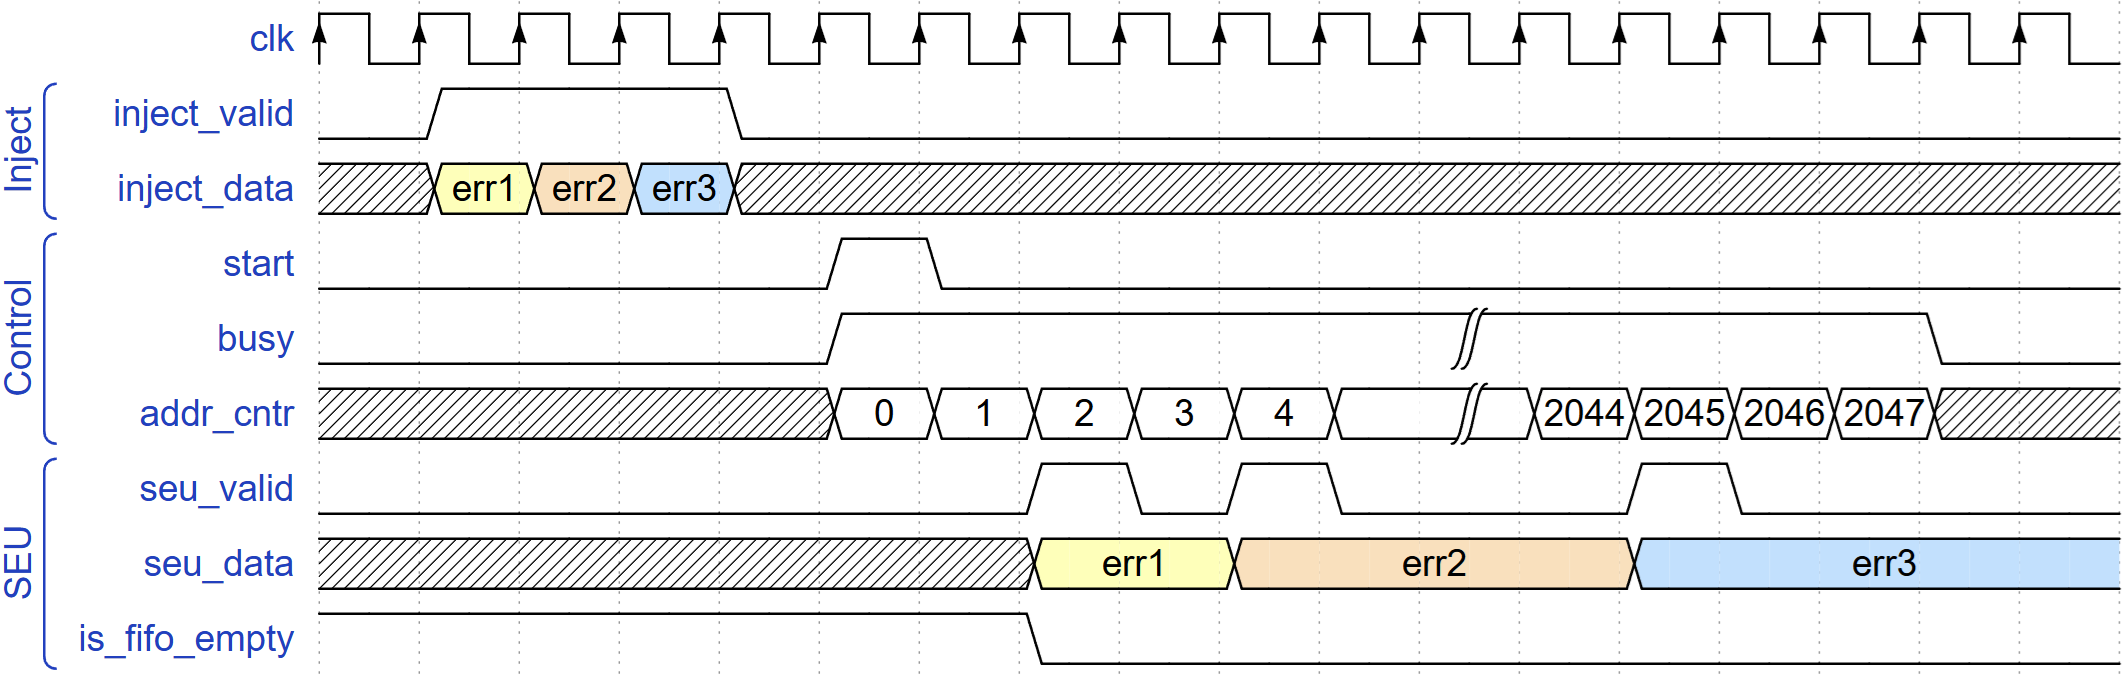
\includegraphics[width=\columnwidth]{./Images/sw_de_waveforms.png}
    \caption{Formele de undă ce exemplifică funcționarea modulului DU.}%
\label{fig:sw_de_waveforms}
\end{figure}

\subsection{Detector Element (DE)}
Modulul \acrfull{de} este alcătuit din trei componente principale: un contor de adrese protejat prin \gls{tmr}, o unitate de memorie (realizată fie cu \gls{bram}, fie cu \gls{lutram}) și modulul de monitorizare (Monitor), responsabil cu detecția erorilor de tip bit-flip. Diagrama acestui modul este prezentată în Figura~\ref{fig:sw_de_general_diagram} și este similară cu cea propusă în~\cite{isetc}, cu excepția integrării logicii de inserare a erorilor. La activarea semnalului START, contorul \gls{tmr} începe să incrementeze valoarea adresei, care este transmisă simultan către portul B al memoriei și către modulul Monitor. În timpul procesului de scanare, dacă se detectează neconcordanțe între registrele din sistemele \gls{tmr} (în contor sau în Monitor), semnalul SEU\_LOGIC este activat. Acesta se obține dintr-o poartă OR aplicată asupra semnalelor provenite de la fiecare registru protejat, iar rezultatul este stocat într-un registru, pentru a putea fi transmis odată cu primul \gls{seu} detectat.

Modulul Monitor, având la dispoziție atât adresa memoriei, cât și valoarea de la adresa respectivă, poate determina dacă a avut loc un bit-flip cauzat de \gls{seu}, printr-un set de operații logice simple. În cazul afirmativ, se activează semnalul SEU\_VALID și sunt transmise semnalele relevante prin firele SEU.\@ Concomitent, valoarea afectată din memorie este corectată prin portul A, folosind adresa curentă și valoarea așteptată (aleasă în funcție de paritatea adresei).

\begin{figure}[h!]
    \centering
    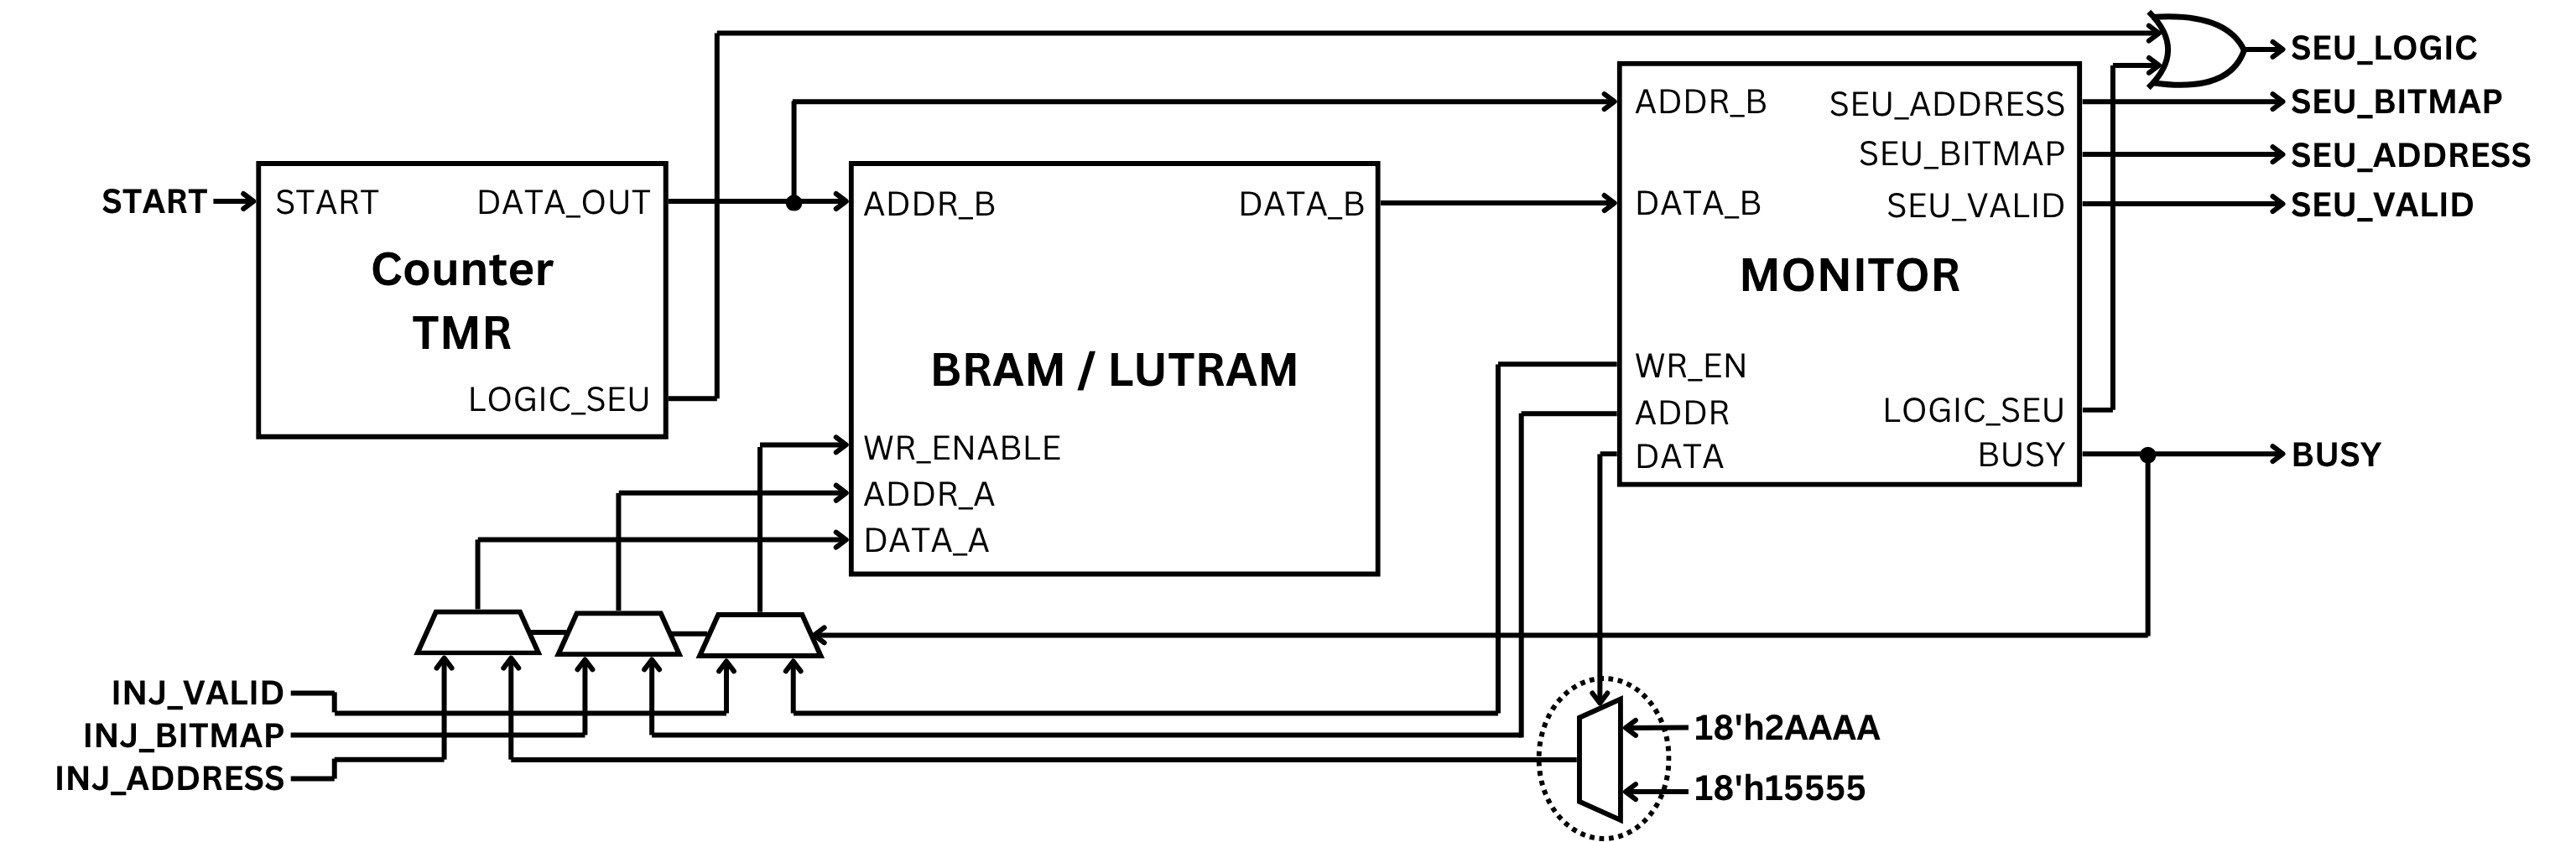
\includegraphics[width=\columnwidth]{./Images/sw_de_general_diagram.png}
    \caption{Schema bloc a modulului Detector Element (DE).}%
\label{fig:sw_de_general_diagram}
\end{figure}

Inserarea erorilor se face tot prin portul A al memoriei, dar numai atunci când modulul \gls{de} nu se află într-un ciclu de scanare. Dacă semnalul BUSY este \enquote{1}, cele trei multiplexoare din colțul stânga jos al diagramei selectează semnalele provenite din modulul Monitor, care are prioritate pentru a corecta eventualele erori detectate în timpul scanării. În schimb, dacă semnalul BUSY este \enquote{0}, aceleași multiplexoare aleg semnalele INJ, permițând scrierea intenționată a unor valori eronate în memorie.

\subsection{LUTRAM}%
\label{lutram}
După cum s-a menționat anterior, memoriile de tip \gls{bram} nu reprezintă singurele structuri dintr-un \gls{fpga} capabile să stocheze date. Pe lângă acestea, AMD oferă posibilitatea generării automate a blocurilor \gls{fifo} (acestea utilizând însă tot \gls{bram}-uri~\cite{ug473}), iar dispozitivele din familiile UltraScale și UltraScale+ dispun și de memorie \gls{uram}. De asemenea, \gls{ff}-urile prezente în număr mare pot reține valori, dar capacitatea lor este prea mică, iar utilizarea lor pentru stocare ar crește semnificativ complexitatea unei implementări, fără un câștig proporțional în performanța senzorului. Cea mai bună alternativă la memoria \gls{bram} rămâne memoria distribuită \gls{lutram}.

În arhitectura hardware, un \acrfull{lut} reprezintă o simplificare a implementării funcțiilor logice prin pre-calcularea rezultatelor posibile și stocarea acestora într-un tabel de adevăr. În funcție de intrare, \gls{lut}-ul oferă valoarea de ieșire corespunzătoare, rapid și cu o latență redusă. În majoritatea \gls{fpga}-urilor moderne, \gls{lut}-urile sunt construite cu celule \gls{sram}, celule care pot fi reutilizate pentru implementarea unor memorii \gls{ram} de dimensiuni mici cu o latență foarte scăzută. Denumirea de memorie distribuită provine din faptul că aceste celule \gls{lut}-uri sunt dispersate relativ uniform în întregul dispozitiv \gls{fpga}.

AMD pune la dispoziție mai multe primitive \gls{lutram} de dimensiuni și tipuri variate~\cite{ug953}. În cadrul acestui proiect, a fost aleasă primitiva RAM128X1D, o memorie \gls{ram} de 128 de adrese pe un singur bit. Deși există și primitive cu o capacitate mai mare (256 de valori), RAM128X1D a fost aleasă datorită interfeței dual-port necesară pentru a replica fidel comportamentul unei memorii \gls{bram}. Pentru a ajunge la dimensiuni comparabile cu cele ale unui \gls{bram}, sunt concatenate mai multe primitive \gls{lutram} atât în serie, cât și în paralel, obținându-se astfel o memorie mai mare și mai ușor de integrat în locul unui \gls{bram} standard.

O variantă simplificată a codului sursă utilizat pentru generarea unei memorii cu dimensiuni parametrizabile, având aceeași interfață ca un \gls{bram} dual-port, este prezentată în Figura~\ref{fig:sw_lutram_code}. Codul conține două bucle for: prima buclă instanțiază primitivele în serie, crescând spațiul de adrese, iar a doua în paralel, crescând lățimea cuvântului. Alegerea atentă a intervalelor de biți (la liniile 23, 25 și 28) asigură implementarea corectă a logicii de multiplexare necesară pentru conectarea instanțelor \gls{lutram}. Pentru a imita cu acuratețe un \gls{bram}, au fost introduși regiștrii de pipeline pentru ieșire, iar valorile de inițializare (INIT) sunt setate prin folosirea parametrilor INIT\_A și INIT\_B, reglați pentru a genera secvențele binare alternante \enquote{1}-\enquote{0} sau \enquote{0}-\enquote{1}.

\begin{figure}[h!]
\begin{lstlisting}[language=Verilog]
module lut_ram #(
    parameter WIDTH =           18     ,
    parameter DEPTH =           2048   ,
) (
    input                       clka   ,                      
    input                       wea    ,   
    input [$clog2(DEPTH)-1 : 0] addra  , 
    input [WIDTH-1 : 0]         dina   ,                 
    input [$clog2(DEPTH)-1 : 0] addrb  ,  
    output [WIDTH-1 : 0]        doutb
);

wire [WIDTH-1 : 0] read_data [(DEPTH/128)-1 : 0];
assign doutb <=    read_data [addrb_d];

generate
    for (j = 0; j < DEPTH/128; j = j + 1) begin : gen_bank
        for (i = 0; i < WIDTH; i = i + 1) begin : gen_lutram
        RAM128X1D #(
           .INIT    ({64{INIT_B[i], INIT_A[i]}})
        ) RAM128X1D_inst (
           .WCLK    (clka                                   ), 
           .WE      (wea & (addra[$clog2(DEPTH)-1 : 7] == j)),
           .A       (addra[7-1 : 0]                         ),        
           .D       (dina[i]                                ),    
           .SPO     (                                       ),
           .DPRA    (addrb[7-1 : 0]                         ),  
           .DPO     (read_data[j][i]                        )       
        );
        end
    end
endgenerate
endmodule
\end{lstlisting}
\caption{Codul simplificat al modulului care instanțiază primitivele LUTRAM.}%
\label{fig:sw_lutram_code}
\end{figure}

Acest modul a fost supus simulării pentru a confirma comportamentul dorit, iar ulterior a fost sintetizat și implementat. Resursele logice utilizate pentru o instanță a modulului sunt prezentate în Tabelul~\ref{tab:sw_lutram_utilization}. După cum se poate deduce și analitic, numărul de \gls{lutram}-uri utilizate este 1152, rezultat din înmulțirea a 16 memorii în serie, 18 în paralel și 4 memorii pentru fiecare instanță de 128 de adrese. Numărul ridicat de multiplexoare este justificat de necesitatea concatenării instanțelor \gls{lutram}, însă, având în vedere că restul proiectului utilizează un număr redus de multiplexoare, acest aspect nu ar trebui să afecteze scalabilitatea proiectului.

\begin{table}[h!]
  \centering
  \renewcommand{\arraystretch}{1.3}
  \caption{Utilizarea resurselor pentru o instanță a modulului LUTRAM.}%
  \label{tab:sw_lutram_utilization}
  \begin{tabular}{L{4cm} C{2.05cm} C{2.05cm} C{2.05cm} C{2.05cm} C{2.05cm}}
    \toprule
    \textbf{Tip} & \textbf{FF-uri} & \textbf{LUT-uri} & \textbf{LUTRAM} & \textbf{Muxuri F7} & \textbf{Muxuri F8}\\
    \midrule
        \textbf{Disponibile pe FPGA} & 269200 & 134600 & 46200 & 67300 & 33650 \\
        \textbf{Modulul LUTRAM} & 40 & 80 & 1152 & 612 & 18 \\
    \bottomrule
  \end{tabular}
\end{table}

Numărul maxim de module se determină prin împărțirea numărului total de resurse de tip \gls{lutram} disponibile la numărul de \gls{lutram}-uri necesare pentru o instanță. În urma acestui calcul, rezultă 40 de blocuri de dimensiuni echivalente cu cele \gls{bram}, ce pot fi inserate direct în locul modulelor \gls{bram} pentru a crește numărul de elemente de detecție a radiației. Totuși, folosirea intensă a memoriei distribuite impune o provocare semnificativă uneltelor de sintetizare și implementare, care nu reușesc să respecte constrângerile de tip hold. Această limitare a fost depășită prin aplicarea unei strategii alternative de sintetizare, denumită Flow\_AlternateRoutability, ce utilizează un set optimizat de algoritmi pentru eficientizarea rutabilității și pentru reducerea numărului de multiplexoare utilizate~\cite{ug901}.

\section{Tehnici de protecție împotriva radiației}
Problema implementării unui senzor de radiație folosind un dispozitiv \gls{fpga} constă chiar în caracteristica esențială care permite realizarea acestuia: sensibilitatea la radiație. Acest \enquote{avantaj și dezavantaj} determină apariția de erori de tip \gls{seu} nu doar în memoriile de detecție, unde sunt intenționate și utile, ci și în restul elementelor logice ale dispozitivului, de la registre individuale \gls{ff}, până la memoria de configurare a \gls{fpga}-ului. Din acest motiv, apare nevoia utilizării unor tehnici adiționale de protecție pentru acele circuite și componente în care un bit-flip compromite funcționarea corectă a sistemului.

Tehnicile discutate în acest capitol acoperă mai multe niveluri: de la protejarea componentelor individuale, precum memoria \gls{cram} sau registrele, la metode generale de protecție împotriva erorilor, cum ar fi \gls{ecc} și \gls{crc}, până la strategii de protejare a întregului dispozitiv \gls{fpga}, prin reprogramarea acestuia cu un proiect redundant, în cazul unei configurații compromise.

\subsection{Protejarea memoriei de configurare a FPGA-ului}%
\label{sem}
\gls{ip}-ul oferit de AMD pentru monitorizarea și corectarea erorilor apărute în memoria de configurare a dispozitivelor \gls{fpga} poartă denumirea \acrfull{sem}~\cite{pg036}. În cadrul proiectului de față, acest modul a fost utilizat în paralel cu blocul \gls{du}, cu scopul de a extinde zona sensibilă a detectorului (și implicit, performanța) și de a crește fiabilitatea dispozitivului prin protejarea memoriei \gls{cram}.\@ \gls{ip}-ul \gls{sem} reprezintă doar blocul de control, responsabil cu gestionarea datelor primite de la două primitive externe. Pentru buna lui funcționare, acesta a fost încapsulat într-un modul ajutător care implementează aceste primitive și oferă o interfață simplificată, care poate fi integrată mai ușor în restul proiectului.

Principalele primitive utilizate în combinație cu controller-ul \gls{sem} sunt ICAP și FRAME\_ECC, fiecare având o interfață dedicată pe controller. Primitiva ICAP permite accesul utilizatorului la registrele și circuitele de configurare ale \gls{fpga}-ului, iar FRAME\_ECC monitorizează automat circuitele de corecție de erori \gls{ecc} și \gls{crc} din memoria de configurare.\@ \gls{cram}-ul este structurat într-o matrice de frame-uri, fiecare cu un cod \gls{ecc},  în timp ce întregul ansamblu este protejat de un cod global \gls{crc}. În combinație, aceste primitive permit identificarea erorilor apărute la anumite coordonate din memoria \gls{cram} și corectarea lor prin modificarea valorilor stocate, un mecanism similar cu cel utilizat în modulul \gls{du} pentru corectarea erorilor din \gls{bram}-uri.

Interfața modulului rezultat este prezentată în Figura~\ref{fig:sw_sem_interface_code}. Aceasta conține cele trei semnale de ceas identice (folosite pentru sistemele \gls{tmr}), un semnal de reset,  un contor pe 16 biți al erorilor identificate de la pornirea sistemului, o interfață de monitorizare (\textit{status}) și una pentru inserare de erori (\textit{inject}). Controller-ul \gls{sem} funcționează ca o mașină de stări finite, indicând starea curentă prin activarea unuia dintre semnalele \textit{status}, cu excepția semnalului \textit{status\_heartbeat}, care generează impulsuri periodice în timpul stării de monitorizare. Acesta poate fi folosit în implementarea unui watchdog timer, pentru a verifica dacă \gls{ip}-ul funcționează corect și dacă se află în starea activă de operare.

Interfața inject oferă o metodă de comunicație rudimentară ce permite controlul direct al primitivei ICAP și inserarea manuală de erori în memoria \gls{cram}. Pe lângă aceasta, mai există interfața monitor, bazată pe protocolul \gls{uart}, care permite o metodă mai robustă de a comunica cu modulul \gls{sem}. Aceasta a fost însă exclusă pentru a reduce complexitatea modulului și din cauza lipsei unei interfețe \gls{uart} robuste pe nanosatelit.

Interfața inject utilizează semnalul \textit{inject\_address}, cu o lățime de 40 de biți, pentru trimiterea comenzilor dorite, și \textit{inject\_strobe} pentru confirmarea trimiterii unei comenzi. Prin această interfață se pot trimite două tipuri de comenzi: schimbarea stării mașinii de stări finite (prin codarea celor mai semnificativi patru biți ai adresei) sau inserarea de erori specifice, prin specificarea coordonatelor frame-ului, cuvântului și bitului afectat. În plus, semnalul \textit{inject\_forced\_start} a fost introdus pentru a readuce controller-ul în starea de monitorizare în urma unei erori necorectabile (acesta întrerupând scanarea în cazul unei astfel de erori).

\begin{figure}[ht!]
\begin{lstlisting}[language=Verilog]
module sem_wrapper(
  input         clk_iA                ,
  input         clk_iB                ,
  input         clk_iC                ,
  input         reset_i               ,
  
  output        status_heartbeat      ,
  output        status_initialization ,
  output        status_observation    ,
  output        status_correction     ,
  output        status_classification ,
  output        status_injection      ,
  output        status_essential      ,
  output        status_uncorrectable  ,
  
  output [15:0] error_counter         ,
  
  input         inject_strobe         ,
  input [39:0]  inject_address        ,
  input         inject_forced_start
);
\end{lstlisting}
\caption{Interfața modulului Verilog SEM.}%
\label{fig:sw_sem_interface_code}
\end{figure}

Diagrama de stări și tranziții a acestui modul este ilustrată în Figura~\ref{fig:sw_sem_fsm}, evidențiind relația dintre diferitele stări ale mașinii de stări finite. Se observă că modulul trece printr-o fază de inițializare, unde se aduce într-o stare cunoscută, urmată automat de trecerea în starea \textit{observation}, în care se realizează scanarea continuă a memoriei \gls{cram}. La detectarea unei erori, \gls{ip}-ul  \gls{sem} trece obligatoriu prin stările de \textit{correction} și \textit{classification}, indiferent dacă aceste opțiuni au fost selectate ca funcționalități la crearea \gls{ip}-ului. Tranziția prin starea \textit{correction} la fiecare eroare detectată este utilizată și pentru incrementarea contorului \textit{error\_counter}. Acest comportament este independent de natura erorii, fie ea corectabilă sau necorectabilă, ceea ce permite o contorizare robustă a \gls{seu}-urilor apărute. După starea \textit{classification}, în funcție de tipul erorii detectate, se activează semnalul \textit{essential} dacă eroarea afectează o zonă utilizată a memoriei de configurare, respectiv semnalul \textit{uncorrectable}, în cazul în care eroarea a fost identificată, dar nu poate fi corectată din anumite motive.

\begin{figure}[h!]
    \centering
    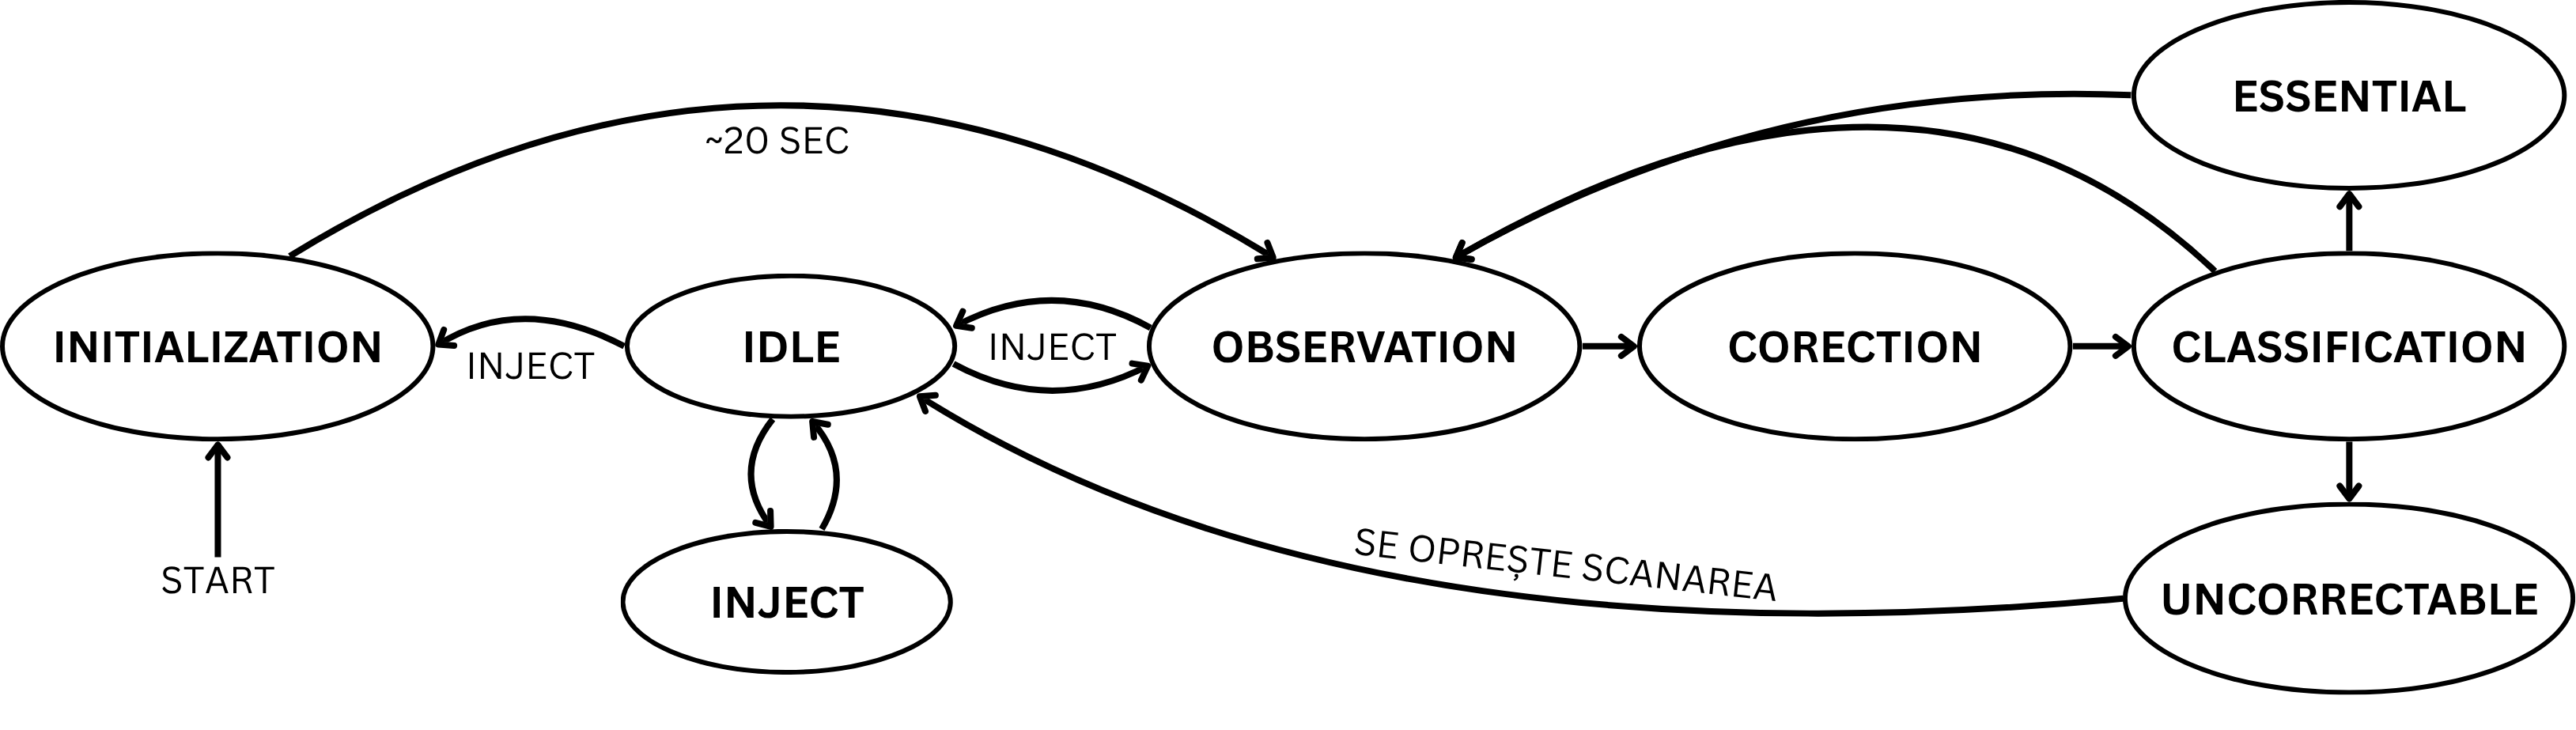
\includegraphics[width=\columnwidth]{./Images/sw_sem_fsm.png}
    \caption{Diagrama de stări și tranziții a IP-ului SEM.}%
\label{fig:sw_sem_fsm}
\end{figure}

Din această Figură reiese că, în cazul identificării unei erori necorectabile, controller-ul iese din starea de scanare automată și intră în starea \textit{idle}, unde rămâne blocat până la reinițializarea modulului și corectarea erorii, sau până la primirea unei comenzi specifice pe interfața inject. Pentru a evita această întrerupere, a fost introdus semnalul suplimentar \textit{inject\_forced\_start}, care forțează trecerea din starea \textit{idle} în starea \textit{observation}, reluând astfel scanarea. 

La crearea \gls{ip}-ului pot fi alese mai multe setări și funcționalități diferite, în funcție de scopurile proiectului. Au fost selectate opțiunile de injectare și corectare de erori, iar frecvența de operare a fost aliniată cu cea a restului sistemului. Metoda de corecție de erori aleasă a fost \textit{Enhanced Repair}, care combină codurile \gls{ecc} și \gls{crc} pentru a putea detecta două erori și a corecta una. Deși există o variantă superioară, \textit{Replace}, care presupune înlocuirea frame-ului corupt cu o copie stocată extern, aceasta a fost exclusă din lipsa unei memorii redundante. În final, resursele utilizate de acest modul includ 8.5 memorii \gls{bram} și 26 de memorii \gls{lutram}, un preț mic de plătit în raport cu avantajele semnificative aduse în ceea ce privește integritatea și eficiența sistemului.

\subsection{Triple Modular Redundancy (TMR)}%
\label{tmr}
Conceptul de \gls{tmr} a fost introdus de Von Neumann în~\cite{neumann_book_tmr}, unde propune utilizarea unui \enquote{organ de majoritate} care, pe baza a trei semnale provenite din surse logice identice, identifică și corectează eventualele erori apărute pe una dintre ramuri, îmbunătățind astfel fiabilitatea generală a sistemului. Această idee a fost extinsă semnificativ de IBM în~\cite{ibm_paper_tmr}, prin implementarea practică a unui circuit de vot majoritar combinațional, cu cele trei intrări provenite din elemente secvențiale redundante. Autorii concluzionează că \gls{tmr} este o metodă excelentă de creștere a fiabilității prin redundanță logică, atâta timp cât este utilizată cu moderație și nu înlocuiește complet alte tehnici de detectare și corectare a erorilor.

În cadrul acestui proiect, noțiunea de \gls{tmr} a fost implementată prin realizarea a două module similare: TMR\_register și TMR\_register\_simple, codul simplificat al celui din urmă fiind ilustrat în Figura~\ref{fig:sw_tmr_register_code}. Diferența dintre cele două constă în prezența unui reset sincron configurabil în modulul TMR\_register, în plus față de reset-ul asincron, prezent în ambele variante. Aceste module au fost utilizate oriunde a fost necesară implementarea unui registru, iar semnalele de detecție a erorilor generate de aceste module au fost concatenate printr-o poartă OR și memorate într-un pachet de date din modulul \gls{du}.

Ideea generală constă în replicarea unui registru în trei instanțe identice, fiecare având același semnal de intrare, semnal de activare și semnal de reset, dar având ceasuri diferite. Ieșirile celor trei registre sunt evaluate de două circuite de vot majoritar: unul pentru selectarea semnalului de ieșire (activ dacă cel puțin două dintre registre conțin aceeași valoare --- linia 32), iar celălalt pentru detectarea unei posibile erori, prin identificarea unei diferențe între cele trei semnale (linia 33). Pentru a preveni optimizarea automată a acestor registre de către unealta de sintetizare, fiecare \gls{ff} este protejat prin atributul \textit{DONT\_TOUCH=\enquote{true}}, iar blocul \textit{generate} este necesar datorită creării de \gls{ff}-uri diferite în funcție de frontul semnalului de reset.

\begin{figure}[ht!]
\begin{lstlisting}[language=Verilog]
(* DONT_TOUCH=\enquote{true} *) reg[SIGNAL_WIDTH - 1 : 0] sgn_A;
(* DONT_TOUCH=\enquote{true} *) reg[SIGNAL_WIDTH - 1 : 0] sgn_B;
(* DONT_TOUCH=\enquote{true} *) reg[SIGNAL_WIDTH - 1 : 0] sgn_C;

generate
    always @(posedge clk_iA or posedge reset_i) begin 
        if (reset_i)
            sgn_A <= #TP {SIGNAL_WIDTH {1'b0}};
        else if (true_condition_i)
            sgn_A <= #TP signal_in;
        else
            sgn_A <= #TP signal_out;
    end  
    always @(posedge clk_iB or posedge reset_i) begin
        if (reset_i)
            sgn_B <= #TP {SIGNAL_WIDTH {1'b0}};
        else if (true_condition_i)
            sgn_B <= #TP signal_in;
        else
            sgn_B <= #TP signal_out;
    end  
    always @(posedge clk_iC or posedge reset_i) begin
        if (reset_i)
            sgn_C <= #TP {SIGNAL_WIDTH {1'b0}};
        else if (true_condition_i)
            sgn_C <= #TP signal_in;
        else
            sgn_C <= #TP signal_out;
    end
endgenerate

signal_o = (sgn_B & sgn_A) | (sgn_A & sgn_C) | (sgn_C & sgn_B);
seu_o = (~sgn_B & sgn_A) | (~sgn_A & sgn_C) | (~sgn_C & sgn_B);
\end{lstlisting}
\caption{Conținutul simplificat al modulului Verilog TMR\_register\_simple.}%
\label{fig:sw_tmr_register_code}
\end{figure}

Modulele rezultate au la fel de multe intrări și ieșiri ca un registru standard, menținând un nivel mare de flexibilitate. Acestea includ trei parametri pentru a configura aspecte ca: frontul activ al semnalului de reset, lățimea semnalului de date și o valoare de reset configurabilă, disponibilă în modulul mai avansat. Logica combinațională necesară este implementată eficient prin două \gls{lut}-uri (pentru un semnal de intrare de un bit) și este ușor scalabilă, iar numărul de \gls{ff}-uri, deși triplu față de un registru normal, crește liniar cu dimensiunea semnalului de date. Variante de redundanță extinsă, cu cinci sau șapte elemente logice, au fost luate în considerare, dar au fost considerate prea costisitoare pentru avantajele marginale aduse.

\subsection{Coduri detectoare sau corectare de erori}
Prima mențiune a unor astfel de coduri \gls{ecc} în logica digitală a fost făcută de Richard Hamming în~\cite{hamming_book_ecc}, unde propune inserarea unor biți de paritate în poziții specifice ale unui cuvânt (la puteri ale lui 2), pentru a permite detectarea și corectarea erorilor de un singur bit. Mai târziu, acest cod Hamming a fost extins în varianta \gls{secded} prin adăugarea unui bit global de paritate la finalul cuvântului, permițând astfel corectarea unei erori și detectarea a două erori. Pentru acest proiect, a fost utilizată această variantă extinsă, în situațiile în care era necesară o metodă adițională de protejare pe lângă \gls{tmr}. Codurile \gls{crc} au fost considerate, dar neavând abilitatea de a corecta erori, nu au fost implementate activ, ci au fost utilizate sub forma instanțelor deja integrate în \gls{fpga} (în memoria \gls{cram} și în funcționalitatea \gls{fpga} MultiBoot). Alte tipuri avansate de coduri \gls{ecc}, precum cele BCH, Reed-Solomon sau Turbo, nu au fost luate în considerare din cauza complexității ridicate și a gradului de protecție exagerat pentru aplicația curentă.

Principalele locuri unde codul \gls{ecc} a fost folosit sunt în cadrul \gls{fifo}-urilor și în procesul de transmitere a pachetelor de date către \gls{obc}. Pentru a evita implementarea unei logici separate pentru fiecare instanță de utilizare a acestor coduri, s-a optat pentru utilizarea \gls{ip}-ului \gls{ecc} oferit de AMD, care implementează automat logica de codare sau decodare \gls{secded}, pentru orice lățime a cuvântului între 4 și 64 de biți. Numărul minim de biți de paritate este determinat automat folosind relația \(2^r \geq n + r + 1\), unde \textit{r} este numărul de biți de paritate Hamming, iar \textit{n} reprezintă numărul de biți de date, cu un bit suplimentar adăugat la final.

Deoarece triplicarea unui întreg \gls{fifo} ar fi prea costisitoare, s-a ales codificarea datelor la intrare și decodificarea acestora la ieșire, înainte de a fi transmise mai departe. Astfel se asigură protejarea pe întreaga durată de stocare a datelor și se creează semnale de indicare a erorilor, care pot fi concatenate cu semnalele SEU\_LOGIC descrise anterior. De asemenea, deoarece pachetele de date transmise către \gls{obc} conțin anumite spații libere, utilizate pentru alinierea datelor la multipli de 8 biți (structura pachetelor fiind descrisă în Capitolul~\ref{spi}), se pot introduce coduri checksum pentru valorile individuale din aceste pachete, oferind un strat adițional de protecție în timpul transmisiei. Codificarea este realizată pe \gls{fpga} cu ajutorul unui algoritm XOR, iar decodificarea este efectuată pe \gls{obc} de către microprocesorul principal, printr-un algoritm scris în C.

\subsection{FPGA MultiBoot}
Pentru anumite interfețe de configurare ale unui \gls{fpga} Xilinx, precum \gls{spi} folosit în cadrul acestui proiect, poate fi activată o funcționalitate specială care permite \gls{fpga}-ul să încarce un nou fișier de configurare în cazul în care cel inițial devine corupt. Acest mecanism, denumit MultiBoot, se bazează pe detecția erorilor prin codurile \gls{crc} integrate în fiecare fișier bitstream și se activează prin adăugarea unor comenzi specifice în fișierul de constrângeri ale proiectului~\cite{xapp1247}. De obicei, MultiBoot este folosit pentru a asigura existența unui proiect de rezervă, cunoscut ca fiind funcțional, care poate fi încărcat în cazul în care bitstream-ul principal conține erori de implementare sau funcționale. Totodată, această funcționalitate este relevantă și în contextul protecției împotriva radiației cosmice, care poate corupe configurația \gls{fpga}-ului.

Procesul presupune generarea a două fișiere bitstream identice, dintre care unul conține opțiunile suplimentare BITSTREAM.\allowbreak\ CONFIG.\allowbreak\ CONFIGFALLBACK, care activează funcția MultiBoot, și BITSTREAM.\allowbreak\ CONFIG.\allowbreak\ NEXT\_\allowbreak\ CONFIG\_\allowbreak\ ADDR care indică adresa din memoria externă unde este stocat bitstream-ul de rezervă. Ulterior, se execută o comandă tcl specială, care combină cele două bitstream-uri într-un singur fișier binar pentru programarea cipului de memorie. În urma acestei comenzi, bitstream-ul principal este plasat la adresa 0, iar cel de rezervă la adresa specificată, restul memoriei fiind umplut cu valori nule. 

În momentul pornirii, \gls{fpga}-ul începe configurarea cu bitstream-ul de la adresa 0. Dacă este detectată o eroare \gls{crc}, se face trecerea la bitstream-ul de rezervă. O opțiune suplimentară care reduce șansele de apariție a unor erori este BITSTREAM.\allowbreak\ GENERAL.\allowbreak\ COMPRESS, care comprimă fișierele de configurare de până la zece ori. Un fișier mai mic reduce probabilitatea ca o particulă cosmică să altereze un bit important. Aceste metode au fost testate cu succes pe \gls{fpga}, trecerea la bitstream-ul de rezervă fiind realizată prin coruperea deliberată a fișierului principal.

\section{Modulele de comunicație}
Dispozitivul \gls{fpga} detaliat în capitolele anterioare are, pe lângă funcționalitatea principală de a detecta bit-flip-uri cauzate de \gls{seu}-uri, și rolul de a comunica și monitoriza alte componente, aflate atât pe plăcuța \gls{aicors}, cât și pe \gls{pcb}-ul cu \gls{obc}. Pentru a îndeplini această funcție, au fost dezvoltate și implementate mai multe module Verilog care asigură compatibilitate cu diferite protocoale de comunicație, necesare interacțiunii cu fiecare dispozitiv în parte. Principalele interfețe vizate sunt: \gls{uart}, folosită de modulul \gls{sem} pentru raportarea erorilor detectate, \gls{i2c}, pentru monitorizarea senzorilor de curent de pe \gls{pcb}, și \gls{lvds} \gls{spi}, responsabilă de transmiterea pachetelor de date relevante către \gls{obc}. Aceste module vor fi prezentate și analizate în capitolele următoare, cu excepția modulului \gls{uart}, care nu a mai fost integrat în versiunea finală a proiectului.

Modulul \gls{uart} implementa cele două canale de comunicație (transmisie și recepție) prin intermediul a două registre de shiftare, completate cu logică auxiliară și mai multe setări parametrizabile, precum: tipul de paritate, frecvența de ceas de intrare, frecvența de transmisie, ordinea biților în cadrul cuvântului transmis și dimensiunea filtrului de zgomot aplicat datelor de intrare. Acest modul a fost conectat la interfața Monitor a blocului \gls{sem}, prezentat în Capitolul~\ref{sem}, pentru testarea funcționalității acestuia. Cu toate acestea, având în vedere absența unei interfețe \gls{uart} între \gls{fpga} și \gls{obc}, interfața Monitor nu a mai fost utilizată, iar modulul \gls{uart} nu a fost inclus în configurația finală și, prin urmare, nu va fi detaliat în continuare.

\subsection[Inter-Integrated Circuit (I2C)]{Inter-Integrated Circuit (I\textsuperscript{2}C)}
Protocolul \gls{i2c}, patentat inițial de NXP Semiconductors~\cite{patent_i2c}, este o interfață serială de comunicație cu două fire, unul de ceas (SCL) și unul de date (SDA), folosită pentru transmisii de viteză redusă între un procesor și circuite integrate auxiliare. Viteza maximă de transmisie a datelor este limitată la 5 Mb/s din cauza naturii open-drain a liniilor SCL și SDA, care, deși oferă robustețe, nu permit un timp de creștere suficient de rapid din cauza constantei de timp RC asociate capacității parazite a \gls{pcb}-ului și a rezistenței de pull-up de pe fiecare linie. Pe o magistrală \gls{i2c} există un singur dispozitiv de control, denumit master, și mai multe dispozitive auxiliare (slave), fiecare identificabil printr-o adresă unică. În multe cazuri, aceste adrese pot fi setate prin conectarea unor pini speciali la VCC sau la GND.\@ În cadrul proiectului, acest protocol este utilizat de patru senzori de curent INA219, prezenți pe \gls{pcb}-ul \gls{aicors}, dar și cu un \gls{io} Expander integrat pe a doua versiune a plăcii, care conectează diferite semnale de status la \gls{fpga}.

Modulul dezvoltat are rol de master și este bazat pe o mașină de stări finite (FSM) care controlează secvența necesară pentru transmiterea unui pachet de date \gls{i2c}. Formele de undă asociate unui astfel de pachet sunt prezentate în Figura~\ref{fig:sw_i2c_waveforms}, iar diagrama de stări a FSM-ului este ilustrată în Figura~\ref{fig:sw_i2c_fsm}. Interfața modulului include o pereche de trei semnale pentru controlul celor două \gls{fifo}-uri de la intrare și ieșire, precum și cele două linii specifice protocolului \gls{i2c}, direcționate către doi pini \gls{io} ai \gls{fpga}-ului. Aceste semnale sunt transmise prin două buffere tri-state, pentru a implementa starea de înaltă impedanță caracteristică magistralei \gls{i2c}. Modulul integrează și logica de arbitrare, esențială pentru a da controlul magistralei unui singur dispozitiv și pentru a-i permite să comunice, în funcție de ordinea inițierii transmisiunii.

FSM-ul menționat conține patru stări principale: \textit{LD\_ADDR}, care încarcă adresa dispozitivului țintă și un bit care indică tipul tranzacției curente ca una de citire sau scriere. \textit{RD\_DATA} și \textit{WR\_DATA} realizează citirea sau scrierea de date în funcție de bitul de comandă, iar \textit{ACK\_NACK}, intermediar între celelalte stări, gestionează semnalele de Acknowledge și Not Acknowledge, care sunt de lățimea unui bit și care provin de la dispozitivul care transmite date la momentul respectiv. Există câte un semnal ACK după adresă și după fiecare opt biți transmiși, pentru a asigura că dispozitivul receptor este prezent și primește mesajele, iar odată ce se întâlnește un semnal NACK, tranzacția se oprește. Pe lângă acestea, stările IDLE, START și STOP asigură tranzițiile corecte în parcurgerea FSM-ului, iar starea WAIT a fost introdusă pentru a preveni inițierea unei noi tranzacții în cazul în care o transmisie este deja în curs sau dacă s-a detectat o coliziune pe magistrală.

\vspace{0.7em}
\begin{figure}[h!]
    \centering
    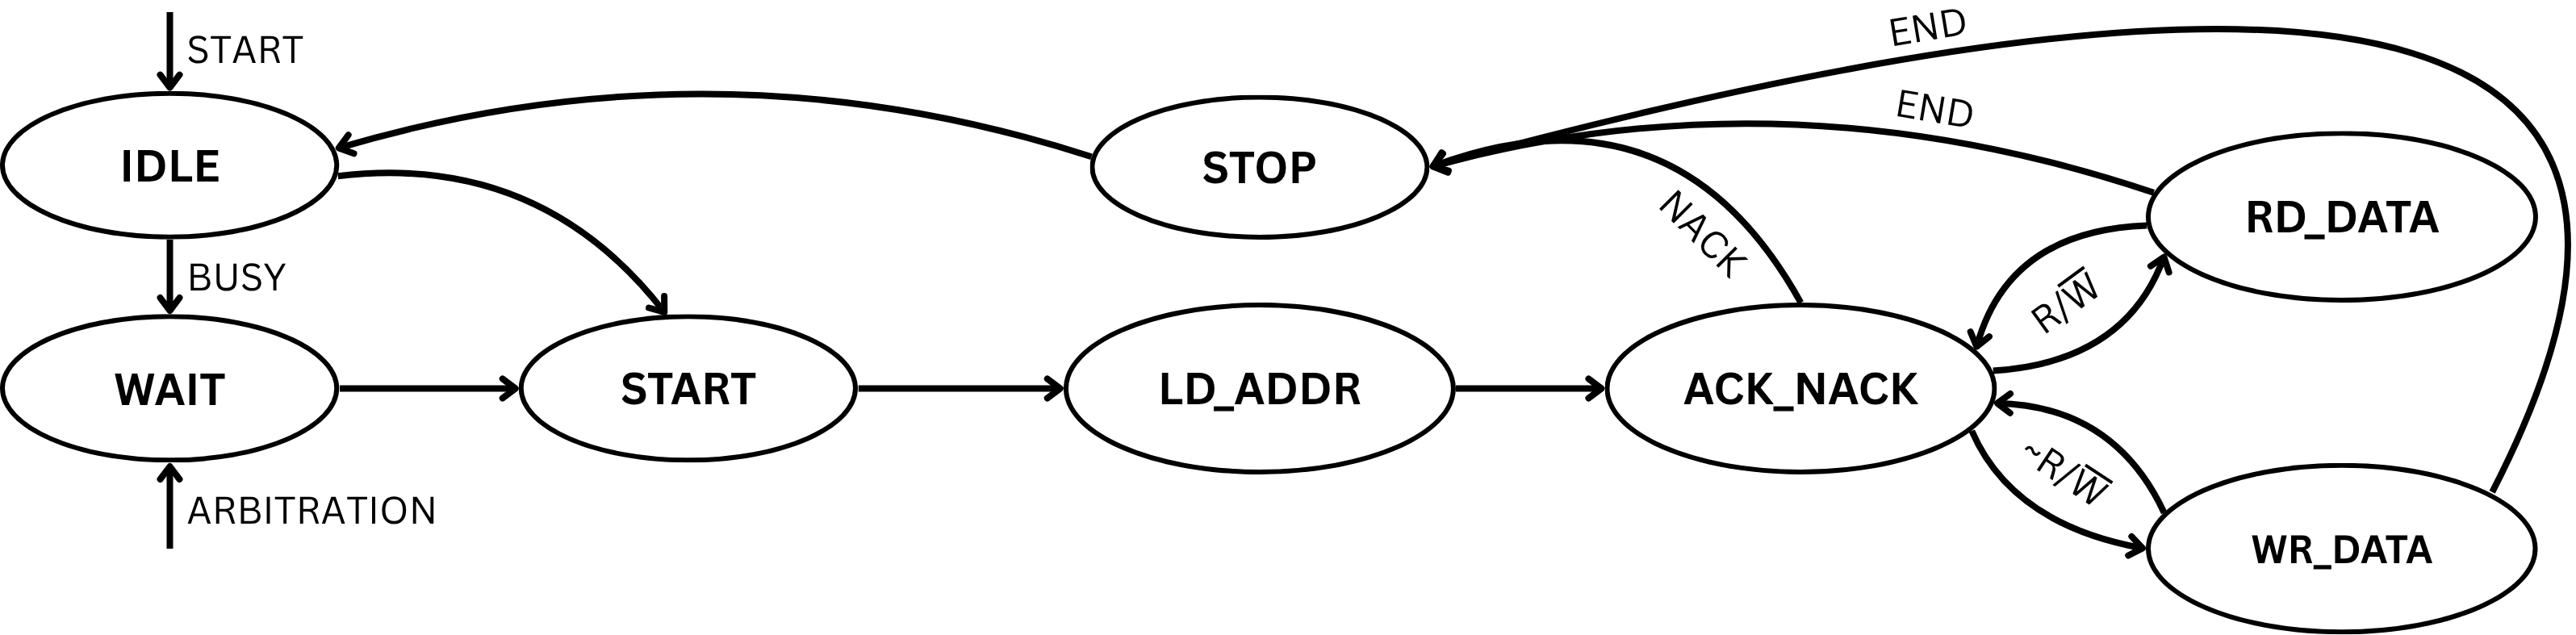
\includegraphics[width=\columnwidth]{./Images/sw_i2c_fsm.png}
    \caption{Diagrama de stări și tranziții a modulului I2C.}%
\label{fig:sw_i2c_fsm}
\end{figure}

Formele de undă care asociază stările FSM-ului cu etapele unei transmisii \gls{i2c} sunt prezente în partea de sus a Figurii~\ref{fig:sw_i2c_waveforms}. Se observă starea IDLE cât timp nu există activitate pe magistrală, START, inițiat prin coborârea semnalului SDA înainte de SCL, și STOP prin ridicarea lui SCL înainte de SDA.\@ În cadrul stării LD\_ADDR se transmit cei 7 biți de adresă (sau opțional 10 biți de adresă, configurabil printr-un parametru din modul), urmați de bitul R/$\overline{\mbox{W}}$. După fiecare octet transmis urmează starea ACK/NACK, pentru confirmarea recepției. De asemenea, se mai poate observa că semnalul de ceas este evaluat pe frontul negativ. Acest aspect este esențial în protocolul \gls{i2c}, pentru a reduce întârzierile de propagare și zgomotul, în care datele sunt transmise de emițător pe frontul negativ al ceasului, și sunt citite de receptor pe frontul pozitiv.

\begin{figure}[ht!]
    \centering
    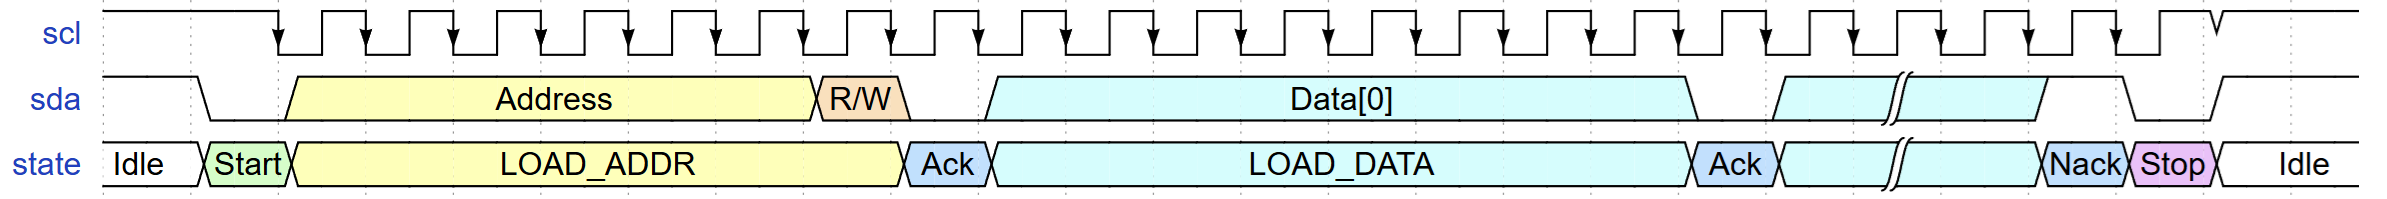
\includegraphics[width=\columnwidth]{./Images/sw_i2c_waveforms.png}
    \vskip 1em
    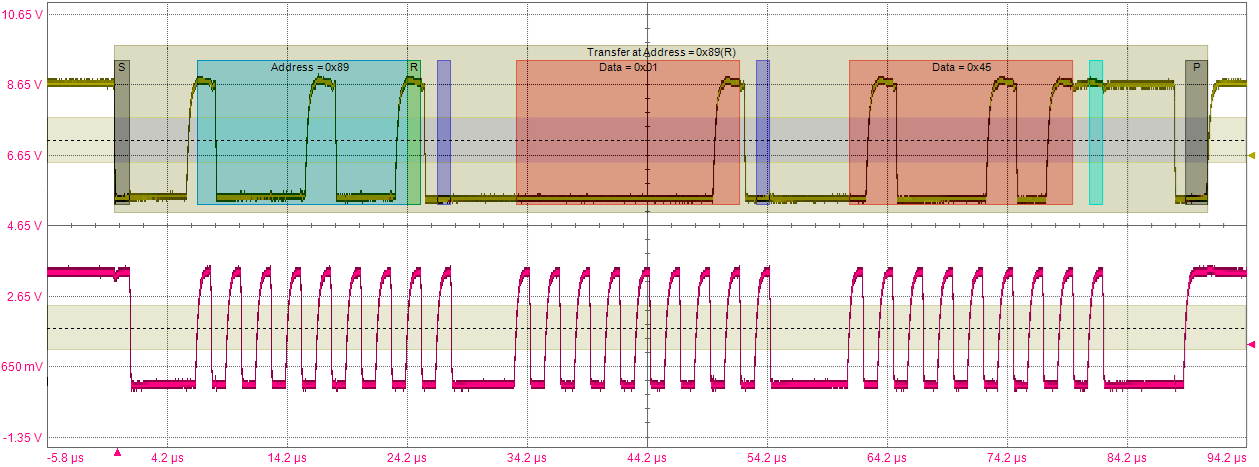
\includegraphics[width=\columnwidth]{./Images/sw_i2c_waveforms_real.png}
    \caption{Formele de undă ce exemplifică funcționarea modulului I2C.}%
\label{fig:sw_i2c_waveforms}
\end{figure}

Acest modul a fost testat cu succes în comunicații bidirecționale, atât cu senzorii de curent de pe placa \gls{aicors}, cât și cu o memorie \gls{eeprom} aflată pe placa de test Nexys Video. În cazul senzorilor de curent, au fost scrise registrele de configurare și calibrare, iar ulterior au fost citite cele care stochează valorile de tensiune, curent și putere măsurate, fiecare dintre acestea având o lățime de 16 biți. O astfel de tranzacție, capturată cu un osciloscop Teledyne Lecroy, este ilustrată în jumătatea de jos a Figurii~\ref{fig:sw_i2c_waveforms}. Tranzacția respectivă implică citirea registrului de curent de la senzorul cu adresa 0x44, transformată în 0x89 după adăugarea bitului R/$\overline{\mbox{W}}$. Comunicarea a avut loc la o frecvență de 140 kHz, cu 40 kHz peste limita specificată pentru modul standard al interfeței. Se poate observa un timp de ridicare semnificativ al semnalelor (aproximativ 400 ns), care limitează creșterea vitezei de transmisie fără a schimba caracteristici hardware ale magistralei. Cu toate acestea, modulul a funcționat stabil și fără erori până la 1 MHz, frecvență la care timpul de ridicare a semnalului a depășit semi-perioada ceasului.

Interfața modulului include, pe lângă câte trei semnale de acces al  \gls{fifo}-urilor (semnal de date, semnal de validare și un semnal de status \gls{fifo}: plin pentru transmitere și gol pentru recepție), și alte semnale și parametrii de interes. Semnalele de control, start și busy, au roluri intuitive, iar adresa este transmisă separat de bitul R/$\overline{\mbox{W}}$, pentru a simplifica logica de control. Un semnal suplimentar indică numărul de octeți dintr-o tranzacție. Parametrii configurabili ai modulului includ: dimensiunea adresei (7 sau 10 biți), dimensiunea \gls{fifo}-urilor și frecvențele ceasurilor de intrare și de transmisie. Acești ultimi parametri sunt folosiți pentru configurarea divizorului de ceas integrat, responsabil cu generarea frecvenței mai reduse necesare logicii de transmisie și recepție. Comunicarea între cele două domenii de ceas, cel rapid al sistemului (de până la 100  MHz) și cel lent al magistralei (până la 1 MHz), este gestionată prin intermediul blocurilor \gls{fifo}, care asigură decuplarea corectă a celor două frecvențe.

\subsection{Serial Peripheral Interface (SPI)}%
\label{spi}
Interfața \gls{spi} este similară cu interfața \gls{i2c} din multe puncte de vedere, ambele fiind utilizate pentru comunicații seriale pe distanțe scurte între dispozitive master și slave. Totuși, diferențele principale dintre ele oferă interfeței \gls{spi} o eficiență și performanță superioare. Spre deosebire de magistrala \gls{i2c}, care folosește două fire, \gls{spi} utilizează cel puțin patru: două pentru transmiterea datelor în ambele direcții (uneori pot fi combinate într-un singur semnal, reducând protocolul la half-duplex), un fir pentru semnalul de ceas și câte un fir individual pentru selecția fiecărui dispozitiv slave. Astfel, se elimină necesitatea alocării de adrese dispozitivelor și permite transferul simultan de date bidirecțional. În plus, interfața utilizează semnale de tip push-pull, spre deosebire de open-drain din \gls{i2c}, permițând viteze de transfer mai mari, cu frecvențe de până la 50 MHz. Această interfață este utilizată pentru comunicația dintre placa \gls{aicors} și modulul \gls{obc} al nanosatelitului, printr-o variantă diferențială, \gls{lvds} \gls{spi}, care asigură o rezistență sporită la zgomot.

Spre deosebire de modulul \gls{i2c}, dezvoltat ca fiind master, modulul \gls{spi} din \gls{fpga}-ul \gls{aicors} este implementat ca slave, fiind semnificativ mai simplu și activat doar la comanda \gls{obc}-ului. Diagrama funcțională a acestui modul este prezentată în Figura~\ref{fig:sw_spi_general_diagram}. Semnalul de start al modulului este transmis de către \gls{obc} prin firul \gls{cs}, iar datele sunt transferate prin semnalul \gls{miso} și printr-un buffer OBUFDS, semnalul \gls{mosi} nefiind utilizat, deoarece modulul este destinat doar pentru transmitere (acesta este totuși utilizat pentru a scrie date în memoria flash a plăcii). Semnalele \gls{cs} și \gls{sck} trec prin buffere IBUFDS, care le convertesc din semnale diferențiale în semnale single-ended, iar apoi printr-o serie de \gls{ff}-uri, inserate toate într-un bloc de comparație pentru a implementa un detector de front. Această metodă bazată pe registre de deplasare este folosită pentru a crea un filtru adițional împotriva zgomotului prezent pe magistrală. Detectoarele de front rezultate conduc atât logica internă de încărcare și deplasare a registrului de shiftare care gestionează datele transmise, cât și semnalele de stare, precum semnalul busy.

\begin{figure}[h!]
    \centering
    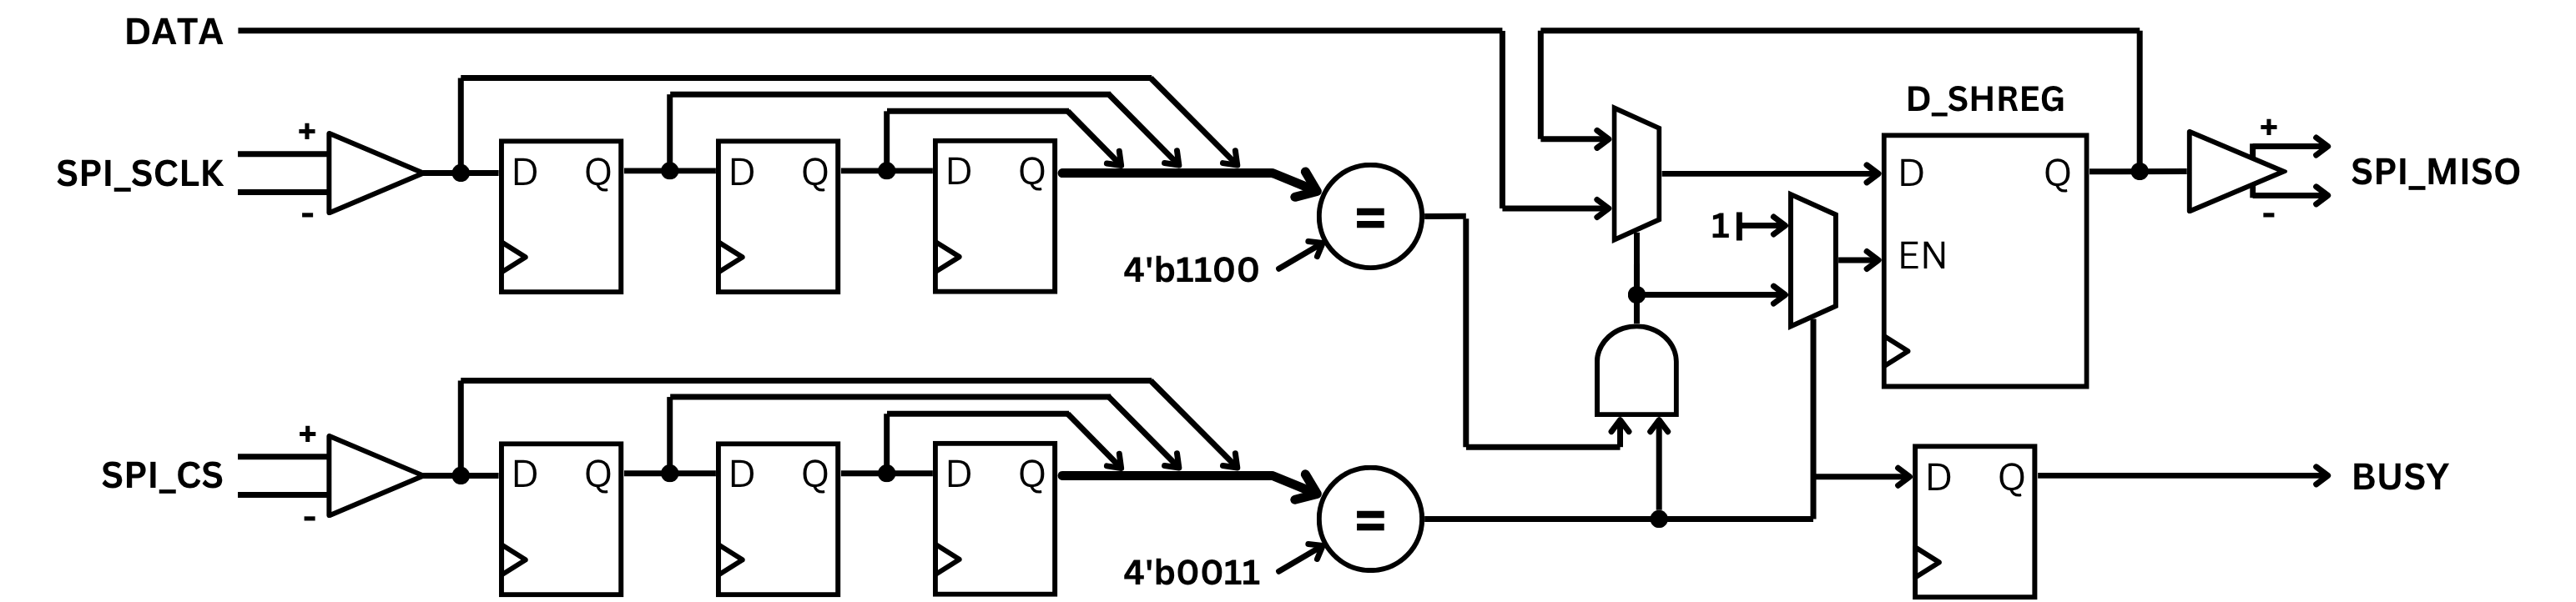
\includegraphics[width=\columnwidth]{./Images/sw_spi_general_diagram.png}
    \caption{Schema bloc a modulului Verilog SPI.}%
\label{fig:sw_spi_general_diagram}
\end{figure}

Acest modul funcționează la frecvențe ale magistralei de cel puțin zece ori mai mici decât frecvența de ceas a sistemului și este configurabil printr-o serie de parametri, precum: dimensiunea filtrelor de zgomot, dimensiunea pachetului de date și ordinea transmiterii sale (MSB-first sau LSB-first), precum și modul de funcționare \gls{spi}. Cele patru moduri standardizate sunt determinate de combinațiile între polaritatea (CPOL) și faza (CPHA) semnalului de ceas, care determină fronturile de eșantionare și transmitere a datelor. Funcționalitatea modulului a fost verificată cu succes, prin transmiterea unor pachete de date de test către un Arduino Due. O astfel de tranzacție este prezentată în Figura~\ref{fig:sw_spi_waveforms_real}, unde, de sus în jos, sunt ilustrate semnalele \gls{cs}, \gls{sck} și \gls{miso}.

\begin{figure}[ht!]
    \centering
    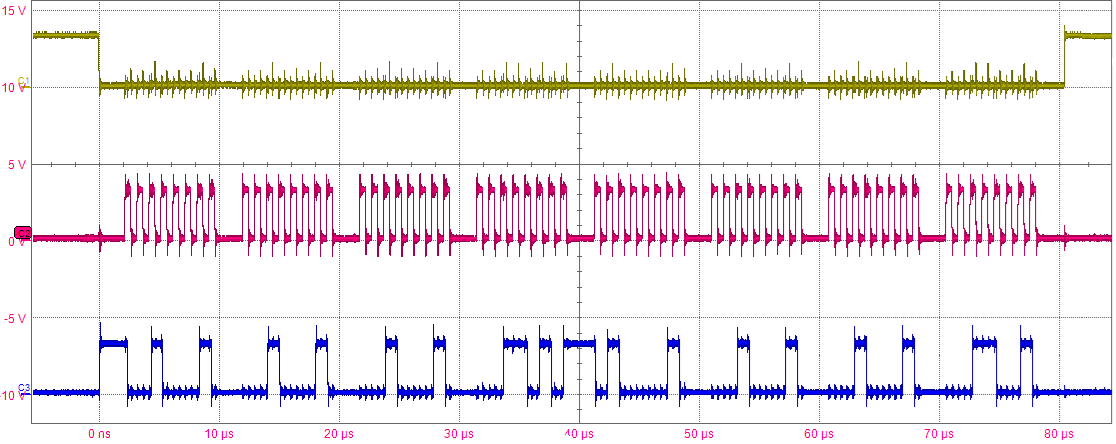
\includegraphics[width=\columnwidth]{./Images/sw_spi_waveforms_real.png}
    \caption{Formele de undă ce exemplifică funcționarea modulului SPI.}%
\label{fig:sw_spi_waveforms_real}
\end{figure}

Structura pachetului de date transmis către \gls{obc} este detaliată în această secțiune. Câmpurile acestui pachet și numărul biților alocați, respectiv numărul de biți activ folosiți de fiecare, sunt prezentate în Tabelul~\ref{tab:sw_spi_packet}. Majoritatea biților neutilizați activ sunt folosiți pentru inserarea de coduri checksum auxiliare, oferind protecție suplimentară pe durata transmisiei. Pachetul este format dintr-o valoare generală, comună tuturor tranzacțiilor, urmată de patru câmpuri specifice fiecărui \gls{seu} stocat în \gls{fifo}-ul modulului \gls{du}.
\begin{itemize}
    \item \textbf{Status}: octet pe 8 biți care conține mai multe semnale de stare esențiale. Acesta permite \gls{obc}-ului să decidă dacă este necesară continuarea citirii întregului pachet, sau dacă se poate opri, astfel salvând puțină energie electrică.
    \begin{itemize}
        \item Bitul 0: indică dacă mai există pachete de date disponibile în \gls{fifo}-ul modulului \gls{du}.
        \item Bitul 1: indică dacă a existat un eveniment de pierdere a alimentării plăcii (brown-out) de la ultima tranzacție \gls{spi}.
        \item Bitul 2: semnalează apariția unui \gls{seu} logic în registrele \gls{tmr} ale programului.
        \item Următorii trei biți sunt alocați semnalelor provenite din modulul \gls{sem}. Bitul 3 indică apariția unei erori necorectabile în memoria de configurare a \gls{fpga}-ului.
        \item Bitul 4--5: valoarea celor mai puțini semnificativi doi biți ai contorului de erori. 
        \item Bitul 6 are valoarea 1 și este rezervat pentru viitoare implementări ale unui model AI.
        \item Bitul 7: un bit de paritate pentru validarea corectitudinii registrului. Dacă nu există mai multe erori decât cele stocate în registrul status și nu există alte pachete de transmis, tranzacția poate fi întreruptă după acest octet. 
    \end{itemize}
    \item \textbf{Scan number}: contor pe 16 biți care înregistrează numărul de scanări ale memoriilor, efectuate până la detectarea unui \gls{seu}. Astfel, cunoscându-se frecvența și durata unei scanări, acest câmp permite determinarea momentului la care a avut loc eroarea.
    \item \textbf{SEU index}: valoare pe 9 biți care identifică memoria \gls{bram} sau \gls{lutram} în care a apărut evenimentul \gls{seu}. Sunt prezente 356 de \gls{bram}-uri și 40 de \gls{lutram}-uri, codificate consecutiv. În total 405, valoare sub \(2^9 - 1\). Cei 7 biți rămași din alocarea pe 16 biți sunt folosiți pentru adăugarea unui checksum.
    \item \textbf{SEU address}: câmp pe 11 biți, între 0 și 2047, ce reprezintă adresa memoriei la care a apărut evenimentul \gls{seu}. Diferența până la 16 va fi utilizată pentru adăugarea unui cod checksum.
    \item \textbf{SEU data}: valoarea pe 18 biți reprezentând o mască de bit-flip-uri cauzate de evenimentele \gls{seu}. Conține un șir de biți de \enquote{0}, cu biți de \enquote{1} în pozițiile unde au fost identificate erori. Cei 6 biți suplimentari sunt folosiți pentru extinderea contorului de erori din modulul \gls{sem}.
\end{itemize}

\begin{table}[h!]
  \centering
  \renewcommand{\arraystretch}{1.3}
  \caption{Structura unui pachet SPI.}%
  \label{tab:sw_spi_packet}
  \begin{tabular}{C{2.5cm} L{3.3cm} C{3cm} C{3cm} C{3cm}}
    \toprule
    \textbf{Nr.} & \textbf{Nume} & \textbf{Biți alocați} & \textbf{Biți folosiți} & \textbf{Biți liberi}\\
    \midrule
        1 & Status      & 8 & 8 & 0 \\
        2 & Scan number & 16 & 16 & 0 \\
        3 & SEU index   & 16 & 9 & 7 \\
        4 & SEU address & 16 & 11 & 5 \\
        5 & SEU data    & 24 & 24 & 6 \\
    \midrule
        6 & Total       & 80 & 68 & 12 \\
    \bottomrule
  \end{tabular}
\end{table}

Codurile checksum vor fi generate folosind un algoritm de sume pe blocuri cu XOR, fiind posibile mai multe strategii de inserare: fie aplicarea unui singur cod pentru întregul pachet, fie aplicarea de coduri pentru fiecare valoare sau pentru grupuri de două valori, utilizând astfel toți biții nefolosiți. În viitor, acest modul poate fi extins pentru a permite și recepția de comenzi, transformându-l într-un modul \gls{spi} complet. Astfel, se va putea adăuga un cod \gls{crc} pentru fiecare pachet și implementa o metodă de retransmitere a pachetelor corupte.

% ---------------------------------------------------------------

\chapter{Proiectarea și implementarea PCB-ului suport}
Până în acest punct a fost prezentată partea software a proiectului, respectiv circuitul implementat pe \gls{fpga} pentru detecția radiației cosmice și transmiterea valorilor relevante către \gls{obc}-ul nanosatelitului. În secțiunile următoare este descris procesul de proiectare a cablajului imprimat pe care va fi montat atât \gls{fpga}-ul țintă, cât și circuitele și dispozitivele auxiliare necesare funcționării sale. Principalele constrângeri de proiectare sunt: spațiul limitat disponibil, generarea tensiunilor corecte de alimentare, reducerea consumului de energie și asigurarea robusteții și fiabilității în mediul spațial extrem.

Procesul de proiectare a implicat realizarea unei versiuni de test și, ulterior, a unei versiuni finale, în care au fost corectate problemele identificate și aduse îmbunătățiri acolo unde a fost posibil. Prima versiune a inclus și module auxiliare care nu au fost păstrate în versiunea a doua, precum un conector \gls{usb} și un slot pentru card SD, utile pentru testarea și depanarea mai ușoară, precum și pentru explorarea unor alternative de implementare pentru anumite sisteme. Întregul proces de proiectare și dezvoltare al primei versiuni a fost documentat anterior într-un articol realizat cu un coautor, \emph{\enquote{The Design and Implementation of an FPGA-based Cosmic Radiation Sensor PCB}}~\cite{icemes}, din care au fost preluate anumite idei și imagini utilizate și în acest capitol.

O parte dintre circuite și componente au fost inspirate din schemele plăcilor de evaluare AC701 de la AMD și Nexys Video de la Digilent, deoarece ambele utilizează același model de \gls{fpga}, oferind un bun punct de plecare pentru proiectarea structurii de alimentare și configurare. Ambele versiuni ale \gls{pcb}-ului au fost fabricate și asamblate de compania JLCPCB, bazată în China. Au fost produse câte cinci unități pentru fiecare dintre cele două versiuni ale plăcii, dintre care trei au fost asamblate cu componente. Acest serviciu a fost ales în locul unor opțiuni locale precum Eurocircuits, datorită costului redus, performanței ridicate, ușurinței de utilizare a serviciilor acestora și rapidității execuției comenzii. De asemenea, JLCPCB oferă o gama extinsă de opțiuni de fabricare pentru personalizarea fiecărui \gls{pcb}, un depozit propriu de componente disponibile imediat pentru asamblarea \gls{pcb}-ului, precum și posibilitatea de a livra componente suplimentare direct în contul personal pentru utilizarea în procesul de producție.

În continuare sunt prezentate aspectele generale ale proiectării \gls{pcb}-urilor, de la realizarea schemei electrice până la layout-ul fizic. Ulterior, sunt detaliate principalele blocuri funcționale ale plăcii: sistemul de alimentare și generarea celor patru tensiuni necesare, amplasarea \gls{fpga}-ului și a memoriei externe, componentele de depanare și sistemele auxiliare. Capitolul se încheie cu o comparație a celor două versiuni ale \gls{pcb}-ului, punând accent pe diferențele, modificările și îmbunătățirile aduse variantei finale, urmată de o scurtă concluzie ilustrativă în care sunt prezentate cele două plăci.

\section{Constrângeri și cerințe generale}
Dimensiunea și forma generală a plăcii au fost impuse de \acrfull{jaxa} pentru a asigura integritatea perfectă în structura nanosatelitului. În momentul proiectării primei versiuni ale \gls{pcb}-ului, specificațiile geometrice și alte aspecte nu erau încă definite, astfel că prima versiune a plăcii a fost realizată cu dimensiunile de 96 $\times$ 90 mm și o formă dreptunghiulară cu colțuri rotunjite. Ulterior, odată cu primirea desenului tehnic oficial, dimensiunea a fost redusă la 86 $\times$ 90 mm, rezultând o suprafața efectivă de plasare a componentelor de aproximativ 73 cm\textsuperscript{2}, după excluderea zonelor rezervate pentru găurile de montare și conectorul principal.

Desenul tehnic utilizat pentru proiectarea versiunii finale a plăcii este ilustrat în Figura~\ref{fig:hw_pcb_cad_drawing}, unde se pot observa forma colțurilor, amplasarea găurilor de montare și a conectorului principal, precum și mai multe zone hașurate. Aceste zone marchează constrângeri specifice privind plasarea și înălțimea componentelor. Zona superioară interzice amplasarea oricărei componente pe ambele fețe ale \gls{pcb}-ului, iar zonele laterale restricționează montarea de componente cu înălțimi mai mari de 1.5 mm pe partea superioară a plăcii și 2 mm pe fața inferioară. Pentru a evita orice risc de interferență mecanică sau electrică, s-a decis excluderea completă a componentelor în aceste regiuni. Astfel, suprafața totală a fost redusă la aproximativ 55 cm\textsuperscript{2} pe fiecare parte a \gls{pcb}-ului.

Găurile de montare au un diametru de 3.8 mm, extinzându-se până la 5.8 mm prin includerea unei zone expuse de cupru pentru conectarea masei la structura metalică a satelitului. Toți conectorii utilizați sunt de tip header, având pini de 1 mm și pasul (pitch) de 2.54 mm.

\begin{figure}[ht!]
    \centering
    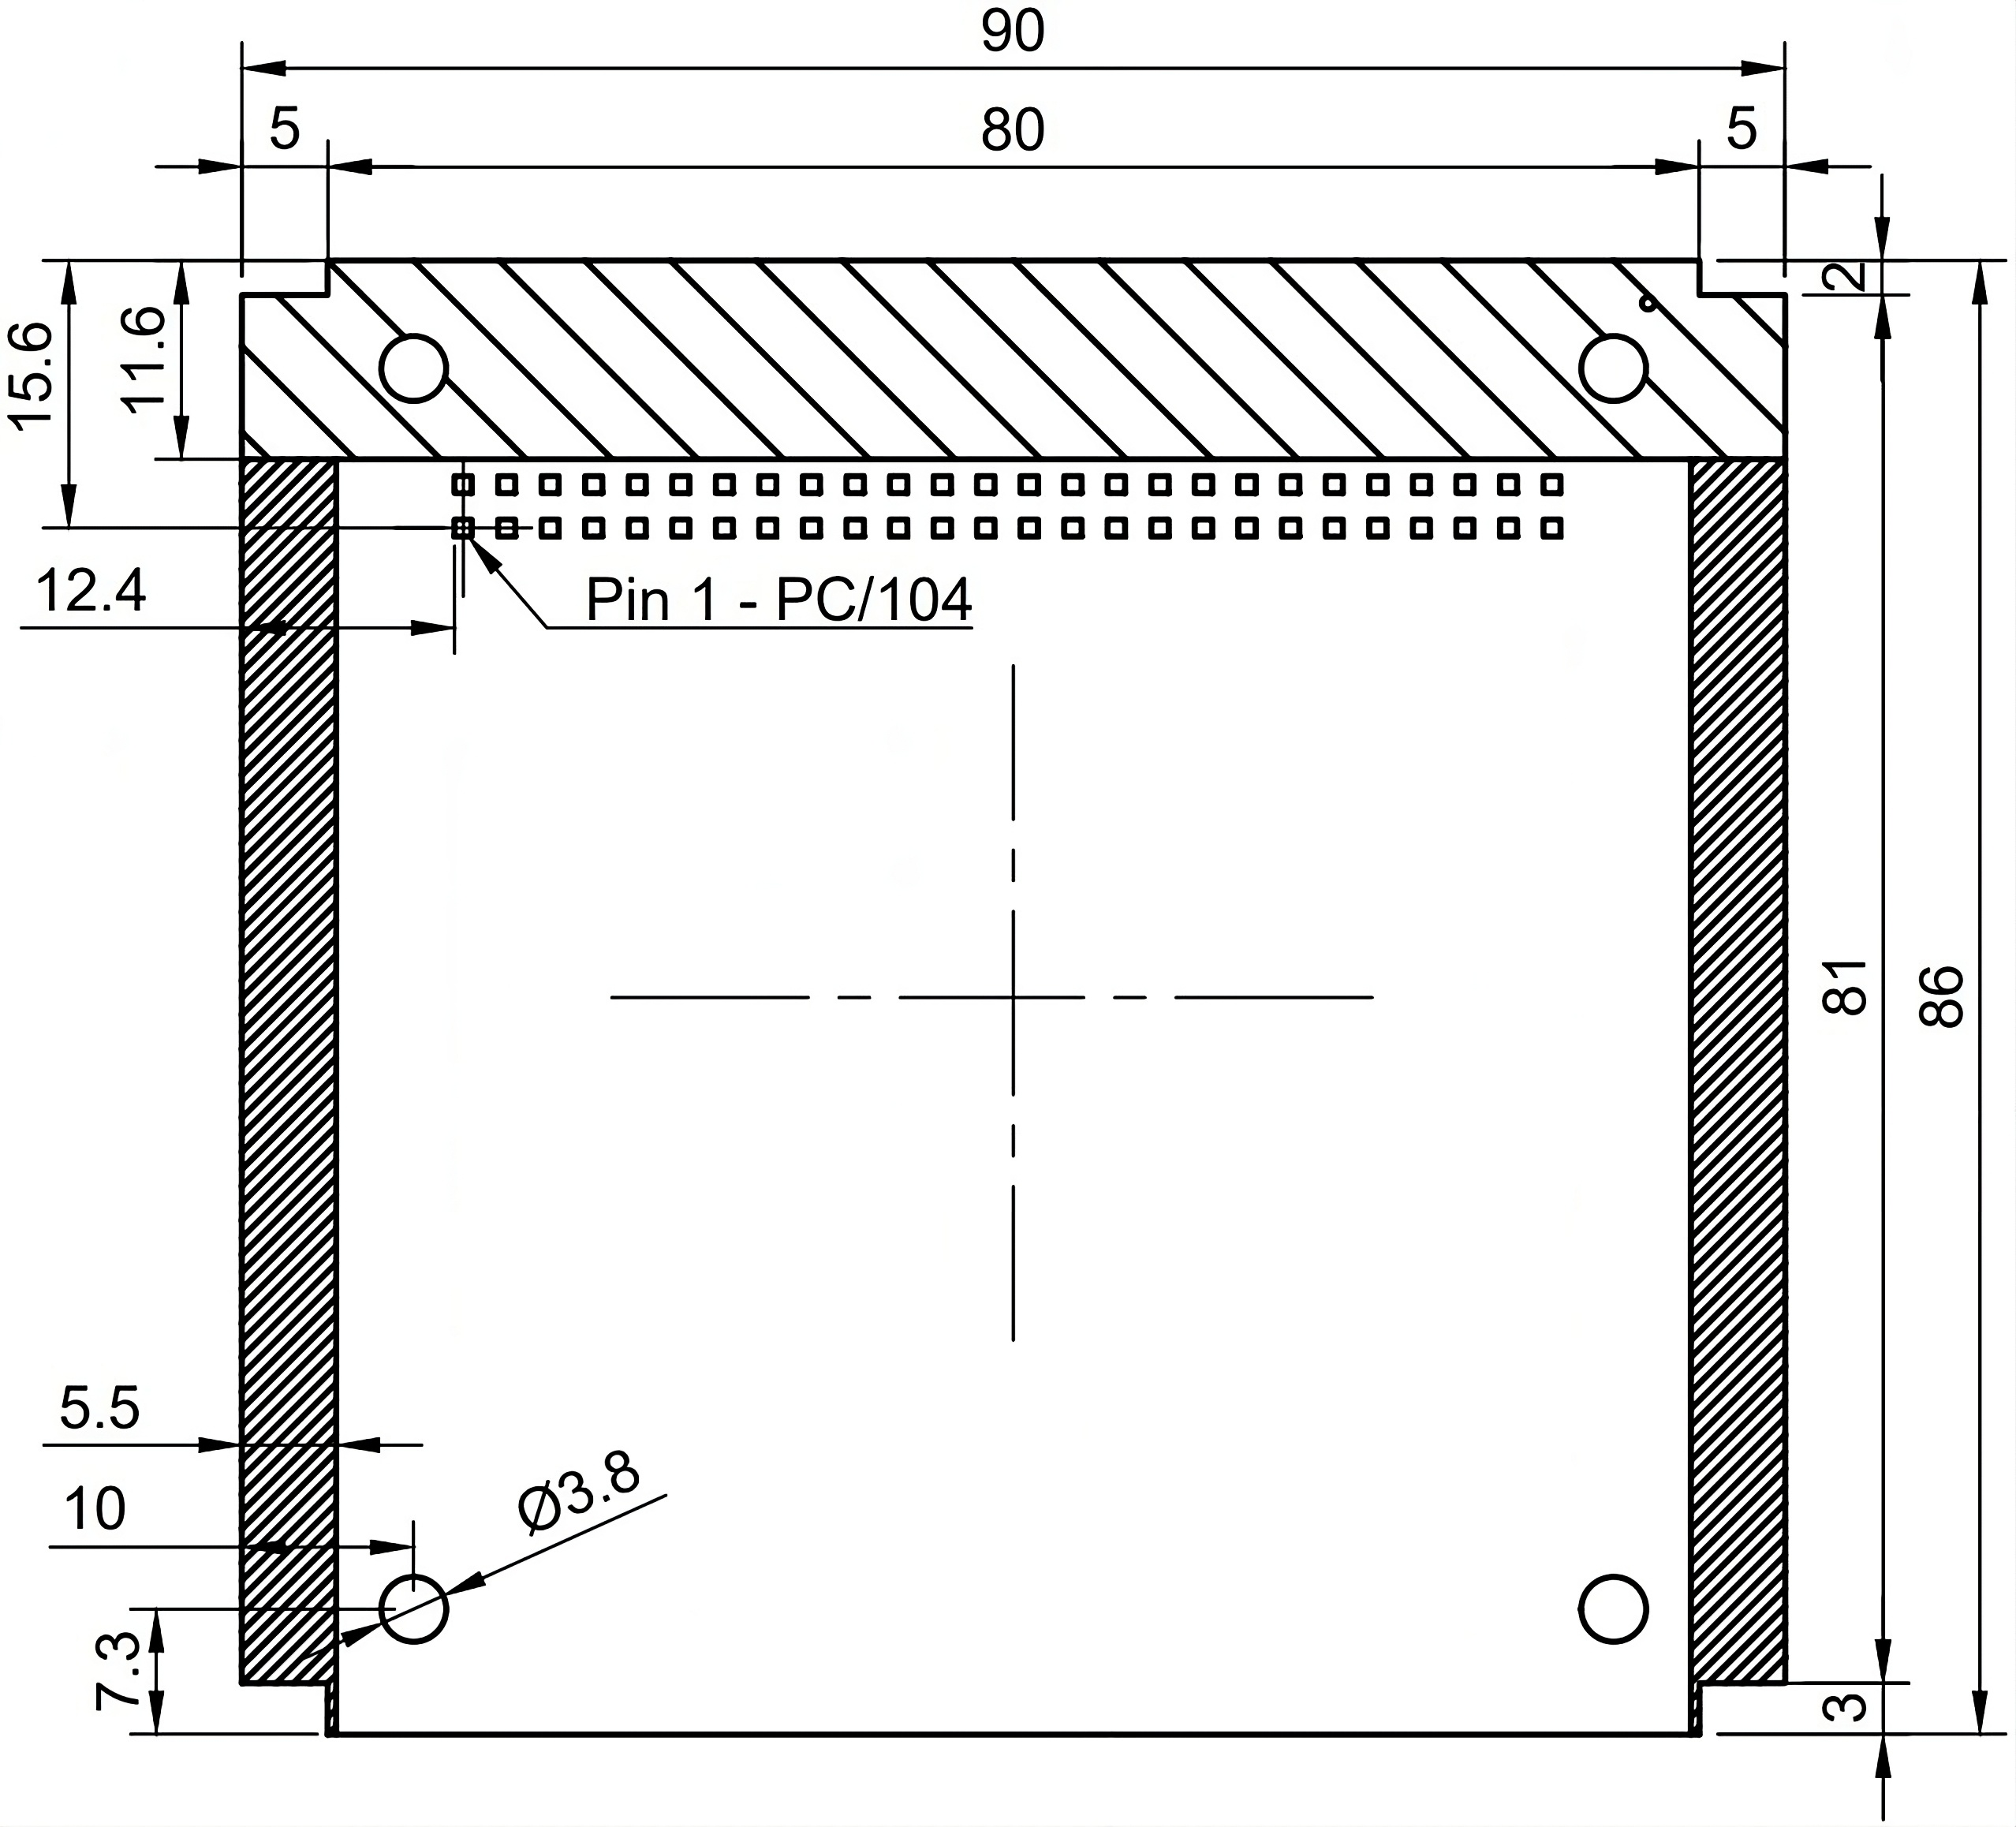
\includegraphics[width=0.7\columnwidth]{./Images/hw_pcb_cad_drawing.png}
    \caption{Schema tehnică a versiunii finale a PCB-ului AICoRS.}%
    \label{fig:hw_pcb_cad_drawing}
\end{figure}

În ceea ce privește structura internă a \gls{pcb}-ului, a fost ales un stack-up cu șase straturi metalizate pentru prima versiune a plăcii și o grosime totală de 1.6 mm, oferind un spațiu suficient pentru rutarea completă a semnalelor și pentru implementarea planurilor de masă și alimentare. Configurația exactă este prezentată în Tabelul~\ref{tab:hw_pcb_v1_layers}, care include grosimea, tipul de material, permitivitatea relativă și distribuția funcțională a fiecărui strat: două straturi exterioare dedicate rutării semnalelor, două planuri de masă și două planuri de alimentare.

\begin{table}[h!]
    \footnotesize
    \centering
    \renewcommand{\arraystretch}{1.5} 
    \caption{Stackup-ul primei versiuni a PCB-ului.}%
    \label{tab:hw_pcb_v1_layers}
    \begin{tabular}{C{1.2cm} L{2cm} C{3.2cm} L{3.5cm} L{2.5cm} C{2cm}}
		\toprule
			\textbf{Nr.} & 
            \textbf{Nume} & 
            \textbf{Grosime [mm]} & 
            \textbf{Rol} & 
            \textbf{Material} & 
            \textbf{Permitivitate relativă}\\
		\midrule
		    1 & Top           & 0.035 & Semnal                & Cupru     & ---  \\
		    2 & Dielectric 1  & 0.203 & PrePreg               & FR4 7628  & 4.4  \\
		    3 & Interior 1    & 0.03  & Plan de masă          & Cupru     & ---  \\
		    4 & Dielectric 2  & 0.25  & Nucleu                & FR4       & 4.6  \\
		    5 & Interior 2    & 0.03  & Plan de alimentare    & Cupru     & ---  \\
		    6 & Dielectric 3  & 0.513  & PrePreg              & FR4 7628  & 4.4  \\
		    7 & Interior 3    & 0.03  & Plan de alimentare    & Cupru     & ---  \\
		    8 & Dielectric 4  & 0.25  & Nucleu                & FR4       & 4.6  \\
		    9 & Interior 4    & 0.03  & Plan de masă          & Cupru     & ---  \\
		    10 & Dielectric 5 & 0.203 & PrePreg               & FR4 7628  & 4.4  \\
		    11 & Bottom       & 0.035 & Semnal                & Cupru     & ---  \\
		\bottomrule
    \end{tabular}
\end{table}

Straturile exterioare (Top și Bottom) au fost alese pentru rutarea semnalelor, facilitând procesul de testare și depanare a fiecărui traseu, precum și obținerea unui control mai precis al impedanței pentru semnalele sensibile. Mediul dielectric dintre trasee și planurile interioare, format parțial din FR4 și parțial din aer, permite o ajustare mai flexibilă a impedanței caracteristice decât în cazul straturilor interioare, unde acesta depinde strict de grosimea și toleranțele materialului dielectric. Sub aceste straturi se află două planuri de masă (Interior 1 și 4). Această configurație contribuie la reducerea căderilor de tensiune pentru curenții de întoarcere, introduce o barieră eficientă împotriva zgomotului între straturile de alimentare și cele de semnal, și simplifică rutarea semnalelor de pe celelalte straturi.

Ultimele două straturi interioare (Interior 2 și 3) sunt dedicate distribuției celor patru tensiuni de alimentare generate de regulatoarele de pe placă, către \gls{fpga} și către celelalte dispozitive de tip \gls{ic}. Primul dintre aceste straturi este utilizat ca un plan uniform pentru 3.3 V, deoarece această tensiune este folosită de majoritatea dispozitivelor de pe placă, în timp ce al doilea strat este rezervat rutării celorlalte trei tensiuni de alimentare. Planurile extinse de cupru și traseele late sunt esențiale pentru a minimiza rezistența de linie și, implicit, pierderile de putere, aspect crucial pentru liniile de alimentare care transportă curenți semnificativi.

Figura~\ref{fig:hw_pcb_v1_diagram} prezintă schema bloc a primei versiuni a plăcuței \gls{aicors}, care include toate circuitele principale: generatoarele de tensiune, conectorul principal PC/104, \gls{fpga}-ul și blocurile adiacente. Jumătatea din dreapta a schemei este dedicată generării celor patru tensiuni de alimentare, asigurării secvenței corecte de activare a acestor tensiuni și monitorizării consumului de energie. Partea din stânga ilustrează toate interfețele de comunicație dintre \gls{fpga} și conectorul principal, cipul de memorie flash utilizat pentru stocarea fișierelor de configurare, precum și alte componente auxiliare.

Dispunerea generală a componentelor pe \gls{pcb} urmează aceeași logică funcțională, fiind împărțită în două blocuri principale: generatorul de energie și blocul \gls{fpga}. După cum se observă în imagine, zona de generare a energiei este separată cât mai mult de restul circuitelor, pentru a reduce cuplarea zgomotului, provenit de la activitatea de comutare, la restul logicii sensibile. \gls{fpga}-ul a fost plasat central, în apropierea conectorului PC/104, pentru a minimiza lungimea traseelor critice de comunicație între \gls{fpga} și \gls{obc}. În plus, toate oscilatoarele de pe \gls{pcb}, cipurile de memorie și alte componente dependente au fost amplasate cât mai aproape de dispozitivele pe care le deservesc.

\begin{figure}[ht!]
    \centering
    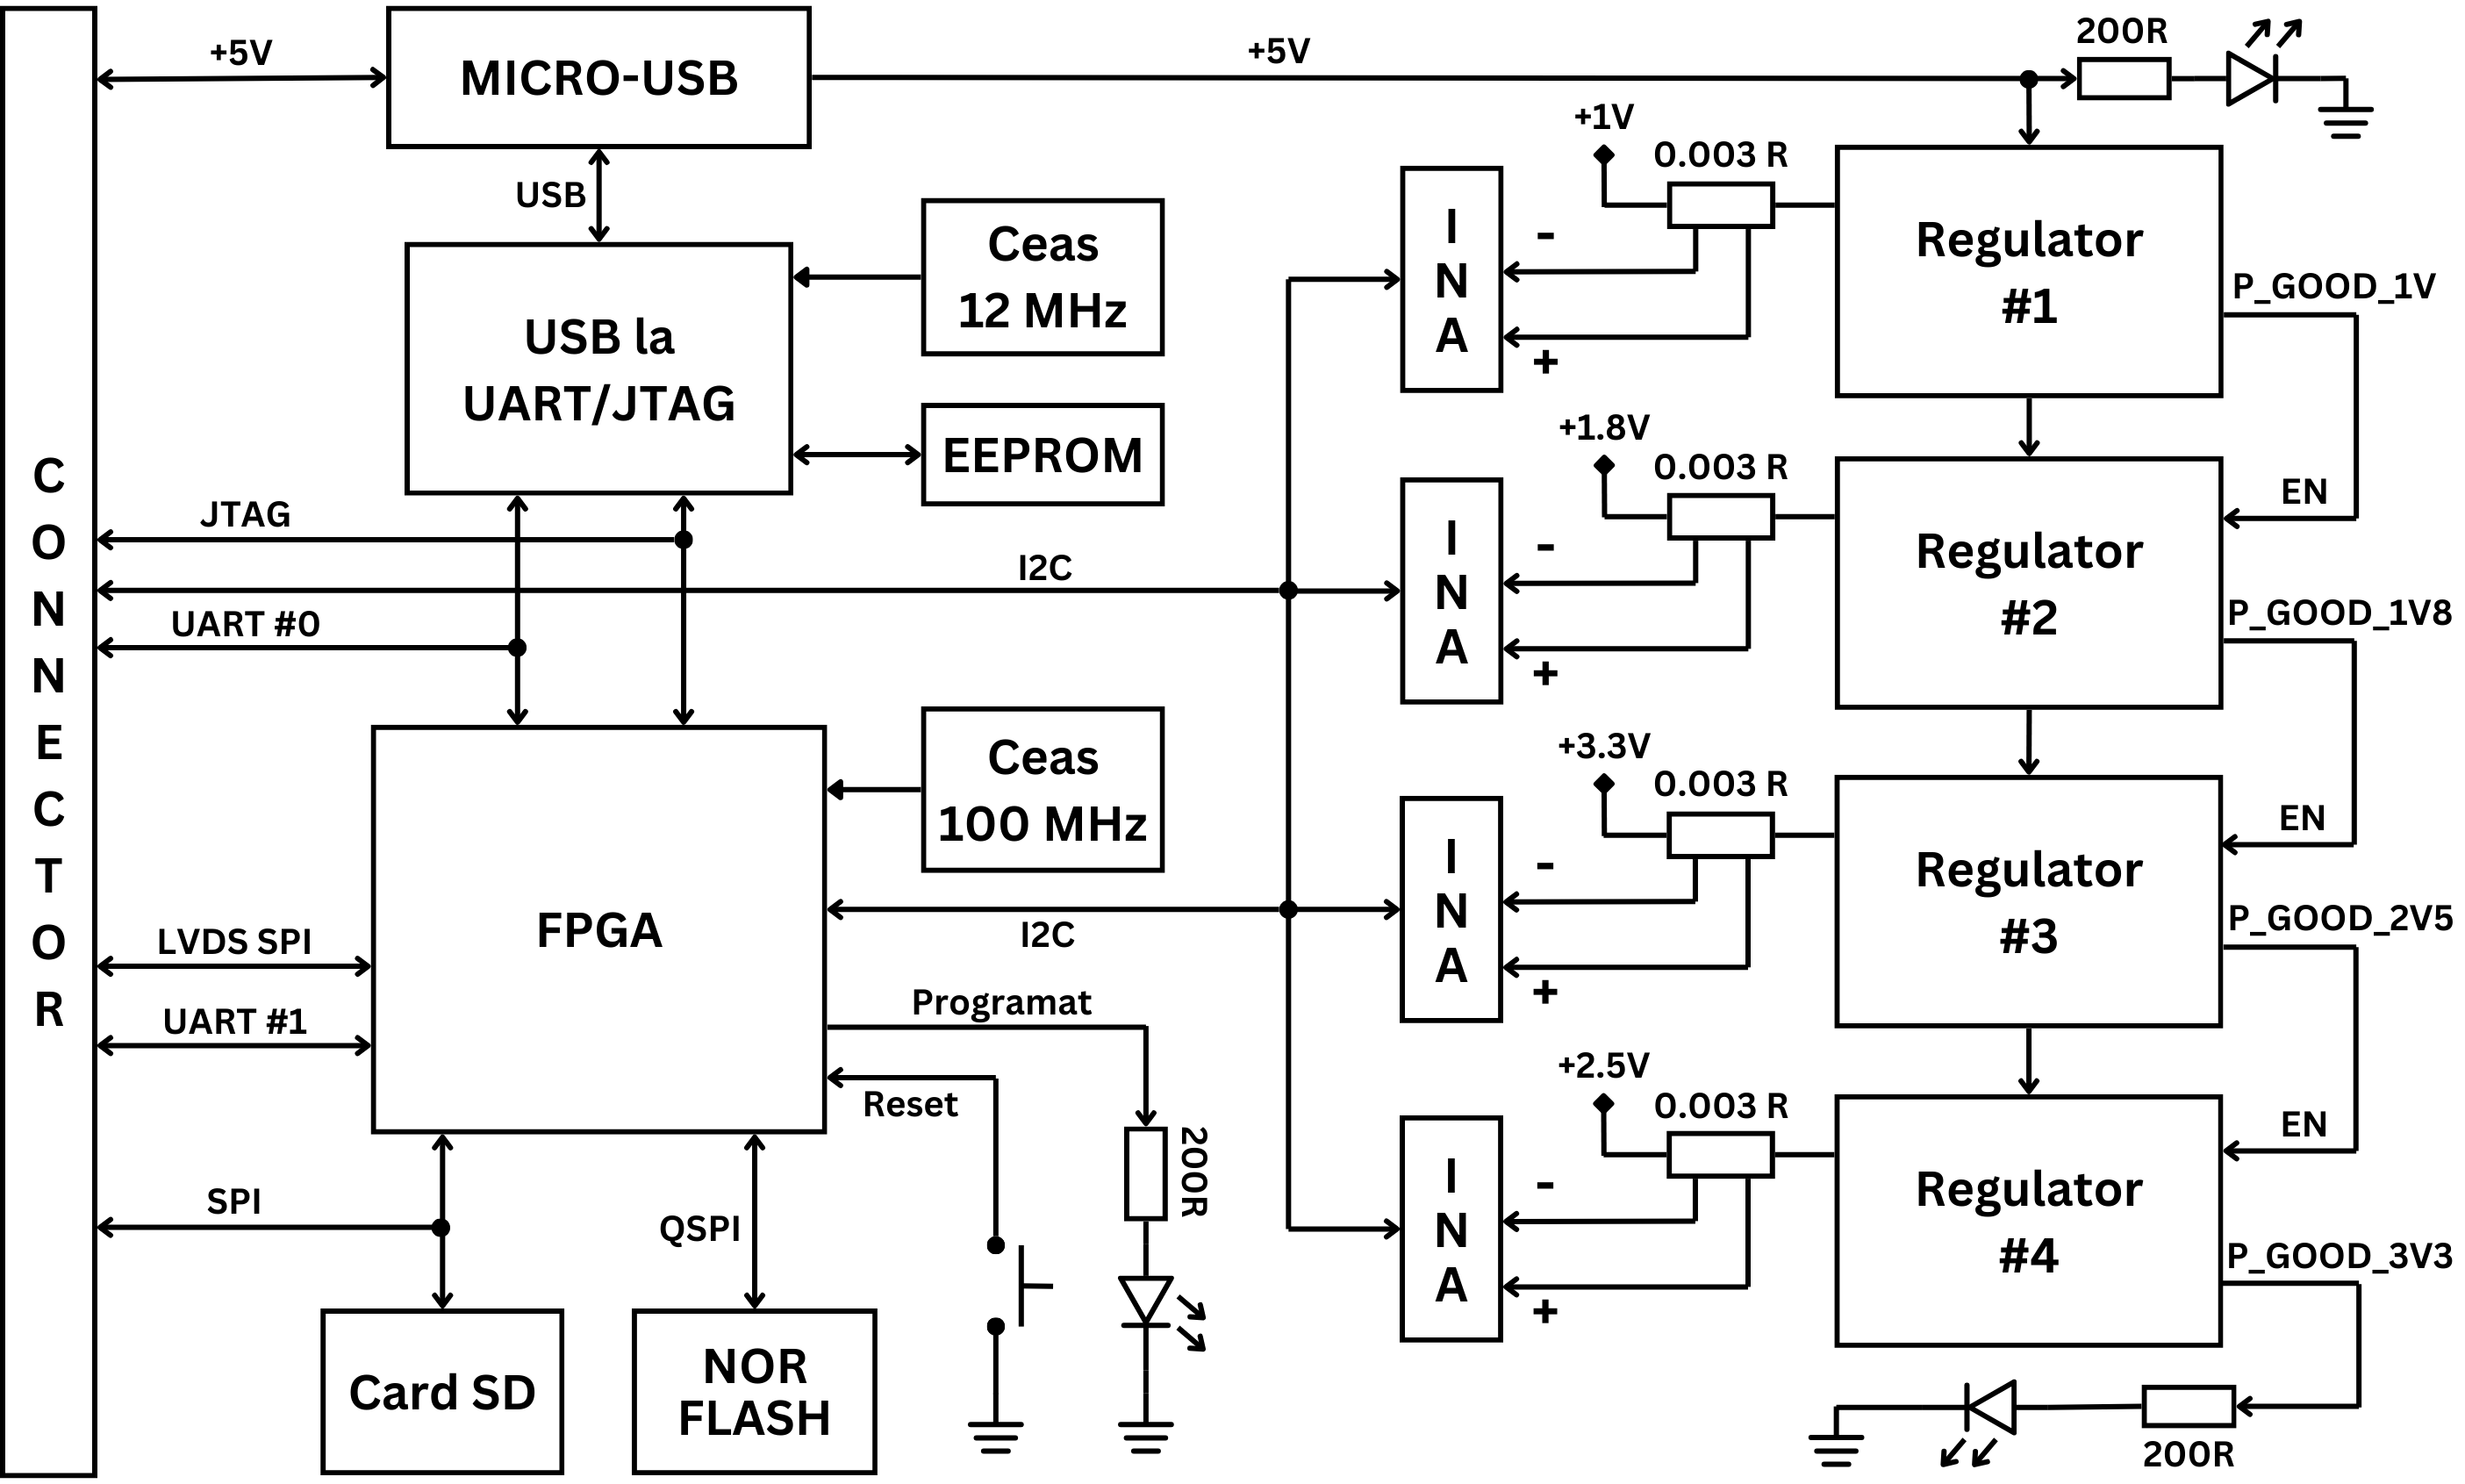
\includegraphics[width=\columnwidth]{./Images/hw_pcb_v1_diagram.png}
    \caption{Schema bloc primei versiuni a PCB-ului AICoRS.}%
\label{fig:hw_pcb_v1_diagram}
\end{figure}

Majoritatea componentelor, împreună cu toate punctele de test și conectorii, au fost plasate pe partea superioară a plăcii, pentru a ușura depanarea și măsurătorile. Pe fața inferioară au fost montate o parte dintre condensatorii de decuplare ai \gls{fpga}-ului și ai regulatoarelor de tensiune, precum și toate jumper-ele, utilizate pentru activarea anumitor circuite sau pentru configurarea conexiunilor interne. 

Toate semnalele au fost rutate cu atenție, respectând principiile de bună practică în proiectarea de circuite, pentru a minimiza zgomotul electric și pentru a asigura fiabilitatea plăcii. Lățimea traseelor a fost aleasă în funcție de rolul acestora: 0.2 mm pentru traseele care conduc semnale și 0.5 mm pentru liniile de alimentare, valorile mai mari reducând căderile de tensiune cauzate de rezistența conductorului. O excepție o reprezintă semnalele care ies direct din \gls{fpga}, care au fost rutate cu o lățime de 0.15 mm până la ieșirea din pachetul \gls{bga}. Majoritatea traseelor au fost plasate în configurație microstrip, însemnând plasarea acestora pe straturile superioare ale \gls{pcb}-ului și nu pe straturile interioare (stripline), pentru a facilita testarea și depanarea, dar și pentru a avea un control mai precis asupra impedanței. În cazul stripline, impedanța este mai greu de controlat datorită straturilor dielectrice de grosime fixă, necesitând trasee mai late, față de cazul microstrip, unde stratul exterior oferă mai multă flexibilitate.

Interfețele care impun o impedanță caracteristică bine definită, precum \gls{lvds} \gls{spi} și \gls{usb}, au fost calibrate cu atenție din punct de vedere al lățimii și al spațierii perechilor diferențiale, pentru a respecta cerințele necesare și pentru a reduce reflexiile de semnal apărute la întâlnirea unei diferențe de impedanță. Unealta folosită pentru a calcula valorile corecte privind dimensiunea traseelor, dar și pentru a evalua alte aspecte referitoare la \gls{pcb}, este Saturn PCB Toolkit. În plus, toate liniile de semnal au fost egalizate ca lungime, atât între semnalele dintr-o pereche diferențială, cât și între semnalele din aceeași interfață. Acest aspect este esențial pentru a preveni decalajele de propagare între semnale, care pot afecta recepția corectă a pachetelor de date și pot compromite integritatea datelor recepționate.

Trecerea semnalelor de pe un strat pe altul s-a realizat prin intermediul vias-urilor. Acestea nu pot fi ignorate deoarece dețin anumite caracteristici electrice care pot afecta integritatea semnalelor. Vias-urile sunt caracterizate de diametrul găurii care trece prin \gls{pcb} și diametrul inelului anular din jurul găurii. Aceste dimensiuni au fost alese în funcție de scopul traseului: 0.3 - 0.6 mm pentru semnale, 0.5 - 0.8 mm pentru vias-urile de alimentare (dimensiunile sunt mai mari din aceleași motive explicate mai sus) și 0.2 - 0.35 mm pentru liniile rutate sub pachetul \gls{bga} al \gls{fpga}-ului. Dimensiunile reduse din zona \gls{fpga}-ului respectă distanțarea minimă de 0.1 mm între pad-urile \gls{bga} și liniile de semnal. Pentru semnalele sensibile care traversează între straturi, precum semnalele diferențiale, au fost adăugate vias-uri de masă în jurul celor de semnal, asigurând o cale de întoarcere a curentului cât mai scurtă și directă. În rețeaua de alimentare, s-au folosit numeroase vias-uri pentru masă și pentru liniile de tensiune, pentru a facilita transferul termic și pentru a asigura o capacitate de transfer al curentului suficient de mare, astfel încât să depășească capacitatea de generare a regulatoarelor de tensiune.

În final, au fost adăugate teardrops pentru a întări zona de tranziție între trasee, pad-uri și vias-uri. Aceste extensii de cupru sunt plasate la intersecția dintre zonele menționate și ajută la robustețea mecanică a conexiunilor și reduc riscul defectelor de fabricație, contribuind la fiabilitatea pe termen lung a plăcii.

\section{Sisteme principale}
\subsection{Regulatoarele de tensiune}
Printre cele mai importante componente ale plăcii \gls{aicors} se numără regulatoarele de tensiune, responsabile de generarea celor patru tensiuni de alimentare necesare sistemului. Acestea sunt implementate cu patru regulatoare în comutație identice, de tipul TPS84320RUQR~\cite{tps84320_datasheet}, ale căror tensiuni de ieșire sunt alese prin modificarea valorilor a doi rezistori conectați la pinii 43 și 35, care formează un divizor de tensiune intern. Aceste regulatoare au fost alese datorită eficienței ridicate de până la 95\%, disipării termice eficiente, funcționarii stabile până la 85 $^{\circ}$C și datorită integrării inductorului și componentelor pasive în același pachet, ceea ce simplifică semnificativ proiectarea și plasarea circuitului. Aceste dispozitive sunt ușor configurabile prin plasarea unor rezistori externi și permit legarea în serie a mai multor regulatoare pentru realizarea unei secvențe de pornire controlate. Primul regulator din lanț permite pornirea următorului regulator doar după stabilizarea completă a tensiunii generate, prin intermediul semnalelor \textit{1V\_VOLTAGE\_EN} și \textit{PWR\_GOOD\_1V}, ilustrate în Figura~\ref{fig:hw_schematic_power}.

În Figura~\ref{fig:hw_schematic_power} este prezentată schema electrică simplificată a modulului regulator de 1 V, primul din secvența 1 V - 1.8 V - 2.5 V - 3.3 V. În partea stângă se află circuitul principal împreună cu condensatori de decuplare, siguranță, mărgea de ferită și rezistori de pull-up, iar în partea dreaptă ieșirea regulatorului este conectată printr-un rezistor de tip shunt la un senzor de curent și de tensiune INA219~\cite{ina219_datasheet}, comunicând prin interfață \gls{i2c}. Acest senzor este folosit pentru monitorizarea în timp real a tensiunilor și curenților de pe fiecare linie de alimentare. În colțul din dreapta-jos al schemei se află un LED de stare, controlat de un \gls{mosfet} de tip N (FDV301N), care indică funcționarea corectă a regulatorului.

\begin{figure}[ht!]
    \vspace{6pt}
    \centering
    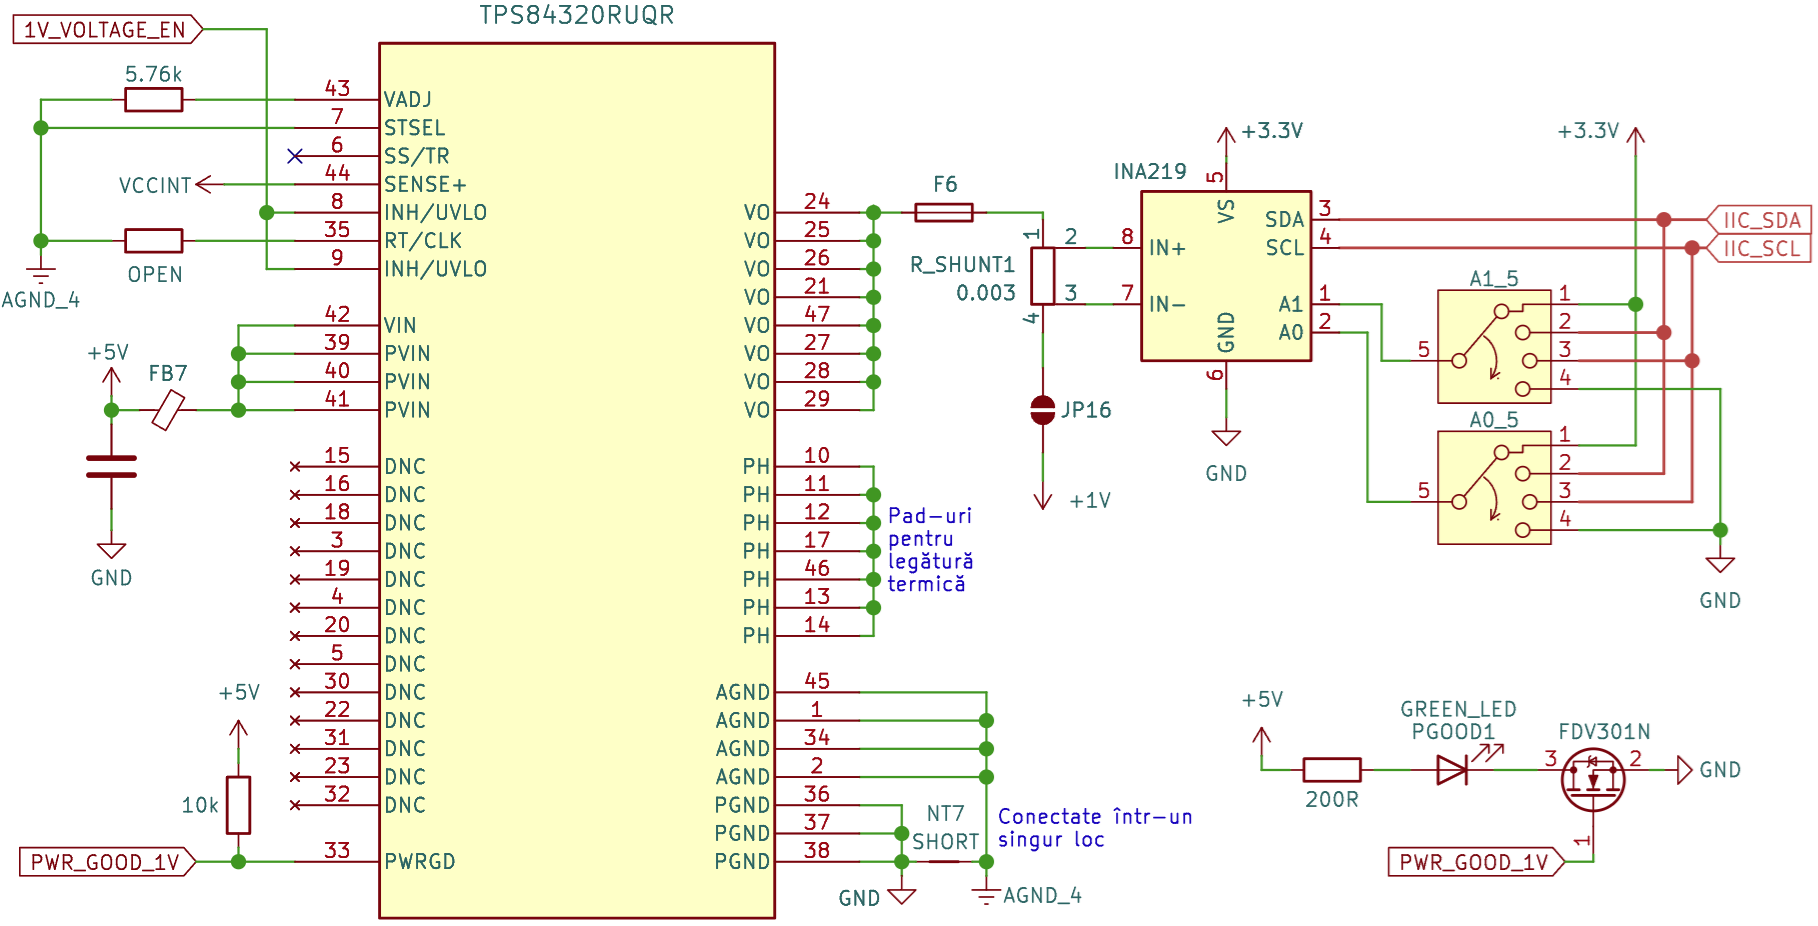
\includegraphics[width=\columnwidth]{./Images/hw_schematic_power.png}
    \caption{Schema electrică simplificată a unui regulator de tensiune.}%
    \label{fig:hw_schematic_power}
    \vspace{6pt}
\end{figure}

Rutarea acestui modul a fost realizată cu atenție, respectând recomandările producătorilor din fișele tehnice ale componentelor. Layout-ul complet al unui regulator de tensiune, împreună cu calea pe care o parcurge curentul, este ilustrat în Figura~\ref{fig:hw_layout_power}. Toate pad-urile care conduc curenți ridicați au fost conectate la zone mari de cupru și multiple vias-uri, pentru a reduce rezistența traseelor și a asigura o capacitate suficientă de transfer al curentului. Zona de masă asociată secțiunilor analogice ale circuitului este localizată sub cip și conectată la planul principal de masă al \gls{pcb}-ului într-un singur punct, pentru a preveni propagarea zgomotului către restul sistemului. Pinul \textit{SENSE+}, utilizat pentru compensarea căderilor de tensiune pe trasee, este rutat separat și este conectat cât mai aproape de pinii de alimentare ai \gls{fpga}-ului, asigurând o reglare precisă a tensiunii. Pentru a putea testa individual fiecare regulator, ieșirea poate fi izolată de restul planului de alimentare printr-un jumper amplasat după rezistorul de shunt.

Cei patru senzori de curent INA219 nu impun cerințe stricte de rutare, fiind dispozitive digitale relativ simple. Conexiunea către rezistorul de shunt este realizată printr-o legătură Kelvin și prin trasee simetrice și de aceeași lungime. Adresele celor patru senzori pot fi configurate prin conectarea pinilor \textit{A1} și \textit{A0} la semnalele: VCC, GND, SDA sau SCL, oferind 16 adrese posibile. Se folosesc doi jumperi cu câte cinci borne pentru configurarea acestor conexiuni. Toți cei patru senzori sunt conectați pe același bus \gls{i2c}, într-o topologie de tip stea, având rolul de slave. Acest tip de conexiune, împreună cu egalizarea lungimilor liniilor SDA și SCL, asigură sincronizarea perfectă a semnalelor și reduce riscul apariției unor erori de transmisie. Acest bus este conectat atât la \gls{fpga}, cât și la conectorul PC/104, permițând astfel controlul și monitorizarea printr-un master extern sau prin \gls{obc}-ul nanosatelitului.

\begin{figure}[ht!]
    \centering
    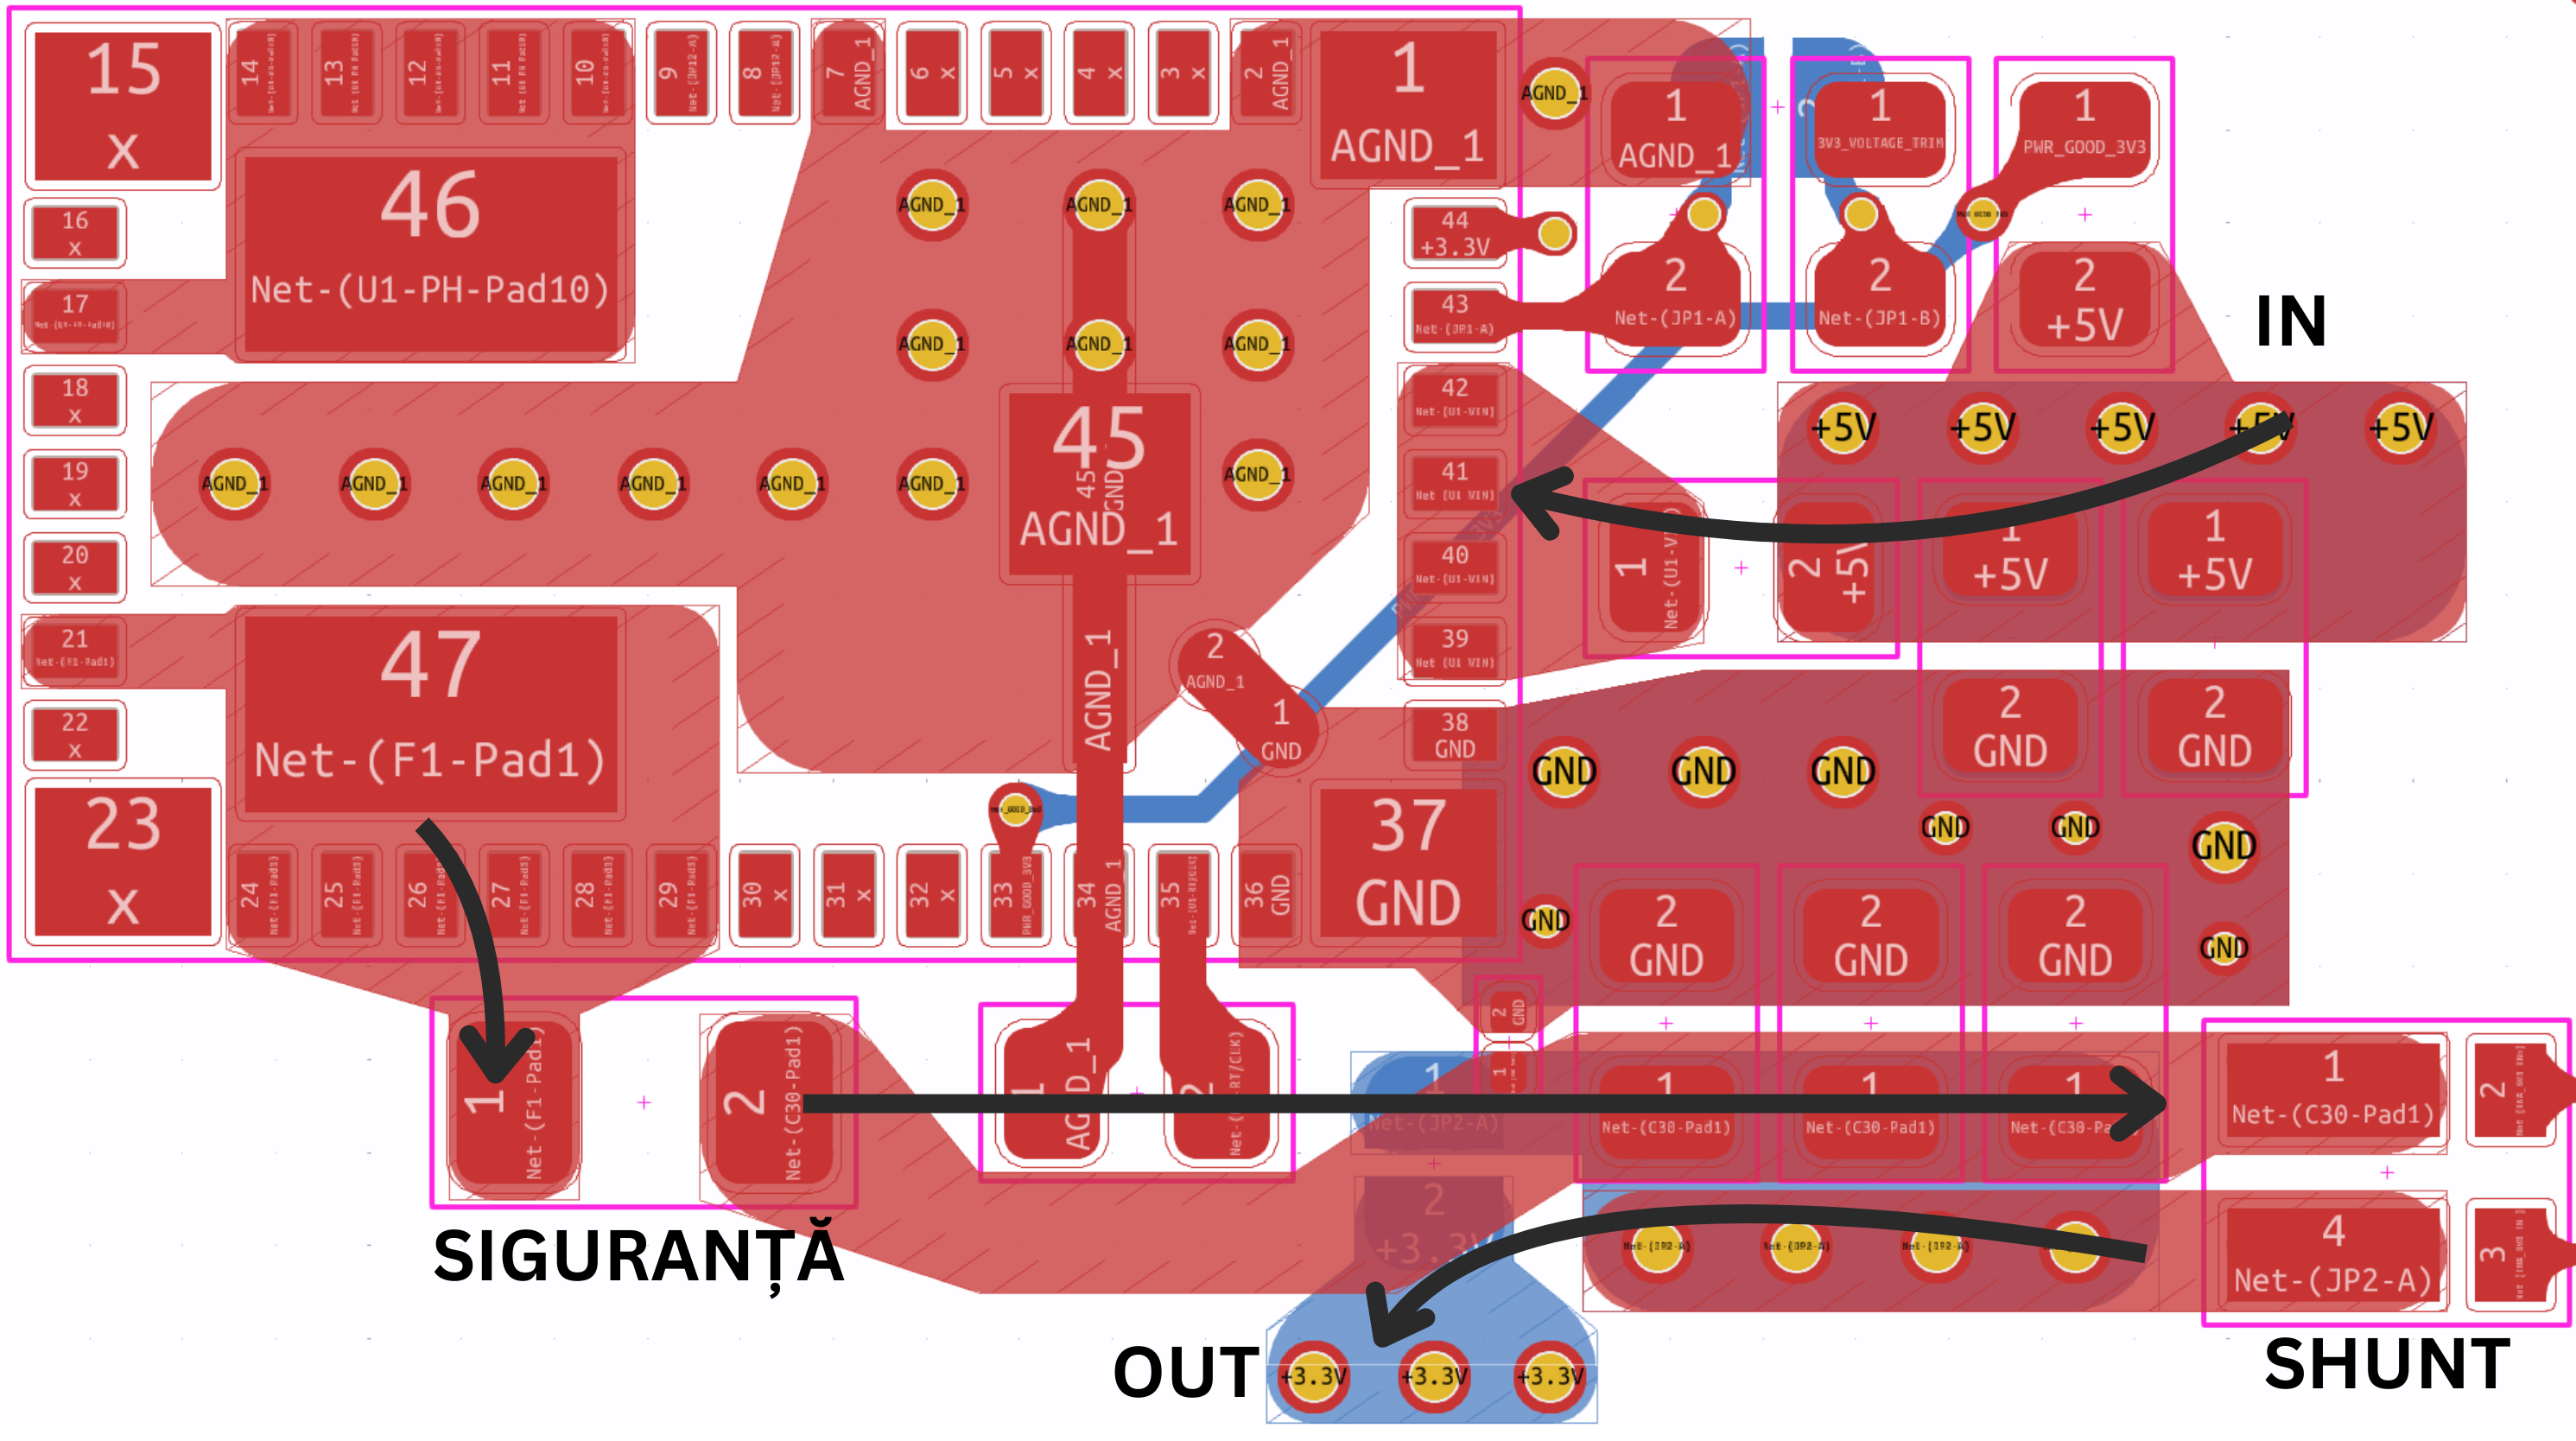
\includegraphics[width=\columnwidth]{./Images/hw_layout_power.png}
    \caption{Traseul curentului prin circuitul regulatorului de tensiune.}%
    \label{fig:hw_layout_power}
\end{figure}

\subsection{Convertorul USB la UART/JTAG}
Pentru a ușura testarea și comunicarea cu dispozitivul \gls{fpga} în prima versiune a plăcii, a fost adăugat un conector Micro-\gls{usb}, permițând conectarea plăcii la un computer prin intermediul unui singur cablu obișnuit. Acesta asigură atât alimentarea plăcii, cât și programarea și comunicarea cu aceasta. Totuși, interfața \gls{usb} este mult prea complexă pentru a fi implementată direct în \gls{fpga} folosind Verilog, necesitând resurse logice care ar putea fi alocate senzorului de radiație. Din acest motiv, s-a optat pentru utilizarea unui cip separat care transformă interfața \gls{usb} în altele mai simple, conectate direct la \gls{fpga}. Cele două interfețe generate sunt \acrfull{uart}, utilizată pentru comunicare asincronă simplă, și \acrfull{jtag}, interfața implicită de configurare și comunicare a dispozitivelor \gls{fpga}.

Cipul ales este FT2232HL~\cite{ft2232h_datasheet} produs de compania FTDI, un convertor \gls{usb} capabil să ofere două interfețe independente. Schema electrică aferentă este prezentată în Figura~\ref{fig:hw_schematic_usb}, unde se pot observa cipul principal, conectorul Micro-\gls{usb}, un oscilator de 12 MHz, necesar funcționării cipului, și un cip de memorie \gls{eeprom} destinat stocării setărilor de configurare ale convertorului.

\begin{figure}[ht!]
    \centering
    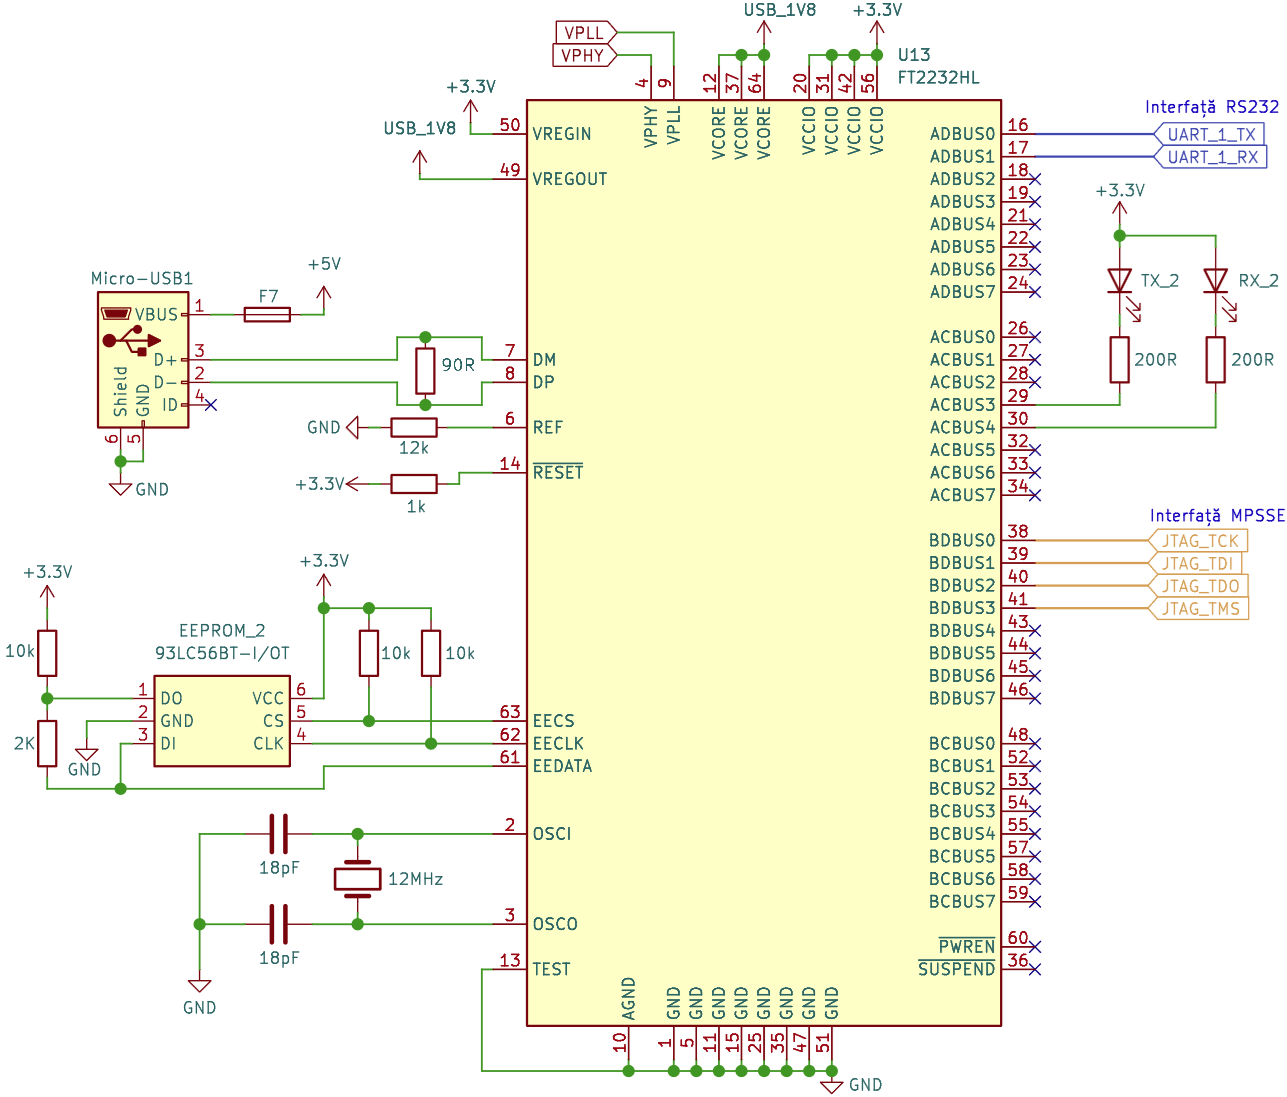
\includegraphics[width=\columnwidth]{./Images/hw_schematic_usb.png}
    \caption{Schema electrică simplificată a convertorului USB la UART/JTAG.}%
    \label{fig:hw_schematic_usb}
\end{figure}

Cipul este alimentat la 3.3 V, necesitând suplimentar și tensiunea de 1.8 V pentru logica internă. Această tensiune poate fi însă generată intern și trebuie legată doar de la pinul de ieșire, printr-un set de condensatori de decuplare la pinii de alimentare. S-a preferat această soluție, în locul conectării la planul general de alimentare, pentru a obține o măsurare mai precisă a curentului consumat de \gls{fpga}, fără influența altor circuite active. Interfața \gls{usb} a fost rutată pe un singur strat, cu trasee cât mai scurte, prin plasarea cipului convertor cât mai aproape de conectorul Micro-\gls{usb}, și a fost terminată cu un rezistor de 90 \(\Omega\), pentru menținerea impedanței caracteristice.

Configurarea cipului se realizează cu aplicația FT\_PROG, pusă la dispoziție de FTDI.\@ Aceasta se instalează pe un computer și permite programarea directă a cipului printr-un cablu \gls{usb}. În aplicație, parametrii de configurare, precum identificatorii de dispozitiv, denumirea portului serial, sursa de alimentare și modurile de funcționare ale celor două porturi, sunt salvați într-un fișier XML. Acest fișier poate fi ulterior scris în memoria \gls{eeprom} atașată cipului. Memoria aleasă este 93LC56BT-I/OT, recomandată de producător, o memorie serială cu capacitatea de 2 Kbit. Deși opțională, lipsa acesteia împiedică configurarea personalizată a cipului, care rămâne astfel în starea implicită, cu prima interfață ca \gls{uart}.

Oscilatorul de 12 MHz a fost amplasat cât mai aproape de cipul convertor, iar sub acesta a fost definită o zonă de interdicție pentru turnarea zonelor de cupru, pentru a minimiza cuplarea zgomotului electric. În procesul de rutare, liniile celor două interfețe au fost reglate pentru a avea aceeași lungime și au fost conectate, de la cipul convertor, la \gls{fpga}, la conectorul PC/104 și la pad-urile de test. Interfața \gls{jtag} a mai fost conectată și la un conector suplimentar de tip header cu șase pini, oferind acces direct la interfața de configurare, în cazul defectării cipului principal. Prin acest conector se poate folosi un cablu programator \gls{jtag}-HS2 de la Digilent, care integrează același tip de cip FTDI.

\subsection{FPGA-ul și circuitele adiacente}
Dispozitivul \gls{fpga} reprezintă componenta cea mai complexă și critică de pe placa \gls{aicors}. A fost ales modelul XC7A200T-2SBG484I din familia Artix-7, cu footprint SBG484, tip Bare-Die Flip-Chip, având dimensiunea de 17\(\times\)17 mm și pitch de 0.8 mm. Acest pachet a fost ales datorită die-ului de siliciu expus, care poate crește sensibilitatea la radiație, dimensiunii compacte, utilă în cazul unui \gls{pcb} compact, și pentru că aplicația dorită nu necesită un număr mare de pini \gls{io}. În schema electrică, \gls{fpga}-ul conține șase bank-uri \gls{io} cu alimentare independentă, un bloc cu transceivere de mare viteză (neutilizat în proiect), un bloc de alimentare generală și un bloc de control și configurare, denumit bank\_0. 

Pentru funcționarea corectă, sunt necesare anumite circuite și cipuri auxiliare: o memorie non-volatilă pentru stocarea fișierelor de configurare, un oscilator de ceas de intrare, comutatoare pentru selecția modurilor de configurare și un număr semnificativ de condensatoare de decuplare. Memoria utilizată este S25FL512S~\cite{flash_datasheet} de la Infineon, iar ceasul este AX3DAF1~\cite{clock_datasheet} de la Abracon, cu frecvența de 100 MHz și interfață \gls{lvds}.

În Figura~\ref{fig:hw_schematic_fpga} este prezentată schema electrică simplificată care include blocul de configurare bank\_0, memoria flash și circuitul de selectare a modului de programare. Blocul 0 conține diverse semnale de status și interfețe de configurare, conectate fie la rezistori de tip pull-up, conform recomandărilor din datasheet, fie la alte dispozitive din sistem. În partea stângă a figurii pot fi observate, de sus în jos: cele patru semnale ale interfeței \gls{jtag}, conectate atât la convertorul \gls{usb}, cât și la conectorul auxiliar, pinul de ceas al interfeței \gls{spi}, utilizată de cipul de memorie flash, trei pini pentru selectarea modului de configurare, trei pini de status și o pereche de pini analogici diferențiali destinați testării unor potențiali senzori de radiație analogici.

Pinii de selecție a modului sunt conectați prin rezistori pull-down la masă, având astfel valoarea 0 implicită, și pot fi setați la valoarea 1 prin intermediul unor jumperi către linia de alimentare. În funcție de combinația acestor trei pini, pot fi selectate opt moduri de configurare, dintre care, în cadrul acestui proiect, au fost utilizate \gls{jtag} (101 --- mod implicit) și Quad-\gls{spi} (100). Pinii \textit{DONE}, \textit{INIT} și \textit{PROGRAM\_B} indică etapele procesului de configurare și pot fi folosiți pentru a verifica dacă \gls{fpga}-ul a fost programat corect. În prima versiune a plăcii, pe lângă rezistorii pull-up, pinul \textit{DONE} a fost conectat la un LED care se aprinde la finalizarea cu succes a configurării, iar pinul \textit{PROGRAM\_B} la un buton către masă, folosit pentru resetarea dispozitivului.

\begin{figure}[ht!]
    \centering
    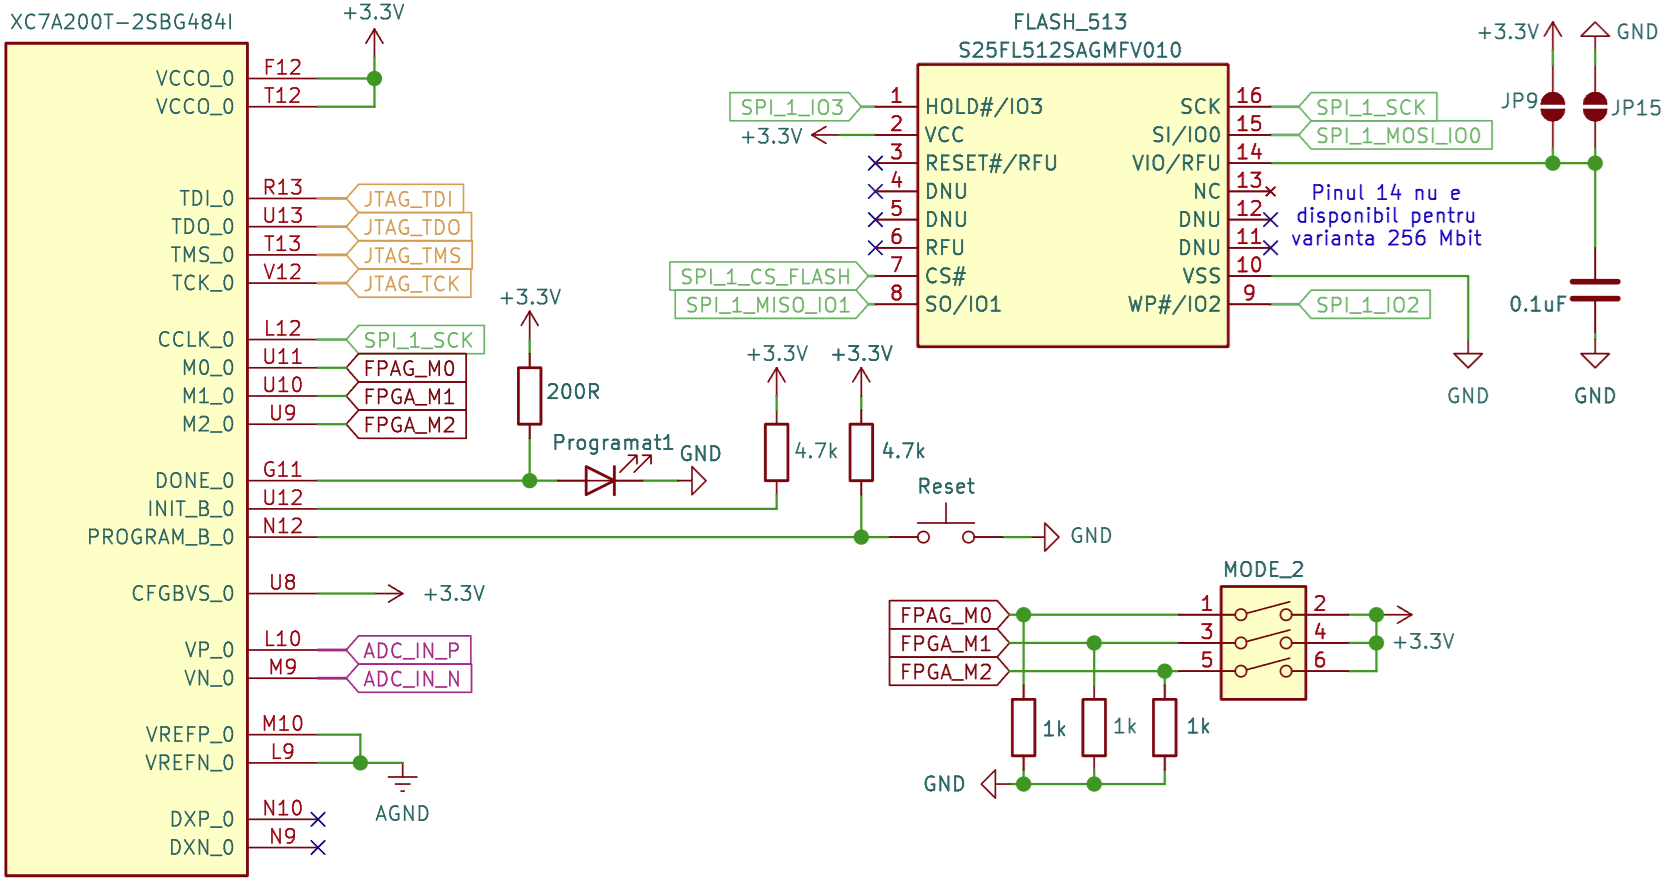
\includegraphics[width=\columnwidth]{./Images/hw_schematic_fpga.png}
    \caption{Schema electrică simplificată a Bank-ului 0 al FPGA-ului și al memoriei flash.}%
    \label{fig:hw_schematic_fpga}
\end{figure}

Memoria flash este ilustrată în colțul din dreapta-sus a figurii. Aceasta este alimentată la 3.3 V pentru a fi compatibilă cu \gls{fpga}-ul, iar toate semnalele interfeței Quad-\gls{spi} sunt conectate la pini dedicați din bank-ul 14, cu excepția pinului de ceas menționat anterior. Inițial, au fost luate în considerare două versiuni ale cipului, cu capacități de 256 Mbit sau 512 Mbit, aproape identice din punct de vedere electric, diferența fiind doar la conectarea pinului 14 fie la alimentare, fie la masă. În final, a fost selectată varianta de 512 Mbit.

Ceasul de 100 MHz, produs de Abracon, a fost amplasat cât mai aproape de \gls{fpga} și s-a impus o zonă de excludere sub acesta, unde nu au fost turnate zone de cupru, pentru a minimiza cuplajul de zgomot. A fost aleasă o versiune cu semnale \gls{lvds} pentru a crește robustețea la zgomot și pentru a asigura o integritate mai bună a acestui semnal de viteză mare. Acest semnal, împreună cu restul semnalelor diferențiale din interfața \gls{lvds} \gls{spi}, a fost conectat la bank-ul 16 al \gls{fpga}-ului, alimentat la tensiunea de 2.5 V, singura tensiune suportată de acest tip de semnale. Alternativa de 1.8 V nu este compatibilă cu acest dispozitiv din cauza lipsei bank-urilor de tip High-Performance (HP), singurul tip disponibil fiind High-Range (HR).

În ceea ce privește alimentarea \gls{fpga}-ului, fiecare bank este alimentat prin câte șase pini dedicați (cu excepția bank-ului 0, care are doar doi), la una dintre tensiunile de 3.3 V, 2.5 V sau 1.8 V, asigurând astfel o flexibilitate suficientă pentru toate aplicațiile preconizate. În plus, \gls{fpga}-ul include și pini suplimentari pentru alimentarea logicii și memoriilor interne la 1 V (VCCINT), respectiv pentru circuitele auxiliare și convertorul analog-digital la 1.8 V (VCCAUX). Pinii pentru alimentare și pinii \gls{io} ai transceivere-lor, neutilizați în acest proiect, au fost conectați la masă sau lăsați neconectați, conform indicațiilor din fișa tehnică.

Pentru stabilizarea liniilor de alimentare și pentru reducerea zgomotului de comutație, a fost implementată o rețea extinsă de condensatori de decuplare de diferite capacități, plasați direct sub \gls{fpga}. S-a urmărit ca fiecare pin de alimentare să fie asociat cu cel puțin doi condensatori, conform sau peste recomandările din \cite{ug483}. Valorile utilizate includ 47 \(\mu\)F, 4.7 \(\mu\)F și 0.47 \(\mu\)F, acoperind o gamă largă de frecvențe de zgomot, de la câteva sute de kHz până la sute de MHz. Pe lângă aceștia, au fost adăugați și condensatori electrolitici de 100 \(\mu\)F și 680 \(\mu\)F pe liniile de 1 V și 1.8 V, pentru stocare de energie. În total, sunt prezenți 146 de condensatori de decuplare pentru \gls{fpga}, fără a-i include pe cei asociați regulatoarelor de tensiune sau altor cipuri de pe placă.

\subsection{Sisteme auxiliare}
 Pe lângă blocurile principale descrise anterior, placa include și o serie de circuite auxiliare simple, dar esențiale, care contribuie la fiabilitatea și funcționalitatea generală a sistemului și vor fi explicate succint în această secțiune. Linia de alimentare de 5 V, provenită fie din conectorul Micro-\gls{usb}, fie din conectorul PC/104, este protejată de o siguranță PTC resetabilă. Aceasta are o tensiune maximă de operare de 8 V și un curent de menținere de 2 A, având rolul de a preveni eventualele defecțiuni cauzate de anomalii ale sursei de alimentare a nanosatelitului. După siguranță, în prima versiune a \gls{pcb}-ului a fost adăugat un întrerupător pentru a opri mai ușor alimentarea și un LED pentru indicarea prezenței tensiunii de alimentare.

De asemenea, a fost inclus un conector pentru un card de memorie Micro-SD.\@ Acesta este conectat direct la \gls{fpga} și este capabil să funcționeze fie prin interfața \gls{spi}, fie prin protocolul proprietar SD.\@ Acest conector este prezent doar pe prima versiune a plăcii și permite extinderea funcționalității prin stocarea locală a datelor de interes, testarea unor aplicații autonome sau desfășurarea de experimente de durată, de exemplu, teste de radiație la bordul unui balon meteorologic.

Nanosatelitul pe care va fi integrată placa \gls{aicors} respectă standardul PC/104~\cite{pc104_spec}, care impune constrângeri privind dimensiunile, spațierea și interconectarea modulelor. Conform acestuia, \gls{pcb}-urile sunt montate unul deasupra celuilalt și conectate prin cel puțin un conector de tip header cu pitch de 2.54 mm. Astfel, conectorul PC/104, alcătuit din două rânduri a câte 26 de pini, reprezintă singurul punct de interfațare între placa \gls{aicors} și restul nanosatelitului. Prin acesta sunt transmise atât tensiunile de alimentare, cât și semnalele de comunicație cu \gls{obc}-ul. Aceste linii trebuie rutate atent de la conector către circuitele aferente, astfel încât să se minimizeze interferențele și să se asigure protecția împotriva evenimentelor de supratensiune sau supracurent.

La timpul proiectării primei versiuni a plăcii, fiind vorba despre un \gls{pcb} prototip, dedicat testării funcționalităților de bază, iar pinout-ul final nefiind încă stabilit, conectorul PC/104 a fost utilizat pentru a oferi acces la toate semnalele esențiale ale sistemului. Acesta este ilustrat în partea stângă a Figurii~\ref{fig:hw_schematic_pc104} și include toate tensiunile de alimentare, precum și principalele interfețe de comunicație folosite, printre care \gls{spi}, \gls{i2c}, \gls{uart}, \gls{jtag} și doi pini analogici.

În cea de-a doua versiune a plăcii, pinout-ul a fost definit clar, iar numărul interfețelor a fost redus la cele strict necesare. După cum se observă în partea dreaptă a Figurii~\ref{fig:hw_schematic_pc104}, conectorul furnizează o singură linie de alimentare de 5 V și două interfețe de comunicație active, \gls{lvds} \gls{spi} și \gls{i2c}. Restul pinilor (\textit{CONN\_\#}, de culoare galbenă) sunt fie rezervați altor module ale nanosatelitului, fie incompatibili cu nivelele de tensiune ale \gls{fpga}-ului (precum interfața \gls{can}). Aceștia sunt totuși rutați către \gls{fpga}, dar sunt separați printr-o serie de jumperi pentru a permite izolarea lor în aplicația curentă. De asemenea, pinii de masă au fost distribuiți mai uniform, în special în jurul perechilor diferențiale, iar numărul pinilor de alimentare a fost mărit pentru a îmbunătăți capacitatea de transfer al curentului.

 \begin{figure}[ht!]
    \centering
    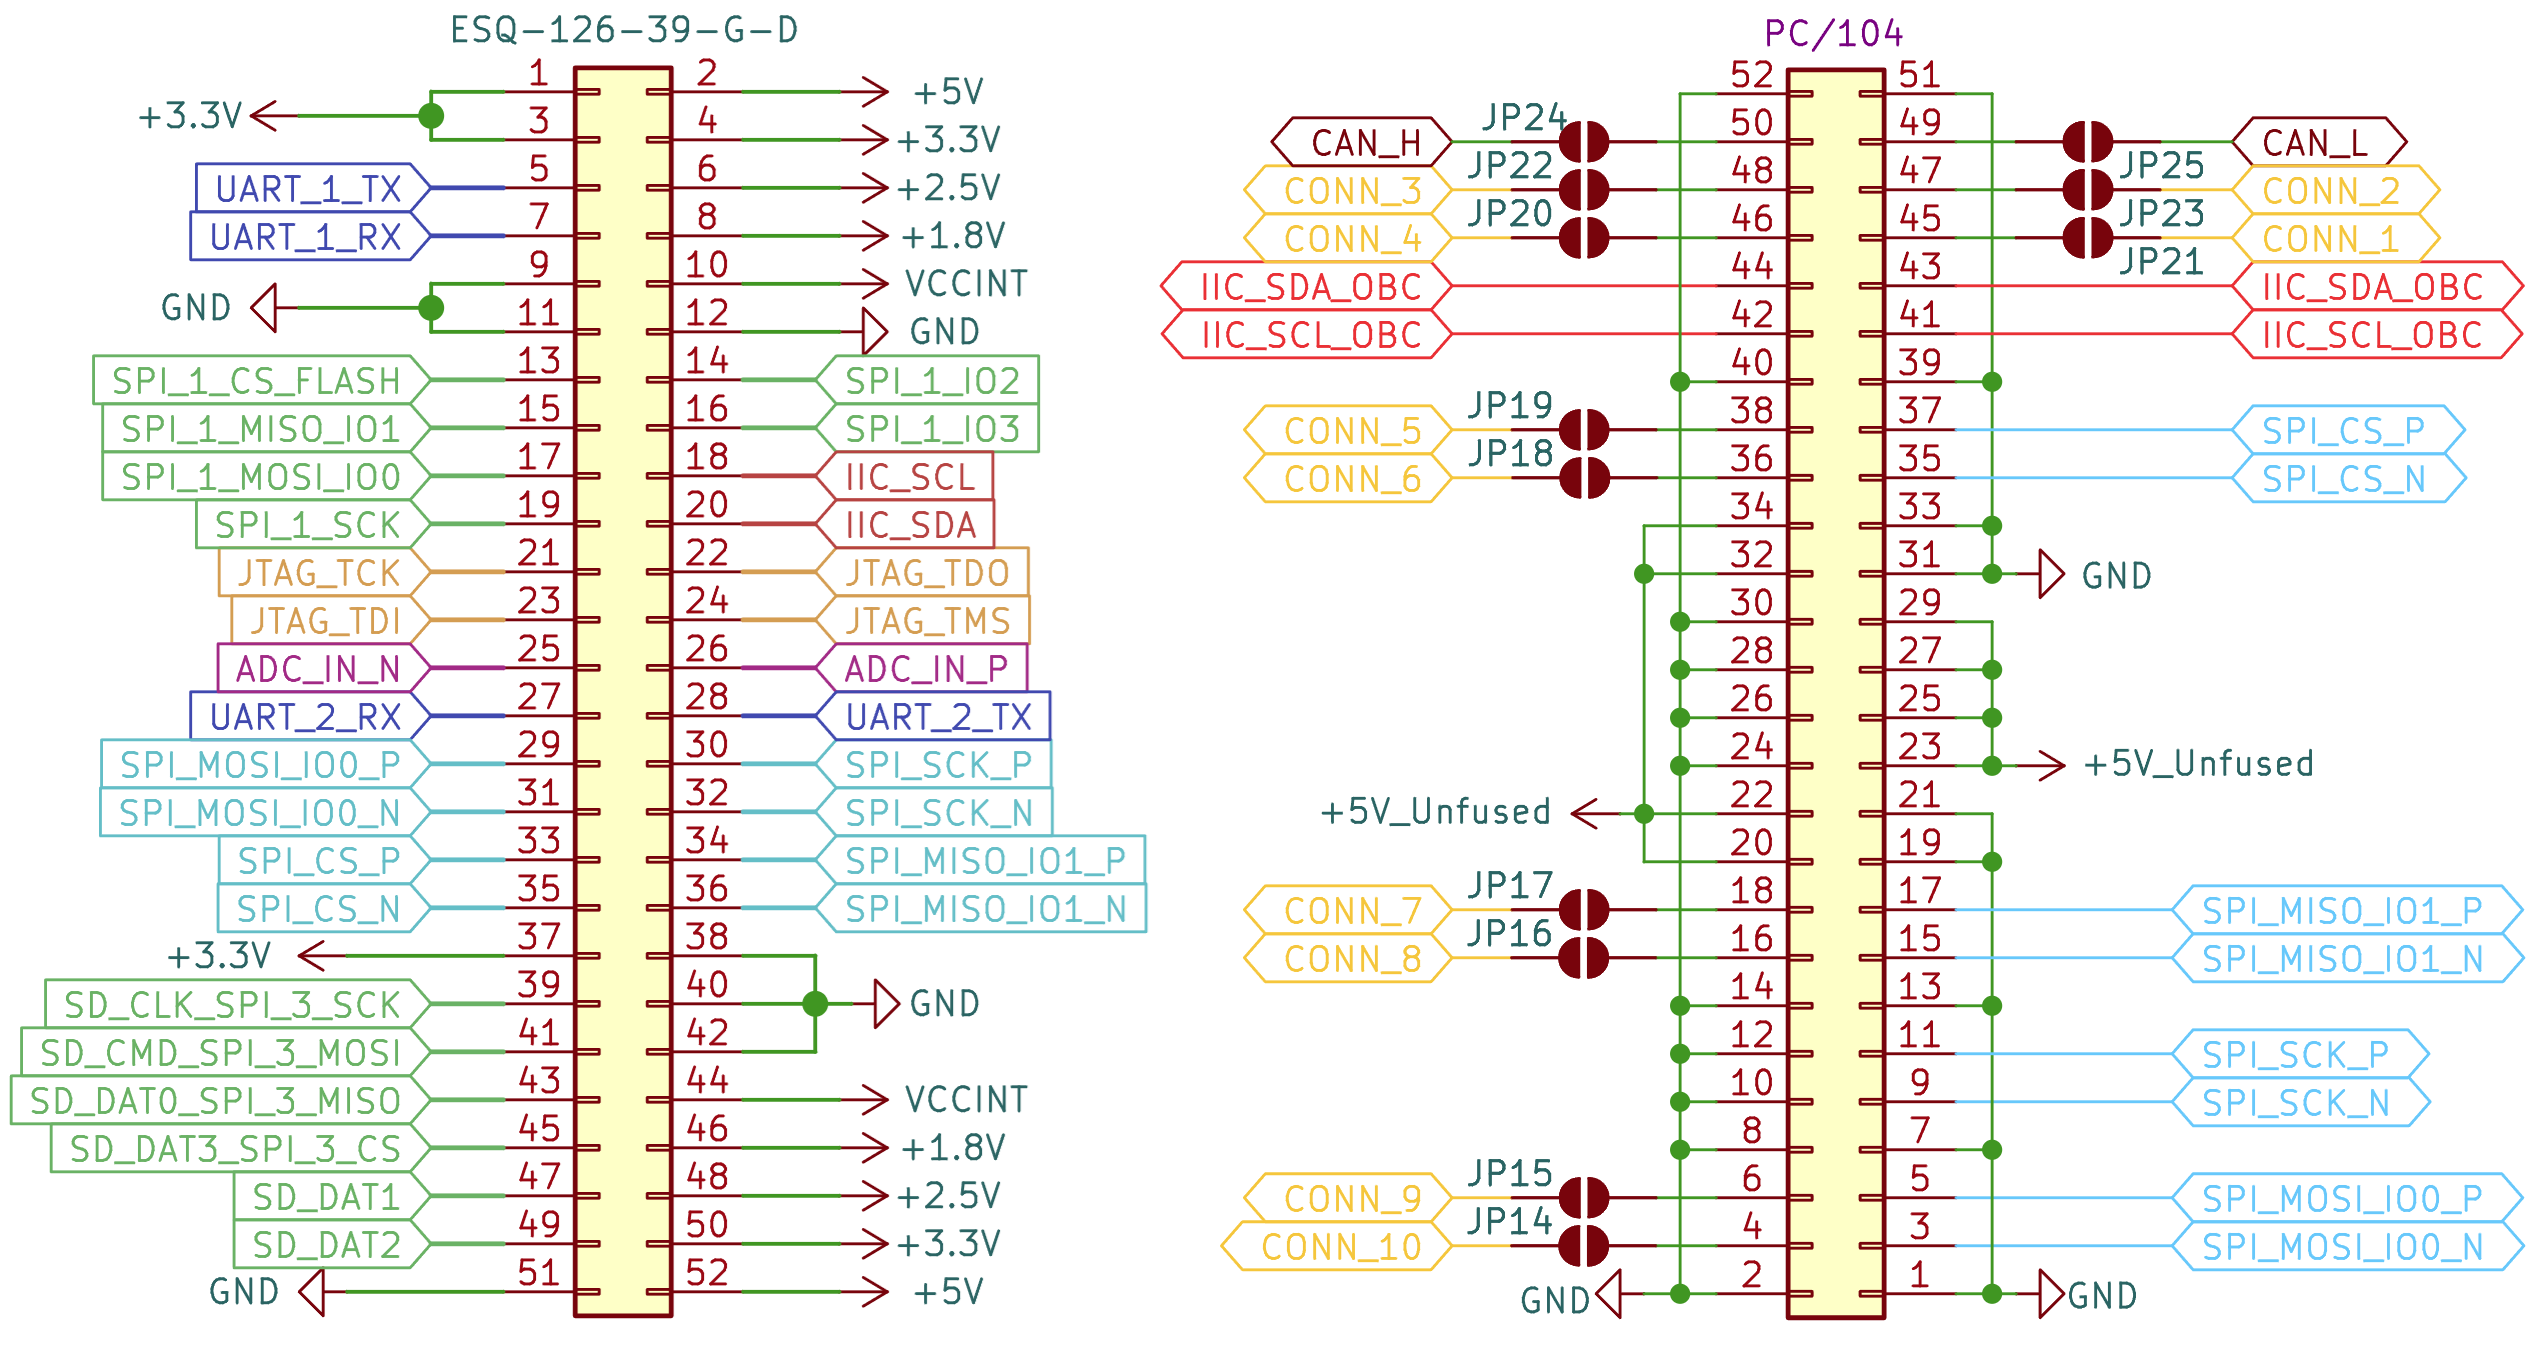
\includegraphics[width=\columnwidth]{./Images/hw_schematic_pc104.png}
    \caption{Pinout-ul conectorului PC/104 pentru cele două versiuni ale plăcii AICoRS.}%
    \label{fig:hw_schematic_pc104}
\end{figure}

\section{Diferențele aduse celei de a două versiuni ale PCB-ului}
Trecerea de la prima versiune a \gls{pcb}-ului, concepută ca prototip pentru testarea circuitelor și sistemelor, precum și pentru identificarea problemelor funcționale, la versiunea a doua, menită a fi perfect funcțională și destinată integrării finale în nanosatelit, a necesitat modificări substanțiale la nivelul schemei electrice. Aceste modificări au constat atât în eliminarea sistemelor temporare de test, cât și  în adăugarea unor circuite noi, menite să îmbunătățească fiabilitatea și compatibilitatea cu mediul spațial. Schema bloc a versiunii finale a plăcii \gls{aicors} este ilustrată în Figura~\ref{fig:hw_pcb_v2_diagram}, unde blocurile colorate în verde reprezintă circuite noi introduse, rezultate în urma concluziilor desprinse din testarea primei versiuni.

\begin{figure}[ht!]
    \centering
    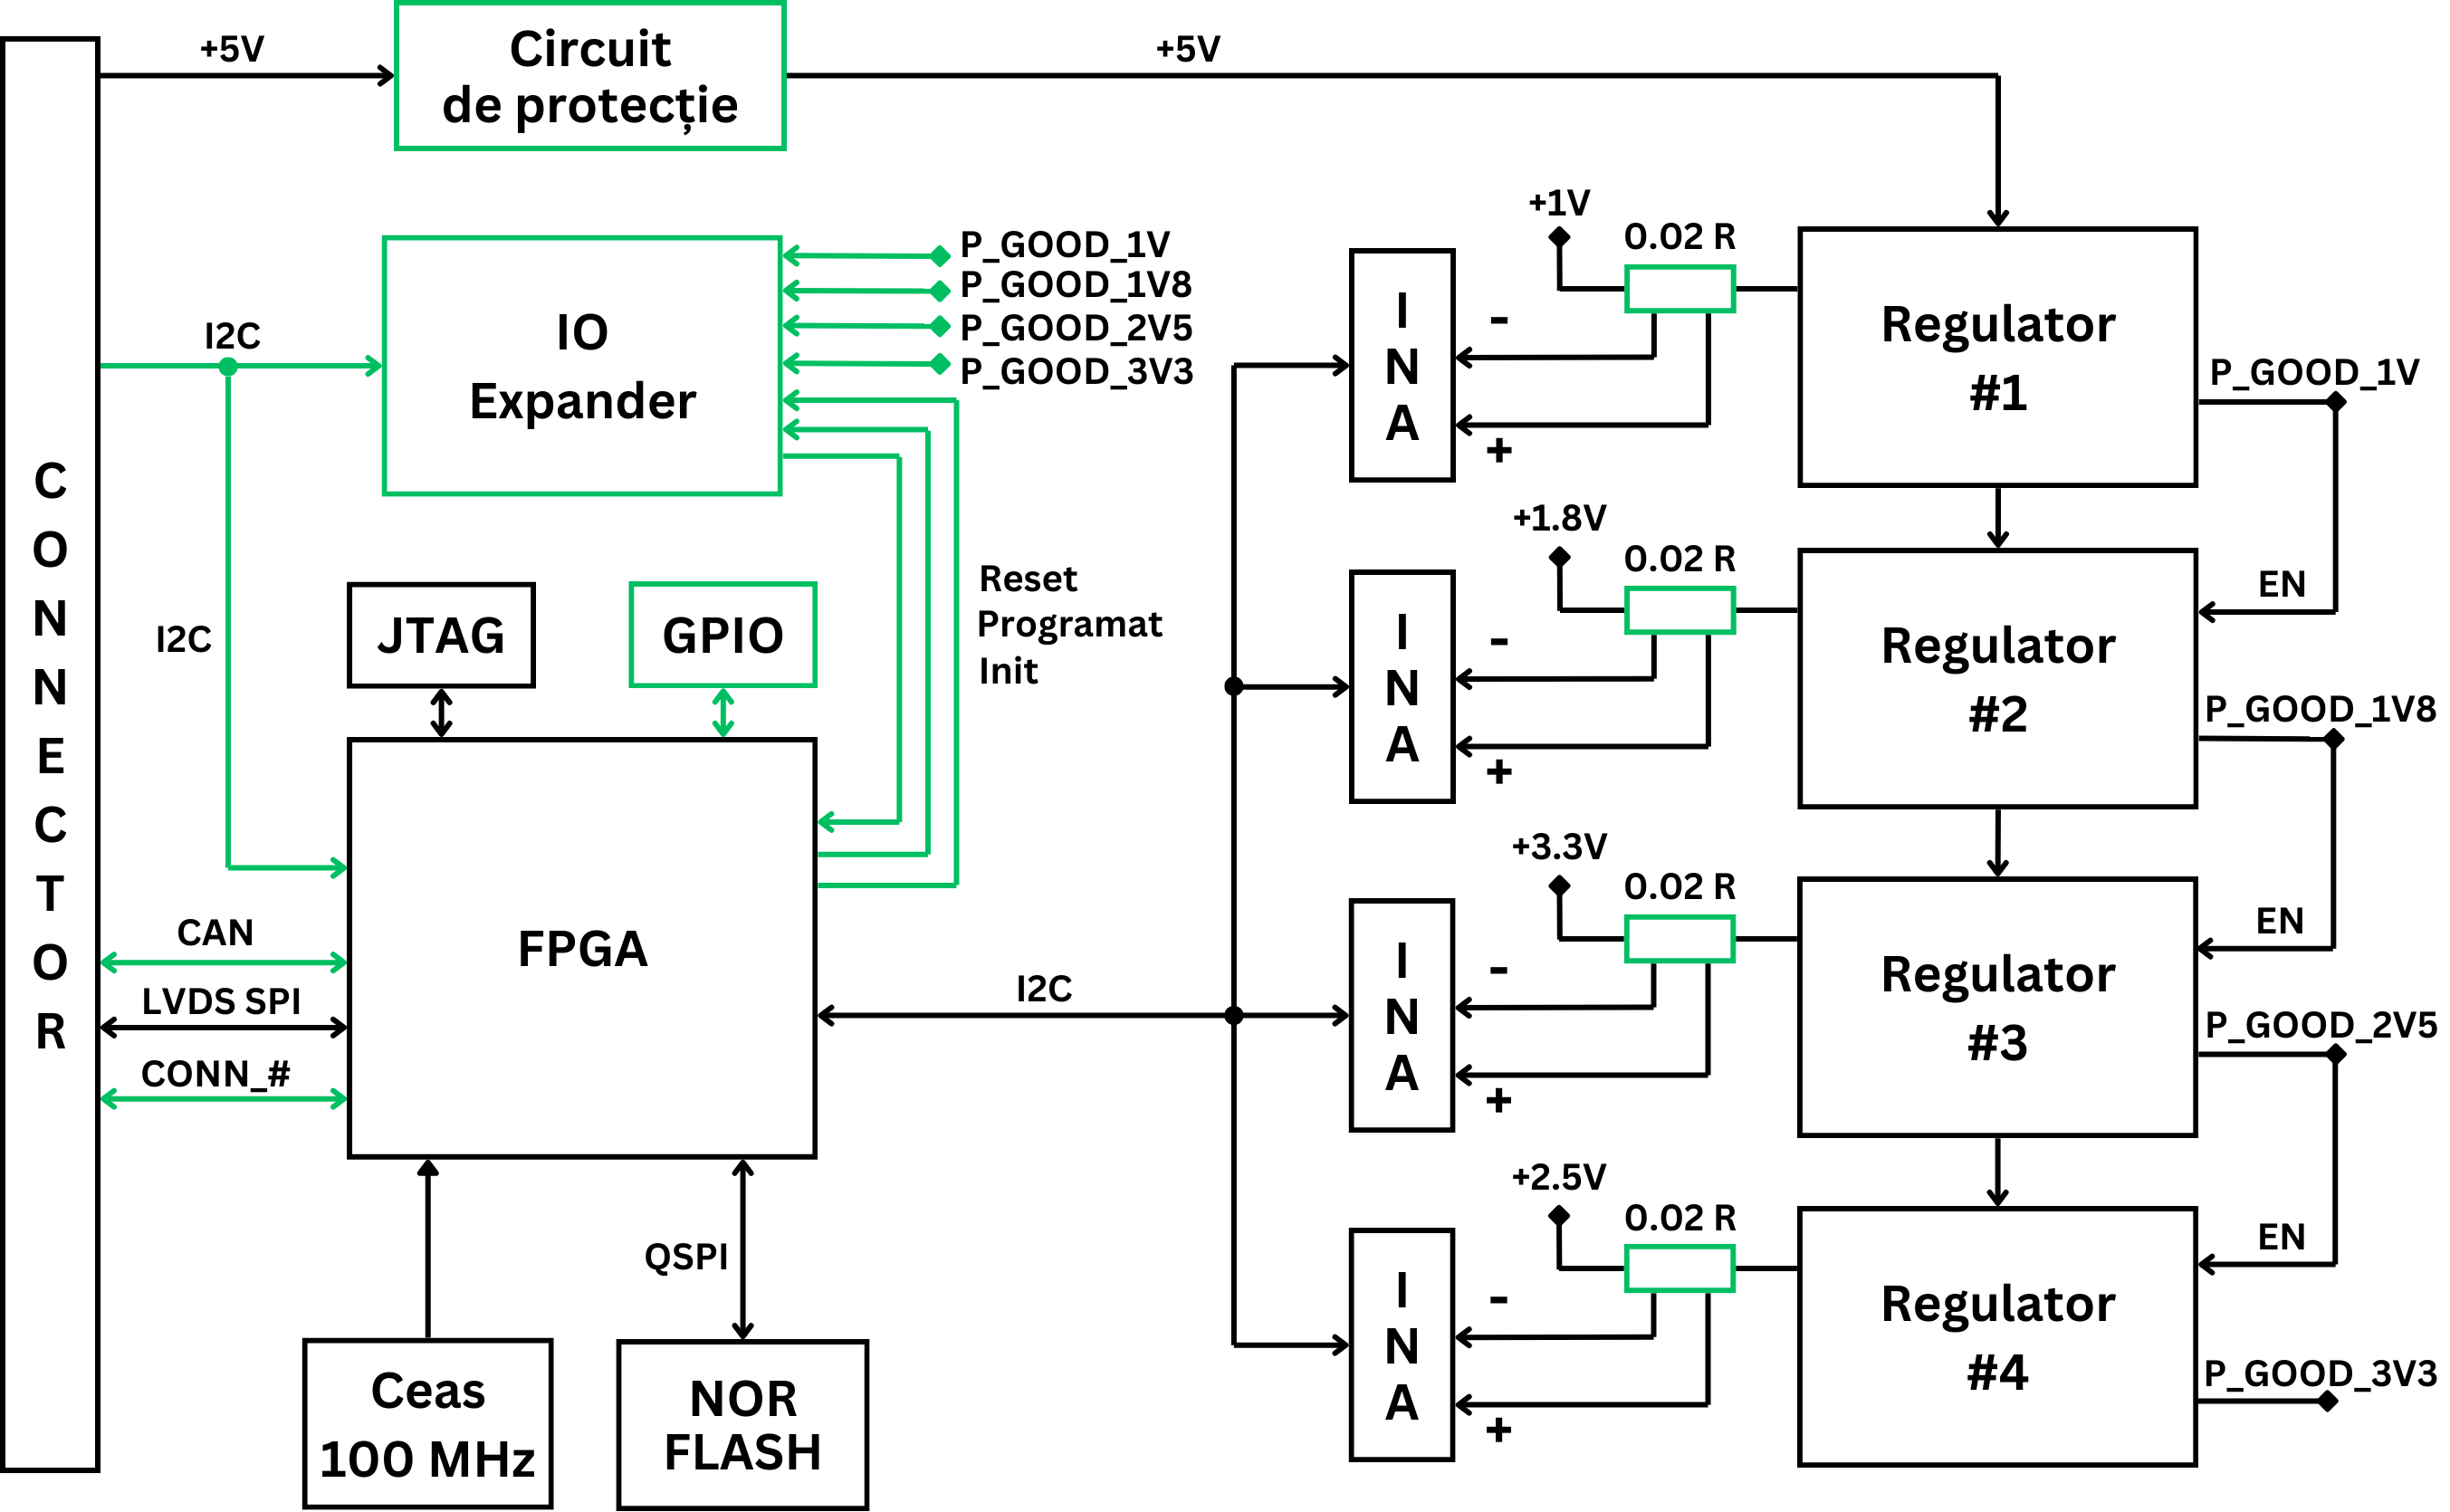
\includegraphics[width=\columnwidth]{./Images/hw_pcb_v2_diagram.png}
    \caption{Schema bloc a celei de a doua versiuni a PCB-ului AICoRS.}%
    \label{fig:hw_pcb_v2_diagram}
\end{figure}

Dintre acestea, circuitele de protecție de la interfața cu \gls{obc}-ul: conectorul PC/104, și cipul \gls{io} Expander controlat prin \gls{i2c}, vor fi detaliate în secțiunile următoare, datorită complexității lor ridicate. Principalele modificări realizate în această etapă, atât la nivel de alimentare și rutare a semnalelor, cât și în ceea ce privește protecția și testabilitatea plăcii, sunt următoarele:
\begin{itemize}\setlength\itemsep{0.2em}
    \item Eliminarea conectorului Micro-\gls{usb} și a convertorului \gls{usb} la \gls{jtag}/\gls{uart}.
    \item Eliminarea întrerupătorului și a LED-ului de alimentare.
    \item Eliminarea conectorului pentru card Micro-SD.
    \item Eliminarea perechii de pini analogici proveniți de la \gls{fpga}.
    \item Eliminarea LED-urilor atașate regulatoarelor de tensiune.
    \item Eliminarea LED-ului și butonului conectate la pinii de status ai \gls{fpga}-ului. 
    \item Eliminarea mărgelelor de ferită de la regulatoarele de tensiune, deoarece testele au arătat că poziționarea lor incorectă genera zgomot suplimentar.
    \item Înlocuirea rezistorilor de shunt de la 0.003 \(\Omega\) cu unii de 0.02 \(\Omega\). Astfel, se permite calibrarea senzorilor de curent INA219 pentru un interval de măsură mai mic, dar cu sensibilitatea și rezoluția crescute.
    \item Introducerea unui conector \gls{pmod} (tip header cu două rânduri a câte șase pini), care adaugă opt pini \gls{gpio} de 3.3 V conectați la \gls{fpga}, utili pentru testare și extinderea funcționalităților.
    \item Adăugarea unui conector suplimentar de tip header cu două rânduri a câte șase pini pentru a ușura accesul la toate liniile de alimentare de pe \gls{pcb}.
    \item Introducerea a zece pini \gls{gpio} conectați la conectorul PC/104 și la \gls{fpga}, care pot fi folosiți în testarea \gls{pcb}-ului și în alte aplicații, atunci când nu sunt utilizați de alte module.
    \item Eliminarea punctelor de test redundante și adăugarea a unor puncte de test noi, dedicate semnalelor de interes.
\end{itemize}

O îmbunătățire majoră a constat și în optimizarea procesului de layout și rutare a plăcii, care a permis reducerea numărului de straturi necesare de la șase la patru. Planurile de alimentare au fost comasate într-un singur strat, iar planul inferior de masă a fost eliminat, conform structurii prezentate în Tabelul~\ref{tab:hw_pcb_v2_layers}. Pentru a nu introduce probleme legate de integritatea semnalului, toate liniile sensibile au fost rutate pe stratul superior, acesta beneficiind de un plan de masă uniform de referință, spre deosebire de stratul inferior, unde efectul ecranării este mult diminuat.

\begin{table}[h!]
    \footnotesize
    \centering
    \renewcommand{\arraystretch}{1.6} 
    \caption{Stackup-ul a celei de a doua versiuni a PCB-ului.}%
    \label{tab:hw_pcb_v2_layers}
    \begin{tabular}{C{1.2cm} L{2cm} C{3.2cm} L{3.5cm} L{2.5cm} C{2cm}}
		\toprule
			\textbf{Nr.} & 
            \textbf{Nume} & 
            \textbf{Grosime [mm]} & 
            \textbf{Rol} & 
            \textbf{Material} & 
            \textbf{Permitivitate relativă}\\
		\midrule
		    1 & Top           & 0.035  & Semnal                & Cupru     & ---  \\
		    2 & Dielectric 1  & 0.210  & PrePreg               & FR4 7628  & 4.4  \\
		    3 & Interior 1    & 0.0152 & Plan de masă          & Cupru     & ---  \\
		    4 & Dielectric 2  & 1.065  & Nucleu                & FR4       & 4.6  \\
		    5 & Interior 2    & 0.0152 & Plan de alimentare    & Cupru     & ---  \\
		    6 & Dielectric 3  & 0.210  & PrePreg               & FR4 7628  & 4.4  \\
		    7 & Bottom        & 0.035  & Semnal                & Cupru     & ---  \\
		\bottomrule
    \end{tabular}
\end{table}

\subsection[I2C IO expander]{I\textsuperscript{2}C IO expander}
Pentru a permite \gls{obc}-ului să controleze și să monitorizeze anumite semnale de status fără ca \gls{fpga}-ul să fie programat, a fost introdus cipul TCA6408ARGTR\cite{i2c_expander_datasheet}, un \gls{io} Expander pe 8 biți cu interfață \gls{i2c}. Acesta este conectat la un bus \gls{i2c} distinct de cel utilizat de senzorii INA219, fiind legat la \gls{fpga} și, prin conectorul PC/104, la \gls{obc}. În această configurație, \gls{obc}-ul nanosatelitului acționează ca master, în timp ce dispozitivul \gls{fpga} și cipul \gls{io} Expander funcționează ca slave.

Semnalele \gls{io} asociate acestui dispozitiv includ pinii P\_GOOD ai celor patru regulatoare de tensiune, pinii \textit{DONE}, \textit{INIT} și \textit{PROGRAM\_B} ai \gls{fpga}-ului, precum și pinul de reset propriu cipului. La inițializare, dispozitivul configurează toți pinii ca intrări, prevenind astfel orice conflict electric între semnale. Primii patru pini acționează ca intrări și sunt utilizați pentru monitorizarea regulatoarelor de tensiune și pentru identificarea eventualelor defecțiuni, iar ceilalți trei pini conectați la \gls{fpga} pot fi folosiți pentru urmărirea procesului de configurare, resetarea dispozitivului (prin asertarea valorii 0 pe pinul \textit{PROGRAM\_B}) sau amânarea configur[rii] (prin menținerea pinului \textit{INIT} în 0). Pinul de reset al cipului este conectat la unul dintre pinii săi \gls{io}, permițând resetarea acestuia direct prin interfața \gls{i2c}, fără circuite externe suplimentare.

Magistrala \gls{i2c} aferentă acestui cip este fizic separată de magistrala utilizată de senzorii INA219, deoarece, în cazul celei din urmă, masterul este \gls{fpga}-ul. Dacă se dorește citirea senzorilor INA219 de către \gls{obc}, cele două magistrale pot fi interconectate prin intermediul a doi jumperi, permițând astfel comunicarea tuturor dispozitivelor cu \gls{obc}-ul. Dacă însă aceste două magistrale sunt conectate între ele, rezistorii de pull-up aferenți liniilor SDA și SCL trebuie îndepărtați, deoarece aceștia sunt deja prezenți pe \gls{pcb}-ul masterului, adică \gls{obc}-ul.

\subsection{Circuite de protecție}
Pentru a proteja \gls{pcb}-ul împotriva anomaliilor electrice provenite din mediul extern, precum supratensiuni, supracurenți, vârfuri tranzitorii sau alte evenimente neprevăzute, au fost implementate o serie de circuite de protecție asupra semnalelor care intră în \gls{pcb} prin conectorul PC/104. Acestea sunt ilustrate în Figura~\ref{fig:hw_schematic_prot_circuits}.

În partea stânga-sus a figurii este prezentat circuitul de protecție pentru linia de alimentare de 5 V. Între conectorul PC/104 și regulatoarele de tensiune este plasată o siguranță PTC resetabilă (descrisă anterior) și o diodă \gls{tvs} unidirecțională, destinată protecției împotriva supratensiunilor și impulsurilor tranzitorii. Aceasta este conectată în polarizare inversă și are o tensiune de străpungere între 6.4 --- 7 V, cu o putere maximă disipabilă la impuls de 400 W.

Pentru interfața \gls{i2c} au fost utilizate două diode \gls{tvs} bidirecționale, dedicate protecției la descărcării electrostatice (ESD). Acestea sunt conectate între liniile SDA, respectiv SCL, și masă, având tensiunea nominală de 3.3 V și o tensiune de străpungere de 5 V. Capacitatea maximă de 15 pF este suficient de mică pentru a nu afecta semnalele din această interfață, iar tensiunea maximă de protecție este de 18 kV.

Pentru interfața \gls{lvds} \gls{spi} au fost utilizate diode \gls{tvs} de protecție ESD similare celor folosite pentru interfața \gls{i2c}, cu diferența că acestea dispun de două canale, caracteristică necesară pentru liniile diferențiale ale acestei interfețe. Diodele au o tensiune nominală de operare de 3.6 V și o tensiune de străpungere de 4.5 V, fiind compatibile cu semnalele \gls{lvds} și conforme cu standardele IEC 61000-4-5 pentru protecție la supratensiune și IEC 61000-4-2 pentru protecție ESD.\@

\begin{figure}[ht!]
    \centering
    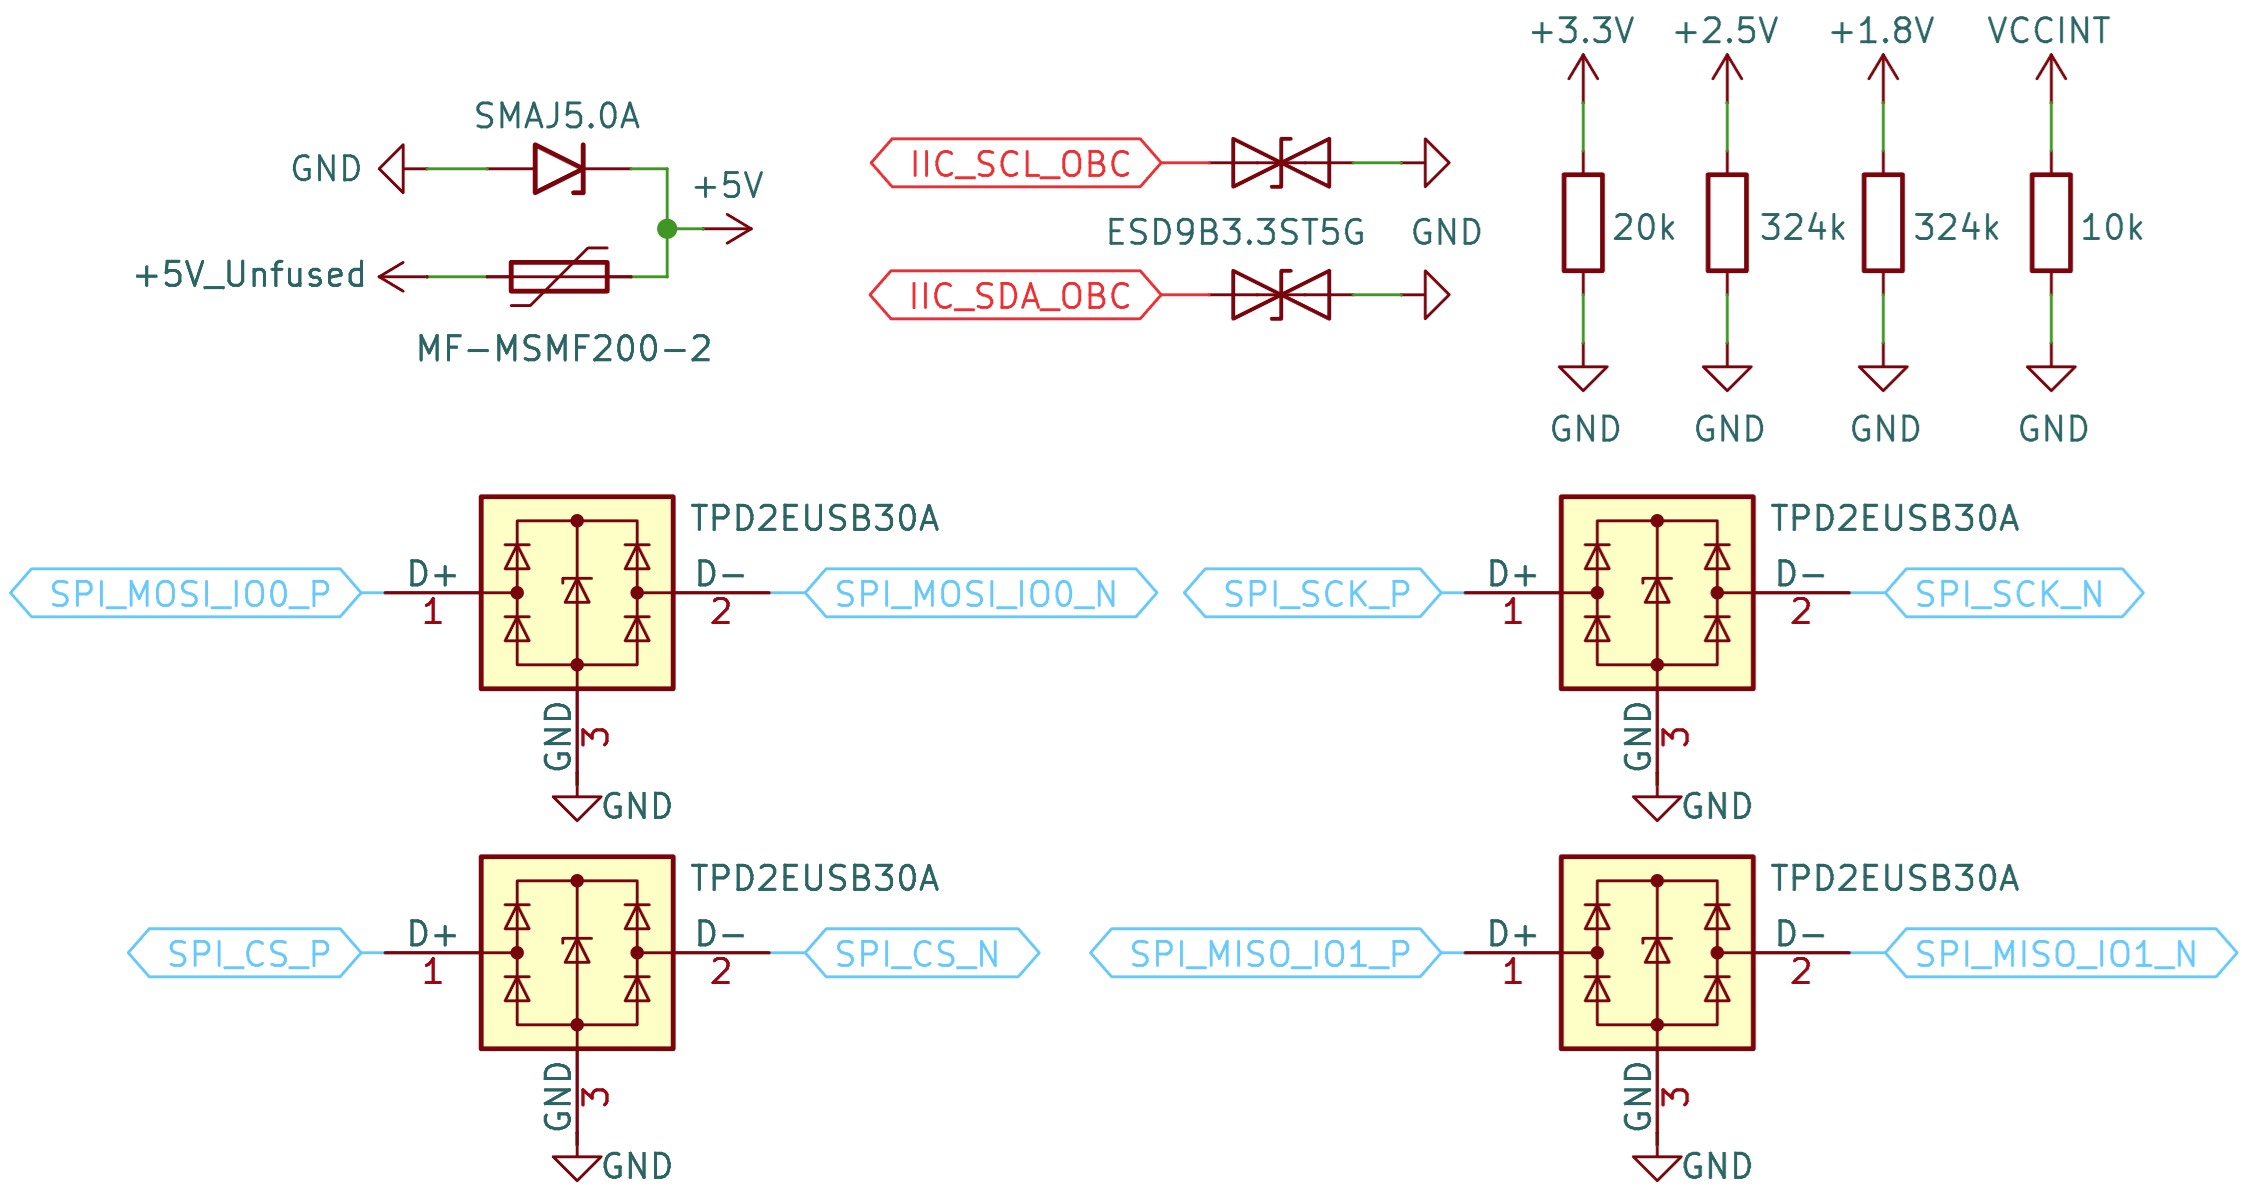
\includegraphics[width=0.8\columnwidth]{./Images/hw_schematic_prot_circuits.png}
    \caption{Schema electrică a circuitelor de protecție de pe a PCB-ul AICoRS.}%
    \label{fig:hw_schematic_prot_circuits}
\end{figure}

Din cauza capacității totale ridicate a liniilor de alimentare și rezistenței de scurgere relativ mici, la întreruperea alimentării acestea pot rămâne încărcate pentru o perioadă considerabilă de timp, fenomen ce poate genera erori în funcționarea \gls{fpga}-ului și a altor dispozitive. Pentru a preveni astfel de situații, au fost introduși rezistori de pull-down pe fiecare dintre cele patru linii de alimentare. Valorile acestora au fost alese astfel încât liniile să se descarce suficient de rapid, menținând în același timp un curent de scurgere redus. Tabelul~\ref{tab:hw_discharge_times} prezintă caracteristicile fiecărei tensiuni: capacitatea totală, estimată prin însumarea tuturor condensatorilor conectați, timpul de descărcare până la sub 1\% din tensiunea inițială, calculat conform relației \(T \approx 5RC\), rezistorul de pull-down 
ales și puterea disipată de acesta, determinată cu formula \(P = U^2 / R\).

\begin{table}[h!]
    \footnotesize
    \centering
    \renewcommand{\arraystretch}{1.6} 
    \caption{Timpii de descărcare și rezistențele calculate pentru liniile de tensiune.}%
    \label{tab:hw_discharge_times}
    \begin{tabular}{C{2.3cm} C{3cm} C{3.5cm} C{3cm} C{3cm}}
		\toprule
            \textbf{Tensiune} & 
            \textbf{Capacitatea totală} & 
            \textbf{Timp de descărcare*} & 
            \textbf{Rezistență necesară} & 
            \textbf{Putere disipată}\\
		\midrule
            1.0 V & 1.0 mF     & 50 s & 10 k$\Omega$  & 0.10 mW \\
            1.8 V & 40 $\mu$F  & 65 s & 324 k$\Omega$ & 0.01 mW \\
            2.5 V & 40 $\mu$F  & 65 s & 324 k$\Omega$ & 0.02 mW \\
            3.3 V & 670 $\mu$F & 67 s & 20 k$\Omega$  & 0.54 mW \\
        \bottomrule
        \multicolumn{5}{l}{\footnotesize * Calculat pentru a descărca linia sub 1\% din tensiunea inițială.} \\
    \end{tabular}
\end{table}

\section{Concluzii}
Scopul principal al dezvoltării plăcii \gls{aicors} a fost: (i) furnizarea unui suport fizic pentru dispozitivul \gls{fpga}, (ii) asigurarea unei alimentări stabile pentru \gls{fpga} și pentru celelalte componente prin cele patru tensiuni de alimentare, (iii) oferirea unei structuri direct integrabile în nanosatelitul țintă și (iv) oferirea de protecție și robustețe în fața mediului spațial extrem. Aceste obiective au fost realizate prin proiectarea și fabricarea celor două versiuni de \gls{pcb}, ambele asamblate cu succes utilizând serviciile JLCPCB.\@ Proiecția de deasupra a celor două versiuni este prezentată în Figura~\ref{fig:hw_pcbs_horizontal}, prima versiune fiind în stânga, iar cea de-a doua în dreapta. Au fost produse trei exemplare asamblate și două exemplare fără componente. Toate piesele au fost selectate de echipa de dezvoltare și obținute și depozitate de JLCPCB. Ulterior, aceste componente au fost folosite pentru asamblare, excesul nefolosit fiind revândut.

\begin{figure}[ht!]
    \centering
    \includegraphics[width=\columnwidth]{./Images/hw_pcbs_horizontal.png}
    \caption{Cele două versiuni ale PCB-ului AICoRS.}%
    \label{fig:hw_pcbs_horizontal}
\end{figure}

Procesul de proiectare și testare a primei versiuni a permis dezvoltarea unor strategii de rutare și plasare a componentelor mai optime, precum și identificarea și rezolvarea diverselor probleme legate de circuitele electrice. Principalele îmbunătățiri aduse celei de-a doua versiuni includ: 
\begin{itemize}
    \item Reducerea numărului de straturi de la șase la patru prin optimizarea procesului de rutare al planurilor de tensiune.
    \item Eficientizarea rutării traseelor și a selecției pinilor folosiți ai \gls{fpga}-ului, ceea ce reduce vulnerabilitatea semnalelor la zgomot și crește eficiența rutării.
    \item Introducerea unui cip \gls{io} Expander pentru monitorizarea și resetarea \gls{pcb}-ului.
    \item Eliminarea tuturor componentelor de testare și depanare neesențiale pentru a minimiza consumul de energie.
    \item Concretizarea formei generale a plăcii și poziționarea componentelor critice pentru compatibilitate cu nanosatelitul țintă.
    \item Adăugarea circuitelor de protecție pentru semnalele de intrare și ieșire ale plăcii.
\end{itemize}
Straturile superioare și inferioare ale versiunii finale a plăcii \gls{aicors} sunt prezentate în Figura~\ref{fig:hw_layout_horizontal}. Se observă în special rutarea semnalelor de la \gls{fpga} către conectori, izolarea și separarea circuitelor regulatoare de tensiune de restul sistemelor, precum și egalizarea lungimilor traseelor pentru semnalele importante.

\begin{figure}[ht!]
    \centering
    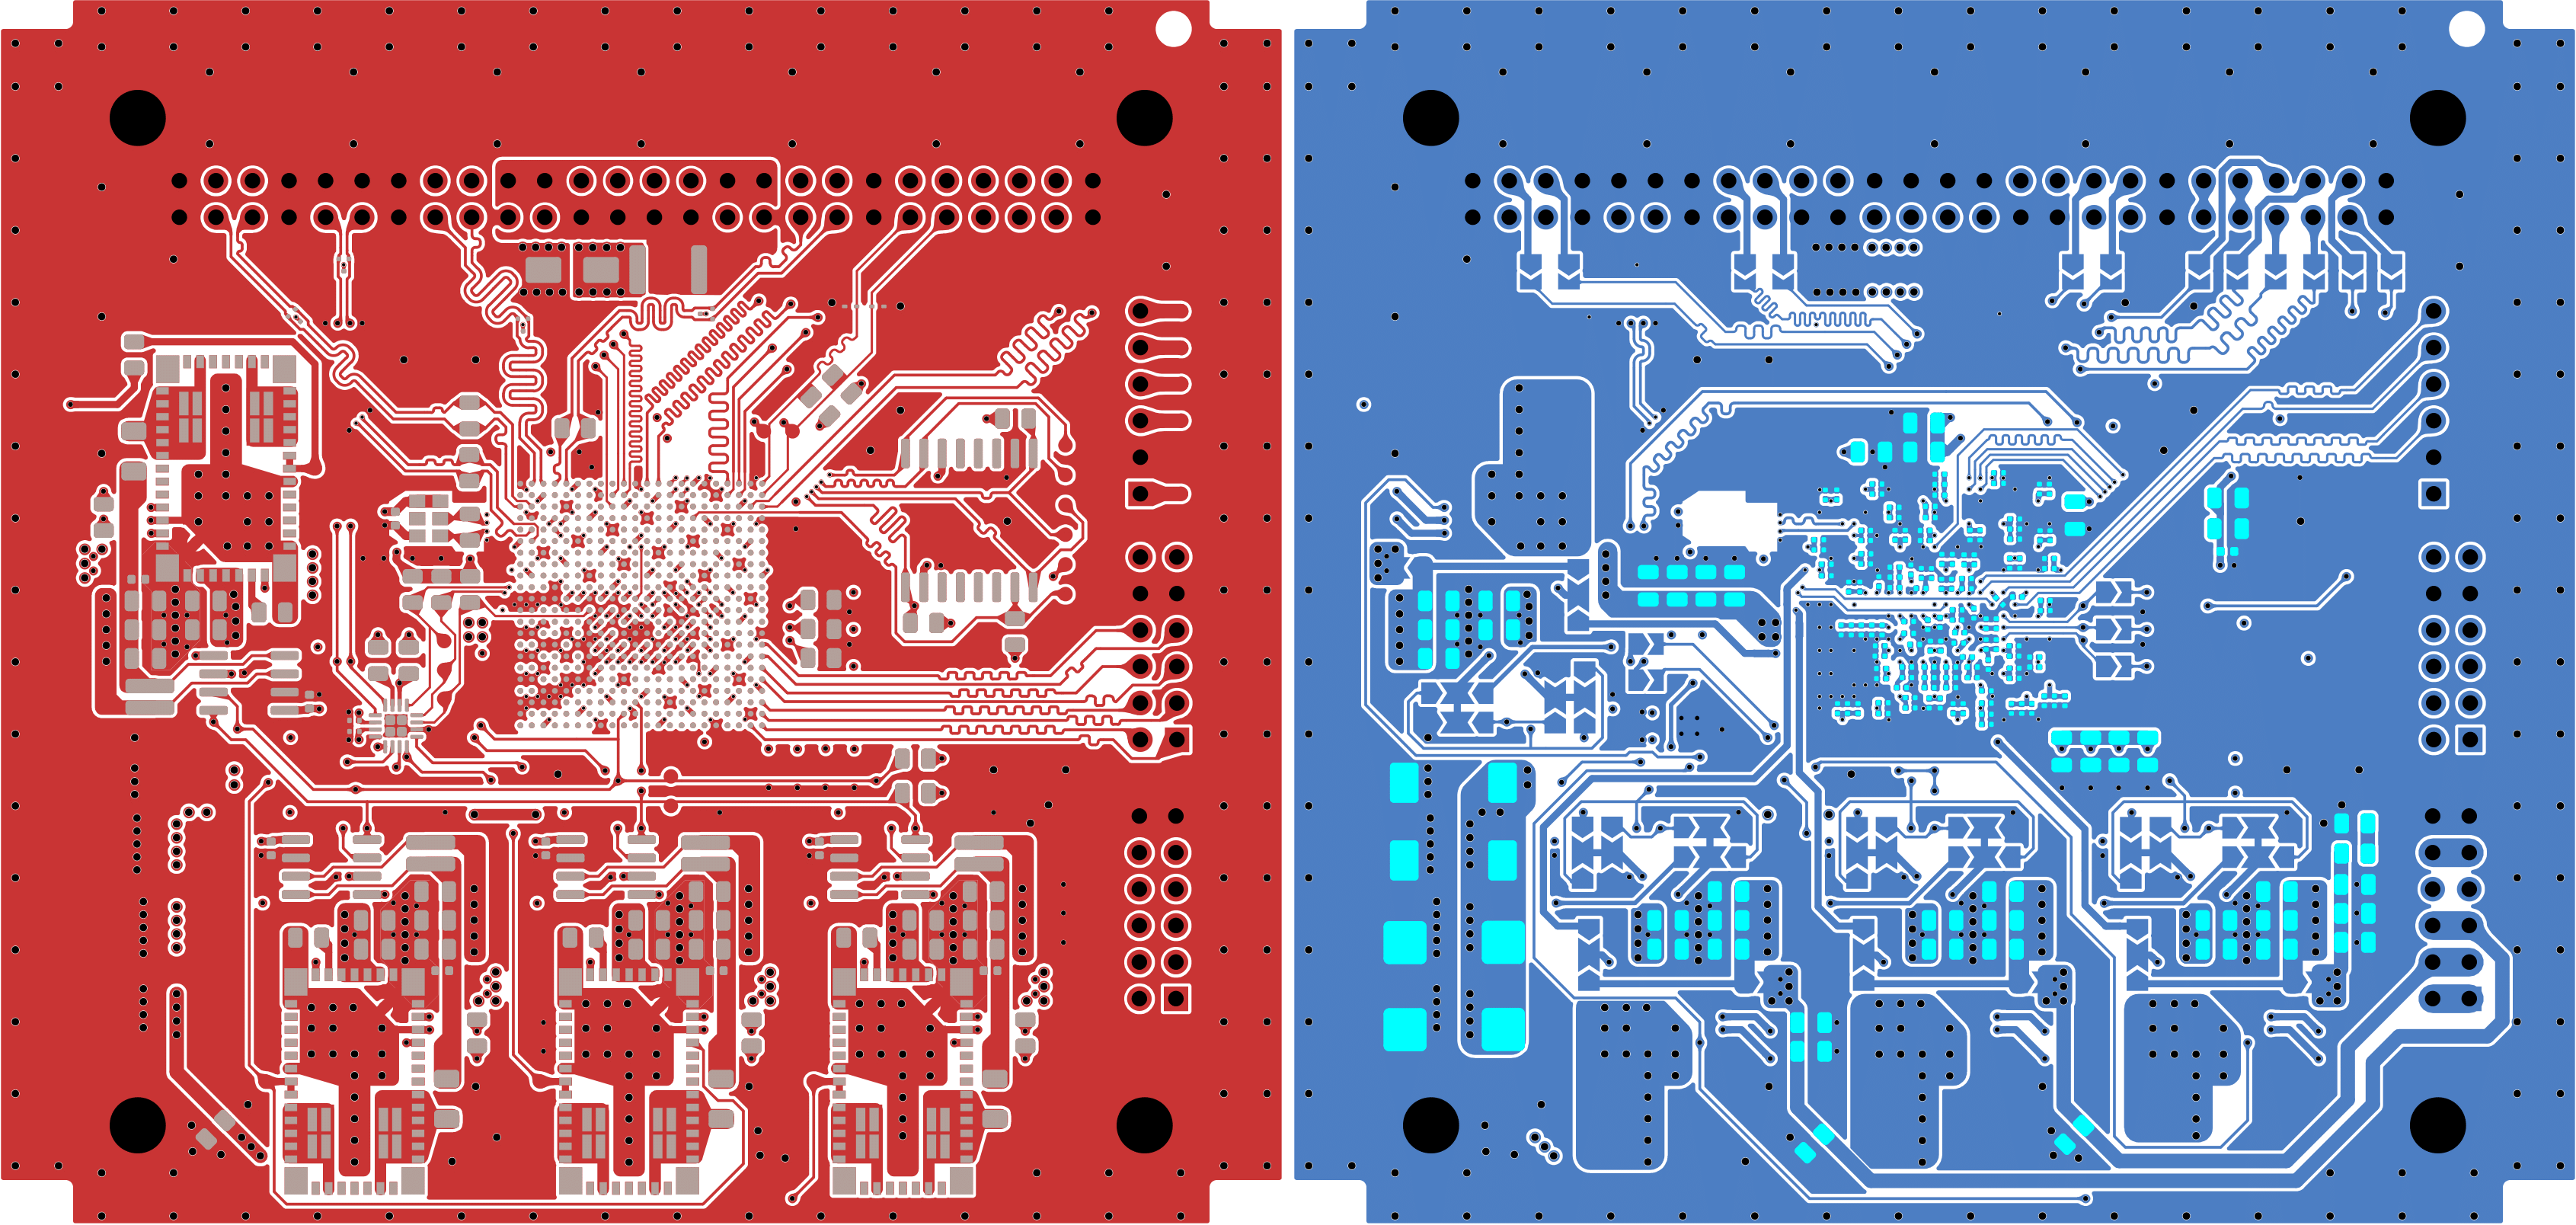
\includegraphics[width=\columnwidth]{./Images/hw_layout_horizontal.png}
    \caption{Straturile exterioare (Top și Bottom) ale versiunii finale a PCB-ului AICoRS.}%
    \label{fig:hw_layout_horizontal}
\end{figure}

Deși proiectată inițial pentru aplicația \gls{aicors}, placa a fost concepută având în vedere reutilizarea sa și în alte activități. Jumperii care permit conectarea \gls{fpga}-ului la toți pinii conectorului PC/104, prezența unui conector \gls{pmod} suplimentar, precum și alimentarea de la o singură tensiune de 5 V fac posibilă utilizarea acestor \gls{pcb}-uri ca plăci de dezvoltare \gls{fpga} în scopuri didactice sau în scopuri academice, precum și ca senzori de radiație cosmică în alți nanosateliți sau în centre de cercetare. Aceste plăci pot fi integrate în cadrul unor laboratoare care oferă acces la plăci de dezvoltare cu \gls{fpga} ce pot fi folosite pentru predarea dezvoltării hardware, sau chiar programării embedded, prin pre-configurarea cu un microprocesor MicroBlaze. Pot fi utilizate în mediul academic și de cercetare, fie prin integrarea în alte misiuni spațiale cu cerințe similare, fie în centre de testare și radiație terestre, precum Organizația Europeană pentru Cercetare Nucleară (CERN) sau Laboratorul Național Los Alamos (LANL). Dacă placa își dovedește robustețea și fiabilitatea în cadrul misiunii actuale, aceasta ar putea fi ulterior folosită în scopuri didactice sau industriale, ca exemplu de proiectare rezistentă la radiație, atât la nivelul \gls{pcb}-ului suport, cât și al implementării hardware.

Dacă aceste direcții reprezintă domenii active de interes, placa \gls{aicors} poate fi îmbunătățită în versiunile viitoare prin modificarea conectorului PC/104 sau prin integrarea unor conectori suplimentari de mare viteză, adăugarea unor memorii externe pentru stocarea datelor sau pentru detectarea radiației, precum și prin includerea unor interfețe de comunicație de viteză ridicată direct în \gls{fpga}. De asemenea, ar putea fi adăugat unui microprocesor care să lucreze în tandem cu \gls{fpga}-ul, facilitând implementarea unor aplicații complexe, dificil de realizat în limbaj \gls{hdl}. 

Pentru a încheia această parte a lucrării, în Figura~\ref{fig:hw_3d_render} se ilustrează modelul 3D al plăcii \gls{aicors}. Această reprezentare reunește toate etapele de proiectare și evidențiază produsul final obținut, oferind o imagine de ansamblu ușor de înțeles asupra sistemului dezvoltat.

\begin{figure}[ht!]
    \centering
    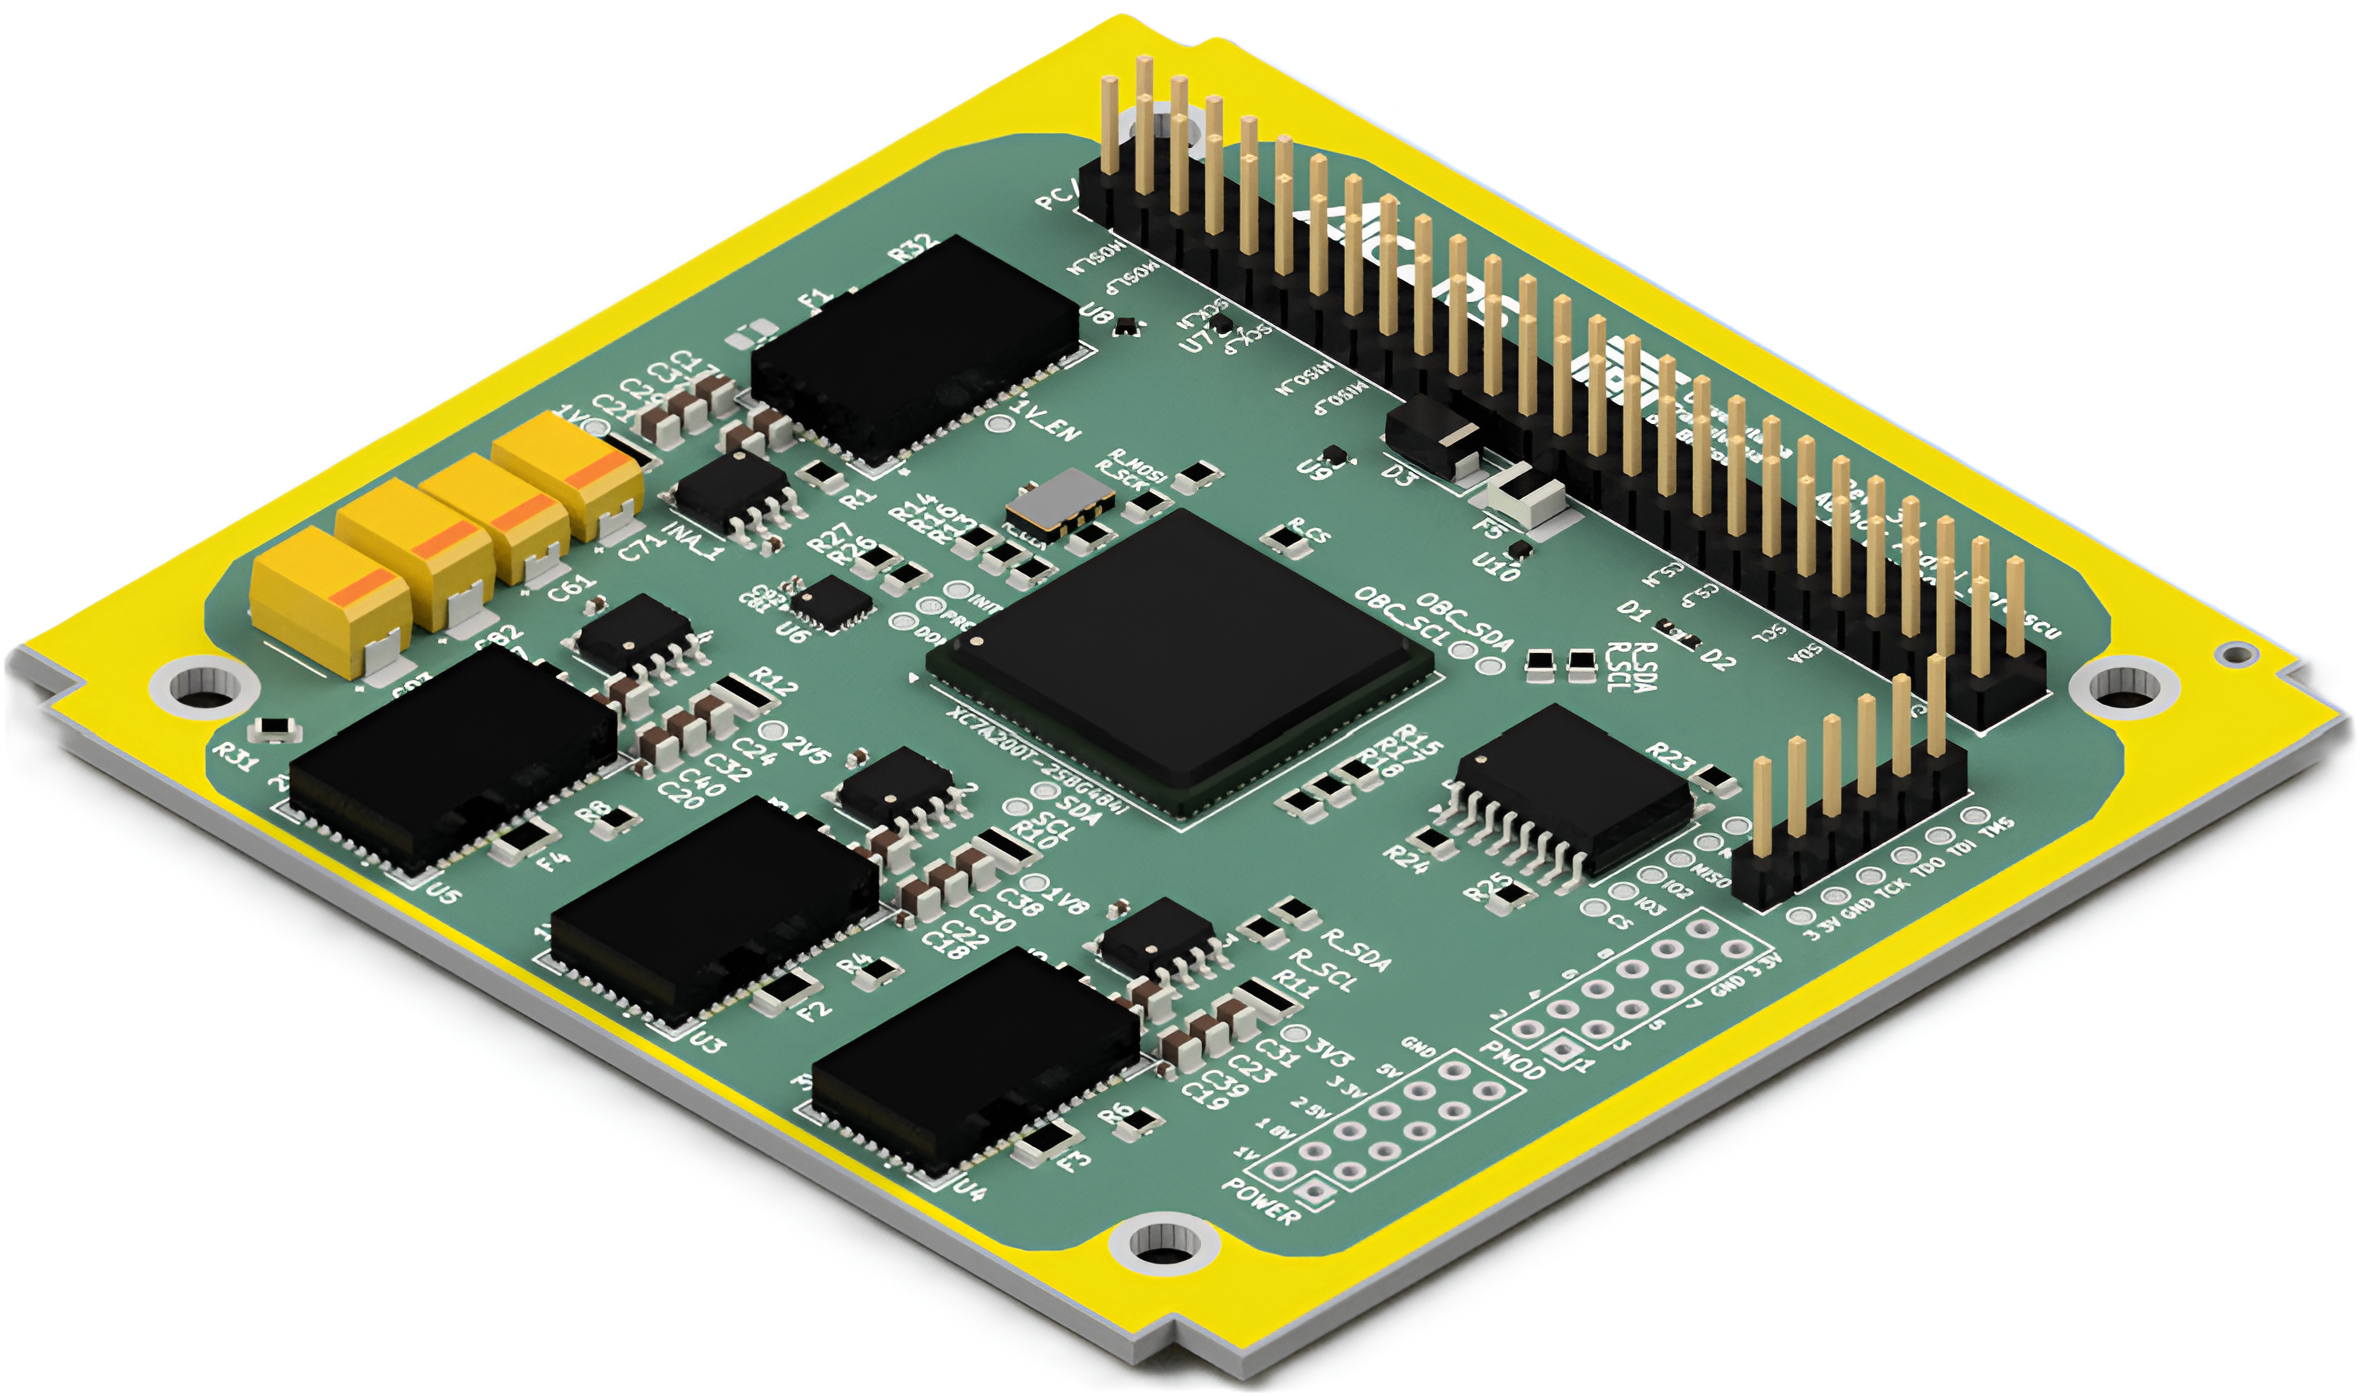
\includegraphics[width=0.8\columnwidth]{./Images/hw_3d_render.png}
    \caption{Modelul 3D al celei de-a doua versiune a plăcii AICoRS.}%
    \label{fig:hw_3d_render}
\end{figure}

În continuare, este prezentat procesul de testare și validare a plăcii \gls{aicors}, care include simulările software ale configurării Verilog, verificarea funcționalității \gls{pcb}-ului și a sistemelor integrate pe acesta, precum și validarea ansamblului complet prin conectarea la \gls{obc} și testarea interfețelor de comunicație și a conexiunilor fizice. Secțiunea următoare va aborda testele de consum, simulările comportamentale, verificările privind integritatea semnalului și a alimentării, precum și teste de comunicație între \gls{fpga}, \gls{obc} și celelalte dispozitive de pe \gls{pcb}.

% ---------------------------------------------------------------

\chapter{Testarea și validarea proiectului AICoRS}
Pentru a asigura funcționarea corectă și fiabilă a plăcii \gls{aicors}, atât din punct de vedere hardware, cât și software, au fost efectuate o serie de teste și proceduri de validare asupra configurării \gls{fpga}-ului și asupra \gls{pcb}-ului asociat. Aceste teste au avut ca scop confirmarea corectitudinii algoritmilor implementați și a integrității circuitelor electrice. Testele au fost realizate atât în medii de simulare software, pentru verificarea logicii și a funcționalității modulelor Verilog, cât și în medii fizice. 

Au fost utilizate instrumente dedicate pentru simulare, măsurători de consum și verificarea interfețelor de comunicație, asigurând astfel o evaluare completă a sistemului. În continuare, în Tabelul \ref{tab:ts_tests_list} sunt enumerate cele mai relevante teste și validări efectuate, împreună cu instrumentele utilizate și tipul mediului de testare (simulare și fizic). 

\begin{table}[h!]
    \footnotesize
    \centering
    \renewcommand{\arraystretch}{1.6} 
    \caption{Lista de teste efectuate pentru validarea proiectului AICoRS.}%
    \label{tab:ts_tests_list}
    \begin{tabular}{C{1cm} L{7cm} L{3cm} L{4,3cm}}
		\toprule
			\textbf{Nr.} & 
            \textbf{Denumire test} & 
            \textbf{Mediu} & 
            \textbf{Unelte folosite}\\
        \midrule
            1 & Inspecția fizică și integritatea generală a \gls{pcb}-ului 
              & Fizic 
              & Inspecție vizuală \\
            2 & Verificarea funcționării și programabilității \gls{fpga}-ului 
              & Fizic și software 
              & Vivado, multimetru \\
            3 & Testarea și validarea logicii \gls{hdl}
              & Fizic și simulare  
              & Vivado, osciloscop \\
            4 & Verificarea integrității alimentării (Power Integrity) 
              & Fizic 
              & Osciloscop, sursă de tensiune programabilă \\
            5 & Măsurarea consumului de energie în regim static și dinamic 
              & Fizic 
              & Senzori de curent, sursă de tensiune programabilă \\
            6 & Măsurarea temperaturii în timpul funcționării 
              & Fizic 
              & Cameră termală \\
            7 & Testarea integrității semnalelor digitale 
              & Fizic 
              & Osciloscop \\
            8 & Testarea comunicației \gls{lvds} \gls{spi} și \gls{i2c} cu dispozitive externe 
              & Fizic 
              & ESP32, Arduino, \gls{pcb}-ul \gls{obc} \\
        \bottomrule
    \end{tabular}
\end{table}

În continuarea acestui capitol, fiecare dintre testele enumerate va fi analizat în detaliu. De asemenea, vor fi prezentate rezultatele obținute în urma acestor teste, eventualele limitări identificate și impactul acestora asupra funcționalității generale a sistemului. 

Capitolul se va încheia cu o secțiune dedicată conversiei erorilor detectate în memorie în mărimi fizice standard utilizate în domeniul radiațiilor, precum fluxul de particule sau secțiunea transversală (cross-section).

\section{Simularea proiectului în mediul Vivado}

\subsection{Testarea modulului top și a logicii principale}
Simularea configurării \gls{fpga}-ului a fost realizată atât la nivel software, utilizând uneltele de simulare din Vivado, cât și la nivel fizic, prin intermediul \gls{ip}-ului \gls{vio}, care a permis inserarea controlată de erori în memorii și manipularea semnalelor interne. Pentru verificarea funcțională a proiectului \gls{fpga}, au fost create două fișiere de test separate.

Primul \gls{tb} încapsulează modulul top, care conține întregul proiect. Acesta generează și aplică în mod software semnale pe intrările și ieșirile modulului, corespunzătoare semnalelor provenite din exteriorul \gls{fpga}-ului. \gls{tb}-ul generează semnalul de ceas diferențial de 100 MHz, precum și semnalele diferențiale corespunzătoare interfeței \gls{lvds} \gls{spi}: ceasul de 1 MHz și semnalul \gls{cs}, care este activat prin trecerea în nivel logic 0 la intervale prestabilite. 

Al doilea \gls{tb} este conectat în interiorul modulului Top, descris în Capitolul \ref{sw_general_structure} și ilustrat în Figura \ref{fig:sw_general_diagram}. Acesta este legat de interfața de inserare a erorilor și de semnalele de status și control care sunt furnizate modulului \gls{du}. În plus, \gls{tb}-ul este interconectat între \gls{fifo}-ul de ieșire și modulul \gls{spi}, permițând testarea ambelor sisteme cu aceeași structură de simulare. Acesta preia datele stocate în \gls{fifo}, iar la declanșarea unei tranzacții \gls{spi}, transmite un semnal personalizat către modulul \gls{spi}. Structura completă a simulării modulului Top este prezentată în Figura \ref{fig:ts_simulation_diagram}. 

\begin{figure}[ht!]
    \centering
    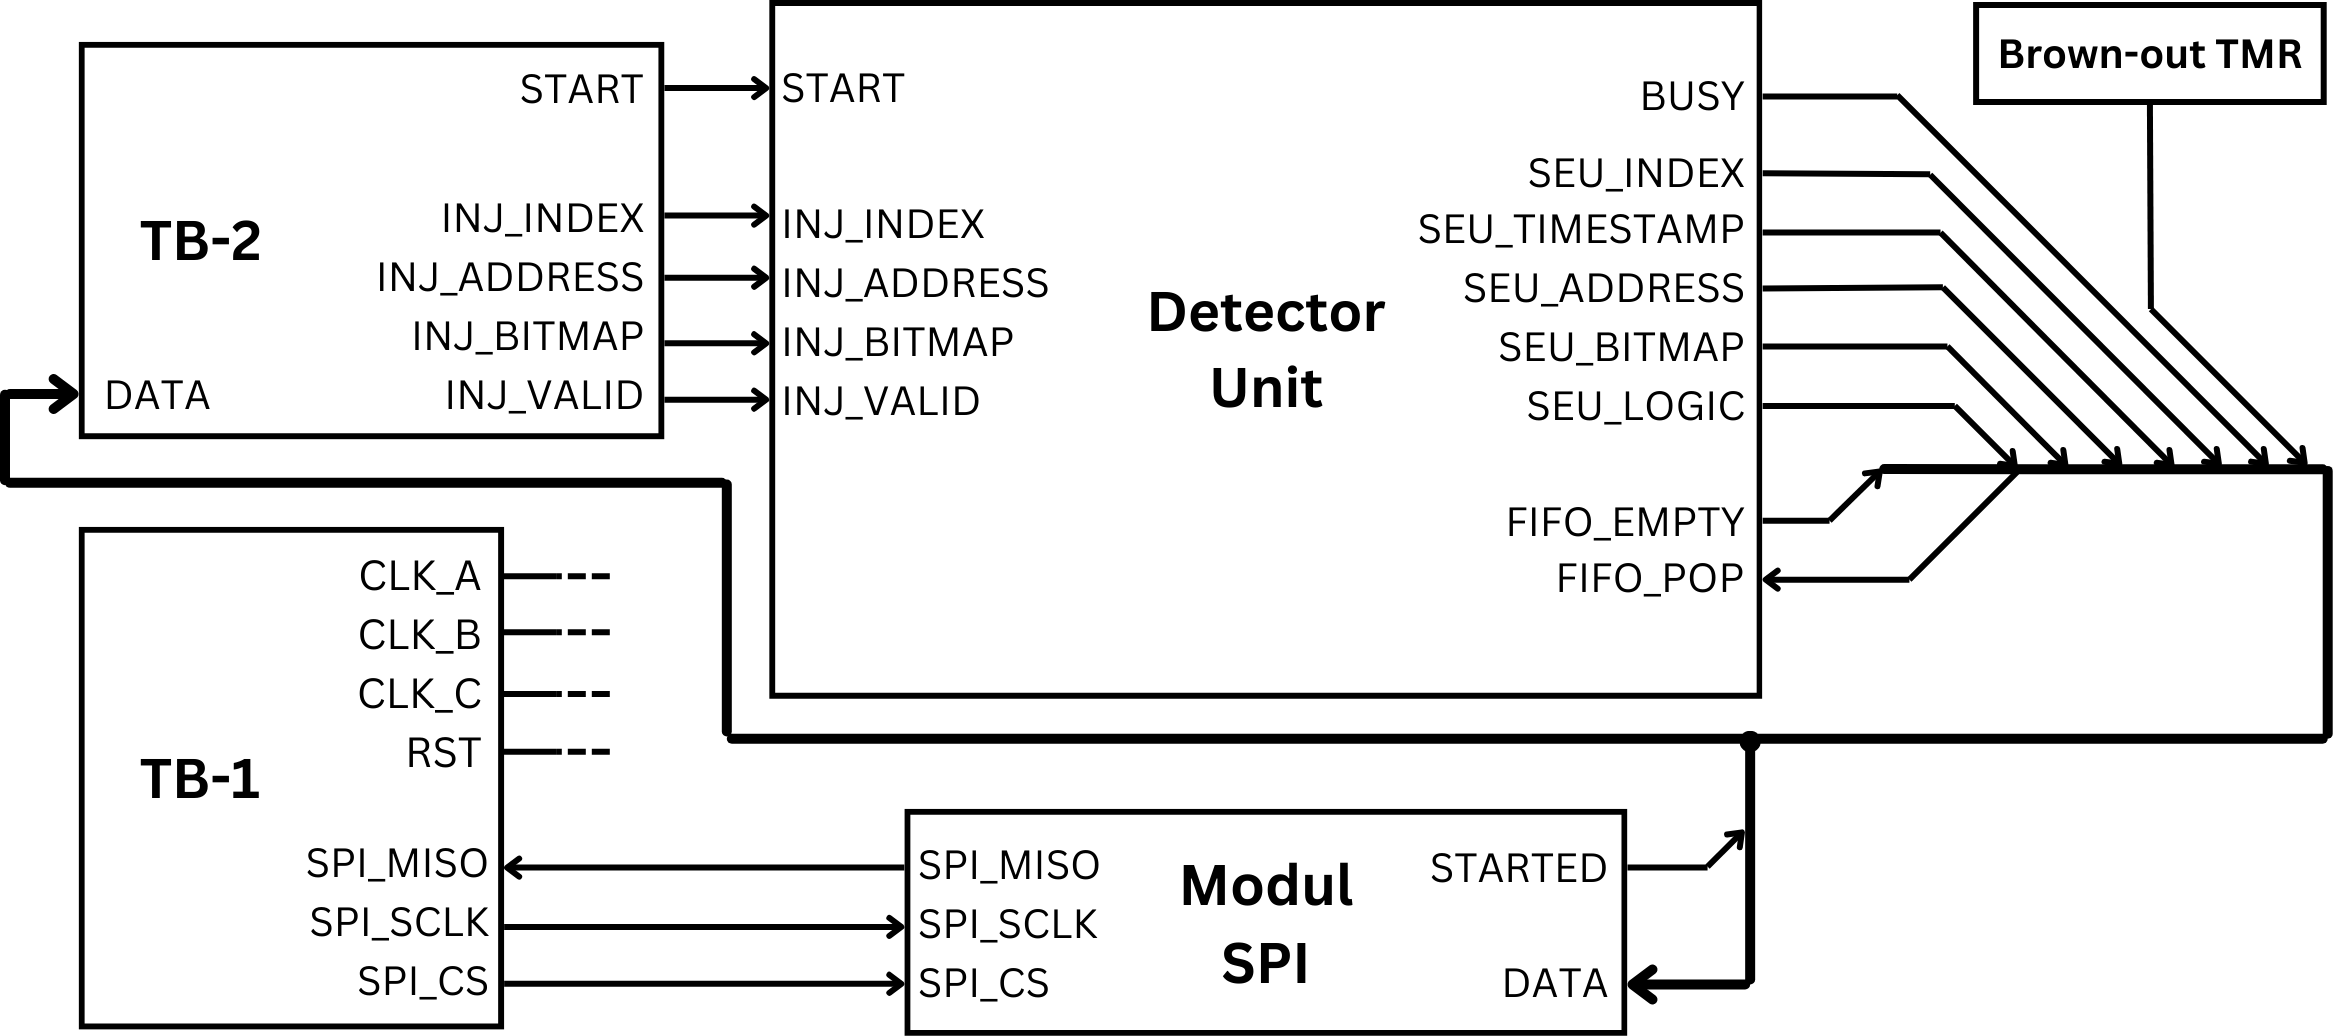
\includegraphics[width=\columnwidth]{./Images/ts_simulation_diagram.png}
    \caption{Schema bloc a testbench-urilor pentru simularea modulului Top.}%
    \label{fig:ts_simulation_diagram}
\end{figure}

Rezultatul simulării este prezentat în Figura \ref{fig:ts_main_sim} și este conform cu comportamentul așteptat ilustrat în Figura \ref{fig:sw_de_waveforms}. De sus în jos, se poate observa unul dintre cele trei semnale de ceas de 10 MHz, urmat de interfața de injectare a erorilor, prin intermediul căreia sunt inserate patru erori cu ajutorul celui de-al doilea \gls{tb}. Se remarcă faptul că două dintre erorile inserate au aceeași adresă de memorie, dar aparțin unor blocuri diferite. În această situație, eroarea asociată blocului cu index mai mare este ignorată în procesul de stocare a erorilor, aspect confirmat la finalul simulării, unde sunt detectate doar trei din cele patru erori 

În continuare, sunt prezentate semnalele corespunzătoare modulului \gls{de} care conține memoria cu indexul 3. După o perioadă de așteptare, este pornit procesul de scanare a memoriilor, permițând incrementarea contoarelor de adresă și evaluarea valorilor stocate de către logica de detecție. La trei tacte de ceas după selectarea adresei 9, este detectată o valoare eronată în memorie, corespunzătoare biților 0 și 2. Această eroare este raportată către \gls{du} și este corectată intern prin utilizarea celui de-al doilea port al memoriei.

\begin{figure}[ht!]
    \centering
    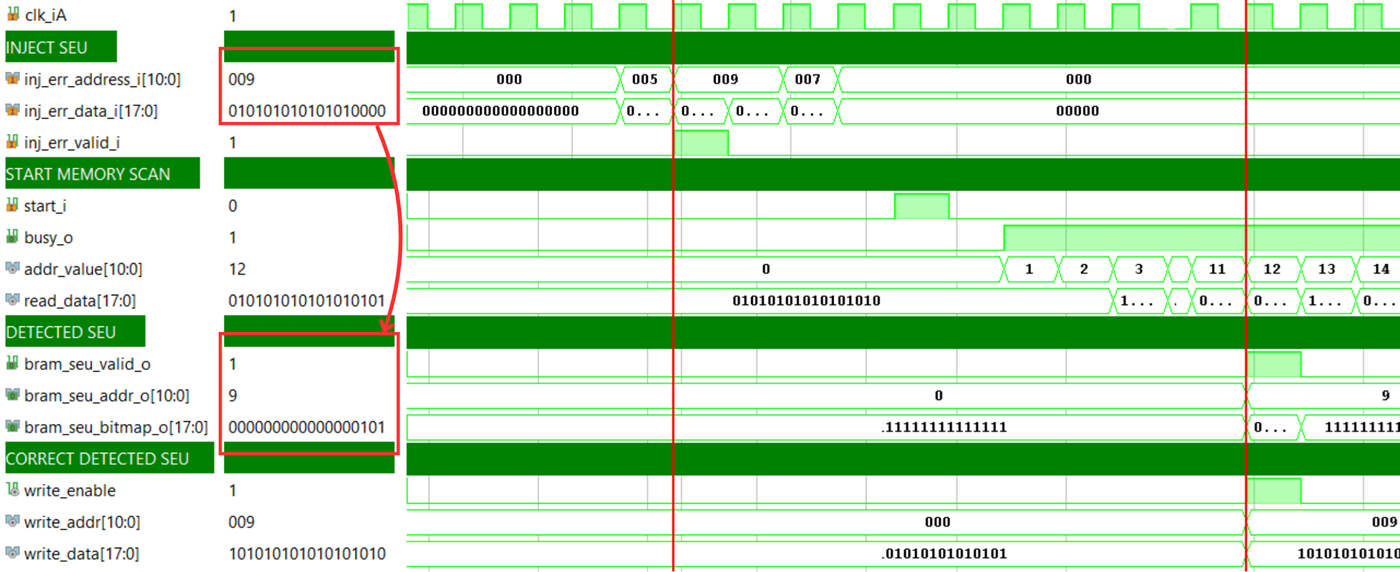
\includegraphics[width=\columnwidth]{./Images/ts_main_sim.png}
    \caption{Simularea modulului Top: inserarea, detectarea și corectarea erorilor SEU.}
    \label{fig:ts_main_sim}
\end{figure}

Odată ce simulările au produs rezultatele așteptate și toate defectele au fost corectate, s-a trecut la etapa de sintetizare și implementare a configurării, urmată de testarea fizică a sistemului. Metoda principală de testare a constat în utilizarea \gls{ip}-ului \gls{vio}, care a fost inserat în locul celui de-al doilea \gls{tb}, având aceleași intrări și ieșiri. Acest lucru a fost realizat prin utilizarea directivelor \textit{`ifdef SYNTHESIS -- `else -- `endif }, care permit includerea selectivă a unor secțiuni de cod doar în procesul de sinteză, în timp ce pentru simulare este utilizată cealaltă ramura a structurii. 

Prin alimentarea plăcii și conectarea \gls{fpga}-ului la un calculator, prin cablul de programare \gls{jtag}, a fost posibilă inserarea și controlarea semnalelor în timp real, fie prin interfața grafică Vivado, fie prin comenzi \gls{tcl}. A fost urmată aceeași procedură de testare ca în simulare: inserarea mai multor erori la adrese și memorii diferite, pornirea manuală a unei scanări (timer-ul \gls{tmr} descris în Capitolul \ref{sw_general_structure}, care pornește automat scanările, fiind inhibat printr-un semnal din \gls{vio}) și monitorizarea \gls{fifo}-ului de ieșire. De asemenea, au fost verificate codurile checksum și de paritate, confirmându-se faptul că acestea sunt conforme cu datele care le-au generat. În plus, s-a validat funcționarea corectă a celorlalte semnale de status din modulul Top, precum semnalul de brown-out, numărătorul de scanări și timer-ul de start. 

O componentă care nu a putut fi testată este detecția erorilor de tip \gls{seu} logic, apărute în logica combinațională, deoarece nu există o metodă practică de a modifica controlat un singur \gls{ff} dintr-o ramură a unei structuri \gls{tmr}. De asemenea, testarea sistemului fără inserarea manuală de erori nu a fost posibilă din cauza lipsei unei surse de radiație controlată.

\subsection{Testarea modulului SEM}
Testarea modulului \acrfull{sem} nu poate fi realizată în mediul de simulare Vivado, din cauza lipsei modelelor comportamentale pentru acest \gls{ip} și deoarece o scanare completă a memoriei durează aproximativ 183 ms, iar corectarea unei erori poate ajunge până la 554 ms \cite{pg036}. Din acest motiv, validarea modulului a fost efectuată exclusiv pe implementarea fizică a proiectului, utilizând \gls{ip}-ul \gls{vio}. Pentru utilizarea modului \gls{sem}, prin interfața \gls{vio}, au fost expuse semnalele descrise în Capitolul \ref{sem}, respectiv semnalele \textit{status}, care indică starea curentă a mașinii de stări finite interne \gls{ip}-ului, interfața \textit{inject}, utilizată pentru controlul acestei mașini de stări, precum și alte semnale auxiliare necesare.

Obiectivele testării au fost verificarea faptului că modulul se inițializează și intră în starea de observare, precum și confirmarea comportamentului său în urma inserării unor erori. Mai exact, sa urmărit că modulul să detecteze erorile, să le clasifice în una dintre cele două categorii (esențiale sau non-esențiale) și să încerce corectarea acestora. Dacă corectarea erorii nu este posibilă, semnalul \textit{uncorrectable} trebuie să fie asertat, iar \gls{ip}-ul să oprească procesul de scanare și să intre în starea \textit{idle}. La detectarea fiecărei erori, contorul intern trebuie incrementat, iar după fiecare eroare necorectabilă, modulul este forțat înapoi în starea de scanare printr-o comanda hard-codată.

Comenzile folosite pentru testarea acestor funcționalități sunt prezentate în Tabelul \ref{tab:ts_sem_commands_list}, împreună cu ordinea aplicării, efectul acestora și eventuale observații. Semnalul \textit{inject\_address} de 40 de biți, poate fi împărțit în mai multe câmpuri cu funcționalități diferite, în funcție de comanda utilizată \cite{pg036}. De la cel mai semnificativ la cel mai puțin semnificativ bit, structura acestuia este următoarea:
\begin{itemize}
    \item Primii 4 biți selectează tranziția către o stare diferită sau o reinițializare sau resetare.
    \item Următorii 4 biți sunt setați la zero pentru inserarea unei erori în spațiul de adrese liniar (spre deosebire de spațiul fizic)
    \item 2 biți sunt utilizați pentru selectarea unui Super Logic Region (SLR). În cazul dispozitivului Artix-7 utilizat, există un singur SLR, astfel că această valoare rămâne zero.
    \item 17 biți în intervalul [0, 24088] selectează adresa cadrului.
    \item 7 biți în intervalul [0, 100] selectează cuvântului.
    \item 5 biți selectează bitul din cadrul cuvântului.
\end{itemize}

Au fost întâmpinate dificultăți la inserarea unor erori relevante, deoarece nu a fost găsită o metodă practică de a determina adresele din memoria de configurare care contribuie activ la implementarea proiectului (adrese esențiale), respectiv adrese în care inserarea unei erori ar conduce la erori necorectabile. Astfel, erorile au fost inserate la întâmplare, majoritatea acestora afectând zone non-esențiale ale memoriei, caz în care sunt ignorate de modulul \gls{sem} și nu vor fi corectate.

\begin{table}[ht]
    \footnotesize
    \centering
    \renewcommand{\arraystretch}{1.6} 
    \caption{Lista de comenzi pentru controlul modulului SEM folosind interfața inject.}%
    \label{tab:ts_sem_commands_list}
    \begin{tabular}{C{1cm} L{4cm} C{2.3cm} C{3.3cm} L{4cm}}
		\toprule
			\textbf{Nr.} & 
            \textbf{Comandă} & 
            \textbf{inject\_address [39:36]} & 
            \textbf{inject\_address [36:0]} & 
            \textbf{Observații}\\
		\midrule
            1 & Inițializare sistem (Reset global) 
              & 1011 
              & don't care 
              & Resetare și inițializare completă \\
            2 & Intrare în starea de observare 
              & 1010 
              & don't care 
              & Stare implicită după inițializare \\
            3 & Tranziție în starea idle 
              & 1110 
              & don't care 
              & Așteaptă comenzi externe \\
            4 & Injectarea unei erori controlate 
              & 1101 
              & \{regiune logică, cadru, cuvânt, bit\} 
              & Permisă exclusiv din starea idle \\
            \bottomrule
    \end{tabular}
\end{table}

\subsection{Testarea modulului SPI și a celorlalte interfețe de comunicație}
Interfața \gls{spi} este principala metodă de comunicație cu \gls{obc}-ul și, în consecință, a necesitat o atenție sporită în procesul de testare. Primul pas a fost simularea modulului \gls{spi} în Vivado, unde au fost validate caracteristicile de fază și polaritate pentru fiecare dintre cele patru moduri \gls{spi}, precum și inițierea și terminarea corectă a tranzacțiilor în funcție de semnalul \gls{cs}. De asemenea, s-a verificat alinierea corectă a datelor, precum și încărcarea și golirea registrelor interne. Simularea începutului unei tranzacții \gls{spi} este prezentată în Figura \ref{fig:ts_spi_sim}, unde se observă încărcarea registrului de date, incrementarea \gls{fifo}-ului utilizat pentru stocarea erorilor și temporizarea tranzacției, prin captarea semnalului \gls{cs} cu o întârziere de o perioadă de ceas. De asemenea, schimbarea datelor are loc pe frontul descrescător al semnalului de ceas, conform modului 0 de funcționare.

\begin{figure}[ht!]
    \centering
    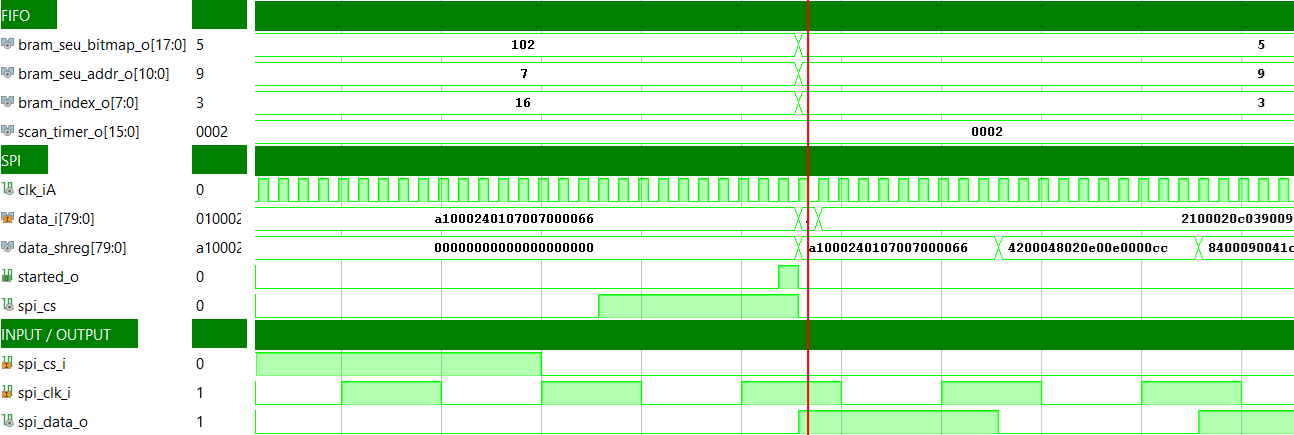
\includegraphics[width=\columnwidth]{./Images/ts_spi_sim.png}
    \caption{Simularea interfeței SPI: inițierea tranzacției și temporizarea semnalelor.}
    \label{fig:ts_spi_sim}
\end{figure}

Al doilea set de teste a constat în realizarea comunicațiilor fizice între \gls{fpga} și alte dispozitive. Un pachet de test a fost transmis cu succes către o placă Arduino Due, rezultatul fiind observat în Figura \ref{fig:sw_spi_waveforms_real}. Au fost testate diferite secvențe de date atât între \gls{fpga} și placa Arduino Due, cât și cu două plăci ESP32 și cu placa \gls{obc}. În plus, au fost transmise pachete de date în formatul final, verificându-se transformarea corectă a șirului de 80 biți în valorile corespunzătoare registrului de status, coordonatele erorilor detectate și codurile de detecție a erorilor de tip \gls{seu}.

Au fost validate atât semnalele single-ended, cât și semnalele diferențiale principale. În cazul testelor efectuate cu \gls{obc}-ul nanosatelitului, liniile au fost conectate direct prin conectorul PC-104 la driverul \gls{lvds} de pe placa master. Pentru testele cu ESP32, a fost utilizat un modul transceiver \gls{lvds} intermediar între placa \gls{aicors} și ESP32. Acest modul se bazează pe cipul SN65LVDT41 de la Texas Instruments, același circuit utilizat și pe \gls{obc}, asigurând astfel compatibilitatea electrică și funcțională.

În final, s-a confirmat că modulul \gls{spi} proiectat este stabil și funcționează corect la frecvența de 1 MHz. Această limitare de frecvența provine din arhitectura modulului, care utilizează trei bistabile de întârziere pentru implementarea un filtru de zgomot. Acest filtru introduce o latență suplimentară în reacția modulului la fronturile semnalului de ceas, reducând frecvența maximă de operare. În Figura \ref{fig:ts_spi_diff_frame} este ilustrat începutul unei tranzacții \gls{lvds} \gls{spi} la frecvența de 1.6 MHz. Se poate observa transmiterea corectă a datelor, semnalele de pe liniile diferențiale \gls{mosi} având un interval suficient pentru stabilirea valorii înaintea următorului tact de ceas. Din aceeași figură se pot observa nivelele corecte ale interfeței \gls{lvds} și forme de undă curate, cu distorsiuni minime, mult sub pragul la care ar putea apărea erori de comunicație.

\begin{figure}[ht!]
    \centering
    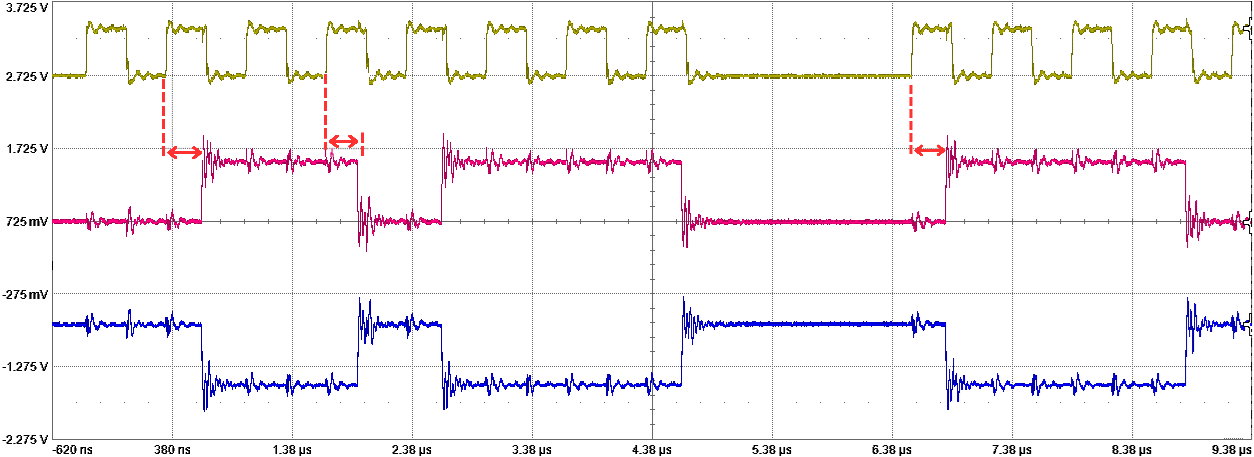
\includegraphics[width=\columnwidth]{./Images/ts_spi_diff_frame.png}
    \caption{Formele de undă reprezentând începutul unei tranzacții LVDS SPI.}%
    \label{fig:ts_spi_diff_frame}
\end{figure}

Pentru interfața auxiliară \gls{i2c}, utilizată pentru monitorizarea senzorilor de curent INA219 și cipului \gls{io} Expander, au fost efectuate aceleași tipuri de teste descrise anterior. Accentul a fost pus însă pe comunicarea cipurilor auxiliare cu \gls{obc}-ul, și nu cu \gls{fpga}-ul, datorită alegerilor făcute privind structura generală a proiectului. În acest scop, testarea a fost făcuta pe trei platforme diferite: Arduino, ESP32 și \gls{obc}, fiind verificate toate funcționalitățile disponibile ale cipurilor. Pentru senzorii de curent, au fost configurați regiștrii interni și au fost citite valorile de curent, tensiune și putere consumată. În cazul cipului \gls{io} Expander, au fost citite toate liniile de intrare pentru a confirma corectitudinea datelor, iar semnalele de ieșire au fost scrise și verificate, fie prin citirea lor de către \gls{fpga}, fie prin măsurarea directă cu osciloscopul, pentru a confirma asertarea corectă.

\section{Testarea hardware a PCB-ului}
După proiectarea, asamblarea și livrarea primei versiuni a plăcii \gls{aicors}, au fost începute procesele de testare și validare funcțională și electrică, cu scopul de a identifica problemele apărute în etapele de proiectare și fabricație, pentru a putea fi corectate în versiunea a doua a \gls{pcb}-ului. După o perioadă suficientă de testare, în urma căreia s-a considerat că toate problemele esențiale, la nivel de hardware și interfață, au fost identificate, a fost proiectată și comandată a doua versiune a plăcii, care a trecut cu succes prin aceeași suită de teste. Această versiune finală a fost testată suplimentar în combinație cu \gls{obc}-ul nanosatelitului, asigurându-se compatibilitatea completă între cele două sisteme.

Toate testele descrise în această secțiune pot fi considerate valide pentru ambele versiuni ale \gls{pcb}-ului, cu anumite excepții care vor fi menționate acolo unde este cazul. Instrumentele folosite pentru testare includ: un osciloscop HDO9404-MS de la Teledyne Lecroy \cite{oscilloscope_lecroy}, un osciloscop ADP2230 de la Digilent \cite{oscilloscope_digilent}, un dispozitiv de măsurare a consumului FNB58 de la FNIRSI \cite{usb_power_meter}, o cameră termală Flir One Edge \cite{thermal_camera}, o sursă de tensiune, un multimetru digital, precum și diverse plăci de dezvoltare Arduino și ESP32.

% \subsection{Testarea funcționalităților de bază ale PCB-ului}
Funcționalitățile de bază includ toate testele care pot fi efectuate fără alimentarea plăcii, inspecțiile vizuale, măsurătorile pentru verificarea dimensiunilor mecanice, precum și testele de alimentare stabilă și funcționarea corectă a \gls{fpga}-ului. Acestea cuprind verificarea alimentării și configurării \gls{fpga}-ului, integritatea liniilor \gls{gpio} și detectarea eventualelor scurt-circuite sau traseelor neconectate. Cele mai importante teste din această categorie sunt prezentate în Tabelul \ref{tab:ts_pcb_tests}, unde sunt enumerate denumirea fiecărui test și rezultatul obținut.

\begin{table}[h]
    \footnotesize
    \centering
    \renewcommand{\arraystretch}{1.6}
    \caption{Lista de teste efectuate pentru validarea de bază a PCB-ului AICoRS.}%
    \label{tab:ts_pcb_tests}
    \begin{tabular}{C{1cm} L{7.7cm} L{7cm}}
		\toprule
			\textbf{Nr.} & 
            \textbf{Test executat} & 
            \textbf{Rezultat}\\
		\midrule
            1 & Verificarea dimensiunilor mecanice ale \gls{pcb}-ului 
              & Dimensiuni conforme, abateri sub $\pm$0.1 mm \\
            2 & Verificarea grosimii \gls{pcb}-ului și a înălțimii maxime a ansamblului 
              & Grosime \gls{pcb}: 1.6 mm; înălțime maximă: 5 mm (excluzând conectorii) \\
            3 & Verificarea masei totale a plăcii 
              & 59 g $\pm$ 1 g \\
            4 & Inspecția vizuală pentru reziduuri de fludor și defecte de asamblare 
              & Fără reziduuri sau defecte vizibile \\
            5 & Verificarea atașării corecte a tuturor componentelor 
              & Conform \\
            6 & Verificarea continuității traseelor și absența scurtcircuitelor 
              & Fără discontinuități sau scurtcircuite \\
            7 & Măsurarea liniilor de alimentare 
              & Valori nominale, abateri sub $\pm$1\% \\
            8 & Verificarea inițializării și configurării corecte a \gls{fpga}-ului 
              & Succes \\
		\bottomrule
    \end{tabular}
\end{table}

Pe lângă testele enumerate anterior, a fost verificată și integritatea funcționării \gls{fpga}-ului în cazul defectării uneia sau mai multor linii de alimentare, precum și în situațiile în care tensiunile nu apar în ordinea corectă. În cazul liniilor de 1 V și 3.3 V, \gls{fpga}-ul se dezactivează complet, acestea fiind esențiale atât pentru logica internă, cât și pentru logica Blocului 0, responsabil cu controlul dispozitivului. Dacă tensiunea de 1.8 V dispare, \gls{fpga}-ul intră într-o stare nedeterminată, LED-urile de status luminând slab, însă dispozitivul se resetează și revine la o funcționare normală odată cu revenirea tensiunii. Pentru tensiunea de 2.5 V, \gls{fpga}-ul continuă să funcționeze corect, cu excepția comunicației prin interfața \gls{lvds}, driverele nefiind alimentate. Schimbarea ordinii de apariție a tensiunilor nu a avut un impact semnificativ asupra sistemului, iar în toate cazurile testate \gls{fpga}-ul nu a avut probleme permanente care să afecteze funcționarea ulterioară.

Au fost identificate două probleme în circuitul de alimentare al primei versiuni a \gls{pcb}-ului. Prima problemă a fost legată de rutarea liniilor de SENSE+ ale regulatoarelor de tensiune. Regulatoarele au fost proiectate astfel încât, prin intermediul unor jumpere, să poată fi deconectate de la liniile principale de alimentare ale \gls{pcb}-ului, permițând testarea lor independentă fără riscul deteriorării altor componente importante. Liniile de SENSE+ nu au avut însă un jumper dedicat, fiind conectate direct cât mai aproape de \gls{fpga}. În această configurație, atunci când regulatoarele sunt deconectate de la liniile de alimentare, pinii SENSE+ nu mai măsoară o tensiune corectă, ceea ce împiedică funcționarea corectă a regulatoarelor. Această problemă a fost remediată în versiunea a doua a \gls{pcb}-ului prin introducerea unui jumper dedicat pentru fiecare linie SENSE+.

A doua problemă a constat în instabilitatea regulatoarelor de tensiune cauzată de zgomot electric pe liniile de intrare. Fenomenul a fost produs de interacțiunea dintre mărgelele de ferită de pe intrare și condensatoarele de filtrare, care împreună formează un circuit rezonant LC slab amortizat. Acest efect, combinat cu caracteristica de impedanța negativă la intrare, specifică regulatoarelor în comutație, a condus la apariția unor oscilații care perturbau funcționarea acestora. Un exemplu al acestui fenomen este ilustrat în Figura \ref{fig:ts_ferrite_osc}, unde se observă creșterea amplitudinii oscilațiilor până la scăderea tensiunii sub 3 V, moment în care regulatorul se dezactivează și așteaptă reapariția unei tensiuni de intrare valide. Soluția adoptată a fost eliminarea mărgelelor de ferită, eliminând astfel componenta inductivă din circuit și stabilizând funcționarea regulatoarelor.

\begin{figure}[ht!]
    \centering
    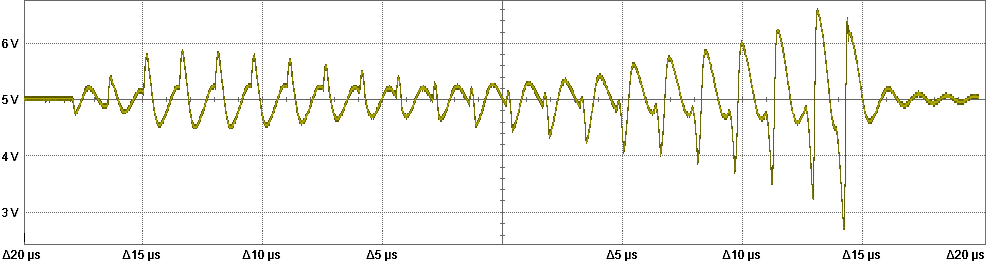
\includegraphics[width=\columnwidth]{./Images/ts_ferrite_osc.png}
    \caption{Oscilație de tensiune cauzată de mărgea de ferită și condensatoare de intrare.}
    \label{fig:ts_ferrite_osc}
\end{figure}

\subsection{Validarea integrității semnalelor și a alimentării}
Pentru evaluarea robusteții plăcii \gls{aicors} la zgomotul electromagnetic, cunoscut ca fiind mai intens în mediul spațial și o potențială sursă de degradare a performanței \cite{esa_radiation_space}, precum și pentru verificarea integrității generale a semnalelor, au fost măsurate diverse caracteristici ale liniilor \gls{gpio} și ale liniilor de alimentare. Analiza s-a concentrat în special asupra stabilității liniilor de alimentare la pornire și în regim de funcționare, fluctuațiilor semnalelor \gls{gpio}, fenomene de diafonie, supratensiuni și subtensiuni tranzitorii (overshoot și undershoot), precum și asupra timpilor de creștere și scădere ai semnalelor. În continuare sunt prezentate și discutate câteva dintre testele considerate cele mai relevante.

În Figura \ref{fig:ts_power_spikes} este ilustrat comportamentul liniei de alimentare de 5 V la pornirea \gls{pcb}-ului. Semnalul de sus reprezintă tensiunea la intrarea circuitului, semnalul din mijloc corespunde căderii de tensiune pe un rezistor de aproximativ 0.05 \(\Omega\) conectat în serie cu linia de alimentare, permițând astfel determinarea curentului de intrare, iar semnalul de jos reprezintă o mărire a primelor vârfuri observate în semnalul de curent.

La momentul alimentării \gls{pcb}-ului se observă un curent de pornire de aproximativ 2 A, cu o durată de circa 30 ms, asociat încărcării condensatorilor de intrare ai regulatoarelor de tensiune. După o perioadă configurabilă între 0 și 80 ms, determinată de funcția de soft-start a regulatoarelor, apar mai multe impulsuri scurte de curent, fiecare având o durată mai mică de 700 ns. Acestea corespund inițierea activității de comutație a regulatoarelor și sunt prezente până la stabilizarea buclei de reglaj. 

\begin{figure}[ht!]
    \centering
    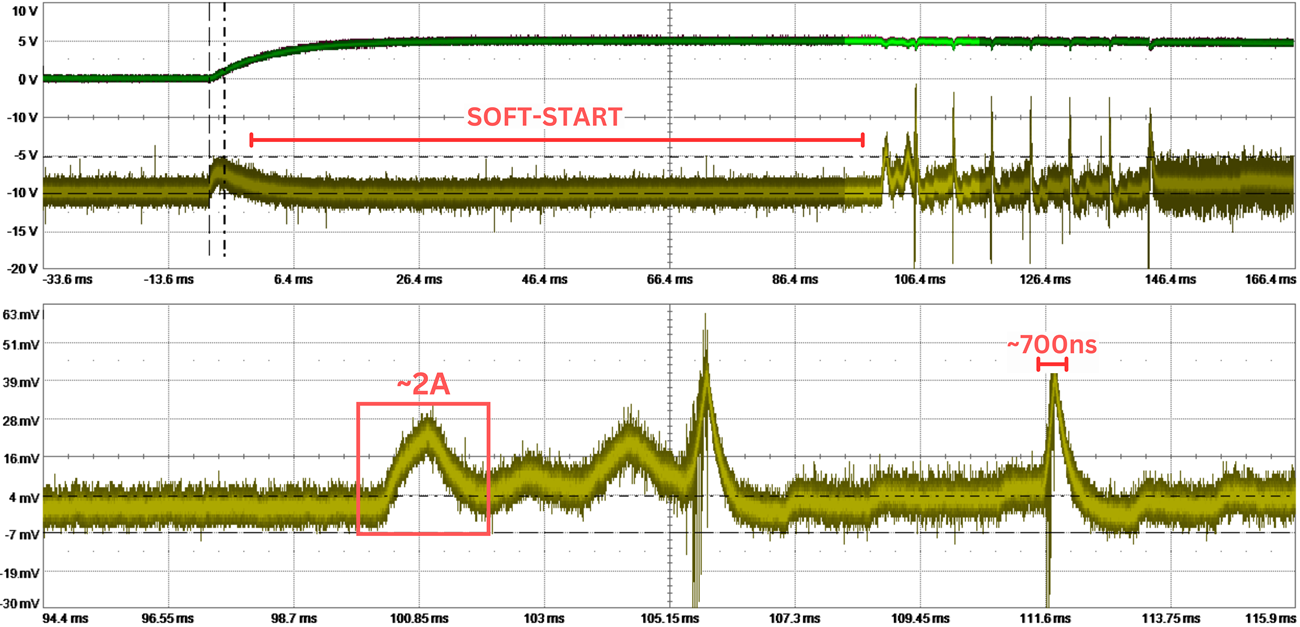
\includegraphics[width=\columnwidth]{./Images/ts_power_spikes.png}
    \caption{Vârfuri de curent observate la alimentarea plăcii AICoRS.}%
    \label{fig:ts_power_spikes}
\end{figure}

Deși acest comportament tranzitoriu este unul așteptat la pornirea unor regulatoare în comutație, primul vârf de curent, asociat încărcării condensatorilor de intrare, este suficient de mare pentru a declanșa controller-ul de supracurent de pe \gls{obc}-ul nanosatelitului, care întrerupe alimentarea plăcii. Soluțiile principale identificate pentru remedierea acestei probleme sunt fie reducerea capacității totale de pe linia de intrare de 5 V a \gls{pcb}-ului \gls{aicors}, prin îndepărtarea unei părți din condensatorii de filtrare, fie creșterea limitei superioare de curent acceptată sau implementarea unui mecanism de ignorare temporară a vârfului de curent de pornire la nivelul cipului controller.

În regim de funcționare stabil însă, regulatoarele operează în parametrii optimi. Integritatea alimentării a fost evaluată utilizând parametrii statistici furnizați de osciloscop, care au fost comparați cu limitele admise specificate în datasheet-ul \gls{fpga}-ului \cite{ds181}. Au fost analizate următoarele criterii:
\begin{itemize}
    \item Secvența de alimentare: liniile de 1 V, 1.8 V, 2.5 V și 3.3 V pornesc în ordinea corectă. Toate regulatoarele prezintă rampe de pornire mai mici de 1 ms, iar întârzierea dintre două regulatoare consecutive este mai mare de 1.5 ms, respectând secvența recomandată de Xilinx.
    \item Deviația în curent continuu (DC deviation): definită ca diferența dintre tensiunea nominală și cea măsurată. Pentru toate nivelurile de alimentare, deviația s-a menținut sub \(\pm 1\%\), inclusiv sub sarcină, indicând o reglare corespunzătoare și o distribuție stabilă a tensiunilor.
    \item Ondulație vârf-la-vârf (peak-to-peak ripple): reprezintă variația maximă a tensiunii. Acestea a fost sub 50 mV pentru linia de 1 V și sub 60 mV pentru celelalte linii de alimentare. Valorile se află sub limitele recomandate de 100 mV pentru linia de 1 V și 400 mV pentru restul.
    \item Valorile maxime și minime (overshoot, undershoot): măsurătorile indică faptul că valorile extreme sunt aproximativ egale cu jumătate din ondulația vârf-la-vârf, confirmând lipsa unor asimetrii semnificative sau a unor deplasări DC nedorite.
    \item Zgomotul \gls{rms}: reprezintă o măsură a energiei medii a variațiilor de zgomot din jurul tensiunii nominale. Aceasta a fost determinată din deviația standard a semnalului măsurat în cuplare AC și a avut valori sub 5.4 mV chiar și în condiții de sarcină, indicând un nivel redus al zgomotului pe liniile de alimentare.
    \item Analiză spectrală: pentru linia de 1 V aflată sub sarcină a evidențiat un nivel de zgomot de aproximativ -65 dBm (raportat la o impedanță de 50 \(\Omega\)), cu vârfuri izolate la 100, 200 și 300 MHz, corespunzătoare armonicilor generate de comutația logicii digitale, și la 630 MHz, frecvența de comutație a regulatorului. Toate aceste componente se află sub -38 dBm. Rezultatele confirmă un nivel scăzut de zgomot, iar topologia de decuplare utilizată (0,47 \(\mu\)F, 4,7 \(\mu\)F și 47 \(\mu\)F) asigură filtrarea corespunzătoare pe o bandă largă de frecvență.
\end{itemize}

Pentru generatorul principal de ceas de 100 MHz a fost parcurs un set similar de măsurători, cu scopul de a valida funcționarea corectă și stabilitatea semnalului furnizat \gls{fpga}-ului. Frecvența măsurată a fost de 100 MHz cu variații de 254 kHz, valoare aflată sub limitele recomandate. Jitter-ul ciclu-la-ciclu, definit ca diferența de timp dintre două perioade consecutive de ceas, s-a situat sub 42 ps. Factorul de umplere a fost de aproximativ 49.8 \%, iar timpii de creștere și descreștere au fost sub 2 ns. Nivelurile de tensiune sunt conforme cu standardul \gls{lvds}, iar timpul de la alimentarea plăcii până la funcționarea stabilă a generatorului de ceas a fost de 2.5 ms, confirmând funcționarea corectă și robustă a sursei de ceas.

Pentru semnalele \gls{gpio} provenite de \gls{fpga}, atât pe liniile \gls{lvds} \gls{spi}, cât și pe liniile \gls{i2c} și celelalte linii auxiliare, s-au determinat caracteristicile semnalelor și performața ansamblului din punctul de vedere al integrității semnalelor. Deși aceste teste depășesc cerințele actuale ale proiectului, liniile \gls{lvds} fiind testate la 250 MHz, în timp ce interfața \gls{spi} funcționează la 1 MHz, evaluarea tuturor liniilor \gls{gpio}, inclusiv a celor neutilizate între conectorul PC-104 și \gls{fpga}, oferă o imagine completă asupra performanței \gls{pcb}-ului în cele mai rele condiții. Aceste informații sunt utile atât pentru îmbunătățiri viitoare ale plăcii, cât și pentru evaluarea eligibilității sale în proiecte cu cerințe mai intensive.

Pentru testarea caracteristicile liniilor, a fost implementat un proiect Verilog controlabil prin interfața \gls{vio}, care permite generarea semnalelor dreptunghiulare cu frecvențe variabile, derivate din semnalul de ceas principal. A fost inclusă o mască de ieșire pentru aplicarea semnalelor doar pe liniile dorite, precum și un generator \gls{lfsr} cu lungimea de 16 biți, pentru obținerea unei secvențe pseudo-aleatoare de biți, utilă în generarea diagramelor ochi.

\begin{itemize}
    \item Timpul de creștere și de scădere: Pentru semnalele cu standardul \gls{lvcmos33}, timpii de răspuns nu au depășit 770 ps, iar pentru semnalele \gls{lvds} nu s-a depășit 670 ps. Acești timpi permit, teoretic, funcționarea la frecvențe de ordinul sutelor de MHz, limita practică fiind impusă de cerințele de temporizare și jitter-ul logicii digitale. În cazul interfeței \gls{i2c}, timpii de creștere sunt mult mai mari din cauză structurii protocolului și a rezistorilor de pull-up, capacității liniilor și driverelor cu drenă comună, ridicând timpul de răspuns la aproximativ 300 ns, suficient pentru modul rapid de 400 kHz al interfeței \gls{i2c}.
    \item Supratensiuni și subtensiuni tranzitorii (overshoot și undershoot): pe liniile \gls{lvcmos33}, au fost observate vârfuri de ±1 V cu durata de circa 2.5 ns, cauzate de fronturile rapide ale \gls{fpga}-ului și de lipsa terminării la capătul conectorului. Deși tensiunea depășește nivelul nominal cu 20\%, durata scurtă a acestora nu afectează funcționarea logică a sistemului.
    \item Semnalelor diferențiale \gls{lvds}: tensiunea de mod comun a rămas stabilă în jurul valorii nominale, iar variațiile tranzitorii observate pe liniile individuale (±100 mV) nu afectează semnalul diferențial și se încadrează în limitele specificațiilor.
    \item Cuplajul între liniile \gls{gpio} de 3.3 V: aplicând un semnal dreptunghiular pe un traseu, pe cel mai apropiat traseu (la distanța de 0.8 mm) s-au observat un vârf pozitiv de 200 mV, urmat de unul negativ de -100 mV, corespunzând cuplajului capacitiv și inductiv. Pentru un traseu mai îndepărtat, la distanța minimă între trasee de 2.8 mm, vârful s-a redus la 50 mV. Aceste valori maxime durează sub 1 ns și se situează mult sub nivelele logice, fără efect asupra funcționării sistemului.
\end{itemize}

În Figura \ref{fig:ts_eye_diagram} este prezentată o diagramă ochi realizată pe o pereche de linii din interfața \gls{lvds} \gls{spi}. Testul a fost efectuat prin transmiterea unui șir de biți pseudo-aleatorii la frecvența de 250 MHz, iar semnalul diferențial a fost măsurat la capătul conectorului PC-104. Se observa o deschidere largă a ochiului, ceea ce indică o marjă largă de zgomot și de temporizare. Ochiul este simetric, atât în tranziție dintre nivelele de tensiune, cât și în privința factorului de umplere și a nivelelor de tensiune.

Deschiderea verticală a ochiului variază între 0.7 V (minim) și 1.2 V (maxim), valori care se încadrează între limitele electrice specificate de documentația Xilinx. Lățimea este de 4 ns, diferența temporală a punctelor de tranziție fiind redusă, ceea ce asigură o marjă temporală suficientă pentru eșantionare precisă. Variația punctului de trecere prin zero (zero-crossing)  este sub 400 ps, indicând un jitter scăzut și o sincronizare stabilă a liniilor diferențiale. 

\begin{figure}[ht!]
    \centering
    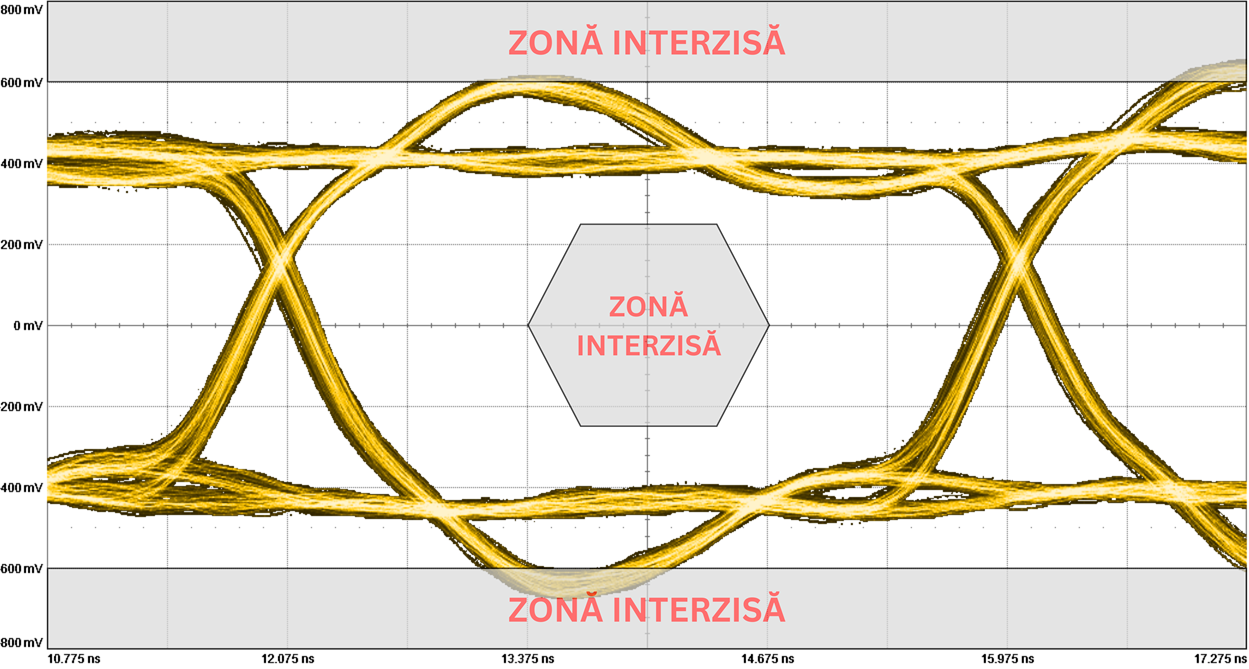
\includegraphics[width=\columnwidth]{./Images/ts_eye_diagram.png}
    \caption{Diagrama ochi efectuată pe o linie a interfeței LVDS SPI la 250 Mhz.}%
    \label{fig:ts_eye_diagram}
\end{figure}

Diagrama de ochi prezintă o ușoară distorsiune în apropierea punctului de decizie, manifestată prin vârfuri de tensiune de până la \(\pm\)600 mV. Aceste variații sunt cauzate de limitările de bandă și de efectele inter-simbol la frecvența de test de 250 MHz. Cu toate acestea, punctul de trecere prin zero rămâne clar definit, iar amplitudinea semnalului se menține în limitele specificației \gls{lvds}.

\subsection{Evaluarea consumului de energie}
Pentru evaluarea consumului de energie al \gls{fpga}-ului și al \gls{pcb}-ului \gls{aicors}, precum și pentru a verifica încadrarea acestuia în limitele acceptate de platforma nanosatelitului, au fost realizate mai multe simulări și măsurători pentru diferite configurații de funcționare. Testele au fost efectuate inițial pe prima versiune a \gls{pcb}-ului, cu scopul de a identifica eventuale modificări necesare pentru versiunea a doua a plăcii. După fabricarea celei de-a doua versiuni, măsurătorile au fost reluate pentru a confirma îmbunătățirile implementate.

Această evaluare a fost prezentată pentru prima dată în lucrarea "Power and Cross-Section Optimization for an \gls{fpga}-Based Cosmic Radiation Sensor", realizată în coautorat în 2025 \cite{icecs}. O parte dintre rezultatele și metodologiile prezentate în acest articol sunt preluate și detaliate în secțiunea următoare. 

Ideea generală a constat în implementarea mai multor variații ale configurației principale de detecție și corecție a evenimentelor \gls{seu}, urmate de măsurarea consumului de energie atât prin metode experimentale, cât și prin utilizarea uneltelor software de estimare a consumului integrate în mediul de dezvoltare Vivado. Principalii parametrii care au fost modificați în cadrul acestor experimente au fost:
\begin{itemize}
    \item Frecvența semnalului de ceas: 10 MHz, 25 MHz, 50 MHz și 100 MHz.
    \item Gradul de utilizare al blocurilor de memorie ale \gls{fpga}-ului: 25\%, 50\%, 75\% și 100\%.
    \item Frecvența de scanare a memoriilor: 12 Hz, 120 Hz, 1.2 kHz și 12 kHz. Aceste frecvențe au fost determinate în funcție de durata unei scanări complete a memoriei și de procentul de timp în care circuitul este activ. Frecvențele corespund unor factori de umplere de 0.1\%, 1\%, 10\% și 100\%. 
    \item Adăugarea unui microprocesor MicroBlaze pe lângă modulul de detecție.
    \item Utilizarea unor opțiuni speciale de sintetizare și implementare pentru modulele \gls{hdl}.
\end{itemize}

Prima metodă de estimare a consumului de energie a constat în simulări comportamentale și în utilizarea uneltei Vivado Power Analysis Tool din mediul de dezvoltare Vivado. Această unealtă ia în considerare parametrii precum activitatea de comutație a semnalelor, temperatura internă a dispozitivului, tensiunile nominale de alimentare și curenții de scurgere ai tranzistorilor. 

Pentru caracterizarea activității de comutație au fost utilizate două metode: atribuirea unor valori medii aplicate global și generarea unui fișier Switching Activity Interchange Format (SAIF) în timpul simulării comportamentale. Fișierul SAIF conține informații detaliate despre comportamentul fiecărui semnal, precum rata de comutație și probabilitatea statică (probabilitatea ca un semnal să se afle într-un nivel logic 0 sau 1). Aceste date pot fi mai târziu corelate cu semnalele reale din proiectul implementat, pentru a obține o estimare cât mai realistă a consumului. Pentru semnalele care nu au putut fi corelate, s-au utilizat valori standard de 70\% pentru rata de comutație și 0.5 pentru probabilitatea statică. Rata de comutație a fost crescută intenționat față de valoarea implicită de 12.5\%, pentru a reflecta comportamentul în timpul unei scanări, în care biții din logica de date comută la fiecare perioadă de ceas. 

În Figura \ref{fig:ts_power_measurements_setup} este prezentată configurația fizică a experimentului. \gls{pcb}-ul \gls{aicors} este conectat la un PC prin cablul de programare \gls{jtag} și este alimentat printr-un cablu Micro-\gls{usb}, la care este atașat dispozitivul FNB58 pentru măsurarea consumului de energie. În plus, cei patru senzori de curent INA219 comunică prin interfața \gls{i2c} cu un Arduino Uno Rev 3, care rulează un program de eșantionare la un interval prestabilit. Arduino-ul este conectat la conectorul PC-104 al \gls{pcb}-ului și la PC printr-un cablu \gls{usb}, permițând monitorizarea consumului în timp real.

\begin{figure}[ht!]
    \centering
    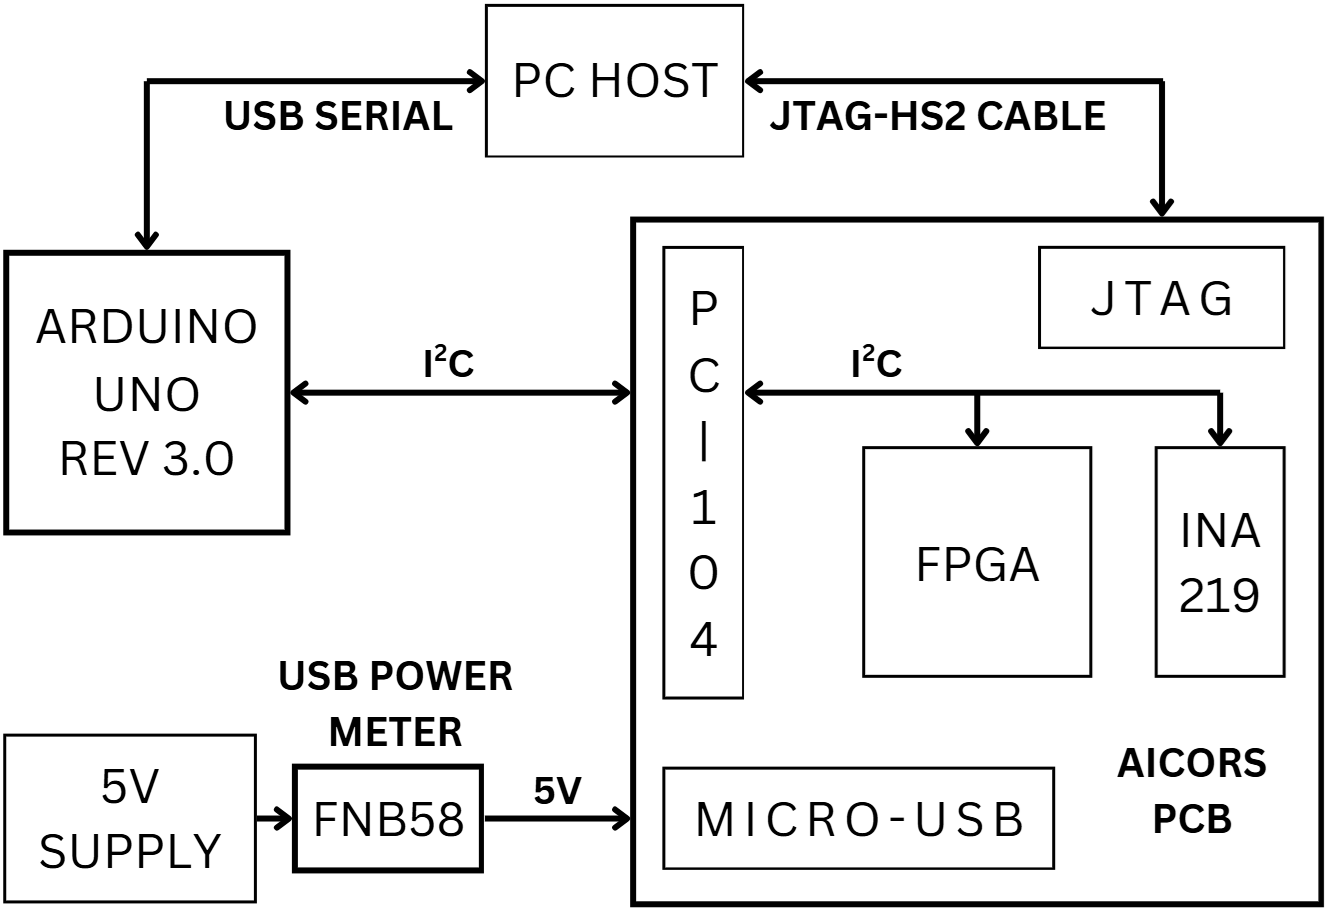
\includegraphics[width=0.6\columnwidth]{./Images/ts_power_measurements_setup.png}
    \caption{Configurația fizică pentru măsurătorile consumului de energie al FPGA-ului.}%
    \label{fig:ts_power_measurements_setup}
\end{figure}

Având în vedere că, în cazul măsurătorilor reale, intervin mai multe elemente decât dispozitivul \gls{fpga}, a fost necesară calibrarea valorilor obținute de la senzorii INA219 cu cele furnizate de unealta de estimare a consumului, pentru obține rezultate coerente. În Figura \ref{fig:ts_consumption_calibration} sunt prezentate măsurătorile și estimările corespunzătoare unei configurații minime a \gls{fpga}-ului. Aceasta constă în propagarea semnalului principal de 100 MHz către o ieșire \gls{gpio}, utilizând un număr redus de resurse logice, permițând astfel determinarea consumului de bază al \gls{fpga}-ului asociat exclusiv alimentării și programării acestuia.

Din figură se poate observa că valorile măsurate sunt apropiate de cele estimate, cu excepția liniei de 3.3 V, unde consumul real este de peste 10 ori mai mare, crescând de la 26 mW la 303 mW. Dacă acest consum suplimentar este exclus din calculul consumului total, conform ultimei valori prezentate în figură, rezultatele se aliniază cu o abatere de 10\%. 

În consecință, și având în vedere faptul ca \gls{fpga}-ul nu utilizează porturi \gls{gpio} alimentate la 3.3 V, se poate concluziona că diferența de 277 mW (303 mW minus 26 mW, corespunzătoare consumului blocului 0 al \gls{fpga}-ului) este atribuită altor componente ale \gls{pcb}-ul \gls{aicors}. Acest consum suplimentar provine în principal de la cipul de conversie \gls{usb} la \gls{uart}/\gls{jtag}, care are un consum static de aproximativ 70 mA conform datasheet-ului \cite{ft2232h_datasheet}, precum și de la generatorul de ceas (aproximativ 16 mA) și memoriei FLASH.

\begin{figure}[h]
    \centering
    \begin{tikzpicture}
        \begin{axis}[
            ybar,
            bar width=16pt,
            enlarge x limits=0.22,
            enlarge y limits=0.2,
            ylabel={Putere [mW]},
            symbolic x coords={1 V, 1.8 V, 3.3 V, Total},
            xtick=data,
            width=12cm,
            height=6cm,
            grid=major,
            nodes near coords,
            tick label style={font=\footnotesize},
            every node near coord/.append style={font=\footnotesize},
            legend style={at={(0.5,-0.2)}, anchor=north, legend columns=3, column sep=7pt}
        ]
        
        % First plot
        \addplot+[blue, fill=blue!20] coordinates {(1 V,  73)(1.8 V,  190)(3.3 V, 303)(Total, 566)};
        \addlegendentry{Măsurători [mW]}
        \addplot+[red, fill=red!20] coordinates {(1 V,  34)(1.8 V,  200)(3.3 V, 26)(Total, 260)};
        \addlegendentry{Estimări [mW]}
        \addplot+[brown, fill=brown!20] coordinates {(Total, 234)};
        \addlegendentry{Măsurători fără 3.3 V [mW]}
        
        \end{axis}
    \end{tikzpicture}
    \caption{Rezultatele măsurătorilor și a estimărilor consumului de energie al FPGA-ului.}%
\label{fig:ts_consumption_calibration}
\end{figure}

Măsurătorile efectuate cu monitorul \gls{usb} FNB58 corespund cu rezultatele prezentat anterior, indicând însă un consum suplimentar de aproximativ 1.25 W. Deși această valoare este de cinci ori mai mare decât consumul estimat, ea poate fi atribuită în mare parte celor șase LED-uri de status (125 mW x 6 = 750 mW), care au fost eliminate în a doua versiune a \gls{pcb}-ului, precum și pierderilor introduse de regulatoarele de tensiune. La niveluri scăzute de sarcină, regulatoarele de tensiune în comutație își reduc semnificativ eficiența, fenomen accentuat de configurația minimă a \gls{fpga}-ului și de lipsa consumului pe linia de 2.5 V, activă doar în timpul comunicației prin interfața \gls{lvds} \gls{spi}.

Pentru a simplifica procesul de testare și a reduce numărul de configurații \gls{hdl} necesare, caracteristicile analizate au fost grupate în trei evaluări principale: rata de utilizare a memoriei cu frecvența semnalului de ceas, adăugarea unui procesor MicroBlaze împreună cu opțiunile de optimizare a consumului, și frecvența de scanare a memoriilor. Dintre acestea, cei mai importanți factori sunt frecvența semnalului de ceas și numărul de blocuri de memorie utilizate. Rezultatele sunt prezentate în Figura \ref{fig:ts_freq_vs_utiliz}, unde valorile au fost obținute ca medie aritmetică între măsurătorile reale corectate și estimările software.

Se observă că atât frecvența semnalului de ceas, cât și gradul de utilizare a memoriei influențează consumul de energie într-un mod liniar. Totuși, frecvența principală are un impact mai mare: consumul crește de la 522 mW la 10 MHz la 3186 mW la 100 MHz. Creșterile succesive de frecvență duc la majorări ale consumului între 33\% și 58\%, în timp ce creșterea utilizării memoriei creează variații mai moderate, între 13\% și 18\%.

În plus, configurațiile care combină o frecvență ridicată cu un grad mare de utilizare a memoriei, generează nu doar un consum mare de energie, ci și probleme termale și de implementare. Uneltele Vivado de sinteză și implementare nu mai reușesc să îndeplinească constrângerile de temporizare fără activarea unor opțiuni suplimentare de optimizare. De asemenea, temperatura pachetului \gls{fpga} depășește 75°C după aproximativ două minute de funcționare, pornind de la o temperatură ambientală de 25°C, în lipsa unui radiator.

% % -------- PLOT --------
% \begin{figure}[h!]
%     \centering
%     \begin{tikzpicture}
%         \begin{axis}[
%             width=8cm,
%             height=5.5cm,
%             xlabel={Frecvența ceasului [MHz]},
%             ylabel={Putere consumată [mW]},
%             xmin=0, xmax=110,
%             ymin=0, ymax=3400,
%             xtick={10,25,50,100},
%             ytick={0,500,1000,1500,2000,2500,3000,3500},
%             grid=major,
%             legend style={at={(0.5,-0.3)},anchor=north,legend columns=5},
%             thick,
%             mark options={solid}
%         ]
        
%          % ---- dummy plot for "Util:" ----
%         \addplot[draw=none] coordinates {(0,0)}; % invisible dummy plot
%         \addlegendentry{Util:};
%         % 25% utilization
%         \addplot+[mark=o] coordinates {(10,314) (25,419) (50,590) (100,934)};
%         \addlegendentry{25\%};
%         % 50% utilization
%         \addplot+[mark=square] coordinates {(10,385) (25,593) (50,924) (100,1630)};
%         \addlegendentry{50\%};
%         % 75% utilization
%         \addplot+[mark=triangle] coordinates {(10,454) (25,753) (50,1267) (100,2359)};
%         \addlegendentry{75\%};
%         % 100% utilization
%         \addplot+[mark=diamond] coordinates {(10,522) (25,937) (50,1629) (100,3186)};
%         \addlegendentry{100\%};

%         \end{axis}
%     \end{tikzpicture}
%     \caption{Consumul FPGA-ului în funcție de frecvența proiectului și utilizarea memoriilor.}
%     \label{fig:ts_freq_vs_utiliz_plot}
% \end{figure}

% % -------- TABLE --------

% \begin{table}[h!]
%     \footnotesize
%     \centering
%     \renewcommand{\arraystretch}{1.8} 
%     \caption{Tabelul corespunzător consumului FPGA-ului în funcție de frecvență și utilizarea memoriilor.}
%     \label{tab:ts_freq_vs_utiliz_table}
%     \begin{tabular}{C{2cm}C{1cm}C{1cm}C{1cm}C{1cm}}
% 		\toprule
% 			\textbf{Util. \textbackslash   Frec. [MHz]} & 10 & 25 & 50 & 100 \\
% 		\midrule
% 		    25\%  & \cellcolor{green!30} 314  
%                 & \cellcolor{green!35} 419  
%                 & \cellcolor{yellow!50} 590  
%                 & \cellcolor{orange!50} 934 \\
                                
%     		50\%  & \cellcolor{green!40} 385  
%                 & \cellcolor{yellow!60} \textbf{593}  
%                 & \cellcolor{orange!60} 924  
%                 & \cellcolor{red!35} 1630 \\
                                
%     		75\%  & \cellcolor{yellow!50} 454  
%                 & \cellcolor{orange!55} 753  
%                 & \cellcolor{orange!70} 1267 
%                 & \cellcolor{red!45} 2359 \\
                                
%     		100\% & \cellcolor{yellow!60} 522  
%                 & \cellcolor{orange!60} 937  
%                 & \cellcolor{red!30} 1629 
%                 & \cellcolor{red!70} 3186 \\
% 		\bottomrule
%     \end{tabular}
% \end{table}

\begin{figure}[ht!]
    \centering
    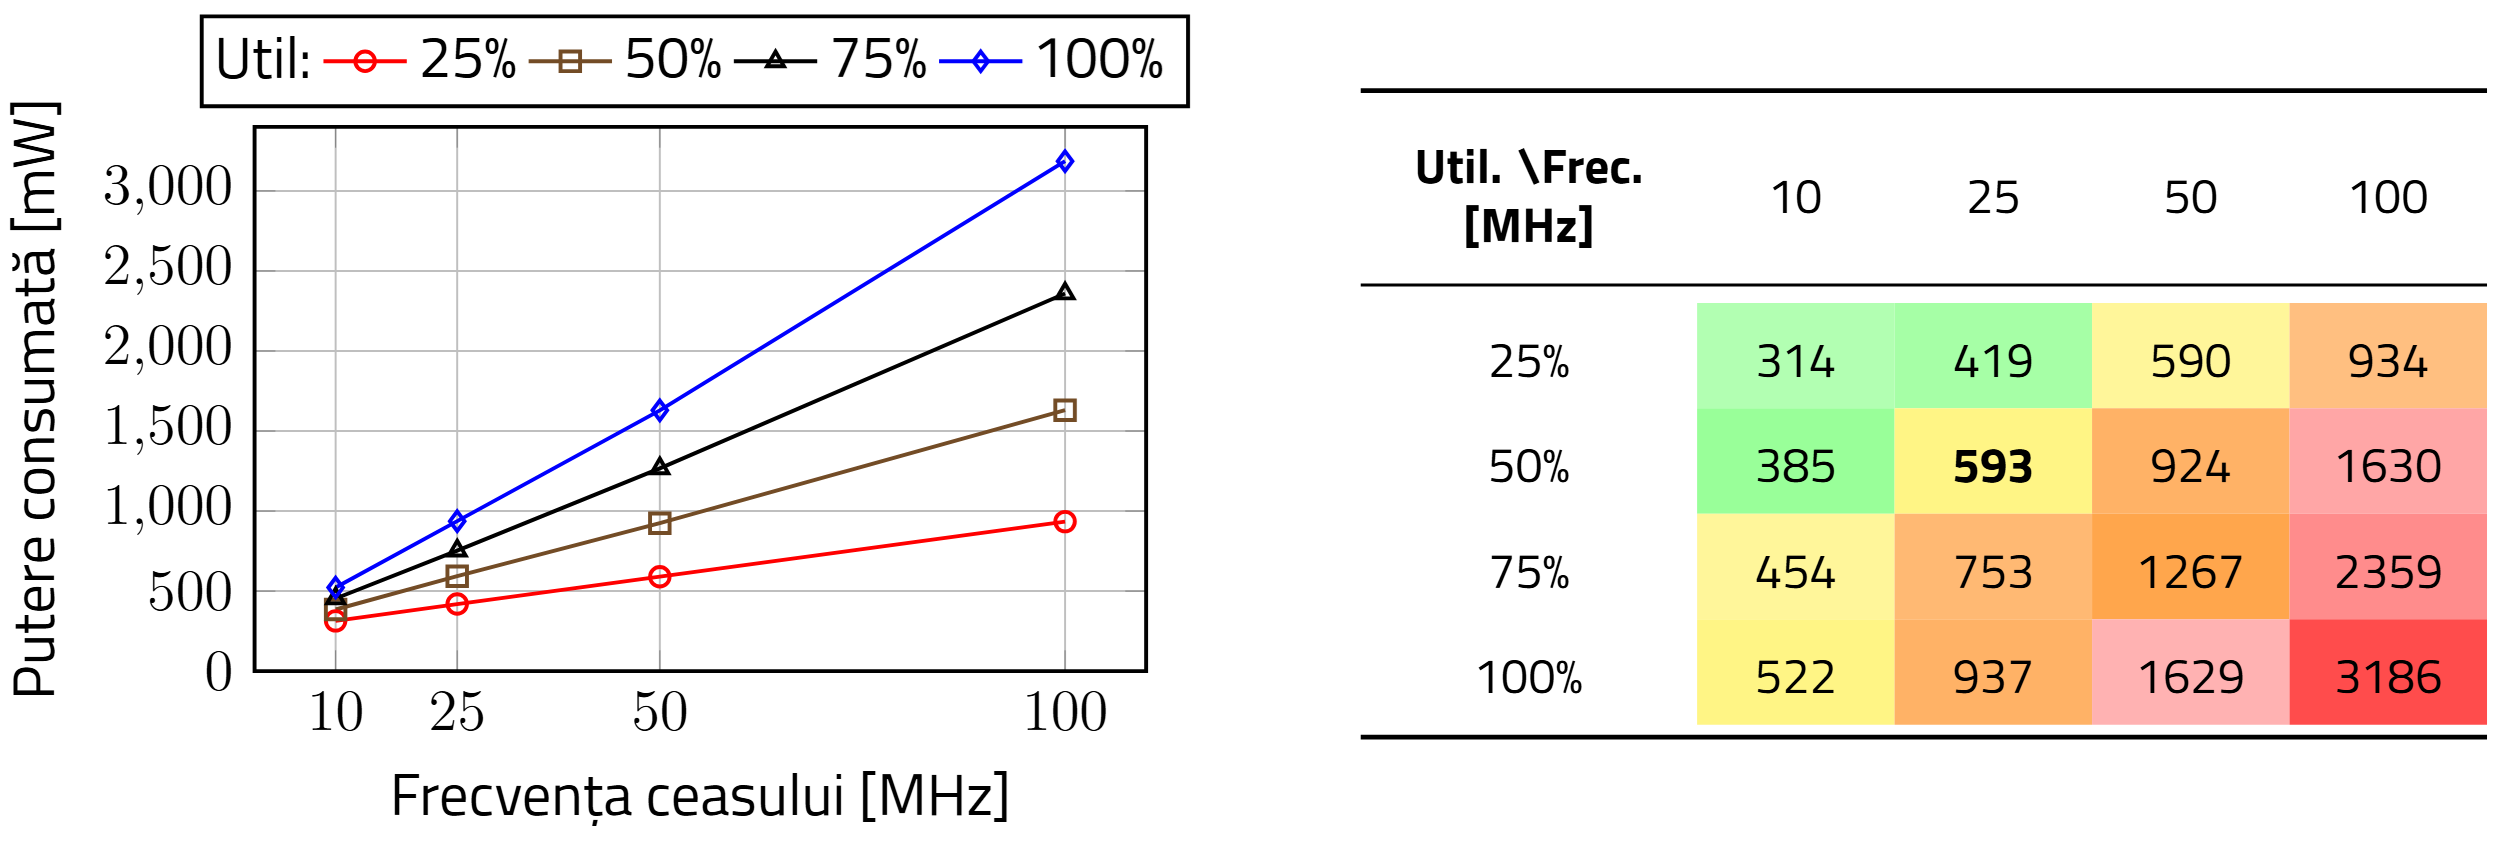
\includegraphics[width=\columnwidth]{./Images/ts_freq_vs_utiliz.png}
    \caption{Consumul FPGA-ului în funcție de frecvența proiectului și utilizarea memoriilor.}
    \label{fig:ts_freq_vs_utiliz}
\end{figure}

Al doilea set de teste a constat în compararea a patru configurații: un proiect de referință (50\% utilizare a memoriei și frecvența de 25 MHz), un proiect identic la care a fost activată opțiunea \textit{power\_opt\_design} la etapa de implementare, un proiect care include un microprocesor MicroBlaze pentru controlul logicii de detecție și corecție, și un al patrulea proiect care combină implementarea MicroBlaze cu optimizările avansate de consum. Opțiunea \textit{power\_opt\_design} aplică optimizări suplimentare față de setările implicite, precum tehnici de clock-gating \cite{ug907}. 

Rezultatele indică faptul că \textit{power\_opt\_design} are un impact redus asupra logicii relativ simple a modulului de detecție, reducerea consumului fiind sub 1\%. În schimb, pentru structuri mai complexe, precum procesorul MicroBlaze, efectul este mai vizibil, cu o reducere de până la 3.65\%. Introducerea MicroBlaze-ului a determinat o creștere a consumului de 20 mW față de proiectul fără procesor, evidențiind structura foarte bine optimizată al acestuia.

Testele privind influența frecvenței de scanare a memoriilor asupra consumului de curent au arătat că majoritatea consumului este de natură statică, reprezentând aproximativ 430 mA. Chiar și la o frecvența redusă de scanare de 12 Hz, consumul total se menține la 72.5\% din valoarea înregistrată la frecvența maximă de eșantionare de 12 kHz. 

Concluziile rezultate din aceste experimente sunt atât de natură hardware, cât și software. Din punct de vedere al configurației \gls{fpga}-ului, reducerea frecvenței semnalului de ceas este cea mai eficientă metodă de diminuare a consumului de energie, în timp ce menținerea unui grad ridicat de utilizare contribuie la maximizarea eficienței detectorului și, implicit, a secțiunii transversale. Deși frecvența de scanare are un impact redus asupra consumului total, aceasta trebuie aleasă astfel încât să nu afecteze rezoluția temporală a senzorului.

La nivel de \gls{pcb}, au fost implementate modificări pentru eliminarea consumatorilor auxiliari nenecesari, precum LED-urile de status și convertorul \gls{usb} la \gls{uart}/\gls{jtag}.

\section{Metodologia testării rezistenței la radiație}
Deși nu au fost realizate teste într-un mediu controlat de radiație, care să ofere valori de referință comparabile mai târziu cu măsurători experimentale din spațiu sau să permită evaluarea directă a eficacității senzorului, este posibilă pregătirea sistemului pentru misiune prin simulări și metode analitice. Acestea permit atât estimarea comportamentului sistemului în orbită, cât și definirea unor proceduri clare de prelucrare a datelor obținute experimental în rezultate standardizate și utilizabile. 

Există unelte de simulare suficient de avansate, validate experimental, și date publice suficiente pentru a estima parametrii mediului de radiație din orbita terestră joasă - \gls{leo}, precum și literatură de specialitate și documentații de la producători pentru evaluarea susceptibilității dispozitivelor \gls{fpga} la radiație. Combinând caracteristicile mediului cu cele ale dispozitivului țintă, se poate estima performanța ideală a sistemului la apariția evenimentelor de tip \gls{seu}. Mai concret, pe baza fluxurilor de particule și a secțiunii transversale asociate fiecărui tip de particulă și nivel de energie, se poate calcula rata de apariție a \gls{seu}-urilor pentru un anumit număr de biți sensibili și o perioadă de timp dată.

Pentru a clarifica interacțiunea dintre aceste mărimi fizice, termenii și efectele relevante vor fi explicate succint în următoarele paragrafe. Mai departe, vor fi explicate formulele de conversie a mărimilor fizice în \gls{seu}-uri pe secundă, vor fi prezentate spectrele de energii obținute cu uneltele de simulare și metodele folosite în literatură pentru determinarea secțiunii transversale. La final, vor fi expuse rezultatele obținute.

\subsection{Mărimile fizice și efectele asociate radiației}
Mediul spațial, inclusiv în orbita terestră joasă \gls{leo}, conține mai multe tipuri de particule energetice, caracterizate prin domenii diferite de energie, mecanisme diferite de apariție și moduri variate de interacțiune cu materia. Principalele surse de efecte de tip \gls{see} în \gls{leo} sunt electroni (\(e^-\)) și protoni (\(p^+\)) captați în magnetosfera terestră. Aceste particule provenite din vântul solar și din evenimente solare și, datorită sarcinii electrice, sunt prinse de câmpul magnetic al Pământului, formând regiuni de acumulare cunoscute sub numele de centurile Van Allen \cite{van_allen_belts}. Soarele este o sursă activă suplimentară de radiație, accelerând protoni, electroni și, mai rar, ioni grei, în timpul erupțiilor solare \cite{solar_radiation}. Aceste evenimente sunt sporadice și variabile în intensitate, fiind considerate o sursă secundară de radiație electromagnetică, în raport cu particulele capturate, care domină mediul de radiație în \gls{leo} \cite{space_radiation_enviroment}. 

Sursa principală de ioni grei este reprezentată de razele cosmice galactice - \gls{gcr}. Acestea sunt particule cu energii foarte mari, provenite din afara sistemului solar, generate de evenimente astrofizice extreme precum supernovele \cite{gcrs}. Compoziția lor este dominată de protoni și particule alfa (\(He^{2+}\)), însă o fracțiune mică este formată din ioni cu număr atomic mai mare (C, O, Ne, Mg, etc.). Deși rari, acești ioni sunt importanți datorită energiei foarte mare, care îi face extrem de eficienți în producerea efectelor asupra circuitelor electronice.

După cum se poate observa, nu a fost explicată interacțiunea cu cea de-a treia particulă elementară, neutronii (\(n^0\)). Aceștia nu sunt captați în magnetosfera Pământului, deoarece nu au o sarcină electrică (de unde și numele) și sunt instabili cât sunt particule libere, având un timp de înjumătățire (half-life) de aproximativ 15 minute, descompunându-se într-un proton, un electron și un antineutrino (\(\bar{\nu}_e\)). Deși neutronii nu au o prezență îndelungată, aceștia sunt totuși prezenți ca particule secundare, fiind generați în urma interacțiunilor nucleare dintre protoni sau ioni grei și atmosfera terestră sau materialele unui nanosatelit (fuzelaj, \gls{pcb}-uri etc.) \cite{space_radiation_enviroment}. Acești neutroni pot la rândul lor induce efecte asupra elementelor active ale sistemului. 

Toate aceste particule sunt caracterizate prin fluxul de particule \(\Phi [particule \cdot m^{-2} \cdot s^{-1}]\), care reprezintă numărul de particule ce traversează o unitate de suprafață într-o unitate de timp. În cazul mediului spațial, fluxul caracterizează intensitatea unui tip de particule într-un anumit volum și se utilizează de obicei fluxul omnidirecțional, presupunând o distribuire uniformă a direcțiilor de incidență. În practică, fluxul este descris prin fluxul diferențial de particule \(\Phi(E) [particule \cdot m^{-2} \cdot s^{-1} \cdot MeV^{-1}]\), exprimat în funcție de energie. Dacă fluxul de particule este integrat în timp, se obține fluența \(F [particule \cdot m^{-2}]\), care caracterizează expunerea totală de radiație sau probabilitatea apariției unui \gls{seu} pe durata unei misiuni.

Un alt parametru fundamental în evaluarea efectelor radiației este \gls{let} \( LET [MeV \cdot cm^2 \cdot g^{-1}]\), care exprimă cantitatea de energie depusă de o particulă pe unitatea de lungime într-un material. Valoarea \gls{let} depinde de tipul particulei, energia acesteia și proprietățile materialul traversat (puterea de oprire a materialului fiind afectată de densitatea și compoziția sa). Un \gls{let} ridicat implică o densitate mare de energie depozitată și o probabilitate crescută de apariției a efectelor de tip \gls{see}. Ionii grei proveniți din \gls{gcr}, deși au un flux redus, au valori pentru \gls{let} foarte mari, fiind capabili să producă direct un număr mare de \gls{see}-uri \cite{nasa_radiation_effects}. Protonii au un \gls{let} mai scăzut și generează de regulă \gls{see}-uri indirect, prin reacții secundare cu materialele din jurul circuitelor integrate.

Mărimile fizice descrise anterior caracterizează mediul de radiație. Pentru a evalua eficiența unui senzor de radiație, este necesară și caracterizarea susceptibilității dispozitivului activ. Aceasta este exprimată prin secțiunea transversală - cross-section \(\sigma [cm^2]\), care reprezintă probabilitatea ca o particulă să producă o interacțiune. În cazul memoriilor, se utilizează secțiunea transversală per bit \(\sigma(E) [cm^2 / bit]\), care exprimă probabilitatea ca o particulă cu o anumită energie să inducă un \gls{seu}. Această mărime se determină prin măsurători experimentale prin iradiere controlată și este independentă de fluxul de particule, permițând caracterizarea dispozitivului separat de mediul spațial. Determinarea experimentală este cea mai bună metodă pentru aflarea secțiunii transversale, deoarece depinde de numeroși factori, precum tipul și energia unei particule, tehnologia de fabricație și structura celulei de memorie și aria sensibilă totală.

\subsection{Metoda de conversie între mărimi fizice și rata SEU-urilor}
Rata de apariție a \gls{seu}-urilor este determinată de combinația dintre fluxul de particule și susceptibilitatea dispozitivului la acele particule, exprimată prin secțiunea transversală. Pentru o particulă cu o anumită energie, rata de \gls{seu}-uri se calculează ca:
\begin{equation}
R_{\mathrm{SEU}} =
\int_{0}^{\infty} \Phi(E)\,\sigma(E)\,\mathrm{d}E
\quad sau \quad 
R_{\mathrm{SEU}} =
\sum_{i=1}^{N}
\Phi(E_i)\,
\sigma(E_i)\,
\Delta E_i
\end{equation}
Ecuația reprezintă integrarea produsului dintre fluxul de particule și secțiunea transversală în funcție de energie. În practică, secțiunile transversale sunt obținute experimental pentru intervale discrete de energie, motiv pentru care varianta a doua este utilizată în majoritatea aplicațiilor.

Această formulare poate fi folosită pentru particule elementare, precum protonii și electronii. În cazul ionilor grei, probabilitatea de apariție a unui \gls{seu} nu este determinată direct de energia particulei, ci de cantitatea de energie depusă în volumul sensibil al dispozitivului. Acest fenomen este caracterizat prin \gls{let}, care descrie cantitatea de energie transferată materialului în urma traversării particulei \cite{space_radiation_enviroment}. În acest caz, rata de \gls{seu}-uri se exprimă ca:
\begin{equation}
R_{\mathrm{SEU},\mathrm{HI}} =
\int_{0}^{\infty}
\Phi(\mathrm{LET})\,
\sigma(\mathrm{LET})\,
\mathrm{d}(\mathrm{LET})
\quad sau \quad 
R_{\mathrm{SEU},\mathrm{HI}} =
\sum_{i=1}^{M}
\Phi(\mathrm{LET}_i)\,
\sigma(\mathrm{LET}_i)\,
\Delta \mathrm{LET}_i
\end{equation}

Fiecare dintre aceste expresii este valabilă pentru un singur tip de particulă. Prin urmare, rata totală de \gls{seu}-uri este obținută prin însumarea contribuțiilor individuale ale fiecărei particule:
\begin{equation}
R_{\mathrm{SEU,tot}} = R_{\mathrm{SEU, p^+}} + R_{\mathrm{SEU, e^-}} + R_{\mathrm{SEU, solar}} + R_{\mathrm{SEU, GCR}}
\end{equation}

Expresiile prezentate sunt implementate și în diferite unelte de simulare dezvoltate de \gls{nasa} sau \gls{esa}, care permit includerea unor parametrii suplimentari, precum grosimea fuzelajului satelitului, care poate oferii protecție împotriva radiației. De asemenea, secțiunile transversale în funcție de \gls{let} și energie pot fi introduse sub formă de funcții analitice (de exemplu Weibull), seturi de date experimentale sau aproximări hibride.

Datorită naturii integrale a expresiei ratei de \gls{seu}-uri, determinarea inversă a spectrului de \gls{let} sau a secțiunii transversale ale dispozitivului pornind de la o singură rată măsurată nu admite o soluție unică. O variantă des folosită constă în definirea unei secțiuni transversale efective, care concentrează toate efectele mediului și ale dispozitivului într-o singură valoare:
\begin{equation}
\sigma_{\mathrm{eff}} = \frac{R_{\mathrm{SEU}}}{\displaystyle \sum_k \Phi(x_k)\,\Delta x_k},
\end{equation}
unde \(x_k\) reprezintă energia pentru particulele elementare sau \gls{let} pentru ionii grei. Această mărime este valabilă doar pentru dispozitivul analizat și pentru mediul de radiație specific.

\subsection{Determinarea fluxurilor de particule în LEO}
Pentru estimarea fluxurilor de particule din mediul spațial sunt disponibile mai multe unelte dezvoltate de principalele agenții spațiale ale lumii. Acestea sunt adesea disponibile online pentru descărcare sau pentru utilizare directă și integrează diferite facilități și modele matematice validate pentru, simularea mediului de radiație. În cadrul acestui proiect a fost utilizată suita \gls{spenvis} \cite{spenvis}, dezvoltată de Institutul Regal Belgian pentru Aeronomie Spațială (BIRA-IASB) pentru \gls{esa}.

\gls{spenvis} permite definirea parametrilor ce descriu orbita care va fi parcursă de nanosatelit și a duratei misiunii, pe baza cărora pot fi rulate modele specifice standardizate pentru obținerea spectrelor de flux ale diferitelor tipuri de particule. Deoarece orbita finală a nanosatelitului nu este încă stabilită, au fost utilizați parametrii orbitei \gls{iss}, având în vedere că lansarea va avea loc din apropierea acesteia. Această abordare este uzuală pentru sateliți de tip CubeSat, care sunt frecvent lansați de pe \gls{iss} în cadrul misiunilor de aprovizionare ale stației spațiale. Au fost simulate fluxurile pentru electroni și protonii capturați în magnetosferă, particule provenite din evenimente solare, precum și ionii grei generați de raze cosmice galactice. Rezultatele simulărilor sunt prezentate în Figura \ref{fig:ts_leo_fluxes}.

% \begin{figure}[h]
%     \centering
%     \begin{tikzpicture}
%         \begin{loglogaxis}[
%             width=0.97\linewidth,
%             height=12cm,
%             xlabel={Energie [MeV]},
%             ylabel={Flux diferențial [\(m^-2 \,\, s^-1 \,\, MeV^-1\)]},
%             grid=major,
%             grid style={dashed,gray!30},
%             xticklabel style={
%                 /pgf/number format/sci,
%                 /pgf/number format/precision=2
%             },
%             enlarge x limits=0.05,
%             enlarge y limits=0.05,
%             legend style={at={(0.47,1.03)}, anchor=south, legend columns=6, column sep=7pt}
%         ]

%         %trapped electrons
%         \addplot[blue, line width=1.4pt, mark=o, mark size=2pt, mark repeat=6] coordinates {(4.0000E-02, 3.1961E+09) (1.0000E-01, 2.2345E+09) (2.0000E-01, 8.9920E+08) (3.0000E-01, 2.4616E+08) (4.0000E-01, 9.9612E+07) (5.0000E-01, 5.0574E+07) (6.0000E-01, 2.5251E+07) (7.0000E-01, 1.8114E+07) (8.0000E-01, 1.2934E+07) (1.0000E+00, 7.8209E+06) (1.2500E+00, 4.8235E+06) (1.5000E+00, 3.0873E+06) (1.7500E+00, 1.9804E+06) (2.0000E+00, 1.3465E+06) (2.2500E+00, 9.2006E+05) (2.5000E+00, 6.5509E+05) (2.7500E+00, 4.5648E+05) (3.0000E+00, 2.9596E+05) (3.2500E+00, 1.9906E+05) (3.5000E+00, 1.4035E+05) (3.7500E+00, 1.0111E+05) (4.0000E+00, 7.1117E+04) (4.2500E+00, 5.0349E+04) (4.5000E+00, 3.1433E+04) (4.7500E+00, 1.9766E+04) (5.0000E+00, 1.2267E+04) (5.5000E+00, 4.8950E+03) (6.0000E+00, 1.1842E+03) (6.5000E+00, 1.6726E+02)};
%         \addlegendentry{\(e^-\)}

%         %trapped protons
%         \addplot[red, line width=1.4pt, mark=square, mark size=2pt, mark repeat=6] coordinates {(1.0000E-01, 1.8633E+07) (1.5000E-01, 1.5087E+07) (2.0000E-01, 1.1760E+07) (3.0000E-01, 7.3154E+06) (4.0000E-01, 4.7234E+06) (5.0000E-01, 3.0487E+06) (6.0000E-01, 2.2705E+06) (7.0000E-01, 1.7405E+06) (1.0000E+00, 9.7617E+05) (1.5000E+00, 4.5203E+05) (2.0000E+00, 2.8014E+05) (3.0000E+00, 1.2733E+05) (4.0000E+00, 7.2643E+04) (5.0000E+00, 4.2957E+04) (6.0000E+00, 2.8390E+04) (7.0000E+00, 1.8902E+04) (1.0000E+01, 9.7805E+03) (1.5000E+01, 3.9341E+03) (2.0000E+01, 2.4733E+03) (3.0000E+01, 1.5711E+03) (4.0000E+01, 1.2667E+03) (5.0000E+01, 1.2090E+03) (6.0000E+01, 1.1998E+03) (7.0000E+01, 1.0922E+03) (1.0000E+02, 8.1883E+02) (1.5000E+02, 4.7073E+02) (2.0000E+02, 2.5157E+02) (3.0000E+02, 8.2076E+01)};
%         \addlegendentry{\(p^+\)}

%        %solar protons
%        \addplot[black, line width=1.4pt, mark=triangle, mark size=2.5pt, mark repeat=8] coordinates {(1.0000E-01, 4.5876E+04) (1.1000E-01, 4.1606E+04) (1.2000E-01, 3.8055E+04) (1.4000E-01, 3.2493E+04) (1.6000E-01, 2.8336E+04) (1.8000E-01, 2.5113E+04) (2.0000E-01, 2.2542E+04) (2.2000E-01, 2.0444E+04) (2.5000E-01, 1.7933E+04) (2.8000E-01, 1.5966E+04) (3.2000E-01, 1.3924E+04) (3.5000E-01, 1.2702E+04) (4.0000E-01, 1.1077E+04) (4.5000E-01, 9.8170E+03) (5.0000E-01, 8.8120E+03) (5.5000E-01, 7.9918E+03) (6.3000E-01, 6.9532E+03) (7.1000E-01, 6.1513E+03) (8.0000E-01, 5.4429E+03) (9.0000E-01, 4.8239E+03) (1.0000E+00, 4.3300E+03) (1.1000E+00, 3.9270E+03) (1.2000E+00, 3.5919E+03) (1.4000E+00, 3.0669E+03) (1.6000E+00, 2.6745E+03) (1.8000E+00, 2.3704E+03) (2.0000E+00, 2.1277E+03) (2.2000E+00, 1.9004E+03) (2.5000E+00, 1.6332E+03) (2.8000E+00, 1.4279E+03) (3.2000E+00, 1.2119E+03) (3.5000E+00, 1.0810E+03) (4.0000E+00, 9.1173E+02) (4.5000E+00, 7.7549E+02) (5.0000E+00, 6.7097E+02) (5.5000E+00, 5.8383E+02) (6.3000E+00, 4.7747E+02) (7.1000E+00, 3.9785E+02) (8.0000E+00, 3.2942E+02) (9.0000E+00, 2.7156E+02) (1.0000E+01, 2.2770E+02) (1.1000E+01, 1.9027E+02) (1.2000E+01, 1.6150E+02) (1.4000E+01, 1.2079E+02) (1.6000E+01, 9.3922E+01) (1.8000E+01, 7.5230E+01) (2.0000E+01, 6.1684E+01) (2.2000E+01, 5.0150E+01) (2.5000E+01, 3.7992E+01) (2.8000E+01, 2.9703E+01) (3.2000E+01, 2.1923E+01) (3.5000E+01, 1.7706E+01) (4.0000E+01, 1.2878E+01) (4.5000E+01, 9.5936E+00) (5.0000E+01, 7.3723E+00) (5.5000E+01, 5.7311E+00) (6.3000E+01, 3.9846E+00) (7.1000E+01, 2.8697E+00) (8.0000E+01, 2.0530E+00) (9.0000E+01, 1.4558E+00) (1.0000E+02, 1.0638E+00) (1.1000E+02, 7.8673E-01) (1.2000E+02, 5.9728E-01) (1.4000E+02, 3.6662E-01) (1.6000E+02, 1.2312E+00) (1.8000E+02, 3.4931E+00) (2.0000E+02, 4.6094E+00) (2.2000E+02, 4.7979E+00) (2.5000E+02, 4.4255E+00) (2.8000E+02, 3.8298E+00) (3.2000E+02, 3.0445E+00) (3.5000E+02, 2.5964E+00) (4.0000E+02, 2.1176E+00) (4.5000E+02, 1.7047E+00) (5.0000E+02, 1.3661E+00)};
%        \addlegendentry{\(p^+\) Solari}

%        %solar ions
%        \addplot[brown, line width=1.4pt, mark=diamond, mark size=2.5pt, mark repeat=8] coordinates {(1.0000E-01, 4.4784E+03) (1.1000E-01, 3.9534E+03) (1.2000E-01, 3.5281E+03) (1.4000E-01, 2.8837E+03) (1.6000E-01, 2.4215E+03) (1.8000E-01, 2.0757E+03) (2.0000E-01, 1.8084E+03) (2.2000E-01, 1.5964E+03) (2.5000E-01, 1.3506E+03) (2.8000E-01, 1.1645E+03) (3.2000E-01, 9.7784E+02) (3.5000E-01, 8.6967E+02) (4.0000E-01, 7.3027E+02) (4.5000E-01, 6.2599E+02) (5.0000E-01, 5.4539E+02) (5.5000E-01, 4.8145E+02) (6.3000E-01, 4.0308E+02) (7.1000E-01, 3.4473E+02) (8.0000E-01, 2.9489E+02) (9.0000E-01, 2.5278E+02) (1.0000E+00, 2.2023E+02) (1.1000E+00, 1.9442E+02) (1.2000E+00, 1.7350E+02) (1.4000E+00, 1.4181E+02) (1.6000E+00, 1.1908E+02) (1.8000E+00, 1.0208E+02) (2.0000E+00, 8.8934E+01) (2.2000E+00, 7.6849E+01) (2.5000E+00, 6.3179E+01) (2.8000E+00, 5.3107E+01) (3.2000E+00, 4.2816E+01) (3.5000E+00, 3.6767E+01) (4.0000E+00, 2.9302E+01) (4.5000E+00, 2.3637E+01) (5.0000E+00, 1.9504E+01) (5.5000E+00, 1.6227E+01) (6.3000E+00, 1.2443E+01) (7.1000E+00, 9.7790E+00) (8.0000E+00, 7.5869E+00) (9.0000E+00, 5.8698E+00) (1.0000E+01, 4.6287E+00) (1.1000E+01, 3.3945E+00) (1.2000E+01, 2.5575E+00) (1.4000E+01, 1.5488E+00) (1.6000E+01, 1.0030E+00) (1.8000E+01, 6.8369E-01) (2.0000E+01, 4.8526E-01) (2.2000E+01, 3.3896E-01) (2.5000E+01, 2.0948E-01) (2.8000E+01, 1.3673E-01) (3.2000E+01, 8.2628E-02) (3.5000E+01, 5.8892E-02) (4.0000E+01, 6.1688E-02) (4.5000E+01, 2.5585E-01) (5.0000E+01, 4.1676E-01) (5.5000E+01, 4.5522E-01) (6.3000E+01, 4.2000E-01) (7.1000E+01, 3.5537E-01) (8.0000E+01, 2.8518E-01) (9.0000E+01, 2.2038E-01) (1.0000E+02, 1.7646E-01) (1.1000E+02, 1.4651E-01) (1.2000E+02, 1.2488E-01) (1.4000E+02, 9.0114E-02) (1.6000E+02, 6.5831E-02) (1.8000E+02, 4.9090E-02) (2.0000E+02, 3.7273E-02) (2.2000E+02, 2.8902E-02) (2.5000E+02, 2.0357E-02) (2.8000E+02, 1.4817E-02) (3.2000E+02, 1.0137E-02) (3.5000E+02, 7.8400E-03) (4.0000E+02, 5.3238E-03) (4.5000E+02, 3.7707E-03) (5.0000E+02, 2.7655E-03)};
%        \addlegendentry{\(He^{2+}\) Solari}

%         %GCR - H
%         \addplot[green, line width=1.4pt, mark=+, mark size=3pt, mark repeat=8] coordinates {(1.0000E+00, 8.7175E-08) (1.1000E+00, 1.0590E-07) (1.2000E+00, 1.2637E-07) (1.4000E+00, 1.7243E-07) (1.6000E+00, 2.2513E-07) (1.8000E+00, 2.8427E-07) (2.0000E+00, 3.4965E-07) (2.2000E+00, 4.2105E-07) (2.5000E+00, 5.3905E-07) (2.8000E+00, 6.6958E-07) (3.2000E+00, 8.6214E-07) (3.5000E+00, 1.0198E-06) (4.0000E+00, 1.3061E-06) (4.5000E+00, 1.6203E-06) (5.0000E+00, 1.9605E-06) (5.5000E+00, 2.3248E-06) (6.3000E+00, 2.9542E-06) (7.1000E+00, 3.6360E-06) (8.0000E+00, 4.4592E-06) (9.0000E+00, 5.4366E-06) (1.0000E+01, 6.4728E-06) (1.1000E+01, 7.5613E-06) (1.2000E+01, 8.6964E-06) (1.4000E+01, 1.1087E-05) (1.6000E+01, 1.3611E-05) (1.8000E+01, 1.6241E-05) (2.0000E+01, 1.8955E-05) (2.2000E+01, 2.1734E-05) (2.5000E+01, 2.5992E-05) (2.8000E+01, 3.0321E-05) (3.2000E+01, 3.6147E-05) (3.5000E+01, 4.0523E-05) (4.0000E+01, 4.7773E-05) (4.5000E+01, 5.4911E-05) (5.0000E+01, 6.1886E-05) (5.5000E+01, 6.8665E-05) (6.3000E+01, 7.9047E-05) (7.1000E+01, 8.8810E-05) (8.0000E+01, 9.9024E-05) (9.0000E+01, 1.0941E-04) (1.0000E+02, 1.1882E-04) (1.1000E+02, 1.2728E-04) (1.2000E+02, 1.3486E-04) (1.4000E+02, 1.4760E-04) (1.6000E+02, 8.0730E-04) (1.8000E+02, 3.4848E-03) (2.0000E+02, 6.6356E-03) (2.2000E+02, 9.7996E-03) (2.5000E+02, 1.4294E-02) (2.8000E+02, 1.8376E-02) (3.2000E+02, 2.3207E-02) (3.5000E+02, 2.6975E-02) (4.0000E+02, 3.4507E-02) (4.5000E+02, 4.2190E-02) (5.0000E+02, 4.8713E-02) (5.5000E+02, 5.3983E-02) (6.3000E+02, 6.0823E-02) (7.1000E+02, 6.5769E-02) (8.0000E+02, 6.9676E-02) (9.0000E+02, 7.2441E-02) (1.0000E+03, 7.4015E-02) (1.1000E+03, 7.4707E-02) (1.2000E+03, 7.4796E-02) (1.4000E+03, 7.3643E-02) (1.6000E+03, 7.1518E-02) (1.8000E+03, 6.8972E-02) (2.0000E+03, 6.6414E-02) (2.2000E+03, 6.4005E-02) (2.5000E+03, 6.0132E-02) (2.8000E+03, 5.6155E-02) (3.2000E+03, 5.1066E-02) (3.5000E+03, 4.7260E-02) (4.0000E+03, 4.1330E-02) (4.5000E+03, 3.6119E-02) (5.0000E+03, 3.1634E-02) (5.5000E+03, 2.7827E-02) (6.3000E+03, 2.2976E-02) (7.1000E+03, 1.9335E-02) (8.0000E+03, 1.6448E-02) (9.0000E+03, 1.3854E-02) (1.0000E+04, 1.1587E-02) (1.1000E+04, 9.7308E-03) (1.2000E+04, 8.1933E-03) (1.4000E+04, 5.9283E-03) (1.6000E+04, 4.4161E-03) (1.8000E+04, 3.3594E-03) (2.0000E+04, 2.6138E-03) (3.0000E+04, 9.4845E-04) (4.0000E+04, 4.5007E-04) (5.0000E+04, 2.5014E-04) (6.0000E+04, 1.5415E-04) (7.0000E+04, 1.0217E-04) (8.0000E+04, 7.1456E-05) (9.0000E+04, 5.2085E-05) (1.0000E+05, 3.9228E-05)};
%         \addlegendentry{\(p^+\) GCR}

%         %GCR - He
%         \addplot[purple, line width=1.4pt, mark=star, mark size=3pt, mark repeat=8] coordinates {(1.0000E+00, 6.6710E-08) (1.1000E+00, 8.0268E-08) (1.2000E+00, 9.4890E-08) (1.4000E+00, 1.2715E-07) (1.6000E+00, 1.6317E-07) (1.8000E+00, 2.0267E-07) (2.0000E+00, 2.4538E-07) (2.2000E+00, 2.9106E-07) (2.5000E+00, 3.6469E-07) (2.8000E+00, 4.4391E-07) (3.2000E+00, 5.5723E-07) (3.5000E+00, 6.4739E-07) (4.0000E+00, 8.0623E-07) (4.5000E+00, 9.7438E-07) (5.0000E+00, 1.1505E-06) (5.5000E+00, 1.3333E-06) (6.3000E+00, 1.6374E-06) (7.1000E+00, 1.9529E-06) (8.0000E+00, 2.3182E-06) (9.0000E+00, 2.7334E-06) (1.0000E+01, 3.1553E-06) (1.1000E+01, 3.5813E-06) (1.2000E+01, 4.0094E-06) (1.4000E+01, 4.8656E-06) (1.6000E+01, 5.7142E-06) (1.8000E+01, 6.5489E-06) (2.0000E+01, 7.3654E-06) (2.2000E+01, 8.1608E-06) (2.5000E+01, 9.3107E-06) (2.8000E+01, 1.0406E-05) (3.2000E+01, 1.1779E-05) (3.5000E+01, 1.2744E-05) (4.0000E+01, 2.4693E-05) (4.5000E+01, 1.7491E-04) (5.0000E+01, 4.5723E-04) (5.5000E+01, 7.6074E-04) (6.3000E+01, 1.2683E-03) (7.1000E+01, 1.7926E-03) (8.0000E+01, 2.3825E-03) (9.0000E+01, 2.9993E-03) (1.0000E+02, 3.6973E-03) (1.1000E+02, 4.5102E-03) (1.2000E+02, 5.4358E-03) (1.4000E+02, 7.1643E-03) (1.6000E+02, 8.7170E-03) (1.8000E+02, 1.0104E-02) (2.0000E+02, 1.1304E-02) (2.2000E+02, 1.2377E-02) (2.5000E+02, 1.3736E-02) (2.8000E+02, 1.4846E-02) (3.2000E+02, 1.6026E-02) (3.5000E+02, 1.6735E-02) (4.0000E+02, 1.7623E-02) (4.5000E+02, 1.8241E-02) (5.0000E+02, 1.8651E-02) (5.5000E+02, 1.8904E-02) (6.3000E+02, 1.9083E-02) (7.1000E+02, 1.9080E-02) (8.0000E+02, 1.8995E-02) (9.0000E+02, 1.8721E-02) (1.0000E+03, 1.8282E-02) (1.1000E+03, 1.7747E-02) (1.2000E+03, 1.7170E-02) (1.4000E+03, 1.5838E-02) (1.6000E+03, 1.4430E-02) (1.8000E+03, 1.3080E-02) (2.0000E+03, 1.1835E-02) (2.2000E+03, 1.0708E-02) (2.5000E+03, 9.2567E-03) (2.8000E+03, 8.0678E-03) (3.2000E+03, 6.8223E-03) (3.5000E+03, 6.1209E-03) (4.0000E+03, 5.1794E-03) (4.5000E+03, 4.3345E-03) (5.0000E+03, 3.6358E-03) (5.5000E+03, 3.0585E-03) (6.3000E+03, 2.3456E-03) (7.1000E+03, 1.8356E-03) (8.0000E+03, 1.4181E-03) (9.0000E+03, 1.0872E-03) (1.0000E+04, 8.5090E-04) (1.1000E+04, 6.7813E-04) (1.2000E+04, 5.4938E-04) (1.4000E+04, 3.7493E-04) (1.6000E+04, 2.6775E-04) (1.8000E+04, 1.9824E-04) (2.0000E+04, 1.5110E-04) (3.0000E+04, 5.2140E-05) (4.0000E+04, 2.4209E-05) (5.0000E+04, 1.3284E-05) (6.0000E+04, 8.1138E-06) (7.0000E+04, 5.3399E-06) (8.0000E+04, 3.7129E-06) (9.0000E+04, 2.6929E-06) (1.0000E+05, 2.0195E-06)};
%         \addlegendentry{\(He^{2+}\) GCR}

%     \end{loglogaxis}
%     \end{tikzpicture}
% \caption{Fluxul diferențial al particulelor din LEO: electroni, protoni, ioni solari și GCR.}%
% \label{fig:fpga_power_estimations}
% \end{figure}

\begin{figure}[ht!]
    \centering
    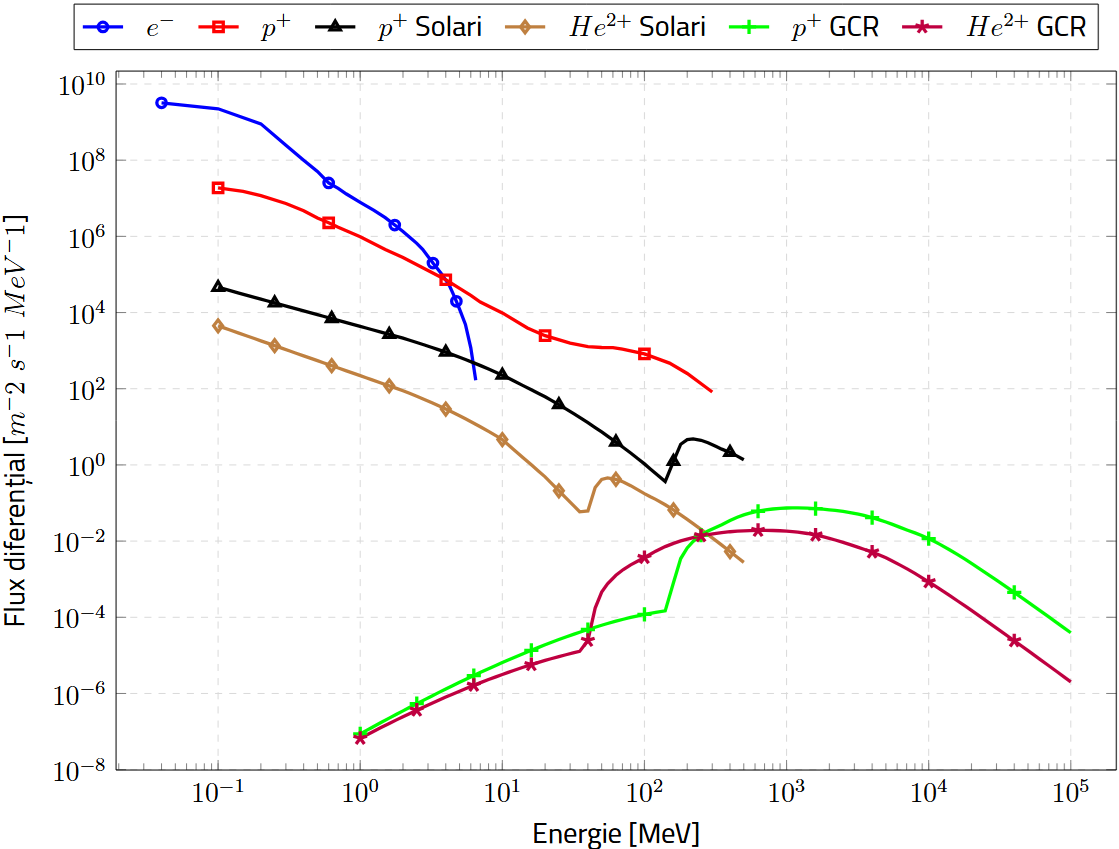
\includegraphics[width=\columnwidth]{./Images/ts_leo_fluxes.png}
    \caption{Fluxul diferențial al particulelor din LEO: electroni, protoni, ioni solari și GCR.}%
    \label{fig:ts_leo_fluxes}
\end{figure}

Fluxurile particulelor capturate, ale particulelor din evenimente solare și ale \gls{gcr}-urilor au fost evaluate folosind modelele AE8/AP8, CREME-96 și ISO-15390, fiind analizate fluxurile pentru \(p^+\), \(He^{2+}\) și \(e^-\). Pentru particulele captate și \gls{gcr} a fost folosită condiția de minim solar, corespunzătoare unei activități solare reduse și unui nivel maxim al radiației de la particulele capturate.

Se observă că fluxurile de protoni și electroni capturați sunt dominante, urmate de cele provenite din evenimente solare și, în final, de raze cosmice galactice. Totuși, aceste valori nu pot fi analizate izolat. Deși fluxurile \gls{gcr} sunt cu aproximativ șase ordine de mărime mai mici decât cele ale particulelor capturate, ionii grei din \gls{gcr} pot produce \gls{see}-uri direct, datorită valorilor ridicate ale \gls{let}-ului, mult mai mari decât cele protonilor capturați. 

Fluxurile de origine solară sunt foarte dependente de faza ciclului solar și de apariția unor evenimente sporadice, variind semnificativ atât în timp, cât și în intensitate. Din acest motiv, contribuția lor este de regulă considerată secundară în evaluările pe termen lung ale mediului spațial, comparativ cu fluxurile mai stabile ale particulelor capturate și ale \gls{gcr}-urilor.

Din figură rezultă că fluxul de electroni capturați este cel mai ridicat din mediul spațial. Totuși, aceștia au energii relativ scăzute, spectrul fiind puternic atenuat peste 10 MeV. Aceste energii sunt prea mici pentru a produce efecte relevante asupra dispozitivelor electronice, motiv pentru care electronii vor fi excluși din calculele ratei de \gls{seu}-uri. În \cite{electron_caused_seus_2} s-a arătat că \gls{seu}-urile induse de electroni pot apărea în dispozitive alimentate sub tensiunea nominală, de exemplu de la 1.2 V la 0.672 V. De asemenea, Matthew J. Gadlage et al. au raportat în \cite{electron_caused_seus} apariția \gls{seu}-urilor în tehnologii de 45 nm și 28 nm alimentate la tensiunea nominală, însă pentru energii ale electronilor peste 20 MeV, valori care depășesc domeniul întâlnit în \gls{leo}.

\subsection{Determinarea secțiunii transversale la radiație}
Determinarea secțiunii transversale a unui anumit dispozitiv este mult mai dificilă decât estimarea fluxurilor de particule. Într-un scenariu ideal, dispozitivul ar trebui expus la o sursă care emite un singur tip de particule, cu energie controlată și variabilă, pentru a obține spectrul complet al secțiunii transversale. Acest proces ar trebui repetat pentru fiecare tip de particulă de interes. În practică, însă, sursele terestre de radiație furnizează fluxuri mixte, cu domenii mari de energii (de ordinul sutelor de MeV), iar rezultatele experimentale publicate sunt adesea incomplete, limitate la una sau câteva valori reprezentative. Din aceste motive, valorile utilizate în continuare sunt aproximative, preluate din literatură, și trebuie interpretate cu un gram de scepticism.

Xilinx raportează, în cadrul testelor de calificare pentru \gls{fpga}-uri, o secțiune transversală de \(6.32 \times 10^-15 \; cm^2/bit\), conform raportului de fiabilitate \cite{amd_reliability_report}. Această valoare a fost determinată în urmă expunerii la un flux de neutroni generat la centrul \acrfull{lansce}. Conform documentației \gls{lansce}, spectrul energetic al neutronilor este foarte similar celui al protonilor capturați din \gls{leo} \cite{lansce_ice2}. Deși neutronii și protonii sunt particule diferite, mecanismele de apariție a efectelor \gls{see} sunt comparabile, permițând utilizarea acestor rezultate ca estimare a susceptibilității dispozitivului la \gls{see}-urile induse indirect.

C. Weulersse et al. \cite{metis_cross_section_simulation} au determinat parametrii Weibull ai secțiunii transversale pentru un \gls{fpga} din familia Kintex-7 (28 nm), utilizând uneltele de simulare METIS, SIMPA și PROFIT. Pentru un flux de protoni cu energii de până la 200 MeV, secțiunea transversală a fost estimată la aproximativ \(9 \times 10^-15 \; cm^2/bit\). În cazul ionilor grei, valorile raportate sunt semnificativ mai mari: aproximativ \(7.94 \times 10^-9 \; cm^2/bit\) pentru memoria \gls{bram} și \(1.43 \times 10^-9 \; cm^2/bit\) pentru memoria \gls{cram}. Aceste rezultate evidențiază faptul ca ionii grei reprezintă principala sursă de  \gls{see}-uri, având un impact mult mai mare decât protonii.

Rezultate similare au fost obținute în urma testelor efectuate la ciclotronul K500 de la Universitatea Texas A\&M, asupra \gls{fpga}-urilor Kintex-7 și UltraScale. Aceste studii confirmă că secțiunea transversală pentru ionii grei se află în intervalul \(10^{-9} - 10^{-8} \; cm^2/bit\) \cite{texas_ion_testing_1, texas_ion_testing_2}.

\subsection{Rezultate obținute}
Calculul ratei de apariție a \gls{seu}-urilor în funcție de fluxul de particule și în funcție de secțiunea transversală poate fi realizat fie analitic, fie cu ajutorul unor unelte specializate. În acest proiect a fost utilizat modulul "Short-term \gls{seu} rates" din cadrul uneltei \gls{spenvis}. Acesta permite estimarea ratelor de \gls{seu}-uri pentru protoni și ioni grei folosind diferite modele pentru secțiunea transversală (parametrii Weibull, date experimentale sau modele hibride), luând în considerare atât materialul activ al cipului (siliciu, prin intermediul SRIM2008), cât și grosimea echivalentă a stratului de protecție al fuzelajului. Deși \gls{fpga}-ul este plasat la capătul nanosatelitului și este, în mare parte, expus direct mediului spațial, interacțiunile particulelor cu structura internă a nanosatelitului pot genera radiații secundare care ajung la dispozitiv din direcții neexpuse direct.

Rezultatele obținute sunt prezentate în Tabelul \ref{tab:ts_seu_rates}. Primele trei rânduri corespund ratelor de \gls{seu}-uri pentru memoria de configurare a \gls{fpga}-ului, iar următoarele trei pentru memoria \gls{bram}. Ratele totale de \gls{seu}-uri la nivel de dispozitiv au fost determinate prin înmulțirea ratelor simulate cu dimensiunea fiecărei memorii (77.845.216 biți pentru \gls{cram} și 13.455.360 biți pentru \gls{bram}). Se observă că introducerea unui strat echivalent de protecție conduce la o reducere a ratelor de \gls{seu}-uri cu peste trei ordine de mărime. În aceste condiții, rata estimată de apariție a \gls{seu}-urilor pentru întregul dispozitiv scade sub un eveniment pe zi.

\begin{table}[h]
% BRAM bits = 13455360
% CRAM bits = 77845216
    \footnotesize
    \centering
    \renewcommand{\arraystretch}{1.6}
    \caption{Ratele de SEU-uri pentru memoria CRAM și BRAM a FPGA-ului Artix-7.}%
    \label{tab:ts_seu_rates}
    \begin{tabular}{C{1cm} C{2.8cm} C{2.5cm} C{2.5cm} C{2.8cm} C{2.8cm}}
		\toprule
			\textbf{Tip} & 
            \textbf{Grosime Al [mm]} & 
            \textbf{SEU/s/bit} &
            \textbf{SEU/zi/bit} &
            \textbf{SEU/s/dispozitiv} &
            \textbf{SEU/zi/dispozitiv} \\
		\midrule
            CRAM & 0.0  & 2.4121E-11 & 2.0841E-6 & 1.8777E-03 & 162.24 \\
		    CRAM & 0.1  & 2.2651E-14 & 1.9570E-9 & 1.7633E-06 & 0.152  \\
		    CRAM & 0.2  & 1.9412E-14 & 1.6772E-9 & 1.5111E-06 & 0.131  \\
		\midrule
		    BRAM & 0.0  & 1.0509E-8  & 9.0801E-4 & 1.4140E-01 & 12218  \\
		    BRAM & 0.1  & 7.2297E-13 & 6.2465E-8 & 9.7278E-06 & 0.840  \\
		    BRAM & 0.2  & 2.2682E-13 & 1.9597E-8 & 3.0519E-06 & 0.264  \\
		\bottomrule
    \end{tabular}
\end{table}

\chapter{Concluzii}
Obiectivul acestui proiect a fost utilizarea unui dispozitiv \acrlong{fpga} pentru realizarea unui senzor inteligent de radiație cosmică. A fost necesară dezvoltarea unei plăci suport care să faciliteze alimentarea și comunicația cu \gls{fpga}-ul, precum și integrarea acestuia într-un nanosatelit. În ansamblu, sistemul trebuie să respecte cerințe stricte pentru compatibilitatea cu platforma satelitară: \gls{pcb}-ul trebuie sa aibă un consum energetic scăzut și sa fie proiectat pentru a rezista mediului extrem spațial. De asemenea, configurația Verilog a \gls{fpga}-ului trebuie sa permită scanarea memoriilor, precum și comunicația cu mediul exterior. Toate aceste circuite trebuie să fie eficiente energetic, să utilizeze optim resursele și să fie rezistente la efectele radiației.

Algoritmul implementat pentru detecția \gls{seu}-urilor constă în scrierea unor secvențe cunoscute de biți de 0 și 1 în memoriile \gls{bram}, urmată de scanarea periodică a acestora și compararea valorilor citite cu cele nominale. În cazul detectării unei erori, aceasta este capturată și stocată într-un \gls{fifo} de ieșire, iar valoarea afectată este corectată. Biții modificați, împreună cu adresa de memorie, indexul blocului de memorie afectat și numărul scanării la care a fost identificată eroarea, sunt extrase din \gls{fifo} și transmise către \gls{obc}-ul local al nanosatelitului prin interfața \gls{lvds} \gls{spi}. Toate aceste module au fost implementate folosind tehnici de mitigare a efectelor radiației, precum registrele \gls{tmr} și coduri de detectare și corectare a erorilor (\gls{ecc}, \gls{crc} și checksum).

Placa suport a fost dezvoltată în două iterații: o versiune prototip și o versiune finală. Acestea includ circuite de alimentare ale \gls{fpga}-ului, realizate prin patru regulatoare de tensiune monitorizate cu senzori de curent prin interfața \gls{i2c}, circuite de configurare precum convertorul \gls{usb} la \gls{uart}/\gls{jtag} și o memorie non-volatilă de tip NOR FLASH, precum și circuite de comunicație cu exteriorul, incluzând conectori, un \gls{io}-Expander și convertorul menționat.

Atât componentele hardware, cât și software au fost supuse unor teste extinse de validare și simulare pentru a asigura fiabilitatea sistemului. Toate modulele \gls{fpga}-ului au fost simulate pentru identificarea erorilor logice sau de proiectare, urmate de validări fizice prin configurarea și testarea efectivă a dispozitivului. Au fost realizate analize detaliate ale consumului de curent pentru identificarea elementelor cu impact energetic mare și optimizarea sistemului, precum și măsurători de integritate a semnalelor și a alimentării \gls{pcb}-ului, atât în condiții nominale, cât și în scenarii extreme, cu utilizare maximă a resurselor \gls{fpga}-ului.

În final, a fost realizată o analiză a mediului specific orbitei joase a Pământului (\gls{leo}) și a modului în care acesta interacționează cu circuitele electronice. Au fost efectuate simulări pentru determinarea fluxurilor de particule caracteristice acestui mediu și pentru estimarea susceptibilității la radiație a \gls{fpga}-ului utilizat. Pe baza acestor date, a fost realizată o simulare pentru a calcula rata de apariție a evenimentelor \gls{seu} pentru dispozitivul țintă în \gls{leo}, în special pentru condițiile corespunzătoare orbitei \gls{iss}.

\section{Rezultate}
Rezultatele acestui proiect sunt în general pozitive și sunt susținute de rezultate obținute în urma testărilor experimentale. Atât partea software, cât și suportul hardware au fost dezvoltate și validate cu succes. Proiectul Verilog pentru dispozitivul \gls{fpga} a fost simulat și verificat fără erori funcționale, iar modulele de comunicație au fost testate cu succes prin interfațarea cu mai multe dispozitive externe. Ambele versiuni ale \gls{pcb}-ului au fost proiectate, fabricate și livrate, fiind complet funcționale. Problemele identificate în prima versiune au fost corectate în cea de-a doua, aceasta având caracteristici de semnal mai bune și un consum de energie mai redus. Analizele de integritate a semnalului și integritate a alimentării se află în limitele nominale, iar placa este compatibilă și pregătită pentru integrarea în nanosatelitul țintă.

În cadrul proiectului \gls{aicors} a fost dezvoltată o placă senzor de radiație cosmică ce urmează să fie integrată,  pe parcursul anului 2026, într-un nanosatelit de tip 3U (10 cm $\times$ 10 cm $\times$ 34 cm) destinat experimentelor academice, care va fi lansat către \gls{iss} cu ajutorul unei misiuni de reaprovizionare aparținând \gls{jaxa}. Nanosatelitul BIRDS-RPM este dezvoltat de Institutul de Tehnologie Kyushu, în cadrul programului internațional BIRDS, în colaborare cu Universitatea Tehnică a Moldovei și alte două instituții din Rwanda și Paraguay \cite{birds_manual}. Structura acestuia este prezentată în Figura \ref{fig:conclusion_birds_sat}, unde se poate observa, în partea stângă, payload-ul moldovenesc, ce include placa \gls{aicors}, poziționată la exterior, o placă cu nanosenzori, o placă de referință pentru măsurători de radiație, precum și \gls{obc}-ul local. Restul componentelor aparțin subsistemelor de control și comunicație ale nanosatelitului.

\begin{figure}[ht!]
    \centering
    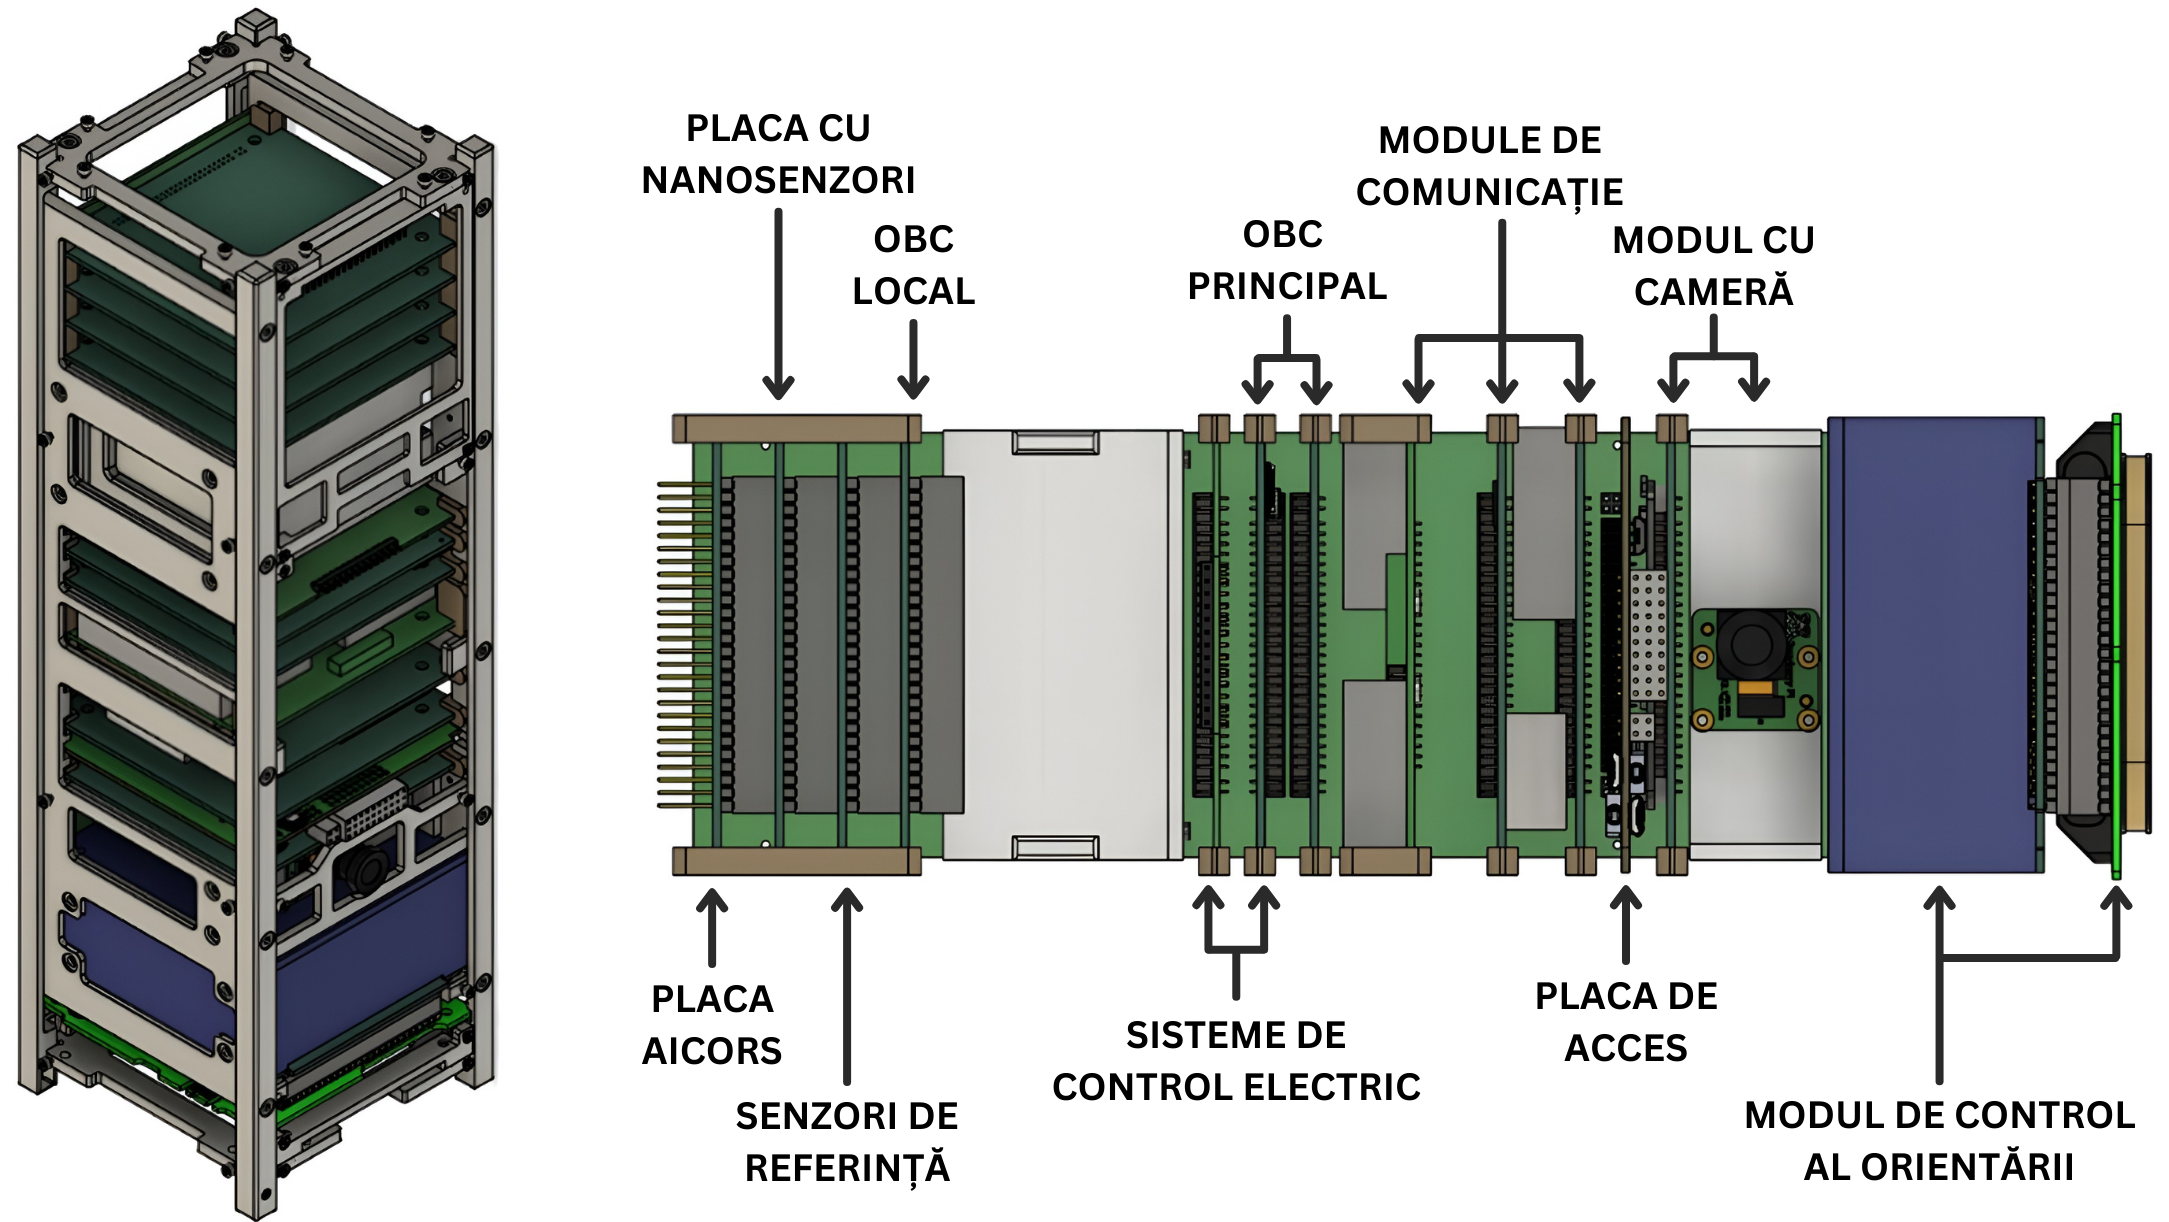
\includegraphics[width=\columnwidth]{./Images/conclusion_birds_sat.png}
    \caption{Structura nanosatelitului de tip 3U BIRDS-RPM. Adaptată din \cite{birds_presentation}}%
    \label{fig:conclusion_birds_sat}
\end{figure}
\newpage

În al doilea rând, colaborarea cu Universitatea Tehnică a Moldovei s-a dovedit a fi eficientă și benefică. Aceasta a contribuit la accelerarea procesului de dezvoltare și cercetare și a oferit acces la expertiză în domeniul fizicii radiației, al dezvoltării sistemelor electronice pentru aplicații spațiale și al dezvoltării nanosateliților. De asemenea, studenții implicați în proiect, printre care mă număr și eu, au avut oportunitatea de a participa activ într-o echipă de cercetare, având oportunitatea de a contribui la îmbunătățirea sistemului și de a dobândi experiență practică în proiectarea, testarea și validarea sistemelor \gls{fpga} pentru aplicații spațiale.

\section{Limitări și direcții viitoare}
Deși proiectul a fost în mare parte un succes, există în continuare limitări și direcții clare de îmbunătățire care pot crește performanța și robustețea plăcii \gls{aicors}. O primă direcție importantă este extinderea mecanismelor de redundanță și protecție, atât la nivel logic, cât și la nivel electric. În plus, o direcție naturală a sistemului ar fi implementarea unui model de inteligență artificială direct pe dispozitivul \gls{fpga}, capabil să clasifice și să grupeze evenimentele de tip \gls{seu} în informații mai relevante. Un astfel de model ar putea estima nivelul curent de radiație sau chiar prezice evoluția nivelului de radiație pe baza tendințelor recente.

O limitare majoră a proiectului a fost lipsa accesului la o sursă de radiație controlată pentru testarea experimentală. Aceste teste ar putea oferi informații valoroase privind robustețea sistemului și susceptibilitatea reală a configurării \gls{fpga}-ului și a \gls{pcb}-ului la radiație, permițând optimizarea proiectului pentru mediul spațial. Dacă în viitor va exista acces la un centru de iradiere, testarea ar fi relativ simplă de realizat, deoarece placa nu necesită module exterioare adiționale, ci alimentare și un cablu de comunicație \gls{spi}. În cazul utilizării primei versiuni a \gls{pcb}-ului, datele achiziționate pot fi stocate local pe un card SD, fiind necesară doar alimentarea plăcii. O altă variantă pentru testare este realizarea unui experiment cu balon meteorologic. Acesta ar implica, pe lângă balon, integrarea plăcii într-un sistem ce include module de localizare, baterii și eventual alți senzori. Un astfel de experiment ar oferi o aproximare mai realistă a mediului spațial și ar oferi informații adiționale privind comportamentul plăcii \gls{aicors} în condiții mai dificile, cu vibrații, presiune scăzută și niveluri crescute de zgomot electromagnetic.

O altă direcție de dezvoltare este utilizarea plăcii \gls{aicors} pentru implementarea altor sisteme rezistente la radiație. De exemplu, se poate integra un procesor MicroBlaze sau un procesor personalizat, protejat prin tehnici împotriva radiației, precum \gls{tmr}. Acesta poate fi ulterior folosit fie ca alternativă de procesor principal într-un sistem tolerant la radiație în cadrul altor proiecte, fie în paralel cu sistemul actual, pentru controlul plăcii \gls{aicors} sau pentru implementarea unui model AI pentru procesarea inteligentă a datelor colectate.

Astfel, prin aceste extinderi, placa \gls{aicors} poate evolua de la un simplu senzor de radiație la un sistem activ de monitorizare și suport, utilizabil atât pentru nanosateliți, cât și pentru aplicații terestre de cercetare.

\section{Publicații rezultate din acest proiect}
Activitatea desfășurată în cadrul acestui proiect a condus la publicarea mai multor lucrări științifice, care abordează diferite etape, rezultate și aspecte relevante din dezvoltarea sistemului. Lista acestora este prezentată mai jos:

\begin{itemize}
    \item Este prezentată problema abordată de proiectul \gls{aicors}, împreună cu o versiune preliminară a algoritmului de detecție a evenimentelor \gls{seu}: \fullcite{isetc}
    \item Sunt descrise arhitectura generală a proiectului BIRDS, structura senzorului de radiație bazat pe \gls{fpga}, precum și o analiză comparativă a principalelor opțiuni pentru \gls{fpga}: \fullcite{jes}
    \item Se prezintă structura primei versiuni a \gls{pcb}-ului, modulele principale și etapele de dezvoltare ale proiectului: \fullcite{icemes}
    \item Este realizat un studiu al consumului de energie al dispozitivului \gls{fpga} și al primei versiuni a \gls{pcb}-ului \gls{aicors}, pentru diferite implementări ale proiectului Verilog: \fullcite{icecs}
\end{itemize}

% ------- BIBLIOGRAPHY IS AUTOMATED - NO NEED TO MODIFY
\printbibliography

\chapter*{Rezumat}
\addcontentsline{toc}{chapter}{Rezumat}

În mediul spațial terestru există un nivel ridicat de radiație, provenit din surse precum \acrfull{gcr}, evenimente solare și particule captate în magnetosfera Pământului. Interacțiunea acestor particule cu circuitele electronice poate produce efecte permanente sau efecte temporare de tip \acrfull{see}, dintre care cele mai frecvente sunt \acrfull{seu} și \acrfull{set}. Aceste efecte reprezintă o problemă majoră pentru sistemele critice și de înaltă performanță utilizate în misiuni spațiale, fiind necesare metode dedicate pentru detectarea nivelului de radiație și pentru creșterea fiabilității acestora. Această lucrare prezintă proiectarea, implementarea și validarea unei plăci senzor pentru radiație cosmică, bazată pe un dispozitiv de tip \acrfull{fpga}. Proiectul face parte din PN-IV-P8-8.3- ROMD-2023-0068 intitulat „Artificial Intelligence-enabled Hardware Cosmic Radiation Sensor for Space Applications (AICoRS)”, desfășurat în parteneriat între Universitatea Transilvania din Brașov și Universitatea Tehnică a Moldovei. Lucrarea descrie întregul proces de dezvoltare al sistemului, incluzând selecția \gls{fpga}-ului ideal, dezvoltarea codului \acrfull{hdl} pentru detecția \gls{seu}-urilor și pentru comunicație, proiectarea unui \acrfull{pcb} suport pentru integrarea într-un nanosatelit, precum și testarea și validarea tuturor componentelor. De asemenea, este prezentată o parte teoretică privind mediul de radiație spațială, împreună cu metodele de conversie a parametrilor fizici ai acestuia în rate de modificare a biților din memoriile dispozitivului. Placa dezvoltată a trecut cu succes prin etapele de proiectare și validare și va fi integrată, alături de alte două plăci detectoare de radiații și un \acrfull{obc} local, ca payload moldovenesc în nanosatelitul BIRDS-RPM de tip 3U, în cadrul programului BIRDS. Satelitul urmează să fie lansat în \acrfull{leo} în cadrul unei misiuni de reaprovizionare a Stației Spațiale Internaționale (\gls{iss}) de către \acrfull{jaxa}.

\chapter*{Abstract}
\addcontentsline{toc}{chapter}{Abstract}

In the terrestrial space environment, there is a high level of radiation originating from sources such as \acrfull{gcr}, solar events, and particles captured in the Earth's magnetosphere. The interaction of these particles with electronic circuits can cause permanent or temporary effects known as Single Event Effects (\gls{see}), mainly Single Event Upsets (\gls{seu}) and Single Event Transients (\gls{set}). These effects are a major problem for critical and high-performance systems used in space missions, requiring dedicated methods for detecting radiation levels and increasing system reliability. This paper describes the design, implementation, and validation of a cosmic radiation sensor board based on a \acrfull{fpga} device. The project is part of PN-IV-P8-8.3-ROMD-2023-0068 entitled "Artificial Intelligence-enabled Hardware Cosmic Radiation Sensor for Space Applications (AICoRS)", carried out in partnership between Transilvania University of Brașov and the Technical University of Moldova. The paper describes the entire system development process, including ideal FPGA selection, the development of \acrfull{hdl} code for \gls{seu} detection and communication, the design of a \acrfull{pcb} for integration into a nanosatellite, as well as the testing and validation of all components. It also presents a theoretical part on the space radiation environment, along with methods for converting its physical parameters into bit change rates in the device's memories. The developed board has successfully passed the design and validation stages and will be integrated, along with two other radiation detector boards and a local \acrfull{obc}, as a Moldovan payload in the 3U BIRDS-RPM nanosatellite, as part of the BIRDS program. The satellite is scheduled to be launched in \acrfull{leo} as part of a resupply mission to the International Space Station (\gls{iss}) by the Japan Aerospace Exploration Agency (\gls{jaxa}).

\end{document}
